\documentclass[twoside]{book}

% Packages required by doxygen
\usepackage{fixltx2e}
\usepackage{calc}
\usepackage{doxygen}
\usepackage[export]{adjustbox} % also loads graphicx
\usepackage{graphicx}
\usepackage[utf8]{inputenc}
\usepackage{makeidx}
\usepackage{multicol}
\usepackage{multirow}
\PassOptionsToPackage{warn}{textcomp}
\usepackage{textcomp}
\usepackage[nointegrals]{wasysym}
\usepackage[table]{xcolor}

% Font selection
\usepackage[T1]{fontenc}
\usepackage[scaled=.90]{helvet}
\usepackage{courier}
\usepackage{amssymb}
\usepackage{sectsty}
\renewcommand{\familydefault}{\sfdefault}
\allsectionsfont{%
  \fontseries{bc}\selectfont%
  \color{darkgray}%
}
\renewcommand{\DoxyLabelFont}{%
  \fontseries{bc}\selectfont%
  \color{darkgray}%
}
\newcommand{\+}{\discretionary{\mbox{\scriptsize$\hookleftarrow$}}{}{}}

% Page & text layout
\usepackage{geometry}
\geometry{%
  a4paper,%
  top=2.5cm,%
  bottom=2.5cm,%
  left=2.5cm,%
  right=2.5cm%
}
\tolerance=750
\hfuzz=15pt
\hbadness=750
\setlength{\emergencystretch}{15pt}
\setlength{\parindent}{0cm}
\setlength{\parskip}{3ex plus 2ex minus 2ex}
\makeatletter
\renewcommand{\paragraph}{%
  \@startsection{paragraph}{4}{0ex}{-1.0ex}{1.0ex}{%
    \normalfont\normalsize\bfseries\SS@parafont%
  }%
}
\renewcommand{\subparagraph}{%
  \@startsection{subparagraph}{5}{0ex}{-1.0ex}{1.0ex}{%
    \normalfont\normalsize\bfseries\SS@subparafont%
  }%
}
\makeatother

% Headers & footers
\usepackage{fancyhdr}
\pagestyle{fancyplain}
\fancyhead[LE]{\fancyplain{}{\bfseries\thepage}}
\fancyhead[CE]{\fancyplain{}{}}
\fancyhead[RE]{\fancyplain{}{\bfseries\leftmark}}
\fancyhead[LO]{\fancyplain{}{\bfseries\rightmark}}
\fancyhead[CO]{\fancyplain{}{}}
\fancyhead[RO]{\fancyplain{}{\bfseries\thepage}}
\fancyfoot[LE]{\fancyplain{}{}}
\fancyfoot[CE]{\fancyplain{}{}}
\fancyfoot[RE]{\fancyplain{}{\bfseries\scriptsize Generated by Doxygen }}
\fancyfoot[LO]{\fancyplain{}{\bfseries\scriptsize Generated by Doxygen }}
\fancyfoot[CO]{\fancyplain{}{}}
\fancyfoot[RO]{\fancyplain{}{}}
\renewcommand{\footrulewidth}{0.4pt}
\renewcommand{\chaptermark}[1]{%
  \markboth{#1}{}%
}
\renewcommand{\sectionmark}[1]{%
  \markright{\thesection\ #1}%
}

% Indices & bibliography
\usepackage{natbib}
\usepackage[titles]{tocloft}
\setcounter{tocdepth}{3}
\setcounter{secnumdepth}{5}
\makeindex

% Hyperlinks (required, but should be loaded last)
\usepackage{ifpdf}
\ifpdf
  \usepackage[pdftex,pagebackref=true]{hyperref}
\else
  \usepackage[ps2pdf,pagebackref=true]{hyperref}
\fi
\hypersetup{%
  colorlinks=true,%
  linkcolor=blue,%
  citecolor=blue,%
  unicode%
}

% Custom commands
\newcommand{\clearemptydoublepage}{%
  \newpage{\pagestyle{empty}\cleardoublepage}%
}

\usepackage{caption}
\captionsetup{labelsep=space,justification=centering,font={bf},singlelinecheck=off,skip=4pt,position=top}

%===== C O N T E N T S =====

\begin{document}

% Titlepage & ToC
\hypersetup{pageanchor=false,
             bookmarksnumbered=true,
             pdfencoding=unicode
            }
\pagenumbering{alph}
\begin{titlepage}
\vspace*{7cm}
\begin{center}%
{\Large Ego\+Video\+Stabilizer \\[1ex]\large 1.\+0.\+0 }\\
\vspace*{1cm}
{\large Generated by Doxygen 1.8.12}\\
\end{center}
\end{titlepage}
\clearemptydoublepage
\pagenumbering{roman}
\tableofcontents
\clearemptydoublepage
\pagenumbering{arabic}
\hypersetup{pageanchor=true}

%--- Begin generated contents ---
\chapter{General Information}
\label{index}\hypertarget{index}{}\hypertarget{index_project_sec}{}\section{Project}\label{index_project_sec}
This code is based on the paper \href{http://www.verlab.dcc.ufmg.br/wp-content/uploads/2016/10/Final_Draft_ECCVW_2016_Towards_Semantic_Fast_Forward_and_Stabilied_Egocentric_Videos.pdf}{\tt Towards Semantic Fast-\/\+Forward and Stabilized Egocentric Video} on the {\bfseries First International Workshop on Egocentric Perception, Interaction and Computing} at {\bfseries European Conference on Computer Vision} (E\+P\+IC@E\+C\+CV 2016). The goal of the program is to stabilize a fast-\/forward version of a video, using the dropped frames to reconstruct distorted images during the processing.

For more information, acess the link\+: \href{http://www.verlab.dcc.ufmg.br/fast-forward-video-based-on-semantic-extraction/}{\tt http\+://www.\+verlab.\+dcc.\+ufmg.\+br/fast-\/forward-\/video-\/based-\/on-\/semantic-\/extraction/}. ~\newline
 \hypertarget{index_contact_sec}{}\section{Contact}\label{index_contact_sec}
\hypertarget{index_authors_sec}{}\subsection{Authors\+:}\label{index_authors_sec}
\begin{DoxyItemize}
\item Michel Melo da Silva -\/ PhD student -\/ U\+F\+MG -\/ \href{mailto:michelms@dcc.ufmg.com}{\tt michelms@dcc.\+ufmg.\+com} \item Washington Luis de Souza Ramos -\/ M\+Sc student -\/ U\+F\+MG -\/ \href{mailto:washington.ramos@outlook.com}{\tt washington.\+ramos@outlook.\+com} \item João Pedro Klock Ferreira -\/ Undergraduate Student -\/ U\+F\+MG -\/ \href{mailto:jpklock@dcc.ufmg.br}{\tt jpklock@dcc.\+ufmg.\+br} \item Mario Fernando Montenegro Campos -\/ Advisor -\/ U\+F\+MG -\/ \href{mailto:mario@dcc.ufmg.br}{\tt mario@dcc.\+ufmg.\+br} \item Erickson Rangel do Nascimento -\/ Advisor -\/ U\+F\+MG -\/ \href{mailto:erickson@dcc.ufmg.br}{\tt erickson@dcc.\+ufmg.\+br}\end{DoxyItemize}
\hypertarget{index_institution_sec}{}\subsection{Institution}\label{index_institution_sec}
Federal University of Minas Gerais (U\+F\+MG) ~\newline
Computer Science Department ~\newline
Belo Horizonte -\/ Minas Gerais -\/\+Brazil\hypertarget{index_laboratory_subsec}{}\subsection{Laboratory}\label{index_laboratory_subsec}
{\bfseries Ve\+R\+Lab\+:} Vison and Robotic Laboratory ~\newline
\href{http://www.verlab.dcc.ufmg.br}{\tt http\+://www.\+verlab.\+dcc.\+ufmg.\+br}\hypertarget{index_program_sec}{}\section{Program}\label{index_program_sec}
\hypertarget{index_dependencies_sec}{}\subsection{Dependencies}\label{index_dependencies_sec}
\begin{DoxyItemize}
\item Open\+CV 2.\+4.\+X {\itshape (Tested with 2.\+4.\+9 and 2.\+4.\+13)} \item Armadillo 6.\+X {\itshape (Tested with 6.\+600.\+5 -- Catabolic Amalgamator)} \item Boost 1.\+X {\itshape (Tested with 1.\+54.\+0)}\end{DoxyItemize}
\hypertarget{index_compiling_sec}{}\subsection{Compiling}\label{index_compiling_sec}
The program can be compiled using either {\ttfamily cmake} or {\ttfamily qmake} tools. Into the project directory, run the following commands\+:

{\ttfamily  {\bfseries user@computer\+:$<$project\+\_\+path$>$\+:} mkdir build ~\newline
{\bfseries user@computer\+:$<$project\+\_\+path$>$\+:} cd build ~\newline
{\bfseries user@computer\+:$<$project\+\_\+path$>$\+:} cmake .. ~\newline
{\bfseries user@computer\+:$<$project\+\_\+path$>$\+:} make ~\newline
{\bfseries user@computer\+:$<$project\+\_\+path$>$\+:} ./\+Video\+Stabilization $<$ Settings\+\_\+file $>$ \mbox{[}-\/h\mbox{]} \mbox{[}Range\+\_\+min\mbox{]} \mbox{[}Range\+\_\+max\mbox{]}~\newline
}\hypertarget{index_execution_sec}{}\subsection{Exemples of usage}\label{index_execution_sec}
{\ttfamily  $<$ Program\+\_\+name $>$ $<$ Settings\+\_\+file $>$ \mbox{[}-\/h\mbox{]} \mbox{[}Range\+\_\+min = 0 \mbox{]} \mbox{[}Range\+\_\+max = num\+\_\+frames \mbox{]} } ~\newline
~\newline
Example 1\+: Run Video\+Stabilization using Help option. ~\newline
{\ttfamily  -\/$>$ Video\+Stabilization -\/h } ~\newline
~\newline
Example 2\+: Run Video\+Stabilization in the Experiment\+\_\+1 processing the whole video. ~\newline
{\ttfamily  -\/$>$ Video\+Stabilization Experiment\+\_\+1.\+xml } ~\newline
~\newline
Example 3\+: Run Video\+Stabilization in the Experiment\+\_\+1 processing from the 150 frame until the last one. ~\newline
{\ttfamily  -\/$>$ Video\+Stabilization Experiment\+\_\+1.\+xml {\ttfamily 150} } ~\newline
~\newline
Example 4\+: Run Video\+Stabilization in the Experiment\+\_\+1 processing from the 150 frame until the frame 490. ~\newline
{\ttfamily  -\/$>$ Video\+Stabilization Experiment\+\_\+1.\+xml 150 490 } ~\newline
~\newline
 \hypertarget{index_citation_sec}{}\section{Citation}\label{index_citation_sec}
If you are using it to academic purpose, please cite\+: ~\newline
 M. M. Silva, W. L. S. Ramos, J. P. K. Ferreira, M. F. M. Campos, E. R. Nascimento, {\bfseries Towards semantic fast-\/forward and stabilized egocentric videos}, in\+: European Conference on Computer Vision Workshops, Springer International Publishing, Amsterdam, NL, 2016, pp. 557–571. doi\+:10.\+1007/978-\/3-\/319-\/46604-\/0\+\_\+40.\hypertarget{index_bibtex_subsec}{}\subsection{Bibtex entry}\label{index_bibtex_subsec}
{\ttfamily  @In\+Book\{Silva2016, ~\newline
 Title = \{Towards Semantic Fast-\/\+Forward and Stabilized Egocentric Videos\}, ~\newline
 Author = \{Silva, Michel Melo and Ramos, Washington Luis Souza and Ferreira, ~\newline
 Joao Pedro Klock and Campos, Mario Fernando Montenegro and Nascimento, Erickson Rangel\}, ~\newline
 Editor = \{Hua, Gang and J\{\textbackslash{}\textquotesingle{}e\}gou, Herv\{\textbackslash{}\textquotesingle{}e\}\}, ~\newline
 Pages = \{557--571\}, ~\newline
 Publisher = \{Springer International Publishing\}, ~\newline
 Year = \{2016\}, ~\newline
 Address = \{Cham\}, ~\newline
 Booktitle = \{Computer Vision -- E\+C\+CV 2016 Workshops\+: Amsterdam, The Netherlands, ~\newline
 October 8-\/10 and 15-\/16, 2016, Proceedings, Part I\}, ~\newline
 Doi = \{10.\+1007/978-\/3-\/319-\/46604-\/0\+\_\+40\}, ~\newline
 I\+S\+BN = \{978-\/3-\/319-\/46604-\/0\}, ~\newline
 Url = \{\href{http://dx.doi.org/10.1007/978-3-319-46604-0_40}{\tt http\+://dx.\+doi.\+org/10.\+1007/978-\/3-\/319-\/46604-\/0\+\_\+40}\} ~\newline
\} } 
\chapter{doc\+\_\+mainpage}
\label{md_doc_doc_mainpage}
\hypertarget{md_doc_doc_mainpage}{}
\input{md_doc_doc_mainpage}
\chapter{Project}
\label{md_README}
\hypertarget{md_README}{}
This code is based on the paper \href{http://www.verlab.dcc.ufmg.br/wp-content/uploads/2016/10/Final_Draft_ECCVW_2016_Towards_Semantic_Fast_Forward_and_Stabilied_Egocentric_Videos.pdf}{\tt Towards Semantic Fast-\/\+Forward and Stabilized Egocentric Video} on the {\bfseries First International Workshop on Egocentric Perception, Interaction and Computing} at {\bfseries European Conference on Computer Vision} (E\+P\+IC@E\+C\+CV 2016). The goal of the program is to stabilize a fast-\/forward version of a video, using the dropped frames to reconstruct distorted images during the processing.

For more information, acess the link\+: \href{http://www.verlab.dcc.ufmg.br/fast-forward-video-based-on-semantic-extraction}{\tt http\+://www.\+verlab.\+dcc.\+ufmg.\+br/fast-\/forward-\/video-\/based-\/on-\/semantic-\/extraction}.

\subsection*{Contact}

\subsubsection*{Authors}


\begin{DoxyItemize}
\item Michel Melo da Silva -\/ PhD student -\/ U\+F\+MG -\/ \href{mailto:michelms@dcc.ufmg.com}{\tt michelms@dcc.\+ufmg.\+com}
\item Washington Luis de Souza Ramos -\/ M\+Sc student -\/ U\+F\+MG -\/ \href{mailto:washington.ramos@outlook.com}{\tt washington.\+ramos@outlook.\+com}
\item Jo�o Pedro Klock Ferreira -\/ Undergraduate Student -\/ U\+F\+MG -\/ \href{mailto:jpklock@dcc.ufmg.br}{\tt jpklock@dcc.\+ufmg.\+br}
\item Mario Fernando Montenegro Campos -\/ Advisor -\/ U\+F\+MG -\/ \href{mailto:mario@dcc.ufmg.br}{\tt mario@dcc.\+ufmg.\+br}
\item Erickson Rangel do Nascimento -\/ Advisor -\/ U\+F\+MG -\/ \href{mailto:erickson@dcc.ufmg.br}{\tt erickson@dcc.\+ufmg.\+br}
\end{DoxyItemize}

\subsubsection*{Institution}

Federal University of Minas Gerais (U\+F\+MG) Computer Science Department Belo Horizonte -\/ Minas Gerais -\/\+Brazil

\subsubsection*{Laboratory}

{\bfseries Ve\+R\+Lab\+:} Vison and Robotic Laboratory \href{http://www.verlab.dcc.ufmg.br}{\tt http\+://www.\+verlab.\+dcc.\+ufmg.\+br}

\subsection*{Program}

\subsubsection*{Dependencies}


\begin{DoxyItemize}
\item Open\+CV 2.\+4 \+\_\+(Tested with 2.\+4.\+9 and 2.\+4.\+13)\+\_\+
\item Armadillo 6 \+\_\+(Tested with 6.\+600.\+5 -- Catabolic Amalgamator)\+\_\+
\item Boost 1 \+\_\+(Tested with 1.\+54.\+0)\+\_\+
\item Doxygen 1 \+\_\+(for documentation -\/ Tested with 1.\+8.\+12)\+\_\+
\end{DoxyItemize}

\subsubsection*{Compiling}

The program can be compiled using either {\ttfamily cmake} or {\ttfamily qmake} tools.

Into the project directory, run the following commands\+: \begin{DoxyVerb}        user@computer:<project_path>: mkdir build 
        user@computer:<project_path>: cd build
        user@computer:<project_path/build>: cmake ..
        user@computer:<project_path/build>: make
        user@computer:<project_path/build>: ./VideoStabilization < Settings_file > [-h] [Range_min] [Range_max]
\end{DoxyVerb}


\subsubsection*{Exemples of usage}

\begin{DoxyVerb}        user@computer:<project_path/build>: < Program_name > < Settings_file > [-h] [Range_min = 0 ] [Range_max = num_frames ]
\end{DoxyVerb}


Example 1\+: Run Video\+Stabilization using Help option. \begin{DoxyVerb}        user@computer:<project_path/build>: ./VideoStabilization -h 
\end{DoxyVerb}


Example 2\+: Run Video\+Stabilization in the Experiment\+\_\+1 processing the whole video. \begin{DoxyVerb}        user@computer:<project_path/build>: ./VideoStabilization Experiment_1.xml
\end{DoxyVerb}


Example 3\+: Run Video\+Stabilization in the Experiment\+\_\+1 processing from the 150 frame until the last one. \begin{DoxyVerb}        user@computer:<project_path/build>: ./VideoStabilization Experiment_1.xml 150 
\end{DoxyVerb}


Example 4\+: Run Video\+Stabilization in the Experiment\+\_\+1 processing from the 150 frame until the frame 490. \begin{DoxyVerb}        user@computer:<project_path/build>: ./VideoStabilization Experiment_1.xml 150 490
\end{DoxyVerb}


\subsubsection*{Documentation}

To generate the documentation of the project, run the following command into the project folder\+: \begin{DoxyVerb}        user@computer:<project_path>: doxygen doc/doc_conf
\end{DoxyVerb}


The documentation will be generated in the {\ttfamily $<$project\+\_\+path$>$/doc} folder.

\subsection*{Citation}

If you are using it to academic purpose, please cite\+:

M. M. Silva, W. L. S. Ramos, J. P. K. Ferreira, M. F. M. Campos, E. R. Nascimento, {\bfseries Towards semantic fast-\/forward and stabilized egocentric videos}, in\+: European Conference on Computer Vision Workshops, Springer International Publishing, Amsterdam, NL, 2016, pp. 557�571. doi\+:10.\+1007/978-\/3-\/319-\/46604-\/0\+\_\+40.

\subsubsection*{Bibtex entry}

\begin{quote}
\{Silva2016, Title = \{Towards Semantic Fast-\/\+Forward and Stabilized Egocentric Videos\}, Author = \{Silva, Michel Melo and Ramos, Washington Luis Souza and Ferreira,Joao Pedro Klock and Campos, Mario Fernando Montenegro and Nascimento, Erickson Rangel\}, Editor = \{Hua, Gang and J\{\textbackslash{}\textquotesingle{}e\}gou, Herv\{\textbackslash{}\textquotesingle{}e\}\}, Pages = \{557--571\}, Publisher = \{Springer International Publishing\}, Year = \{2016\}, Address = \{Cham\}, Booktitle = \{Computer Vision -- E\+C\+CV 2016 Workshops\+: Amsterdam, The Netherlands, October 8-\/10 and 15-\/16, 2016, Proceedings, Part I\}, Doi = \{10.\+1007/978-\/3-\/319-\/46604-\/0\+\_\+40\}, I\+S\+BN = \{978-\/3-\/319-\/46604-\/0\}, Url = \{\href{http://dx.doi.org/10.1007/978-3-319-46604-0_40}{\tt http\+://dx.\+doi.\+org/10.\+1007/978-\/3-\/319-\/46604-\/0\+\_\+40}\} \} \end{quote}


\subparagraph*{Enjoy it.}
\chapter{Class Index}
\section{Class List}
Here are the classes, structs, unions and interfaces with brief descriptions\+:\begin{DoxyCompactList}
\item\contentsline{section}{\hyperlink{structEXPERIMENT}{E\+X\+P\+E\+R\+I\+M\+E\+NT} }{\pageref{structEXPERIMENT}}{}
\item\contentsline{section}{\hyperlink{classMessageHandler}{Message\+Handler} }{\pageref{classMessageHandler}}{}
\end{DoxyCompactList}

\chapter{File Index}
\section{File List}
Here is a list of all files with brief descriptions\+:\begin{DoxyCompactList}
\item\contentsline{section}{definitions/\hyperlink{define_8h}{define.\+h} \\*Macros used in the code relate with debug/view flags and usual values }{\pageref{define_8h}}{}
\item\contentsline{section}{definitions/\hyperlink{experiment__struct_8h}{experiment\+\_\+struct.\+h} \\*Fields declaration of the experiment settings }{\pageref{experiment__struct_8h}}{}
\item\contentsline{section}{definitions/\hyperlink{experiments_8h}{experiments.\+h} \\*Definitions of experiment settings }{\pageref{experiments_8h}}{}
\item\contentsline{section}{executables/\hyperlink{execute__commands_8h}{execute\+\_\+commands.\+h} \\*Macro with specific codes }{\pageref{execute__commands_8h}}{}
\item\contentsline{section}{headers/\hyperlink{error__messages_8h}{error\+\_\+messages.\+h} }{\pageref{error__messages_8h}}{}
\item\contentsline{section}{headers/\hyperlink{file__operations_8h}{file\+\_\+operations.\+h} \\*Header functions for the \hyperlink{file__operations_8cpp}{file\+\_\+operations.\+cpp} }{\pageref{file__operations_8h}}{}
\item\contentsline{section}{headers/\hyperlink{homography_8h}{homography.\+h} \\*Header functions for the \hyperlink{homography_8cpp}{homography.\+cpp} }{\pageref{homography_8h}}{}
\item\contentsline{section}{headers/\hyperlink{image__reconstruction_8h}{image\+\_\+reconstruction.\+h} \\*Header functions for the \hyperlink{image__reconstruction_8cpp}{image\+\_\+reconstruction.\+cpp} }{\pageref{image__reconstruction_8h}}{}
\item\contentsline{section}{headers/\hyperlink{line__and__point__operations_8h}{line\+\_\+and\+\_\+point\+\_\+operations.\+h} \\*Header functions for the \hyperlink{line__and__point__operations_8cpp}{line\+\_\+and\+\_\+point\+\_\+operations.\+cpp} }{\pageref{line__and__point__operations_8h}}{}
\item\contentsline{section}{headers/\hyperlink{master__frames_8h}{master\+\_\+frames.\+h} \\*Header functions for the \hyperlink{master__frames_8cpp}{master\+\_\+frames.\+cpp} }{\pageref{master__frames_8h}}{}
\item\contentsline{section}{headers/\hyperlink{message__handler_8h}{message\+\_\+handler.\+h} }{\pageref{message__handler_8h}}{}
\item\contentsline{section}{headers/\hyperlink{sequence__processing_8h}{sequence\+\_\+processing.\+h} \\*Header functions for the \hyperlink{sequence__processing_8cpp}{sequence\+\_\+processing.\+cpp} }{\pageref{sequence__processing_8h}}{}
\item\contentsline{section}{src/\hyperlink{file__operations_8cpp}{file\+\_\+operations.\+cpp} \\*Functions to manipulate files }{\pageref{file__operations_8cpp}}{}
\item\contentsline{section}{src/\hyperlink{homography_8cpp}{homography.\+cpp} \\*Functions related with homography transformation }{\pageref{homography_8cpp}}{}
\item\contentsline{section}{src/\hyperlink{image__reconstruction_8cpp}{image\+\_\+reconstruction.\+cpp} \\*Functions related with reconstruction of the image after application of the homography matrix to fill the whole frame boundaries }{\pageref{image__reconstruction_8cpp}}{}
\item\contentsline{section}{src/\hyperlink{line__and__point__operations_8cpp}{line\+\_\+and\+\_\+point\+\_\+operations.\+cpp} \\*Functions to handle line and point functions }{\pageref{line__and__point__operations_8cpp}}{}
\item\contentsline{section}{src/\hyperlink{line__and__points__operations_8cpp}{line\+\_\+and\+\_\+points\+\_\+operations.\+cpp} }{\pageref{line__and__points__operations_8cpp}}{}
\item\contentsline{section}{src/\hyperlink{main_8cpp}{main.\+cpp} \\*Main file that contains the \hyperlink{main_8cpp}{main.\+cpp} }{\pageref{main_8cpp}}{}
\item\contentsline{section}{src/\hyperlink{master__frames_8cpp}{master\+\_\+frames.\+cpp} \\*Functions to get the master frames from file or calculating it }{\pageref{master__frames_8cpp}}{}
\item\contentsline{section}{src/\hyperlink{message__handler_8cpp}{message\+\_\+handler.\+cpp} }{\pageref{message__handler_8cpp}}{}
\item\contentsline{section}{src/\hyperlink{sequence__processing_8cpp}{sequence\+\_\+processing.\+cpp} \\*Functions related with sequence processing, such as find intermediate homography, get transition weight, select new frame }{\pageref{sequence__processing_8cpp}}{}
\end{DoxyCompactList}

\chapter{Class Documentation}
\hypertarget{structEXPERIMENT}{}\section{E\+X\+P\+E\+R\+I\+M\+E\+NT Struct Reference}
\label{structEXPERIMENT}\index{E\+X\+P\+E\+R\+I\+M\+E\+NT@{E\+X\+P\+E\+R\+I\+M\+E\+NT}}


{\ttfamily \#include $<$experiment\+\_\+struct.\+h$>$}

\subsection*{Public Attributes}
\begin{DoxyCompactItemize}
\item 
std\+::string \hyperlink{structEXPERIMENT_af59b6805fe0851b89d1300849db794e4}{id}
\item 
std\+::string \hyperlink{structEXPERIMENT_a7095f959a6d88f3a5997bcd0f4579609}{video\+\_\+filename}
\item 
std\+::string \hyperlink{structEXPERIMENT_a05ae2a5fbc8660bdb535937d4a446698}{output\+\_\+path}
\begin{DoxyCompactList}\small\item\em Complete path and filename of the video with extension. \end{DoxyCompactList}\item 
std\+::string \hyperlink{structEXPERIMENT_a3ce2700a31e4c1b808caceab4626ff06}{original\+\_\+video\+\_\+filename}
\begin{DoxyCompactList}\small\item\em Complete path to the folder where the results will be saved. \end{DoxyCompactList}\item 
std\+::string \hyperlink{structEXPERIMENT_a3412818ed24d2c956b01e1d6561d7b50}{read\+\_\+master\+\_\+frames\+\_\+filename}
\begin{DoxyCompactList}\small\item\em Complete path and filename of the original video. \end{DoxyCompactList}\item 
std\+::string \hyperlink{structEXPERIMENT_af3623d64105d92bec8a761c5318ec534}{save\+\_\+master\+\_\+frames\+\_\+filename}
\begin{DoxyCompactList}\small\item\em Complete path and filename of the txt file with the selected master frames. \end{DoxyCompactList}\item 
std\+::string \hyperlink{structEXPERIMENT_a867146c43457a82a6b2346d8621d70b6}{save\+\_\+video\+\_\+filename}
\begin{DoxyCompactList}\small\item\em Complete path and filename to save the txt file with the selected master frames. \end{DoxyCompactList}\item 
std\+::string \hyperlink{structEXPERIMENT_aef88dd45b0ad1db5f6b68b0801f6f630}{selected\+\_\+frames\+\_\+filename}
\begin{DoxyCompactList}\small\item\em Complete path and filename of the save the stabilized video. \end{DoxyCompactList}\item 
std\+::string \hyperlink{structEXPERIMENT_ab71731194cb1680b25dd9ed253e455aa}{semantic\+\_\+costs\+\_\+filename}
\begin{DoxyCompactList}\small\item\em Complete path and filename of the csv file with the selected master frames that was selected to create the reduced video. \end{DoxyCompactList}\item 
std\+::string \hyperlink{structEXPERIMENT_a74bd001a4012183b8dacec4e79315a13}{instability\+\_\+costs\+\_\+filename}
\begin{DoxyCompactList}\small\item\em Complete path and filename of the csv file with the semantic costs of the frame transitions. \end{DoxyCompactList}\item 
std\+::string \hyperlink{structEXPERIMENT_a8b5ca464e785c2b80c16c9e022b7c31a}{optical\+\_\+flow\+\_\+filename}
\begin{DoxyCompactList}\small\item\em Complete path and filename of the csv file with the jitter costs of the transitions. \end{DoxyCompactList}\item 
std\+::string \hyperlink{structEXPERIMENT_ac3568164588c0366d26fc9cd69b98fe3}{log\+\_\+file\+\_\+name}
\begin{DoxyCompactList}\small\item\em Complete path and filename of the csv file with the optical flow calculated by the Flow\+Net. \end{DoxyCompactList}\item 
int \hyperlink{structEXPERIMENT_a004195c9cb30dde7a5cac231381503da}{segment\+\_\+size}
\begin{DoxyCompactList}\small\item\em Complete path and filename to save the txt file log execution. \end{DoxyCompactList}\item 
bool \hyperlink{structEXPERIMENT_a665b9063cc9475513a16db5b1c7f10a1}{save\+\_\+master\+\_\+frames\+\_\+in\+\_\+disk}
\begin{DoxyCompactList}\small\item\em Size of the segments where the master frames will be calculated. \end{DoxyCompactList}\item 
bool \hyperlink{structEXPERIMENT_aa392d503b8f79c0d0ee6168226245dd1}{save\+\_\+video\+\_\+in\+\_\+disk}
\begin{DoxyCompactList}\small\item\em After calculte the master frames, do you want to save it in a file? After you can load it directly withou calculate again. \end{DoxyCompactList}\item 
bool \hyperlink{structEXPERIMENT_a74a95ad0fdb8e786e1555bcb4053af2e}{running\+\_\+parallel}
\begin{DoxyCompactList}\small\item\em Save stabilized video in Disk. \end{DoxyCompactList}\item 
bool \hyperlink{structEXPERIMENT_aa8613784c631982322461aff04a6e838}{exist}
\begin{DoxyCompactList}\small\item\em Running the master frames selection in parallel processors. \end{DoxyCompactList}\end{DoxyCompactItemize}


\subsection{Member Data Documentation}
\index{E\+X\+P\+E\+R\+I\+M\+E\+NT@{E\+X\+P\+E\+R\+I\+M\+E\+NT}!exist@{exist}}
\index{exist@{exist}!E\+X\+P\+E\+R\+I\+M\+E\+NT@{E\+X\+P\+E\+R\+I\+M\+E\+NT}}
\subsubsection[{\texorpdfstring{exist}{exist}}]{\setlength{\rightskip}{0pt plus 5cm}bool E\+X\+P\+E\+R\+I\+M\+E\+N\+T\+::exist}\hypertarget{structEXPERIMENT_aa8613784c631982322461aff04a6e838}{}\label{structEXPERIMENT_aa8613784c631982322461aff04a6e838}


Running the master frames selection in parallel processors. 

\index{E\+X\+P\+E\+R\+I\+M\+E\+NT@{E\+X\+P\+E\+R\+I\+M\+E\+NT}!id@{id}}
\index{id@{id}!E\+X\+P\+E\+R\+I\+M\+E\+NT@{E\+X\+P\+E\+R\+I\+M\+E\+NT}}
\subsubsection[{\texorpdfstring{id}{id}}]{\setlength{\rightskip}{0pt plus 5cm}std\+::string E\+X\+P\+E\+R\+I\+M\+E\+N\+T\+::id}\hypertarget{structEXPERIMENT_af59b6805fe0851b89d1300849db794e4}{}\label{structEXPERIMENT_af59b6805fe0851b89d1300849db794e4}
\index{E\+X\+P\+E\+R\+I\+M\+E\+NT@{E\+X\+P\+E\+R\+I\+M\+E\+NT}!instability\+\_\+costs\+\_\+filename@{instability\+\_\+costs\+\_\+filename}}
\index{instability\+\_\+costs\+\_\+filename@{instability\+\_\+costs\+\_\+filename}!E\+X\+P\+E\+R\+I\+M\+E\+NT@{E\+X\+P\+E\+R\+I\+M\+E\+NT}}
\subsubsection[{\texorpdfstring{instability\+\_\+costs\+\_\+filename}{instability\_costs\_filename}}]{\setlength{\rightskip}{0pt plus 5cm}std\+::string E\+X\+P\+E\+R\+I\+M\+E\+N\+T\+::instability\+\_\+costs\+\_\+filename}\hypertarget{structEXPERIMENT_a74bd001a4012183b8dacec4e79315a13}{}\label{structEXPERIMENT_a74bd001a4012183b8dacec4e79315a13}


Complete path and filename of the csv file with the semantic costs of the frame transitions. 

\index{E\+X\+P\+E\+R\+I\+M\+E\+NT@{E\+X\+P\+E\+R\+I\+M\+E\+NT}!log\+\_\+file\+\_\+name@{log\+\_\+file\+\_\+name}}
\index{log\+\_\+file\+\_\+name@{log\+\_\+file\+\_\+name}!E\+X\+P\+E\+R\+I\+M\+E\+NT@{E\+X\+P\+E\+R\+I\+M\+E\+NT}}
\subsubsection[{\texorpdfstring{log\+\_\+file\+\_\+name}{log\_file\_name}}]{\setlength{\rightskip}{0pt plus 5cm}std\+::string E\+X\+P\+E\+R\+I\+M\+E\+N\+T\+::log\+\_\+file\+\_\+name}\hypertarget{structEXPERIMENT_ac3568164588c0366d26fc9cd69b98fe3}{}\label{structEXPERIMENT_ac3568164588c0366d26fc9cd69b98fe3}


Complete path and filename of the csv file with the optical flow calculated by the Flow\+Net. 

\index{E\+X\+P\+E\+R\+I\+M\+E\+NT@{E\+X\+P\+E\+R\+I\+M\+E\+NT}!optical\+\_\+flow\+\_\+filename@{optical\+\_\+flow\+\_\+filename}}
\index{optical\+\_\+flow\+\_\+filename@{optical\+\_\+flow\+\_\+filename}!E\+X\+P\+E\+R\+I\+M\+E\+NT@{E\+X\+P\+E\+R\+I\+M\+E\+NT}}
\subsubsection[{\texorpdfstring{optical\+\_\+flow\+\_\+filename}{optical\_flow\_filename}}]{\setlength{\rightskip}{0pt plus 5cm}std\+::string E\+X\+P\+E\+R\+I\+M\+E\+N\+T\+::optical\+\_\+flow\+\_\+filename}\hypertarget{structEXPERIMENT_a8b5ca464e785c2b80c16c9e022b7c31a}{}\label{structEXPERIMENT_a8b5ca464e785c2b80c16c9e022b7c31a}


Complete path and filename of the csv file with the jitter costs of the transitions. 

\index{E\+X\+P\+E\+R\+I\+M\+E\+NT@{E\+X\+P\+E\+R\+I\+M\+E\+NT}!original\+\_\+video\+\_\+filename@{original\+\_\+video\+\_\+filename}}
\index{original\+\_\+video\+\_\+filename@{original\+\_\+video\+\_\+filename}!E\+X\+P\+E\+R\+I\+M\+E\+NT@{E\+X\+P\+E\+R\+I\+M\+E\+NT}}
\subsubsection[{\texorpdfstring{original\+\_\+video\+\_\+filename}{original\_video\_filename}}]{\setlength{\rightskip}{0pt plus 5cm}std\+::string E\+X\+P\+E\+R\+I\+M\+E\+N\+T\+::original\+\_\+video\+\_\+filename}\hypertarget{structEXPERIMENT_a3ce2700a31e4c1b808caceab4626ff06}{}\label{structEXPERIMENT_a3ce2700a31e4c1b808caceab4626ff06}


Complete path to the folder where the results will be saved. 

It is important that the user have permission to write there. \index{E\+X\+P\+E\+R\+I\+M\+E\+NT@{E\+X\+P\+E\+R\+I\+M\+E\+NT}!output\+\_\+path@{output\+\_\+path}}
\index{output\+\_\+path@{output\+\_\+path}!E\+X\+P\+E\+R\+I\+M\+E\+NT@{E\+X\+P\+E\+R\+I\+M\+E\+NT}}
\subsubsection[{\texorpdfstring{output\+\_\+path}{output\_path}}]{\setlength{\rightskip}{0pt plus 5cm}std\+::string E\+X\+P\+E\+R\+I\+M\+E\+N\+T\+::output\+\_\+path}\hypertarget{structEXPERIMENT_a05ae2a5fbc8660bdb535937d4a446698}{}\label{structEXPERIMENT_a05ae2a5fbc8660bdb535937d4a446698}


Complete path and filename of the video with extension. 

\index{E\+X\+P\+E\+R\+I\+M\+E\+NT@{E\+X\+P\+E\+R\+I\+M\+E\+NT}!read\+\_\+master\+\_\+frames\+\_\+filename@{read\+\_\+master\+\_\+frames\+\_\+filename}}
\index{read\+\_\+master\+\_\+frames\+\_\+filename@{read\+\_\+master\+\_\+frames\+\_\+filename}!E\+X\+P\+E\+R\+I\+M\+E\+NT@{E\+X\+P\+E\+R\+I\+M\+E\+NT}}
\subsubsection[{\texorpdfstring{read\+\_\+master\+\_\+frames\+\_\+filename}{read\_master\_frames\_filename}}]{\setlength{\rightskip}{0pt plus 5cm}std\+::string E\+X\+P\+E\+R\+I\+M\+E\+N\+T\+::read\+\_\+master\+\_\+frames\+\_\+filename}\hypertarget{structEXPERIMENT_a3412818ed24d2c956b01e1d6561d7b50}{}\label{structEXPERIMENT_a3412818ed24d2c956b01e1d6561d7b50}


Complete path and filename of the original video. 

\index{E\+X\+P\+E\+R\+I\+M\+E\+NT@{E\+X\+P\+E\+R\+I\+M\+E\+NT}!running\+\_\+parallel@{running\+\_\+parallel}}
\index{running\+\_\+parallel@{running\+\_\+parallel}!E\+X\+P\+E\+R\+I\+M\+E\+NT@{E\+X\+P\+E\+R\+I\+M\+E\+NT}}
\subsubsection[{\texorpdfstring{running\+\_\+parallel}{running\_parallel}}]{\setlength{\rightskip}{0pt plus 5cm}bool E\+X\+P\+E\+R\+I\+M\+E\+N\+T\+::running\+\_\+parallel}\hypertarget{structEXPERIMENT_a74a95ad0fdb8e786e1555bcb4053af2e}{}\label{structEXPERIMENT_a74a95ad0fdb8e786e1555bcb4053af2e}


Save stabilized video in Disk. 

\index{E\+X\+P\+E\+R\+I\+M\+E\+NT@{E\+X\+P\+E\+R\+I\+M\+E\+NT}!save\+\_\+master\+\_\+frames\+\_\+filename@{save\+\_\+master\+\_\+frames\+\_\+filename}}
\index{save\+\_\+master\+\_\+frames\+\_\+filename@{save\+\_\+master\+\_\+frames\+\_\+filename}!E\+X\+P\+E\+R\+I\+M\+E\+NT@{E\+X\+P\+E\+R\+I\+M\+E\+NT}}
\subsubsection[{\texorpdfstring{save\+\_\+master\+\_\+frames\+\_\+filename}{save\_master\_frames\_filename}}]{\setlength{\rightskip}{0pt plus 5cm}std\+::string E\+X\+P\+E\+R\+I\+M\+E\+N\+T\+::save\+\_\+master\+\_\+frames\+\_\+filename}\hypertarget{structEXPERIMENT_af3623d64105d92bec8a761c5318ec534}{}\label{structEXPERIMENT_af3623d64105d92bec8a761c5318ec534}


Complete path and filename of the txt file with the selected master frames. 

\index{E\+X\+P\+E\+R\+I\+M\+E\+NT@{E\+X\+P\+E\+R\+I\+M\+E\+NT}!save\+\_\+master\+\_\+frames\+\_\+in\+\_\+disk@{save\+\_\+master\+\_\+frames\+\_\+in\+\_\+disk}}
\index{save\+\_\+master\+\_\+frames\+\_\+in\+\_\+disk@{save\+\_\+master\+\_\+frames\+\_\+in\+\_\+disk}!E\+X\+P\+E\+R\+I\+M\+E\+NT@{E\+X\+P\+E\+R\+I\+M\+E\+NT}}
\subsubsection[{\texorpdfstring{save\+\_\+master\+\_\+frames\+\_\+in\+\_\+disk}{save\_master\_frames\_in\_disk}}]{\setlength{\rightskip}{0pt plus 5cm}bool E\+X\+P\+E\+R\+I\+M\+E\+N\+T\+::save\+\_\+master\+\_\+frames\+\_\+in\+\_\+disk}\hypertarget{structEXPERIMENT_a665b9063cc9475513a16db5b1c7f10a1}{}\label{structEXPERIMENT_a665b9063cc9475513a16db5b1c7f10a1}


Size of the segments where the master frames will be calculated. 

It needs to be a power of two (2, 4, 8, 16, ...). \index{E\+X\+P\+E\+R\+I\+M\+E\+NT@{E\+X\+P\+E\+R\+I\+M\+E\+NT}!save\+\_\+video\+\_\+filename@{save\+\_\+video\+\_\+filename}}
\index{save\+\_\+video\+\_\+filename@{save\+\_\+video\+\_\+filename}!E\+X\+P\+E\+R\+I\+M\+E\+NT@{E\+X\+P\+E\+R\+I\+M\+E\+NT}}
\subsubsection[{\texorpdfstring{save\+\_\+video\+\_\+filename}{save\_video\_filename}}]{\setlength{\rightskip}{0pt plus 5cm}std\+::string E\+X\+P\+E\+R\+I\+M\+E\+N\+T\+::save\+\_\+video\+\_\+filename}\hypertarget{structEXPERIMENT_a867146c43457a82a6b2346d8621d70b6}{}\label{structEXPERIMENT_a867146c43457a82a6b2346d8621d70b6}


Complete path and filename to save the txt file with the selected master frames. 

\index{E\+X\+P\+E\+R\+I\+M\+E\+NT@{E\+X\+P\+E\+R\+I\+M\+E\+NT}!save\+\_\+video\+\_\+in\+\_\+disk@{save\+\_\+video\+\_\+in\+\_\+disk}}
\index{save\+\_\+video\+\_\+in\+\_\+disk@{save\+\_\+video\+\_\+in\+\_\+disk}!E\+X\+P\+E\+R\+I\+M\+E\+NT@{E\+X\+P\+E\+R\+I\+M\+E\+NT}}
\subsubsection[{\texorpdfstring{save\+\_\+video\+\_\+in\+\_\+disk}{save\_video\_in\_disk}}]{\setlength{\rightskip}{0pt plus 5cm}bool E\+X\+P\+E\+R\+I\+M\+E\+N\+T\+::save\+\_\+video\+\_\+in\+\_\+disk}\hypertarget{structEXPERIMENT_aa392d503b8f79c0d0ee6168226245dd1}{}\label{structEXPERIMENT_aa392d503b8f79c0d0ee6168226245dd1}


After calculte the master frames, do you want to save it in a file? After you can load it directly withou calculate again. 

\index{E\+X\+P\+E\+R\+I\+M\+E\+NT@{E\+X\+P\+E\+R\+I\+M\+E\+NT}!segment\+\_\+size@{segment\+\_\+size}}
\index{segment\+\_\+size@{segment\+\_\+size}!E\+X\+P\+E\+R\+I\+M\+E\+NT@{E\+X\+P\+E\+R\+I\+M\+E\+NT}}
\subsubsection[{\texorpdfstring{segment\+\_\+size}{segment\_size}}]{\setlength{\rightskip}{0pt plus 5cm}int E\+X\+P\+E\+R\+I\+M\+E\+N\+T\+::segment\+\_\+size}\hypertarget{structEXPERIMENT_a004195c9cb30dde7a5cac231381503da}{}\label{structEXPERIMENT_a004195c9cb30dde7a5cac231381503da}


Complete path and filename to save the txt file log execution. 

\index{E\+X\+P\+E\+R\+I\+M\+E\+NT@{E\+X\+P\+E\+R\+I\+M\+E\+NT}!selected\+\_\+frames\+\_\+filename@{selected\+\_\+frames\+\_\+filename}}
\index{selected\+\_\+frames\+\_\+filename@{selected\+\_\+frames\+\_\+filename}!E\+X\+P\+E\+R\+I\+M\+E\+NT@{E\+X\+P\+E\+R\+I\+M\+E\+NT}}
\subsubsection[{\texorpdfstring{selected\+\_\+frames\+\_\+filename}{selected\_frames\_filename}}]{\setlength{\rightskip}{0pt plus 5cm}std\+::string E\+X\+P\+E\+R\+I\+M\+E\+N\+T\+::selected\+\_\+frames\+\_\+filename}\hypertarget{structEXPERIMENT_aef88dd45b0ad1db5f6b68b0801f6f630}{}\label{structEXPERIMENT_aef88dd45b0ad1db5f6b68b0801f6f630}


Complete path and filename of the save the stabilized video. 

\index{E\+X\+P\+E\+R\+I\+M\+E\+NT@{E\+X\+P\+E\+R\+I\+M\+E\+NT}!semantic\+\_\+costs\+\_\+filename@{semantic\+\_\+costs\+\_\+filename}}
\index{semantic\+\_\+costs\+\_\+filename@{semantic\+\_\+costs\+\_\+filename}!E\+X\+P\+E\+R\+I\+M\+E\+NT@{E\+X\+P\+E\+R\+I\+M\+E\+NT}}
\subsubsection[{\texorpdfstring{semantic\+\_\+costs\+\_\+filename}{semantic\_costs\_filename}}]{\setlength{\rightskip}{0pt plus 5cm}std\+::string E\+X\+P\+E\+R\+I\+M\+E\+N\+T\+::semantic\+\_\+costs\+\_\+filename}\hypertarget{structEXPERIMENT_ab71731194cb1680b25dd9ed253e455aa}{}\label{structEXPERIMENT_ab71731194cb1680b25dd9ed253e455aa}


Complete path and filename of the csv file with the selected master frames that was selected to create the reduced video. 

\index{E\+X\+P\+E\+R\+I\+M\+E\+NT@{E\+X\+P\+E\+R\+I\+M\+E\+NT}!video\+\_\+filename@{video\+\_\+filename}}
\index{video\+\_\+filename@{video\+\_\+filename}!E\+X\+P\+E\+R\+I\+M\+E\+NT@{E\+X\+P\+E\+R\+I\+M\+E\+NT}}
\subsubsection[{\texorpdfstring{video\+\_\+filename}{video\_filename}}]{\setlength{\rightskip}{0pt plus 5cm}std\+::string E\+X\+P\+E\+R\+I\+M\+E\+N\+T\+::video\+\_\+filename}\hypertarget{structEXPERIMENT_a7095f959a6d88f3a5997bcd0f4579609}{}\label{structEXPERIMENT_a7095f959a6d88f3a5997bcd0f4579609}


The documentation for this struct was generated from the following file\+:\begin{DoxyCompactItemize}
\item 
definitions/\hyperlink{experiment__struct_8h}{experiment\+\_\+struct.\+h}\end{DoxyCompactItemize}

\hypertarget{classMessageHandler}{}\section{Message\+Handler Class Reference}
\label{classMessageHandler}\index{Message\+Handler@{Message\+Handler}}


{\ttfamily \#include $<$message\+\_\+handler.\+h$>$}

\subsection*{Public Member Functions}
\begin{DoxyCompactItemize}
\item 
\hyperlink{classMessageHandler_a5a8ca5b0e6fa1e9293bfc0d972177881}{Message\+Handler} (std\+::string log\+\_\+file\+\_\+name)
\item 
\hyperlink{classMessageHandler_a6bee5eb7f64fe5360cada61353516a8b}{$\sim$\+Message\+Handler} (void)
\item 
void \hyperlink{classMessageHandler_a10772170f398c739220681f6efbc577b}{report\+Error} (\hyperlink{error__messages_8h_af8d1d72c71dcf239d1bf17fe2a760395}{Error\+Message} error\+\_\+message)
\begin{DoxyCompactList}\small\item\em \hyperlink{classMessageHandler_a10772170f398c739220681f6efbc577b}{Message\+Handler\+::report\+Error} Report the specified error. \end{DoxyCompactList}\item 
void \hyperlink{classMessageHandler_a6b28b6a3515af4531583d35bb6bf5a9f}{report\+Error} (\hyperlink{error__messages_8h_af8d1d72c71dcf239d1bf17fe2a760395}{Error\+Message} error\+\_\+message, bool condition)
\begin{DoxyCompactList}\small\item\em \hyperlink{classMessageHandler_a10772170f398c739220681f6efbc577b}{Message\+Handler\+::report\+Error} Report the specified error if the condition is respected. \end{DoxyCompactList}\item 
void \hyperlink{classMessageHandler_a3c896ccad36637cb0423a5e11ccfe6a5}{report\+Status} (std\+::string status, \hyperlink{message__handler_8h_a0b8b584f5fb32277059bc4e6b9bcd6f0}{Stream} stream)
\begin{DoxyCompactList}\small\item\em \hyperlink{classMessageHandler_a3c896ccad36637cb0423a5e11ccfe6a5}{Message\+Handler\+::report\+Status} Reports the given status to the log file, screen, or both. \end{DoxyCompactList}\end{DoxyCompactItemize}


\subsection{Constructor \& Destructor Documentation}
\index{Message\+Handler@{Message\+Handler}!Message\+Handler@{Message\+Handler}}
\index{Message\+Handler@{Message\+Handler}!Message\+Handler@{Message\+Handler}}
\subsubsection[{\texorpdfstring{Message\+Handler(std\+::string log\+\_\+file\+\_\+name)}{MessageHandler(std::string log\_file\_name)}}]{\setlength{\rightskip}{0pt plus 5cm}Message\+Handler\+::\+Message\+Handler (
\begin{DoxyParamCaption}
\item[{std\+::string}]{log\+\_\+file\+\_\+name}
\end{DoxyParamCaption}
)}\hypertarget{classMessageHandler_a5a8ca5b0e6fa1e9293bfc0d972177881}{}\label{classMessageHandler_a5a8ca5b0e6fa1e9293bfc0d972177881}
\index{Message\+Handler@{Message\+Handler}!````~Message\+Handler@{$\sim$\+Message\+Handler}}
\index{````~Message\+Handler@{$\sim$\+Message\+Handler}!Message\+Handler@{Message\+Handler}}
\subsubsection[{\texorpdfstring{$\sim$\+Message\+Handler(void)}{~MessageHandler(void)}}]{\setlength{\rightskip}{0pt plus 5cm}Message\+Handler\+::$\sim$\+Message\+Handler (
\begin{DoxyParamCaption}
\item[{void}]{}
\end{DoxyParamCaption}
)}\hypertarget{classMessageHandler_a6bee5eb7f64fe5360cada61353516a8b}{}\label{classMessageHandler_a6bee5eb7f64fe5360cada61353516a8b}


\subsection{Member Function Documentation}
\index{Message\+Handler@{Message\+Handler}!report\+Error@{report\+Error}}
\index{report\+Error@{report\+Error}!Message\+Handler@{Message\+Handler}}
\subsubsection[{\texorpdfstring{report\+Error(\+Error\+Message error\+\_\+message)}{reportError(ErrorMessage error\_message)}}]{\setlength{\rightskip}{0pt plus 5cm}void Message\+Handler\+::report\+Error (
\begin{DoxyParamCaption}
\item[{{\bf Error\+Message}}]{error\+\_\+message}
\end{DoxyParamCaption}
)}\hypertarget{classMessageHandler_a10772170f398c739220681f6efbc577b}{}\label{classMessageHandler_a10772170f398c739220681f6efbc577b}


\hyperlink{classMessageHandler_a10772170f398c739220681f6efbc577b}{Message\+Handler\+::report\+Error} Report the specified error. 


\begin{DoxyParams}{Parameters}
{\em error\+\_\+message} & \\
\hline
{\em condition} & \\
\hline
\end{DoxyParams}
\index{Message\+Handler@{Message\+Handler}!report\+Error@{report\+Error}}
\index{report\+Error@{report\+Error}!Message\+Handler@{Message\+Handler}}
\subsubsection[{\texorpdfstring{report\+Error(\+Error\+Message error\+\_\+message, bool condition)}{reportError(ErrorMessage error\_message, bool condition)}}]{\setlength{\rightskip}{0pt plus 5cm}void Message\+Handler\+::report\+Error (
\begin{DoxyParamCaption}
\item[{{\bf Error\+Message}}]{error\+\_\+message, }
\item[{bool}]{condition}
\end{DoxyParamCaption}
)}\hypertarget{classMessageHandler_a6b28b6a3515af4531583d35bb6bf5a9f}{}\label{classMessageHandler_a6b28b6a3515af4531583d35bb6bf5a9f}


\hyperlink{classMessageHandler_a10772170f398c739220681f6efbc577b}{Message\+Handler\+::report\+Error} Report the specified error if the condition is respected. 


\begin{DoxyParams}{Parameters}
{\em error\+\_\+message} & \\
\hline
{\em condition} & \\
\hline
\end{DoxyParams}
\index{Message\+Handler@{Message\+Handler}!report\+Status@{report\+Status}}
\index{report\+Status@{report\+Status}!Message\+Handler@{Message\+Handler}}
\subsubsection[{\texorpdfstring{report\+Status(std\+::string status, Stream stream)}{reportStatus(std::string status, Stream stream)}}]{\setlength{\rightskip}{0pt plus 5cm}void Message\+Handler\+::report\+Status (
\begin{DoxyParamCaption}
\item[{std\+::string}]{status, }
\item[{{\bf Stream}}]{stream}
\end{DoxyParamCaption}
)}\hypertarget{classMessageHandler_a3c896ccad36637cb0423a5e11ccfe6a5}{}\label{classMessageHandler_a3c896ccad36637cb0423a5e11ccfe6a5}


\hyperlink{classMessageHandler_a3c896ccad36637cb0423a5e11ccfe6a5}{Message\+Handler\+::report\+Status} Reports the given status to the log file, screen, or both. 


\begin{DoxyParams}{Parameters}
{\em status} & \\
\hline
{\em stream} & \\
\hline
\end{DoxyParams}


The documentation for this class was generated from the following files\+:\begin{DoxyCompactItemize}
\item 
headers/\hyperlink{message__handler_8h}{message\+\_\+handler.\+h}\item 
src/\hyperlink{message__handler_8cpp}{message\+\_\+handler.\+cpp}\end{DoxyCompactItemize}

\chapter{File Documentation}
\hypertarget{define_8h}{}\section{definitions/define.h File Reference}
\label{define_8h}\index{definitions/define.\+h@{definitions/define.\+h}}


Macros used in the code relate with debug/view flags and usual values.  


This graph shows which files directly or indirectly include this file\+:\nopagebreak
\begin{figure}[H]
\begin{center}
\leavevmode
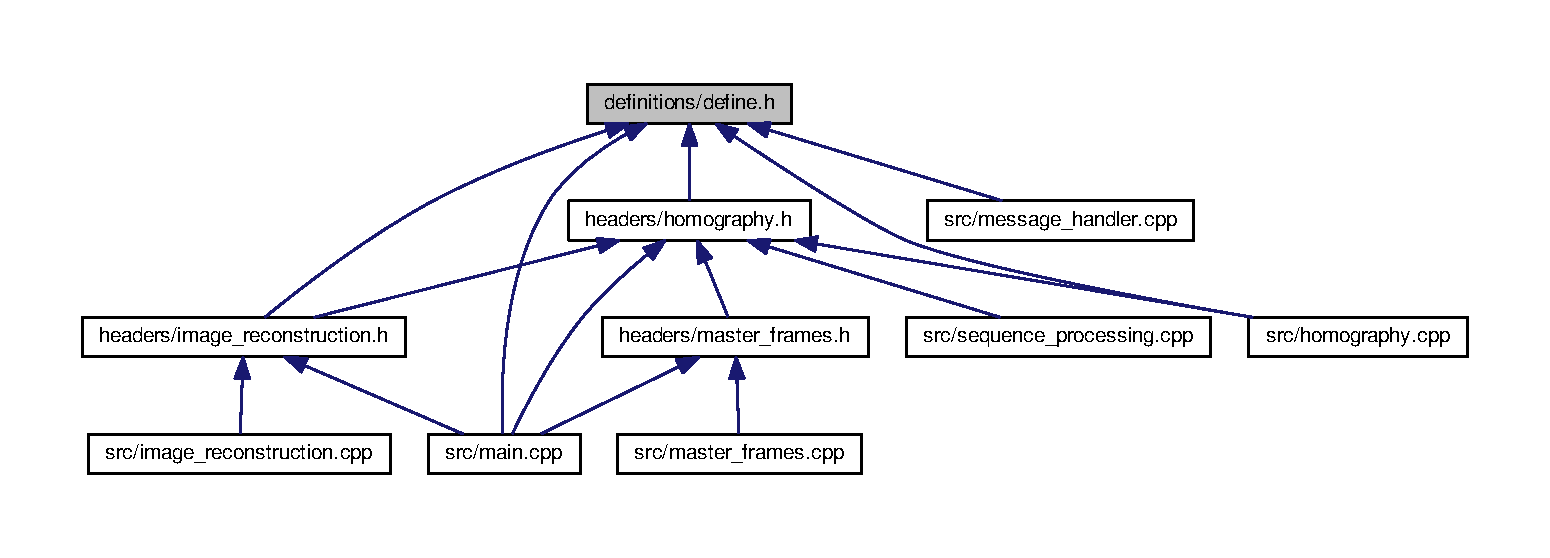
\includegraphics[width=350pt]{define_8h__dep__incl}
\end{center}
\end{figure}
\subsection*{Macros}
\begin{DoxyCompactItemize}
\item 
\#define \hyperlink{define_8h_a13198beec126efc77778680220fb4a15}{V\+I\+EW}~1 /$\ast$true$\ast$/    /$\ast$false$\ast$/
\begin{DoxyCompactList}\small\item\em Show images for each step of processing in a window called \textquotesingle{}Homography\textquotesingle{}. \end{DoxyCompactList}\item 
\#define \hyperlink{define_8h_a8290919fd7f022a7671a9c8ab642514b}{V\+I\+E\+W\+\_\+\+D\+E\+L\+AY}~0
\begin{DoxyCompactList}\small\item\em Show images for each step of processing in a window called \textquotesingle{}Homography\textquotesingle{}. \end{DoxyCompactList}\item 
\#define \hyperlink{define_8h_a4e7a6f58664fd0a43e3076399b98f08c}{F\+R\+A\+M\+E\+\_\+\+N\+U\+M\+B\+E\+R\+\_\+\+R\+E\+S\+U\+LT}~0 /$\ast$true$\ast$/    /$\ast$false$\ast$/
\begin{DoxyCompactList}\small\item\em Print the frame number in the images before save it. \end{DoxyCompactList}\item 
\#define \hyperlink{define_8h_a2c78c39688292c571d5953d7e9804ec5}{D\+E\+B\+U\+G\+\_\+\+I\+N\+T\+E\+R\+M\+E\+D\+I\+A\+T\+E\+\_\+\+F\+R\+A\+ME}~0 /$\ast$true$\ast$/    /$\ast$false$\ast$/
\begin{DoxyCompactList}\small\item\em Print variable values for each step of processing in the main cpp file. \end{DoxyCompactList}\item 
\#define \hyperlink{define_8h_a9b1ee3f8ba0f8b2838f1cf24c44519f4}{D\+E\+B\+U\+G\+\_\+\+F\+R\+A\+M\+E\+\_\+\+S\+T\+A\+T\+US}~1 /$\ast$true$\ast$/    /$\ast$false$\ast$/
\begin{DoxyCompactList}\small\item\em Print variable values for each step of processing in the main cpp file. \end{DoxyCompactList}\item 
\#define \hyperlink{define_8h_a9f0d78e00ea067275e3a1e8a0b2a1baa}{D\+E\+B\+U\+G\+\_\+\+H\+O\+M\+O\+G\+R\+A\+P\+HY}~0 /$\ast$true$\ast$/    /$\ast$false$\ast$/
\begin{DoxyCompactList}\small\item\em Print variable values for each step of processing in the homography cpp file. \end{DoxyCompactList}\item 
\#define \hyperlink{define_8h_ad9ad2864f6a3064acd18b4aac440108d}{D\+E\+B\+U\+G\+\_\+\+R\+E\+C\+O\+N\+S\+T\+R\+U\+C\+T\+I\+ON}~0 /$\ast$true$\ast$/    /$\ast$false$\ast$/
\begin{DoxyCompactList}\small\item\em Print variable values for each step of processing in the image\+\_\+reconstruciton cpp file. \end{DoxyCompactList}\item 
\#define \hyperlink{define_8h_aa55124c9e7cbfdf5b234e4f8128618e8}{M\+I\+N\+\_\+\+N\+U\+M\+B\+E\+R\+\_\+\+O\+F\+\_\+\+G\+O\+O\+D\+\_\+\+M\+A\+T\+C\+H\+ES}~50
\begin{DoxyCompactList}\small\item\em Minimum number of good matches to calcule the homography matrix. \end{DoxyCompactList}\item 
\#define \hyperlink{define_8h_a249638630837bda97ebb266001f43181}{M\+A\+X\+I\+M\+U\+M\+\_\+\+A\+R\+E\+A\+\_\+\+A\+L\+L\+O\+W\+ED}~0.\+001d
\begin{DoxyCompactList}\small\item\em Maximum area allowed to check if an image need to continue on being reconstructed. \end{DoxyCompactList}\item 
\#define \hyperlink{define_8h_afacb15ef807794c331301421eabbf6c9}{N\+U\+M\+\_\+\+M\+A\+X\+\_\+\+I\+M\+A\+G\+E\+S\+\_\+\+T\+O\+\_\+\+R\+E\+C\+O\+N\+S\+T\+R\+U\+CT}~30
\begin{DoxyCompactList}\small\item\em Number maximum of images that could be used to reconstruct a image in the \hyperlink{image__reconstruction_8cpp}{image\+\_\+reconstruction.\+cpp}. \end{DoxyCompactList}\item 
\#define \hyperlink{define_8h_aa3f3943af5fdd5551c55e5ae7e9a6abc}{M\+I\+N\+\_\+\+H\+E\+S\+S\+I\+AN}~400
\begin{DoxyCompactList}\small\item\em The S\+U\+RF Hessian minimum threshold. \end{DoxyCompactList}\item 
\#define \hyperlink{define_8h_a72de703228ed5e9def19a41d75583717}{M\+A\+T\+C\+H\+E\+S\+\_\+\+T\+H\+R\+E\+S\+H\+O\+L\+D\+\_\+\+F\+A\+C\+T\+OR}~3
\begin{DoxyCompactList}\small\item\em Multiplier to the minimum distance from descriptors to set a threshold in matches search. \end{DoxyCompactList}\item 
\#define \hyperlink{define_8h_aa3058a26bcaae9fc46b648e30e2031a0}{C\+R\+O\+P\+\_\+\+P\+O\+R\+T\+I\+ON}~0.\+05f
\begin{DoxyCompactList}\small\item\em The percentage of the original image that can be lost. \end{DoxyCompactList}\item 
\#define \hyperlink{define_8h_ad0321d6454b40d9bff133bb1069e2a75}{D\+R\+O\+P\+\_\+\+P\+O\+R\+T\+I\+ON}~0.\+2f
\begin{DoxyCompactList}\small\item\em The percentage of the original image that can be lost. \end{DoxyCompactList}\item 
\#define \hyperlink{define_8h_a4a206f0b77a48c47af486acc3d3cf1be}{M\+A\+X\+\_\+\+D\+R\+O\+P\+\_\+\+A\+T\+T\+E\+M\+P\+TS}~3
\begin{DoxyCompactList}\small\item\em Max number of drops if smaller than the drop area. \end{DoxyCompactList}\item 
\#define \hyperlink{define_8h_aa9342e72f75f6fb967145d9ac545a040}{M\+A\+X\+\_\+\+S\+K\+IP}~100
\begin{DoxyCompactList}\small\item\em Max number of frames skip from any frame. \end{DoxyCompactList}\end{DoxyCompactItemize}


\subsection{Detailed Description}
Macros used in the code relate with debug/view flags and usual values. 



\subsection{Macro Definition Documentation}
\index{define.\+h@{define.\+h}!C\+R\+O\+P\+\_\+\+P\+O\+R\+T\+I\+ON@{C\+R\+O\+P\+\_\+\+P\+O\+R\+T\+I\+ON}}
\index{C\+R\+O\+P\+\_\+\+P\+O\+R\+T\+I\+ON@{C\+R\+O\+P\+\_\+\+P\+O\+R\+T\+I\+ON}!define.\+h@{define.\+h}}
\subsubsection[{\texorpdfstring{C\+R\+O\+P\+\_\+\+P\+O\+R\+T\+I\+ON}{CROP\_PORTION}}]{\setlength{\rightskip}{0pt plus 5cm}\#define C\+R\+O\+P\+\_\+\+P\+O\+R\+T\+I\+ON~0.\+05f}\hypertarget{define_8h_aa3058a26bcaae9fc46b648e30e2031a0}{}\label{define_8h_aa3058a26bcaae9fc46b648e30e2031a0}


The percentage of the original image that can be lost. 

\index{define.\+h@{define.\+h}!D\+E\+B\+U\+G\+\_\+\+F\+R\+A\+M\+E\+\_\+\+S\+T\+A\+T\+US@{D\+E\+B\+U\+G\+\_\+\+F\+R\+A\+M\+E\+\_\+\+S\+T\+A\+T\+US}}
\index{D\+E\+B\+U\+G\+\_\+\+F\+R\+A\+M\+E\+\_\+\+S\+T\+A\+T\+US@{D\+E\+B\+U\+G\+\_\+\+F\+R\+A\+M\+E\+\_\+\+S\+T\+A\+T\+US}!define.\+h@{define.\+h}}
\subsubsection[{\texorpdfstring{D\+E\+B\+U\+G\+\_\+\+F\+R\+A\+M\+E\+\_\+\+S\+T\+A\+T\+US}{DEBUG\_FRAME\_STATUS}}]{\setlength{\rightskip}{0pt plus 5cm}\#define D\+E\+B\+U\+G\+\_\+\+F\+R\+A\+M\+E\+\_\+\+S\+T\+A\+T\+US~1 /$\ast$true$\ast$/    /$\ast$false$\ast$/}\hypertarget{define_8h_a9b1ee3f8ba0f8b2838f1cf24c44519f4}{}\label{define_8h_a9b1ee3f8ba0f8b2838f1cf24c44519f4}


Print variable values for each step of processing in the main cpp file. 

\index{define.\+h@{define.\+h}!D\+E\+B\+U\+G\+\_\+\+H\+O\+M\+O\+G\+R\+A\+P\+HY@{D\+E\+B\+U\+G\+\_\+\+H\+O\+M\+O\+G\+R\+A\+P\+HY}}
\index{D\+E\+B\+U\+G\+\_\+\+H\+O\+M\+O\+G\+R\+A\+P\+HY@{D\+E\+B\+U\+G\+\_\+\+H\+O\+M\+O\+G\+R\+A\+P\+HY}!define.\+h@{define.\+h}}
\subsubsection[{\texorpdfstring{D\+E\+B\+U\+G\+\_\+\+H\+O\+M\+O\+G\+R\+A\+P\+HY}{DEBUG\_HOMOGRAPHY}}]{\setlength{\rightskip}{0pt plus 5cm}\#define D\+E\+B\+U\+G\+\_\+\+H\+O\+M\+O\+G\+R\+A\+P\+HY~0 /$\ast$true$\ast$/    /$\ast$false$\ast$/}\hypertarget{define_8h_a9f0d78e00ea067275e3a1e8a0b2a1baa}{}\label{define_8h_a9f0d78e00ea067275e3a1e8a0b2a1baa}


Print variable values for each step of processing in the homography cpp file. 

\index{define.\+h@{define.\+h}!D\+E\+B\+U\+G\+\_\+\+I\+N\+T\+E\+R\+M\+E\+D\+I\+A\+T\+E\+\_\+\+F\+R\+A\+ME@{D\+E\+B\+U\+G\+\_\+\+I\+N\+T\+E\+R\+M\+E\+D\+I\+A\+T\+E\+\_\+\+F\+R\+A\+ME}}
\index{D\+E\+B\+U\+G\+\_\+\+I\+N\+T\+E\+R\+M\+E\+D\+I\+A\+T\+E\+\_\+\+F\+R\+A\+ME@{D\+E\+B\+U\+G\+\_\+\+I\+N\+T\+E\+R\+M\+E\+D\+I\+A\+T\+E\+\_\+\+F\+R\+A\+ME}!define.\+h@{define.\+h}}
\subsubsection[{\texorpdfstring{D\+E\+B\+U\+G\+\_\+\+I\+N\+T\+E\+R\+M\+E\+D\+I\+A\+T\+E\+\_\+\+F\+R\+A\+ME}{DEBUG\_INTERMEDIATE\_FRAME}}]{\setlength{\rightskip}{0pt plus 5cm}\#define D\+E\+B\+U\+G\+\_\+\+I\+N\+T\+E\+R\+M\+E\+D\+I\+A\+T\+E\+\_\+\+F\+R\+A\+ME~0 /$\ast$true$\ast$/    /$\ast$false$\ast$/}\hypertarget{define_8h_a2c78c39688292c571d5953d7e9804ec5}{}\label{define_8h_a2c78c39688292c571d5953d7e9804ec5}


Print variable values for each step of processing in the main cpp file. 

\index{define.\+h@{define.\+h}!D\+E\+B\+U\+G\+\_\+\+R\+E\+C\+O\+N\+S\+T\+R\+U\+C\+T\+I\+ON@{D\+E\+B\+U\+G\+\_\+\+R\+E\+C\+O\+N\+S\+T\+R\+U\+C\+T\+I\+ON}}
\index{D\+E\+B\+U\+G\+\_\+\+R\+E\+C\+O\+N\+S\+T\+R\+U\+C\+T\+I\+ON@{D\+E\+B\+U\+G\+\_\+\+R\+E\+C\+O\+N\+S\+T\+R\+U\+C\+T\+I\+ON}!define.\+h@{define.\+h}}
\subsubsection[{\texorpdfstring{D\+E\+B\+U\+G\+\_\+\+R\+E\+C\+O\+N\+S\+T\+R\+U\+C\+T\+I\+ON}{DEBUG\_RECONSTRUCTION}}]{\setlength{\rightskip}{0pt plus 5cm}\#define D\+E\+B\+U\+G\+\_\+\+R\+E\+C\+O\+N\+S\+T\+R\+U\+C\+T\+I\+ON~0 /$\ast$true$\ast$/    /$\ast$false$\ast$/}\hypertarget{define_8h_ad9ad2864f6a3064acd18b4aac440108d}{}\label{define_8h_ad9ad2864f6a3064acd18b4aac440108d}


Print variable values for each step of processing in the image\+\_\+reconstruciton cpp file. 

\index{define.\+h@{define.\+h}!D\+R\+O\+P\+\_\+\+P\+O\+R\+T\+I\+ON@{D\+R\+O\+P\+\_\+\+P\+O\+R\+T\+I\+ON}}
\index{D\+R\+O\+P\+\_\+\+P\+O\+R\+T\+I\+ON@{D\+R\+O\+P\+\_\+\+P\+O\+R\+T\+I\+ON}!define.\+h@{define.\+h}}
\subsubsection[{\texorpdfstring{D\+R\+O\+P\+\_\+\+P\+O\+R\+T\+I\+ON}{DROP\_PORTION}}]{\setlength{\rightskip}{0pt plus 5cm}\#define D\+R\+O\+P\+\_\+\+P\+O\+R\+T\+I\+ON~0.\+2f}\hypertarget{define_8h_ad0321d6454b40d9bff133bb1069e2a75}{}\label{define_8h_ad0321d6454b40d9bff133bb1069e2a75}


The percentage of the original image that can be lost. 

\index{define.\+h@{define.\+h}!F\+R\+A\+M\+E\+\_\+\+N\+U\+M\+B\+E\+R\+\_\+\+R\+E\+S\+U\+LT@{F\+R\+A\+M\+E\+\_\+\+N\+U\+M\+B\+E\+R\+\_\+\+R\+E\+S\+U\+LT}}
\index{F\+R\+A\+M\+E\+\_\+\+N\+U\+M\+B\+E\+R\+\_\+\+R\+E\+S\+U\+LT@{F\+R\+A\+M\+E\+\_\+\+N\+U\+M\+B\+E\+R\+\_\+\+R\+E\+S\+U\+LT}!define.\+h@{define.\+h}}
\subsubsection[{\texorpdfstring{F\+R\+A\+M\+E\+\_\+\+N\+U\+M\+B\+E\+R\+\_\+\+R\+E\+S\+U\+LT}{FRAME\_NUMBER\_RESULT}}]{\setlength{\rightskip}{0pt plus 5cm}\#define F\+R\+A\+M\+E\+\_\+\+N\+U\+M\+B\+E\+R\+\_\+\+R\+E\+S\+U\+LT~0 /$\ast$true$\ast$/    /$\ast$false$\ast$/}\hypertarget{define_8h_a4e7a6f58664fd0a43e3076399b98f08c}{}\label{define_8h_a4e7a6f58664fd0a43e3076399b98f08c}


Print the frame number in the images before save it. 

\index{define.\+h@{define.\+h}!M\+A\+T\+C\+H\+E\+S\+\_\+\+T\+H\+R\+E\+S\+H\+O\+L\+D\+\_\+\+F\+A\+C\+T\+OR@{M\+A\+T\+C\+H\+E\+S\+\_\+\+T\+H\+R\+E\+S\+H\+O\+L\+D\+\_\+\+F\+A\+C\+T\+OR}}
\index{M\+A\+T\+C\+H\+E\+S\+\_\+\+T\+H\+R\+E\+S\+H\+O\+L\+D\+\_\+\+F\+A\+C\+T\+OR@{M\+A\+T\+C\+H\+E\+S\+\_\+\+T\+H\+R\+E\+S\+H\+O\+L\+D\+\_\+\+F\+A\+C\+T\+OR}!define.\+h@{define.\+h}}
\subsubsection[{\texorpdfstring{M\+A\+T\+C\+H\+E\+S\+\_\+\+T\+H\+R\+E\+S\+H\+O\+L\+D\+\_\+\+F\+A\+C\+T\+OR}{MATCHES\_THRESHOLD\_FACTOR}}]{\setlength{\rightskip}{0pt plus 5cm}\#define M\+A\+T\+C\+H\+E\+S\+\_\+\+T\+H\+R\+E\+S\+H\+O\+L\+D\+\_\+\+F\+A\+C\+T\+OR~3}\hypertarget{define_8h_a72de703228ed5e9def19a41d75583717}{}\label{define_8h_a72de703228ed5e9def19a41d75583717}


Multiplier to the minimum distance from descriptors to set a threshold in matches search. 

\index{define.\+h@{define.\+h}!M\+A\+X\+\_\+\+D\+R\+O\+P\+\_\+\+A\+T\+T\+E\+M\+P\+TS@{M\+A\+X\+\_\+\+D\+R\+O\+P\+\_\+\+A\+T\+T\+E\+M\+P\+TS}}
\index{M\+A\+X\+\_\+\+D\+R\+O\+P\+\_\+\+A\+T\+T\+E\+M\+P\+TS@{M\+A\+X\+\_\+\+D\+R\+O\+P\+\_\+\+A\+T\+T\+E\+M\+P\+TS}!define.\+h@{define.\+h}}
\subsubsection[{\texorpdfstring{M\+A\+X\+\_\+\+D\+R\+O\+P\+\_\+\+A\+T\+T\+E\+M\+P\+TS}{MAX\_DROP\_ATTEMPTS}}]{\setlength{\rightskip}{0pt plus 5cm}\#define M\+A\+X\+\_\+\+D\+R\+O\+P\+\_\+\+A\+T\+T\+E\+M\+P\+TS~3}\hypertarget{define_8h_a4a206f0b77a48c47af486acc3d3cf1be}{}\label{define_8h_a4a206f0b77a48c47af486acc3d3cf1be}


Max number of drops if smaller than the drop area. 

\index{define.\+h@{define.\+h}!M\+A\+X\+\_\+\+S\+K\+IP@{M\+A\+X\+\_\+\+S\+K\+IP}}
\index{M\+A\+X\+\_\+\+S\+K\+IP@{M\+A\+X\+\_\+\+S\+K\+IP}!define.\+h@{define.\+h}}
\subsubsection[{\texorpdfstring{M\+A\+X\+\_\+\+S\+K\+IP}{MAX\_SKIP}}]{\setlength{\rightskip}{0pt plus 5cm}\#define M\+A\+X\+\_\+\+S\+K\+IP~100}\hypertarget{define_8h_aa9342e72f75f6fb967145d9ac545a040}{}\label{define_8h_aa9342e72f75f6fb967145d9ac545a040}


Max number of frames skip from any frame. 

Defined by the fast-\/forward algorithm. \index{define.\+h@{define.\+h}!M\+A\+X\+I\+M\+U\+M\+\_\+\+A\+R\+E\+A\+\_\+\+A\+L\+L\+O\+W\+ED@{M\+A\+X\+I\+M\+U\+M\+\_\+\+A\+R\+E\+A\+\_\+\+A\+L\+L\+O\+W\+ED}}
\index{M\+A\+X\+I\+M\+U\+M\+\_\+\+A\+R\+E\+A\+\_\+\+A\+L\+L\+O\+W\+ED@{M\+A\+X\+I\+M\+U\+M\+\_\+\+A\+R\+E\+A\+\_\+\+A\+L\+L\+O\+W\+ED}!define.\+h@{define.\+h}}
\subsubsection[{\texorpdfstring{M\+A\+X\+I\+M\+U\+M\+\_\+\+A\+R\+E\+A\+\_\+\+A\+L\+L\+O\+W\+ED}{MAXIMUM\_AREA\_ALLOWED}}]{\setlength{\rightskip}{0pt plus 5cm}\#define M\+A\+X\+I\+M\+U\+M\+\_\+\+A\+R\+E\+A\+\_\+\+A\+L\+L\+O\+W\+ED~0.\+001d}\hypertarget{define_8h_a249638630837bda97ebb266001f43181}{}\label{define_8h_a249638630837bda97ebb266001f43181}


Maximum area allowed to check if an image need to continue on being reconstructed. 

\index{define.\+h@{define.\+h}!M\+I\+N\+\_\+\+H\+E\+S\+S\+I\+AN@{M\+I\+N\+\_\+\+H\+E\+S\+S\+I\+AN}}
\index{M\+I\+N\+\_\+\+H\+E\+S\+S\+I\+AN@{M\+I\+N\+\_\+\+H\+E\+S\+S\+I\+AN}!define.\+h@{define.\+h}}
\subsubsection[{\texorpdfstring{M\+I\+N\+\_\+\+H\+E\+S\+S\+I\+AN}{MIN\_HESSIAN}}]{\setlength{\rightskip}{0pt plus 5cm}\#define M\+I\+N\+\_\+\+H\+E\+S\+S\+I\+AN~400}\hypertarget{define_8h_aa3f3943af5fdd5551c55e5ae7e9a6abc}{}\label{define_8h_aa3f3943af5fdd5551c55e5ae7e9a6abc}


The S\+U\+RF Hessian minimum threshold. 

\index{define.\+h@{define.\+h}!M\+I\+N\+\_\+\+N\+U\+M\+B\+E\+R\+\_\+\+O\+F\+\_\+\+G\+O\+O\+D\+\_\+\+M\+A\+T\+C\+H\+ES@{M\+I\+N\+\_\+\+N\+U\+M\+B\+E\+R\+\_\+\+O\+F\+\_\+\+G\+O\+O\+D\+\_\+\+M\+A\+T\+C\+H\+ES}}
\index{M\+I\+N\+\_\+\+N\+U\+M\+B\+E\+R\+\_\+\+O\+F\+\_\+\+G\+O\+O\+D\+\_\+\+M\+A\+T\+C\+H\+ES@{M\+I\+N\+\_\+\+N\+U\+M\+B\+E\+R\+\_\+\+O\+F\+\_\+\+G\+O\+O\+D\+\_\+\+M\+A\+T\+C\+H\+ES}!define.\+h@{define.\+h}}
\subsubsection[{\texorpdfstring{M\+I\+N\+\_\+\+N\+U\+M\+B\+E\+R\+\_\+\+O\+F\+\_\+\+G\+O\+O\+D\+\_\+\+M\+A\+T\+C\+H\+ES}{MIN\_NUMBER\_OF\_GOOD\_MATCHES}}]{\setlength{\rightskip}{0pt plus 5cm}\#define M\+I\+N\+\_\+\+N\+U\+M\+B\+E\+R\+\_\+\+O\+F\+\_\+\+G\+O\+O\+D\+\_\+\+M\+A\+T\+C\+H\+ES~50}\hypertarget{define_8h_aa55124c9e7cbfdf5b234e4f8128618e8}{}\label{define_8h_aa55124c9e7cbfdf5b234e4f8128618e8}


Minimum number of good matches to calcule the homography matrix. 

\index{define.\+h@{define.\+h}!N\+U\+M\+\_\+\+M\+A\+X\+\_\+\+I\+M\+A\+G\+E\+S\+\_\+\+T\+O\+\_\+\+R\+E\+C\+O\+N\+S\+T\+R\+U\+CT@{N\+U\+M\+\_\+\+M\+A\+X\+\_\+\+I\+M\+A\+G\+E\+S\+\_\+\+T\+O\+\_\+\+R\+E\+C\+O\+N\+S\+T\+R\+U\+CT}}
\index{N\+U\+M\+\_\+\+M\+A\+X\+\_\+\+I\+M\+A\+G\+E\+S\+\_\+\+T\+O\+\_\+\+R\+E\+C\+O\+N\+S\+T\+R\+U\+CT@{N\+U\+M\+\_\+\+M\+A\+X\+\_\+\+I\+M\+A\+G\+E\+S\+\_\+\+T\+O\+\_\+\+R\+E\+C\+O\+N\+S\+T\+R\+U\+CT}!define.\+h@{define.\+h}}
\subsubsection[{\texorpdfstring{N\+U\+M\+\_\+\+M\+A\+X\+\_\+\+I\+M\+A\+G\+E\+S\+\_\+\+T\+O\+\_\+\+R\+E\+C\+O\+N\+S\+T\+R\+U\+CT}{NUM\_MAX\_IMAGES\_TO\_RECONSTRUCT}}]{\setlength{\rightskip}{0pt plus 5cm}\#define N\+U\+M\+\_\+\+M\+A\+X\+\_\+\+I\+M\+A\+G\+E\+S\+\_\+\+T\+O\+\_\+\+R\+E\+C\+O\+N\+S\+T\+R\+U\+CT~30}\hypertarget{define_8h_afacb15ef807794c331301421eabbf6c9}{}\label{define_8h_afacb15ef807794c331301421eabbf6c9}


Number maximum of images that could be used to reconstruct a image in the \hyperlink{image__reconstruction_8cpp}{image\+\_\+reconstruction.\+cpp}. 

\index{define.\+h@{define.\+h}!V\+I\+EW@{V\+I\+EW}}
\index{V\+I\+EW@{V\+I\+EW}!define.\+h@{define.\+h}}
\subsubsection[{\texorpdfstring{V\+I\+EW}{VIEW}}]{\setlength{\rightskip}{0pt plus 5cm}\#define V\+I\+EW~1 /$\ast$true$\ast$/    /$\ast$false$\ast$/}\hypertarget{define_8h_a13198beec126efc77778680220fb4a15}{}\label{define_8h_a13198beec126efc77778680220fb4a15}


Show images for each step of processing in a window called \textquotesingle{}Homography\textquotesingle{}. 

\index{define.\+h@{define.\+h}!V\+I\+E\+W\+\_\+\+D\+E\+L\+AY@{V\+I\+E\+W\+\_\+\+D\+E\+L\+AY}}
\index{V\+I\+E\+W\+\_\+\+D\+E\+L\+AY@{V\+I\+E\+W\+\_\+\+D\+E\+L\+AY}!define.\+h@{define.\+h}}
\subsubsection[{\texorpdfstring{V\+I\+E\+W\+\_\+\+D\+E\+L\+AY}{VIEW\_DELAY}}]{\setlength{\rightskip}{0pt plus 5cm}\#define V\+I\+E\+W\+\_\+\+D\+E\+L\+AY~0}\hypertarget{define_8h_a8290919fd7f022a7671a9c8ab642514b}{}\label{define_8h_a8290919fd7f022a7671a9c8ab642514b}


Show images for each step of processing in a window called \textquotesingle{}Homography\textquotesingle{}. 


\hypertarget{experiment__struct_8h}{}\section{definitions/experiment\+\_\+struct.h File Reference}
\label{experiment__struct_8h}\index{definitions/experiment\+\_\+struct.\+h@{definitions/experiment\+\_\+struct.\+h}}


Fields declaration of the experiment settings.  


{\ttfamily \#include $<$stdio.\+h$>$}\\*
{\ttfamily \#include $<$string$>$}\\*
Include dependency graph for experiment\+\_\+struct.\+h\+:\nopagebreak
\begin{figure}[H]
\begin{center}
\leavevmode
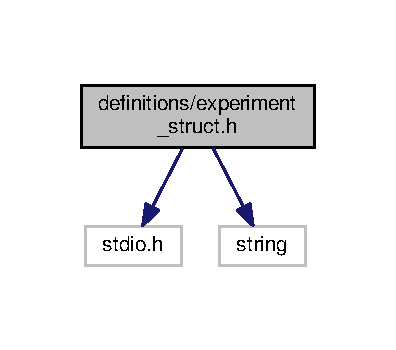
\includegraphics[width=190pt]{experiment__struct_8h__incl}
\end{center}
\end{figure}
This graph shows which files directly or indirectly include this file\+:\nopagebreak
\begin{figure}[H]
\begin{center}
\leavevmode
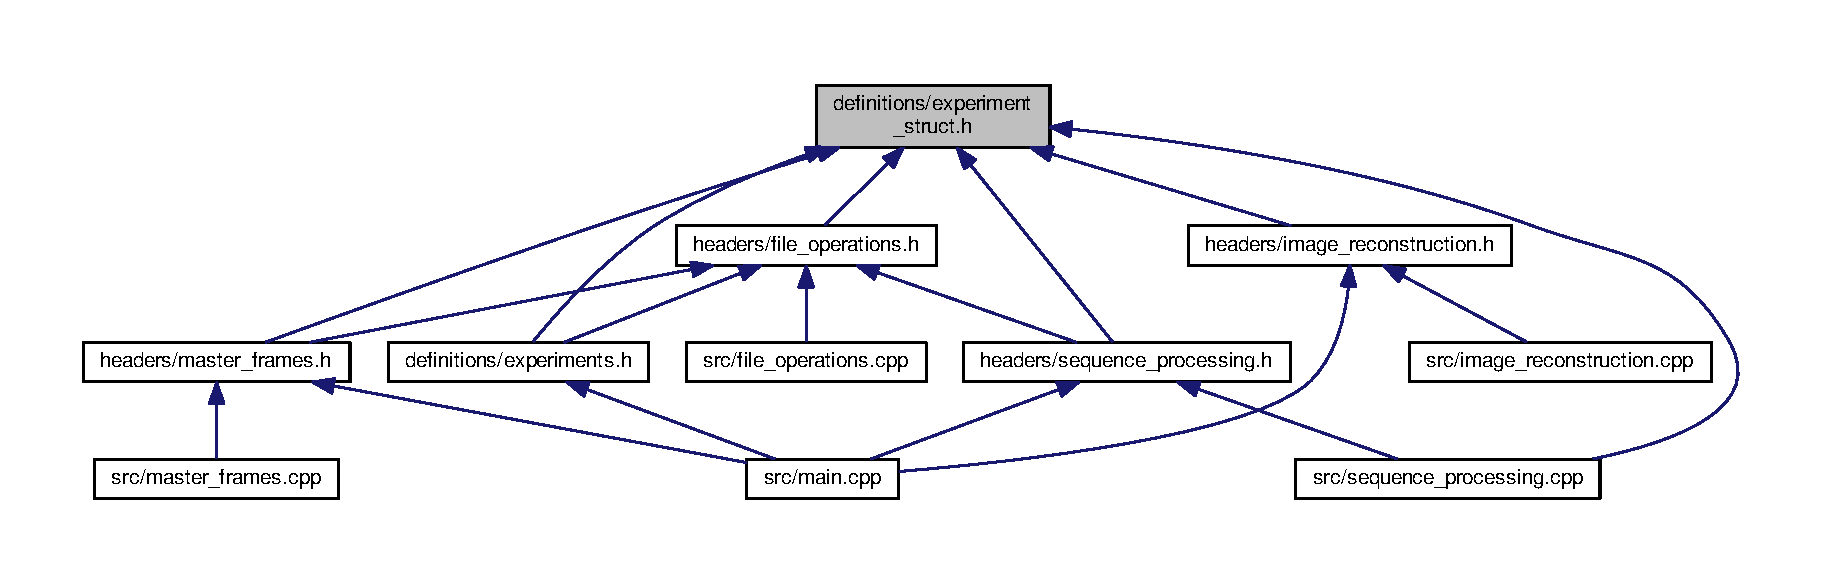
\includegraphics[width=350pt]{experiment__struct_8h__dep__incl}
\end{center}
\end{figure}
\subsection*{Classes}
\begin{DoxyCompactItemize}
\item 
struct \hyperlink{structEXPERIMENT}{E\+X\+P\+E\+R\+I\+M\+E\+NT}
\end{DoxyCompactItemize}


\subsection{Detailed Description}
Fields declaration of the experiment settings. 


\hypertarget{experiments_8h}{}\section{definitions/experiments.h File Reference}
\label{experiments_8h}\index{definitions/experiments.\+h@{definitions/experiments.\+h}}


Definitions of experiment settings.  


{\ttfamily \#include $<$stdio.\+h$>$}\\*
{\ttfamily \#include $<$stdlib.\+h$>$}\\*
{\ttfamily \#include $<$algorithm$>$}\\*
{\ttfamily \#include $<$string.\+h$>$}\\*
{\ttfamily \#include $<$unistd.\+h$>$}\\*
{\ttfamily \#include $<$opencv2/core/core.\+hpp$>$}\\*
{\ttfamily \#include \char`\"{}definitions/experiment\+\_\+struct.\+h\char`\"{}}\\*
{\ttfamily \#include \char`\"{}executables/execute\+\_\+commands.\+h\char`\"{}}\\*
{\ttfamily \#include \char`\"{}headers/file\+\_\+operations.\+h\char`\"{}}\\*
Include dependency graph for experiments.\+h\+:\nopagebreak
\begin{figure}[H]
\begin{center}
\leavevmode
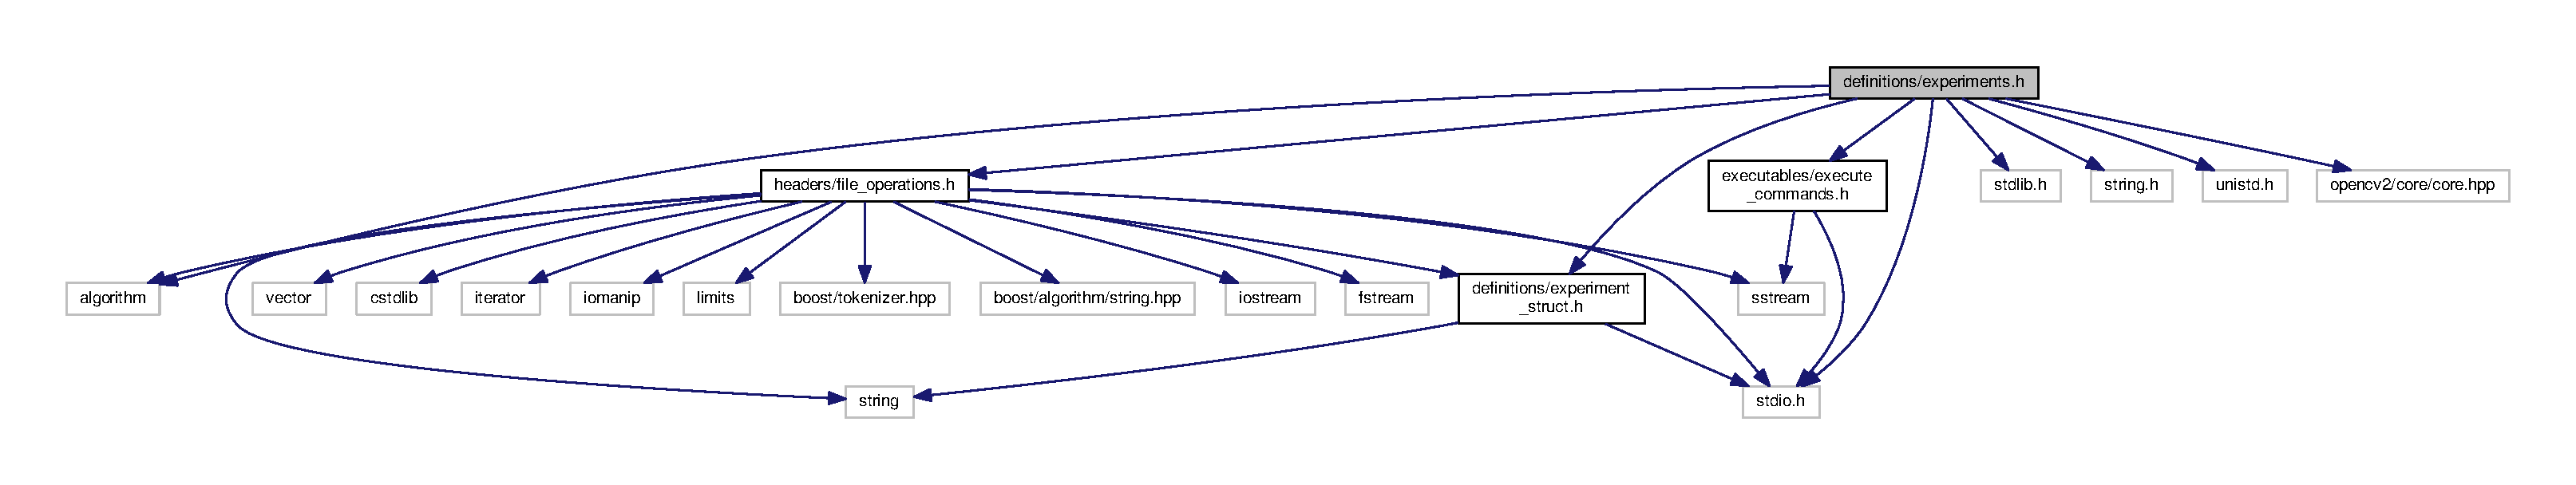
\includegraphics[width=350pt]{experiments_8h__incl}
\end{center}
\end{figure}
This graph shows which files directly or indirectly include this file\+:\nopagebreak
\begin{figure}[H]
\begin{center}
\leavevmode
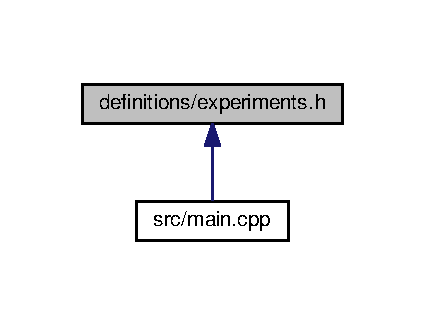
\includegraphics[width=204pt]{experiments_8h__dep__incl}
\end{center}
\end{figure}
\subsection*{Functions}
\begin{DoxyCompactItemize}
\item 
\hyperlink{structEXPERIMENT}{E\+X\+P\+E\+R\+I\+M\+E\+NT} \hyperlink{experiments_8h_ab209a6fbc3cd78cd0cbc131d71243709}{load\+\_\+experiments\+\_\+settings} (std\+::string settings\+Filename)
\end{DoxyCompactItemize}


\subsection{Detailed Description}
Definitions of experiment settings. 



\subsection{Function Documentation}
\index{experiments.\+h@{experiments.\+h}!load\+\_\+experiments\+\_\+settings@{load\+\_\+experiments\+\_\+settings}}
\index{load\+\_\+experiments\+\_\+settings@{load\+\_\+experiments\+\_\+settings}!experiments.\+h@{experiments.\+h}}
\subsubsection[{\texorpdfstring{load\+\_\+experiments\+\_\+settings(std\+::string settings\+Filename)}{load\_experiments\_settings(std::string settingsFilename)}}]{\setlength{\rightskip}{0pt plus 5cm}{\bf E\+X\+P\+E\+R\+I\+M\+E\+NT} load\+\_\+experiments\+\_\+settings (
\begin{DoxyParamCaption}
\item[{std\+::string}]{settings\+Filename}
\end{DoxyParamCaption}
)}\hypertarget{experiments_8h_ab209a6fbc3cd78cd0cbc131d71243709}{}\label{experiments_8h_ab209a6fbc3cd78cd0cbc131d71243709}
{\itshape std\+::string} {\bfseries video\+\_\+path\+:}Complete path to the video.

{\itshape std\+::string} {\bfseries output\+\_\+path\+:} Complete path to the folder where the results will be saved. It is important that the user have permission to write there.

{\itshape std\+::string} {\bfseries video\+\_\+name\+:} Filename of the video with extension.

{\itshape std\+::string} {\bfseries original\+\_\+video\+\_\+filename\+:} Complete path and filename of the original video.

{\itshape std\+::string} {\bfseries read\+\_\+masterframes\+\_\+filename\+:} Complete path and filename of the txt file with the selected master frames.

{\itshape std\+::string} {\bfseries selected\+\_\+frames\+\_\+filename\+:} Complete path and filename of the csv file with the selected master frames that was selected to create the reduced video.

{\itshape std\+::string} {\bfseries semantic\+\_\+costs\+\_\+filename\+:} Complete path and filename of the csv file with the semantic cost of the frame transitions.

{\itshape std\+::string} {\bfseries instability\+\_\+costs\+\_\+filename\+:} Complete path and filename of the csv file with the jitter costs of the transitions.

{\itshape std\+::string} {\bfseries optical\+\_\+flow\+\_\+filename\+:} Complete path and filename of the csv file with the optical flow calculated by Flow\+Net.

{\itshape int} {\bfseries segment\+Size\+:} Size of the segments where the master frames will be calculated. It needs to be a power of two (2, 4, 8, 16, ...).

{\itshape bool} {\bfseries save\+Master\+Frames\+In\+Disk\+:} After calculte the master frames, do you want to save it in a file? After you can load it directly withou calculate again

{\itshape bool} {\bfseries save\+Video\+In\+Disk\+:} Save stabilized video in Disk.

{\itshape bool} {\bfseries running\+Parallel\+:} Running the master frames selection in parallel processors. 
\hypertarget{doc__mainpage_8md}{}\section{doc/doc\+\_\+mainpage.md File Reference}
\label{doc__mainpage_8md}\index{doc/doc\+\_\+mainpage.\+md@{doc/doc\+\_\+mainpage.\+md}}

\hypertarget{execute__commands_8h}{}\section{executables/execute\+\_\+commands.h File Reference}
\label{execute__commands_8h}\index{executables/execute\+\_\+commands.\+h@{executables/execute\+\_\+commands.\+h}}


Macro with specific codes.  


{\ttfamily \#include $<$sstream$>$}\\*
{\ttfamily \#include $<$stdio.\+h$>$}\\*
Include dependency graph for execute\+\_\+commands.\+h\+:\nopagebreak
\begin{figure}[H]
\begin{center}
\leavevmode
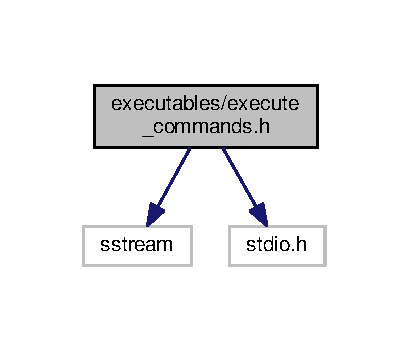
\includegraphics[width=196pt]{execute__commands_8h__incl}
\end{center}
\end{figure}
This graph shows which files directly or indirectly include this file\+:\nopagebreak
\begin{figure}[H]
\begin{center}
\leavevmode
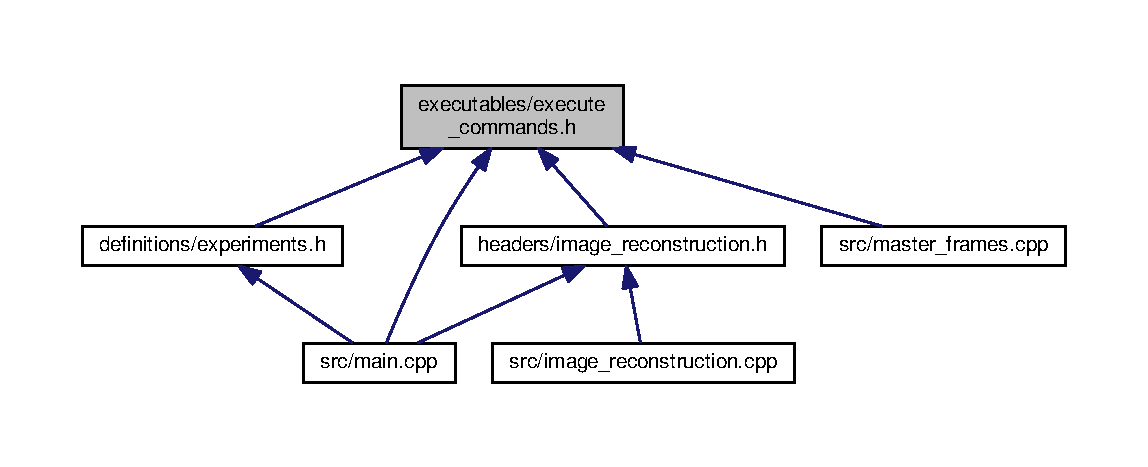
\includegraphics[width=350pt]{execute__commands_8h__dep__incl}
\end{center}
\end{figure}
\subsection*{Macros}
\begin{DoxyCompactItemize}
\item 
\#define \hyperlink{execute__commands_8h_a53f1ccb877151aca373061692ce50bf8}{E\+X\+E\+C\+U\+T\+E\+\_\+\+I\+N\+FO}
\item 
\#define \hyperlink{execute__commands_8h_ab0b8db66688c5a311dc396f1104a563a}{E\+X\+E\+C\+U\+T\+E\+\_\+\+E\+X\+P\+E\+R\+I\+M\+E\+N\+T\+\_\+\+ID}
\item 
\#define \hyperlink{execute__commands_8h_a860f56fe1fc9e103945671f4b7cca16a}{E\+X\+E\+C\+U\+T\+E\+\_\+\+V\+I\+EW}
\item 
\#define \hyperlink{execute__commands_8h_a633ebeb13695e1b87a2c65f53df0c836}{E\+X\+E\+C\+U\+T\+E\+\_\+\+I\+M\+A\+G\+E\+\_\+\+S\+T\+U\+F\+FS}(string\+\_\+length,  frame)
\item 
\#define \hyperlink{execute__commands_8h_a815c984330fd59b9a693211960320727}{E\+X\+E\+C\+U\+T\+E\+\_\+\+I\+M\+A\+G\+E\+\_\+\+R\+E\+C\+O\+N\+S\+T\+R\+U\+C\+T\+I\+ON}
\item 
\#define \hyperlink{execute__commands_8h_a44bd5e86ab21468210dbb71424eda082}{E\+X\+E\+C\+U\+T\+E\+\_\+\+I\+M\+A\+G\+E\+\_\+\+C\+O\+N\+D\+I\+T\+I\+O\+N\+A\+L\+\_\+\+A\+C\+T\+I\+O\+NS}
\item 
\#define \hyperlink{execute__commands_8h_a0d2f37137ee1fd6ff4a0ef803849dd63}{S\+S\+TR}(x)
\end{DoxyCompactItemize}


\subsection{Detailed Description}
Macro with specific codes. 



\subsection{Macro Definition Documentation}
\index{execute\+\_\+commands.\+h@{execute\+\_\+commands.\+h}!E\+X\+E\+C\+U\+T\+E\+\_\+\+E\+X\+P\+E\+R\+I\+M\+E\+N\+T\+\_\+\+ID@{E\+X\+E\+C\+U\+T\+E\+\_\+\+E\+X\+P\+E\+R\+I\+M\+E\+N\+T\+\_\+\+ID}}
\index{E\+X\+E\+C\+U\+T\+E\+\_\+\+E\+X\+P\+E\+R\+I\+M\+E\+N\+T\+\_\+\+ID@{E\+X\+E\+C\+U\+T\+E\+\_\+\+E\+X\+P\+E\+R\+I\+M\+E\+N\+T\+\_\+\+ID}!execute\+\_\+commands.\+h@{execute\+\_\+commands.\+h}}
\subsubsection[{\texorpdfstring{E\+X\+E\+C\+U\+T\+E\+\_\+\+E\+X\+P\+E\+R\+I\+M\+E\+N\+T\+\_\+\+ID}{EXECUTE\_EXPERIMENT\_ID}}]{\setlength{\rightskip}{0pt plus 5cm}\#define E\+X\+E\+C\+U\+T\+E\+\_\+\+E\+X\+P\+E\+R\+I\+M\+E\+N\+T\+\_\+\+ID}\hypertarget{execute__commands_8h_ab0b8db66688c5a311dc396f1104a563a}{}\label{execute__commands_8h_ab0b8db66688c5a311dc396f1104a563a}
{\bfseries Value\+:}
\begin{DoxyCode}
std::cout << std::endl \(\backslash\)
            << \textcolor{stringliteral}{" Running exepriment: "} << argv[1] << \textcolor{stringliteral}{" | Experiment ID: "} << 
      \hyperlink{main_8cpp_a9f5a81402e170475690f371d55cbe623}{experiment\_settings}.\hyperlink{structEXPERIMENT_af59b6805fe0851b89d1300849db794e4}{id} << std::endl \(\backslash\)
            << std::endl; \(\backslash\)
\end{DoxyCode}
\index{execute\+\_\+commands.\+h@{execute\+\_\+commands.\+h}!E\+X\+E\+C\+U\+T\+E\+\_\+\+I\+M\+A\+G\+E\+\_\+\+C\+O\+N\+D\+I\+T\+I\+O\+N\+A\+L\+\_\+\+A\+C\+T\+I\+O\+NS@{E\+X\+E\+C\+U\+T\+E\+\_\+\+I\+M\+A\+G\+E\+\_\+\+C\+O\+N\+D\+I\+T\+I\+O\+N\+A\+L\+\_\+\+A\+C\+T\+I\+O\+NS}}
\index{E\+X\+E\+C\+U\+T\+E\+\_\+\+I\+M\+A\+G\+E\+\_\+\+C\+O\+N\+D\+I\+T\+I\+O\+N\+A\+L\+\_\+\+A\+C\+T\+I\+O\+NS@{E\+X\+E\+C\+U\+T\+E\+\_\+\+I\+M\+A\+G\+E\+\_\+\+C\+O\+N\+D\+I\+T\+I\+O\+N\+A\+L\+\_\+\+A\+C\+T\+I\+O\+NS}!execute\+\_\+commands.\+h@{execute\+\_\+commands.\+h}}
\subsubsection[{\texorpdfstring{E\+X\+E\+C\+U\+T\+E\+\_\+\+I\+M\+A\+G\+E\+\_\+\+C\+O\+N\+D\+I\+T\+I\+O\+N\+A\+L\+\_\+\+A\+C\+T\+I\+O\+NS}{EXECUTE\_IMAGE\_CONDITIONAL\_ACTIONS}}]{\setlength{\rightskip}{0pt plus 5cm}\#define E\+X\+E\+C\+U\+T\+E\+\_\+\+I\+M\+A\+G\+E\+\_\+\+C\+O\+N\+D\+I\+T\+I\+O\+N\+A\+L\+\_\+\+A\+C\+T\+I\+O\+NS}\hypertarget{execute__commands_8h_a44bd5e86ab21468210dbb71424eda082}{}\label{execute__commands_8h_a44bd5e86ab21468210dbb71424eda082}
{\bfseries Value\+:}
\begin{DoxyCode}
\textcolor{keywordflow}{if} ( \hyperlink{homography_8h_a94196b6d4321a287adf2b3051a5fad83}{getAreaRatio}( current\_frame , homography\_matrix , crop\_area ) > 
      \hyperlink{define_8h_a249638630837bda97ebb266001f43181}{MAXIMUM\_AREA\_ALLOWED} ) \{ \(\backslash\)
    if ( \hyperlink{homography_8h_a94196b6d4321a287adf2b3051a5fad83}{getAreaRatio}( current\_frame , homography\_matrix , drop\_area ) > 
      \hyperlink{define_8h_a249638630837bda97ebb266001f43181}{MAXIMUM\_AREA\_ALLOWED} ) \{ \(\backslash\)
        log\_file << \textcolor{stringliteral}{" Frame : "} << \hyperlink{execute__commands_8h_a0d2f37137ee1fd6ff4a0ef803849dd63}{SSTR} ( std::setfill(\textcolor{charliteral}{'0'}) << std::setw(
      \hyperlink{main_8cpp_a6725a70b6f47b0c88de524c592b70856}{log\_number\_length}) << i ) << \textcolor{stringliteral}{" | [D] Dropped, a new one will be selected in the original
       video."} << std::endl; \(\backslash\)
        if ( \hyperlink{define_8h_a9b1ee3f8ba0f8b2838f1cf24c44519f4}{DEBUG\_FRAME\_STATUS} ) \(\backslash\)
            std::cout << \textcolor{stringliteral}{" i : "} << \hyperlink{execute__commands_8h_a0d2f37137ee1fd6ff4a0ef803849dd63}{SSTR} ( std::setfill(\textcolor{charliteral}{'0'}) << std::setw(
      \hyperlink{main_8cpp_a6725a70b6f47b0c88de524c592b70856}{log\_number\_length}) << i ) << \textcolor{stringliteral}{" | [D] Dropped, a new one will be selected in the original
       video."} << std::endl; \(\backslash\)
        num\_of\_dropped\_frames++; \(\backslash\)
    \} \textcolor{keywordflow}{else} \{ \(\backslash\)
        log\_file << \textcolor{stringliteral}{" Frame : "} << \hyperlink{execute__commands_8h_a0d2f37137ee1fd6ff4a0ef803849dd63}{SSTR} ( std::setfill(\textcolor{charliteral}{'0'}) << std::setw(
      \hyperlink{main_8cpp_a6725a70b6f47b0c88de524c592b70856}{log\_number\_length}) << i ) << \textcolor{stringliteral}{" | [R] Reconstructed using the original video."} << std::endl
      ; \(\backslash\)
        if ( \hyperlink{define_8h_a9b1ee3f8ba0f8b2838f1cf24c44519f4}{DEBUG\_FRAME\_STATUS} ) \(\backslash\)
            std::cout << \textcolor{stringliteral}{" i : "} << \hyperlink{execute__commands_8h_a0d2f37137ee1fd6ff4a0ef803849dd63}{SSTR} ( std::setfill(\textcolor{charliteral}{'0'}) << std::setw(
      \hyperlink{main_8cpp_a6725a70b6f47b0c88de524c592b70856}{log\_number\_length}) << i ) << \textcolor{stringliteral}{" | [R] Reconstructed using the original video."} << std::endl
      ; \(\backslash\)
        EXECUTE\_IMAGE\_RECONSTRUCTION \(\backslash\)
    \} \(\backslash\)
\} \textcolor{keywordflow}{else} \{ \(\backslash\)
    log\_file << \textcolor{stringliteral}{" Frame : "} << \hyperlink{execute__commands_8h_a0d2f37137ee1fd6ff4a0ef803849dd63}{SSTR} ( std::setfill(\textcolor{charliteral}{'0'}) << std::setw(
      \hyperlink{main_8cpp_a6725a70b6f47b0c88de524c592b70856}{log\_number\_length}) << i ) << \textcolor{stringliteral}{" | [K] Kept."} << std::endl; \(\backslash\)
    if ( \hyperlink{define_8h_a9b1ee3f8ba0f8b2838f1cf24c44519f4}{DEBUG\_FRAME\_STATUS} ) \(\backslash\)
        std::cout << \textcolor{stringliteral}{" i : "} << \hyperlink{execute__commands_8h_a0d2f37137ee1fd6ff4a0ef803849dd63}{SSTR} ( std::setfill(\textcolor{charliteral}{'0'}) << std::setw(
      \hyperlink{main_8cpp_a6725a70b6f47b0c88de524c592b70856}{log\_number\_length}) << i ) << \textcolor{stringliteral}{" | [K] Kept."} << std::endl; \(\backslash\)
    num\_of\_good\_frames++; \(\backslash\)
\}
\end{DoxyCode}
\index{execute\+\_\+commands.\+h@{execute\+\_\+commands.\+h}!E\+X\+E\+C\+U\+T\+E\+\_\+\+I\+M\+A\+G\+E\+\_\+\+R\+E\+C\+O\+N\+S\+T\+R\+U\+C\+T\+I\+ON@{E\+X\+E\+C\+U\+T\+E\+\_\+\+I\+M\+A\+G\+E\+\_\+\+R\+E\+C\+O\+N\+S\+T\+R\+U\+C\+T\+I\+ON}}
\index{E\+X\+E\+C\+U\+T\+E\+\_\+\+I\+M\+A\+G\+E\+\_\+\+R\+E\+C\+O\+N\+S\+T\+R\+U\+C\+T\+I\+ON@{E\+X\+E\+C\+U\+T\+E\+\_\+\+I\+M\+A\+G\+E\+\_\+\+R\+E\+C\+O\+N\+S\+T\+R\+U\+C\+T\+I\+ON}!execute\+\_\+commands.\+h@{execute\+\_\+commands.\+h}}
\subsubsection[{\texorpdfstring{E\+X\+E\+C\+U\+T\+E\+\_\+\+I\+M\+A\+G\+E\+\_\+\+R\+E\+C\+O\+N\+S\+T\+R\+U\+C\+T\+I\+ON}{EXECUTE\_IMAGE\_RECONSTRUCTION}}]{\setlength{\rightskip}{0pt plus 5cm}\#define E\+X\+E\+C\+U\+T\+E\+\_\+\+I\+M\+A\+G\+E\+\_\+\+R\+E\+C\+O\+N\+S\+T\+R\+U\+C\+T\+I\+ON}\hypertarget{execute__commands_8h_a815c984330fd59b9a693211960320727}{}\label{execute__commands_8h_a815c984330fd59b9a693211960320727}
{\bfseries Value\+:}
\begin{DoxyCode}
\textcolor{comment}{/*if ( ! imageReconstruction(result, selected\_frames[i], experiment\_settings, crop\_area,
       reconstructed\_frame) )*/} \(\backslash\)
    if ( ! imageReconstructionMask(current\_frame , homography\_matrix, selected\_frames[i], 
      \hyperlink{main_8cpp_a9f5a81402e170475690f371d55cbe623}{experiment\_settings}, crop\_area, reconstructed\_frame) ) \(\backslash\)
        if ( \hyperlink{define_8h_a9b1ee3f8ba0f8b2838f1cf24c44519f4}{DEBUG\_FRAME\_STATUS} ) \(\backslash\)
            std::cout << \textcolor{stringliteral}{" [!] Failled in reconstruct the image. "} << std::endl; \(\backslash\)
    result = reconstructed\_frame.clone(); \(\backslash\)
    num\_of\_reconstructed\_frames++;
\end{DoxyCode}
\index{execute\+\_\+commands.\+h@{execute\+\_\+commands.\+h}!E\+X\+E\+C\+U\+T\+E\+\_\+\+I\+M\+A\+G\+E\+\_\+\+S\+T\+U\+F\+FS@{E\+X\+E\+C\+U\+T\+E\+\_\+\+I\+M\+A\+G\+E\+\_\+\+S\+T\+U\+F\+FS}}
\index{E\+X\+E\+C\+U\+T\+E\+\_\+\+I\+M\+A\+G\+E\+\_\+\+S\+T\+U\+F\+FS@{E\+X\+E\+C\+U\+T\+E\+\_\+\+I\+M\+A\+G\+E\+\_\+\+S\+T\+U\+F\+FS}!execute\+\_\+commands.\+h@{execute\+\_\+commands.\+h}}
\subsubsection[{\texorpdfstring{E\+X\+E\+C\+U\+T\+E\+\_\+\+I\+M\+A\+G\+E\+\_\+\+S\+T\+U\+F\+FS}{EXECUTE\_IMAGE\_STUFFS}}]{\setlength{\rightskip}{0pt plus 5cm}\#define E\+X\+E\+C\+U\+T\+E\+\_\+\+I\+M\+A\+G\+E\+\_\+\+S\+T\+U\+F\+FS(
\begin{DoxyParamCaption}
\item[{}]{string\+\_\+length, }
\item[{}]{frame}
\end{DoxyParamCaption}
)}\hypertarget{execute__commands_8h_a633ebeb13695e1b87a2c65f53df0c836}{}\label{execute__commands_8h_a633ebeb13695e1b87a2c65f53df0c836}
{\bfseries Value\+:}
\begin{DoxyCode}
\textcolor{keywordflow}{if} ( \hyperlink{define_8h_a4e7a6f58664fd0a43e3076399b98f08c}{FRAME\_NUMBER\_RESULT} ) \(\backslash\)
        cv::putText(result, \hyperlink{execute__commands_8h_a0d2f37137ee1fd6ff4a0ef803849dd63}{SSTR}(std::setfill(\textcolor{charliteral}{'0'}) << std::setw(string\_length) << frame), cv::Point(150
      ,150), cv::FONT\_HERSHEY\_TRIPLEX, 2.5, cv::Scalar(0,0,255)); \(\backslash\)
    if ( \hyperlink{main_8cpp_a9f5a81402e170475690f371d55cbe623}{experiment\_settings}.\hyperlink{structEXPERIMENT_aa392d503b8f79c0d0ee6168226245dd1}{save\_video\_in\_disk} )\{ \(\backslash\)
        result = result( crop\_area ); \(\backslash\)
        save\_video << result; \(\backslash\)
        saved\_frames++; \(\backslash\)
    \} \textcolor{keywordflow}{else} \{ \(\backslash\)
        cv::rectangle( result , view\_area , cv::Scalar(255,0,0) , 2 ) ; \(\backslash\)
        cv::rectangle( result , crop\_area , cv::Scalar(0,255,0) , 2 ) ; \(\backslash\)
        cv::rectangle( result , drop\_area , cv::Scalar(0,0,255) , 2 ) ; \(\backslash\)
    \}
\end{DoxyCode}
\index{execute\+\_\+commands.\+h@{execute\+\_\+commands.\+h}!E\+X\+E\+C\+U\+T\+E\+\_\+\+I\+N\+FO@{E\+X\+E\+C\+U\+T\+E\+\_\+\+I\+N\+FO}}
\index{E\+X\+E\+C\+U\+T\+E\+\_\+\+I\+N\+FO@{E\+X\+E\+C\+U\+T\+E\+\_\+\+I\+N\+FO}!execute\+\_\+commands.\+h@{execute\+\_\+commands.\+h}}
\subsubsection[{\texorpdfstring{E\+X\+E\+C\+U\+T\+E\+\_\+\+I\+N\+FO}{EXECUTE\_INFO}}]{\setlength{\rightskip}{0pt plus 5cm}\#define E\+X\+E\+C\+U\+T\+E\+\_\+\+I\+N\+FO}\hypertarget{execute__commands_8h_a53f1ccb877151aca373061692ce50bf8}{}\label{execute__commands_8h_a53f1ccb877151aca373061692ce50bf8}
{\bfseries Value\+:}
\begin{DoxyCode}
std::cout << std::endl \(\backslash\)
            << \textcolor{stringliteral}{" ------------------------------------------------------------------ "} << std::endl \(\backslash\)
            << \textcolor{stringliteral}{"              Video Stabilization."} << std::endl \(\backslash\)
            << \textcolor{stringliteral}{" --> Running Armadillo version: "} << arma::arma\_version::as\_string() << std::endl \(\backslash\)
            << \textcolor{stringliteral}{" --> Running OpenCV version: "} << CV\_VERSION << std::endl \(\backslash\)
            << \textcolor{stringliteral}{" --> Project webpage (database, source code and results): "} << std::endl \(\backslash\)
            << \textcolor{stringliteral}{" \(\backslash\)" www.verlab.dcc.ufmg.br/semantic\_hyperlapse\_project \(\backslash\)" "} << std::endl \(\backslash\)
            << \textcolor{stringliteral}{" --> If you are using it to academic purposes, please cite: "} << std::endl \(\backslash\)
            << \textcolor{stringliteral}{" \(\backslash\)" Autores. Titulo. Conferencia. Ano \(\backslash\)" "} << std::endl \(\backslash\)
            << \textcolor{stringliteral}{" --> If you need help feel free to contact us: "} << std::endl \(\backslash\)
            << \textcolor{stringliteral}{" \(\backslash\)" michel.silva66@gmail.com \(\backslash\)" and \(\backslash\)" washington.ramos@outlook.com \(\backslash\)" "} << std::endl \(\backslash\)
            << \textcolor{stringliteral}{" --> Institution: "} << std::endl \(\backslash\)
            << \textcolor{stringliteral}{" VerLab @ Universidade Federal de Minas Gerais (UFMG), Brazil. "} << std::endl \(\backslash\)
            << \textcolor{stringliteral}{" ------------------------------------------------------------------ "} << std::endl \(\backslash\)
            << std::endl;
\end{DoxyCode}
\index{execute\+\_\+commands.\+h@{execute\+\_\+commands.\+h}!E\+X\+E\+C\+U\+T\+E\+\_\+\+V\+I\+EW@{E\+X\+E\+C\+U\+T\+E\+\_\+\+V\+I\+EW}}
\index{E\+X\+E\+C\+U\+T\+E\+\_\+\+V\+I\+EW@{E\+X\+E\+C\+U\+T\+E\+\_\+\+V\+I\+EW}!execute\+\_\+commands.\+h@{execute\+\_\+commands.\+h}}
\subsubsection[{\texorpdfstring{E\+X\+E\+C\+U\+T\+E\+\_\+\+V\+I\+EW}{EXECUTE\_VIEW}}]{\setlength{\rightskip}{0pt plus 5cm}\#define E\+X\+E\+C\+U\+T\+E\+\_\+\+V\+I\+EW}\hypertarget{execute__commands_8h_a860f56fe1fc9e103945671f4b7cca16a}{}\label{execute__commands_8h_a860f56fe1fc9e103945671f4b7cca16a}
{\bfseries Value\+:}
\begin{DoxyCode}
\textcolor{keywordflow}{if} ( \hyperlink{define_8h_a13198beec126efc77778680220fb4a15}{VIEW} ) \{ \(\backslash\)
        imshow( \textcolor{stringliteral}{"Homography"}, result ); \(\backslash\)
        cv::waitKey(\hyperlink{define_8h_a8290919fd7f022a7671a9c8ab642514b}{VIEW\_DELAY}); \(\backslash\)
    \}
\end{DoxyCode}
\index{execute\+\_\+commands.\+h@{execute\+\_\+commands.\+h}!S\+S\+TR@{S\+S\+TR}}
\index{S\+S\+TR@{S\+S\+TR}!execute\+\_\+commands.\+h@{execute\+\_\+commands.\+h}}
\subsubsection[{\texorpdfstring{S\+S\+TR}{SSTR}}]{\setlength{\rightskip}{0pt plus 5cm}\#define S\+S\+TR(
\begin{DoxyParamCaption}
\item[{}]{x}
\end{DoxyParamCaption}
)}\hypertarget{execute__commands_8h_a0d2f37137ee1fd6ff4a0ef803849dd63}{}\label{execute__commands_8h_a0d2f37137ee1fd6ff4a0ef803849dd63}
{\bfseries Value\+:}
\begin{DoxyCode}
\textcolor{keyword}{static\_cast<} std::ostringstream & \textcolor{keyword}{>}( \(\backslash\)
        ( std::ostringstream() << std::dec << x ) ).str()
\end{DoxyCode}

\hypertarget{error__messages_8h}{}\section{headers/error\+\_\+messages.h File Reference}
\label{error__messages_8h}\index{headers/error\+\_\+messages.\+h@{headers/error\+\_\+messages.\+h}}
This graph shows which files directly or indirectly include this file\+:\nopagebreak
\begin{figure}[H]
\begin{center}
\leavevmode
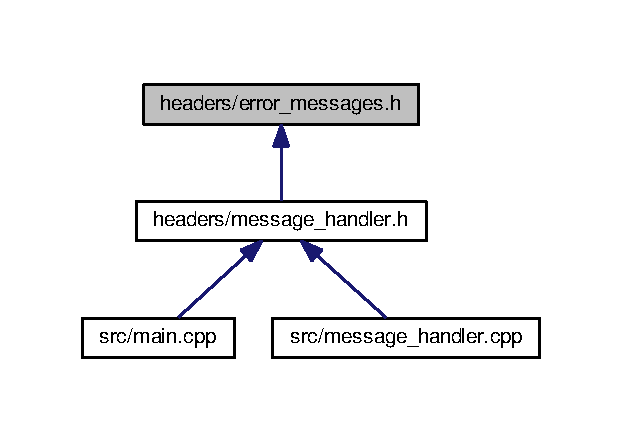
\includegraphics[width=299pt]{error__messages_8h__dep__incl}
\end{center}
\end{figure}
\subsection*{Enumerations}
\begin{DoxyCompactItemize}
\item 
enum \hyperlink{error__messages_8h_af8d1d72c71dcf239d1bf17fe2a760395}{Error\+Message} \{ \\*
\hyperlink{error__messages_8h_af8d1d72c71dcf239d1bf17fe2a760395a5c6be9c004324dc877df6f45fd574cea}{W\+R\+O\+N\+G\+\_\+\+I\+N\+P\+UT}, 
\hyperlink{error__messages_8h_af8d1d72c71dcf239d1bf17fe2a760395a33b1e659fa6fb3a75626cf6888a3ef9f}{C\+A\+N\+T\+\_\+\+O\+P\+E\+N\+\_\+\+A\+C\+C\+\_\+\+V\+I\+D\+EO}, 
\hyperlink{error__messages_8h_af8d1d72c71dcf239d1bf17fe2a760395af629692d52b9e3690257895b6fe2e697}{C\+A\+N\+T\+\_\+\+C\+R\+E\+A\+T\+E\+\_\+\+O\+U\+T\+\_\+\+V\+I\+D\+EO}, 
\hyperlink{error__messages_8h_af8d1d72c71dcf239d1bf17fe2a760395ad4fb339e5527d5a42c9d09446c76b0db}{C\+A\+N\+T\+\_\+\+O\+P\+E\+N\+\_\+\+O\+R\+I\+\_\+\+V\+I\+D\+EO}, 
\\*
\hyperlink{error__messages_8h_af8d1d72c71dcf239d1bf17fe2a760395ad90647fa1d72f0b6c173469d786559ed}{C\+A\+N\+T\+\_\+\+O\+P\+E\+N\+\_\+\+C\+SV}, 
\hyperlink{error__messages_8h_af8d1d72c71dcf239d1bf17fe2a760395a7c06dc9631fd1b5b72c53b99f014e853}{C\+A\+N\+T\+\_\+\+C\+R\+E\+A\+T\+E\+\_\+\+D\+IR}, 
\hyperlink{error__messages_8h_af8d1d72c71dcf239d1bf17fe2a760395a67f3d791eb0d7c3aa28a9aae2cc24deb}{C\+A\+N\+T\+\_\+\+C\+R\+E\+A\+T\+E\+\_\+\+L\+OG}, 
\hyperlink{error__messages_8h_af8d1d72c71dcf239d1bf17fe2a760395aeb11722c84f450400e3b7c4bbeb89ef1}{R\+A\+N\+G\+E\+\_\+\+W\+R\+O\+N\+G\+L\+Y\+\_\+\+D\+E\+F\+I\+N\+ED}, 
\\*
\hyperlink{error__messages_8h_af8d1d72c71dcf239d1bf17fe2a760395a3a1fec2c96b2446726a842e86aa26893}{C\+A\+N\+T\+\_\+\+O\+P\+E\+N\+\_\+\+S\+E\+M\+A\+N\+T\+I\+C\+\_\+\+C\+SV}, 
\hyperlink{error__messages_8h_af8d1d72c71dcf239d1bf17fe2a760395a6d275ef4daeafe84ea9bdfeda944ff8c}{L\+A\+R\+G\+E\+\_\+\+T\+R\+A\+N\+S\+I\+T\+I\+ON}
 \}\begin{DoxyCompactList}\small\item\em The Error\+Message enum The program can {\bfseries exit} with following codes\+: ~\newline
{\bfseries -\/1} -\/ Wrong number of input parameters. \end{DoxyCompactList}
\end{DoxyCompactItemize}


\subsection{Enumeration Type Documentation}
\index{error\+\_\+messages.\+h@{error\+\_\+messages.\+h}!Error\+Message@{Error\+Message}}
\index{Error\+Message@{Error\+Message}!error\+\_\+messages.\+h@{error\+\_\+messages.\+h}}
\subsubsection[{\texorpdfstring{Error\+Message}{ErrorMessage}}]{\setlength{\rightskip}{0pt plus 5cm}enum {\bf Error\+Message}}\hypertarget{error__messages_8h_af8d1d72c71dcf239d1bf17fe2a760395}{}\label{error__messages_8h_af8d1d72c71dcf239d1bf17fe2a760395}


The Error\+Message enum The program can {\bfseries exit} with following codes\+: ~\newline
{\bfseries -\/1} -\/ Wrong number of input parameters. 

~\newline
{\bfseries -\/2} -\/ Experiment id does not exist. ~\newline
{\bfseries -\/3} -\/ Can not open the accelerated video. ~\newline
{\bfseries -\/4} -\/ Can not create file to save the output video. ~\newline
{\bfseries -\/5} -\/ Can not open the video original video. ~\newline
{\bfseries -\/6} -\/ Can not open the C\+SV file with the selected frame numbers of the accelerated video. ~\newline
{\bfseries -\/7} -\/ Can not create directory to save the output data. ~\newline
{\bfseries -\/8} -\/ Can not create log text file. ~\newline
{\bfseries -\/9} -\/ Range limits is not well defined. ~\newline
{\bfseries -\/10} -\/ Can not open the C\+SV file with the semantic costs of the original video. ~\newline
{\bfseries -\/11} -\/ Transition from frame\+\_\+src to frame\+\_\+dst larger than number of transitions described in the file of the semantic costs $\ast$ \begin{Desc}
\item[Enumerator]\par
\begin{description}
\index{W\+R\+O\+N\+G\+\_\+\+I\+N\+P\+UT@{W\+R\+O\+N\+G\+\_\+\+I\+N\+P\+UT}!error\+\_\+messages.\+h@{error\+\_\+messages.\+h}}\index{error\+\_\+messages.\+h@{error\+\_\+messages.\+h}!W\+R\+O\+N\+G\+\_\+\+I\+N\+P\+UT@{W\+R\+O\+N\+G\+\_\+\+I\+N\+P\+UT}}\item[{\em 
W\+R\+O\+N\+G\+\_\+\+I\+N\+P\+UT\hypertarget{error__messages_8h_af8d1d72c71dcf239d1bf17fe2a760395a5c6be9c004324dc877df6f45fd574cea}{}\label{error__messages_8h_af8d1d72c71dcf239d1bf17fe2a760395a5c6be9c004324dc877df6f45fd574cea}
}]\index{C\+A\+N\+T\+\_\+\+O\+P\+E\+N\+\_\+\+A\+C\+C\+\_\+\+V\+I\+D\+EO@{C\+A\+N\+T\+\_\+\+O\+P\+E\+N\+\_\+\+A\+C\+C\+\_\+\+V\+I\+D\+EO}!error\+\_\+messages.\+h@{error\+\_\+messages.\+h}}\index{error\+\_\+messages.\+h@{error\+\_\+messages.\+h}!C\+A\+N\+T\+\_\+\+O\+P\+E\+N\+\_\+\+A\+C\+C\+\_\+\+V\+I\+D\+EO@{C\+A\+N\+T\+\_\+\+O\+P\+E\+N\+\_\+\+A\+C\+C\+\_\+\+V\+I\+D\+EO}}\item[{\em 
C\+A\+N\+T\+\_\+\+O\+P\+E\+N\+\_\+\+A\+C\+C\+\_\+\+V\+I\+D\+EO\hypertarget{error__messages_8h_af8d1d72c71dcf239d1bf17fe2a760395a33b1e659fa6fb3a75626cf6888a3ef9f}{}\label{error__messages_8h_af8d1d72c71dcf239d1bf17fe2a760395a33b1e659fa6fb3a75626cf6888a3ef9f}
}]\index{C\+A\+N\+T\+\_\+\+C\+R\+E\+A\+T\+E\+\_\+\+O\+U\+T\+\_\+\+V\+I\+D\+EO@{C\+A\+N\+T\+\_\+\+C\+R\+E\+A\+T\+E\+\_\+\+O\+U\+T\+\_\+\+V\+I\+D\+EO}!error\+\_\+messages.\+h@{error\+\_\+messages.\+h}}\index{error\+\_\+messages.\+h@{error\+\_\+messages.\+h}!C\+A\+N\+T\+\_\+\+C\+R\+E\+A\+T\+E\+\_\+\+O\+U\+T\+\_\+\+V\+I\+D\+EO@{C\+A\+N\+T\+\_\+\+C\+R\+E\+A\+T\+E\+\_\+\+O\+U\+T\+\_\+\+V\+I\+D\+EO}}\item[{\em 
C\+A\+N\+T\+\_\+\+C\+R\+E\+A\+T\+E\+\_\+\+O\+U\+T\+\_\+\+V\+I\+D\+EO\hypertarget{error__messages_8h_af8d1d72c71dcf239d1bf17fe2a760395af629692d52b9e3690257895b6fe2e697}{}\label{error__messages_8h_af8d1d72c71dcf239d1bf17fe2a760395af629692d52b9e3690257895b6fe2e697}
}]\index{C\+A\+N\+T\+\_\+\+O\+P\+E\+N\+\_\+\+O\+R\+I\+\_\+\+V\+I\+D\+EO@{C\+A\+N\+T\+\_\+\+O\+P\+E\+N\+\_\+\+O\+R\+I\+\_\+\+V\+I\+D\+EO}!error\+\_\+messages.\+h@{error\+\_\+messages.\+h}}\index{error\+\_\+messages.\+h@{error\+\_\+messages.\+h}!C\+A\+N\+T\+\_\+\+O\+P\+E\+N\+\_\+\+O\+R\+I\+\_\+\+V\+I\+D\+EO@{C\+A\+N\+T\+\_\+\+O\+P\+E\+N\+\_\+\+O\+R\+I\+\_\+\+V\+I\+D\+EO}}\item[{\em 
C\+A\+N\+T\+\_\+\+O\+P\+E\+N\+\_\+\+O\+R\+I\+\_\+\+V\+I\+D\+EO\hypertarget{error__messages_8h_af8d1d72c71dcf239d1bf17fe2a760395ad4fb339e5527d5a42c9d09446c76b0db}{}\label{error__messages_8h_af8d1d72c71dcf239d1bf17fe2a760395ad4fb339e5527d5a42c9d09446c76b0db}
}]\index{C\+A\+N\+T\+\_\+\+O\+P\+E\+N\+\_\+\+C\+SV@{C\+A\+N\+T\+\_\+\+O\+P\+E\+N\+\_\+\+C\+SV}!error\+\_\+messages.\+h@{error\+\_\+messages.\+h}}\index{error\+\_\+messages.\+h@{error\+\_\+messages.\+h}!C\+A\+N\+T\+\_\+\+O\+P\+E\+N\+\_\+\+C\+SV@{C\+A\+N\+T\+\_\+\+O\+P\+E\+N\+\_\+\+C\+SV}}\item[{\em 
C\+A\+N\+T\+\_\+\+O\+P\+E\+N\+\_\+\+C\+SV\hypertarget{error__messages_8h_af8d1d72c71dcf239d1bf17fe2a760395ad90647fa1d72f0b6c173469d786559ed}{}\label{error__messages_8h_af8d1d72c71dcf239d1bf17fe2a760395ad90647fa1d72f0b6c173469d786559ed}
}]\index{C\+A\+N\+T\+\_\+\+C\+R\+E\+A\+T\+E\+\_\+\+D\+IR@{C\+A\+N\+T\+\_\+\+C\+R\+E\+A\+T\+E\+\_\+\+D\+IR}!error\+\_\+messages.\+h@{error\+\_\+messages.\+h}}\index{error\+\_\+messages.\+h@{error\+\_\+messages.\+h}!C\+A\+N\+T\+\_\+\+C\+R\+E\+A\+T\+E\+\_\+\+D\+IR@{C\+A\+N\+T\+\_\+\+C\+R\+E\+A\+T\+E\+\_\+\+D\+IR}}\item[{\em 
C\+A\+N\+T\+\_\+\+C\+R\+E\+A\+T\+E\+\_\+\+D\+IR\hypertarget{error__messages_8h_af8d1d72c71dcf239d1bf17fe2a760395a7c06dc9631fd1b5b72c53b99f014e853}{}\label{error__messages_8h_af8d1d72c71dcf239d1bf17fe2a760395a7c06dc9631fd1b5b72c53b99f014e853}
}]\index{C\+A\+N\+T\+\_\+\+C\+R\+E\+A\+T\+E\+\_\+\+L\+OG@{C\+A\+N\+T\+\_\+\+C\+R\+E\+A\+T\+E\+\_\+\+L\+OG}!error\+\_\+messages.\+h@{error\+\_\+messages.\+h}}\index{error\+\_\+messages.\+h@{error\+\_\+messages.\+h}!C\+A\+N\+T\+\_\+\+C\+R\+E\+A\+T\+E\+\_\+\+L\+OG@{C\+A\+N\+T\+\_\+\+C\+R\+E\+A\+T\+E\+\_\+\+L\+OG}}\item[{\em 
C\+A\+N\+T\+\_\+\+C\+R\+E\+A\+T\+E\+\_\+\+L\+OG\hypertarget{error__messages_8h_af8d1d72c71dcf239d1bf17fe2a760395a67f3d791eb0d7c3aa28a9aae2cc24deb}{}\label{error__messages_8h_af8d1d72c71dcf239d1bf17fe2a760395a67f3d791eb0d7c3aa28a9aae2cc24deb}
}]\index{R\+A\+N\+G\+E\+\_\+\+W\+R\+O\+N\+G\+L\+Y\+\_\+\+D\+E\+F\+I\+N\+ED@{R\+A\+N\+G\+E\+\_\+\+W\+R\+O\+N\+G\+L\+Y\+\_\+\+D\+E\+F\+I\+N\+ED}!error\+\_\+messages.\+h@{error\+\_\+messages.\+h}}\index{error\+\_\+messages.\+h@{error\+\_\+messages.\+h}!R\+A\+N\+G\+E\+\_\+\+W\+R\+O\+N\+G\+L\+Y\+\_\+\+D\+E\+F\+I\+N\+ED@{R\+A\+N\+G\+E\+\_\+\+W\+R\+O\+N\+G\+L\+Y\+\_\+\+D\+E\+F\+I\+N\+ED}}\item[{\em 
R\+A\+N\+G\+E\+\_\+\+W\+R\+O\+N\+G\+L\+Y\+\_\+\+D\+E\+F\+I\+N\+ED\hypertarget{error__messages_8h_af8d1d72c71dcf239d1bf17fe2a760395aeb11722c84f450400e3b7c4bbeb89ef1}{}\label{error__messages_8h_af8d1d72c71dcf239d1bf17fe2a760395aeb11722c84f450400e3b7c4bbeb89ef1}
}]\index{C\+A\+N\+T\+\_\+\+O\+P\+E\+N\+\_\+\+S\+E\+M\+A\+N\+T\+I\+C\+\_\+\+C\+SV@{C\+A\+N\+T\+\_\+\+O\+P\+E\+N\+\_\+\+S\+E\+M\+A\+N\+T\+I\+C\+\_\+\+C\+SV}!error\+\_\+messages.\+h@{error\+\_\+messages.\+h}}\index{error\+\_\+messages.\+h@{error\+\_\+messages.\+h}!C\+A\+N\+T\+\_\+\+O\+P\+E\+N\+\_\+\+S\+E\+M\+A\+N\+T\+I\+C\+\_\+\+C\+SV@{C\+A\+N\+T\+\_\+\+O\+P\+E\+N\+\_\+\+S\+E\+M\+A\+N\+T\+I\+C\+\_\+\+C\+SV}}\item[{\em 
C\+A\+N\+T\+\_\+\+O\+P\+E\+N\+\_\+\+S\+E\+M\+A\+N\+T\+I\+C\+\_\+\+C\+SV\hypertarget{error__messages_8h_af8d1d72c71dcf239d1bf17fe2a760395a3a1fec2c96b2446726a842e86aa26893}{}\label{error__messages_8h_af8d1d72c71dcf239d1bf17fe2a760395a3a1fec2c96b2446726a842e86aa26893}
}]\index{L\+A\+R\+G\+E\+\_\+\+T\+R\+A\+N\+S\+I\+T\+I\+ON@{L\+A\+R\+G\+E\+\_\+\+T\+R\+A\+N\+S\+I\+T\+I\+ON}!error\+\_\+messages.\+h@{error\+\_\+messages.\+h}}\index{error\+\_\+messages.\+h@{error\+\_\+messages.\+h}!L\+A\+R\+G\+E\+\_\+\+T\+R\+A\+N\+S\+I\+T\+I\+ON@{L\+A\+R\+G\+E\+\_\+\+T\+R\+A\+N\+S\+I\+T\+I\+ON}}\item[{\em 
L\+A\+R\+G\+E\+\_\+\+T\+R\+A\+N\+S\+I\+T\+I\+ON\hypertarget{error__messages_8h_af8d1d72c71dcf239d1bf17fe2a760395a6d275ef4daeafe84ea9bdfeda944ff8c}{}\label{error__messages_8h_af8d1d72c71dcf239d1bf17fe2a760395a6d275ef4daeafe84ea9bdfeda944ff8c}
}]\end{description}
\end{Desc}

\hypertarget{file__operations_8h}{}\section{headers/file\+\_\+operations.h File Reference}
\label{file__operations_8h}\index{headers/file\+\_\+operations.\+h@{headers/file\+\_\+operations.\+h}}


Header functions for the \hyperlink{file__operations_8cpp}{file\+\_\+operations.\+cpp}.  


{\ttfamily \#include $<$stdio.\+h$>$}\\*
{\ttfamily \#include $<$iostream$>$}\\*
{\ttfamily \#include $<$fstream$>$}\\*
{\ttfamily \#include $<$vector$>$}\\*
{\ttfamily \#include $<$cstdlib$>$}\\*
{\ttfamily \#include $<$string$>$}\\*
{\ttfamily \#include $<$algorithm$>$}\\*
{\ttfamily \#include $<$iterator$>$}\\*
{\ttfamily \#include $<$sstream$>$}\\*
{\ttfamily \#include $<$iomanip$>$}\\*
{\ttfamily \#include $<$limits$>$}\\*
{\ttfamily \#include $<$boost/tokenizer.\+hpp$>$}\\*
{\ttfamily \#include $<$boost/algorithm/string.\+hpp$>$}\\*
{\ttfamily \#include \char`\"{}definitions/experiment\+\_\+struct.\+h\char`\"{}}\\*
Include dependency graph for file\+\_\+operations.\+h\+:\nopagebreak
\begin{figure}[H]
\begin{center}
\leavevmode
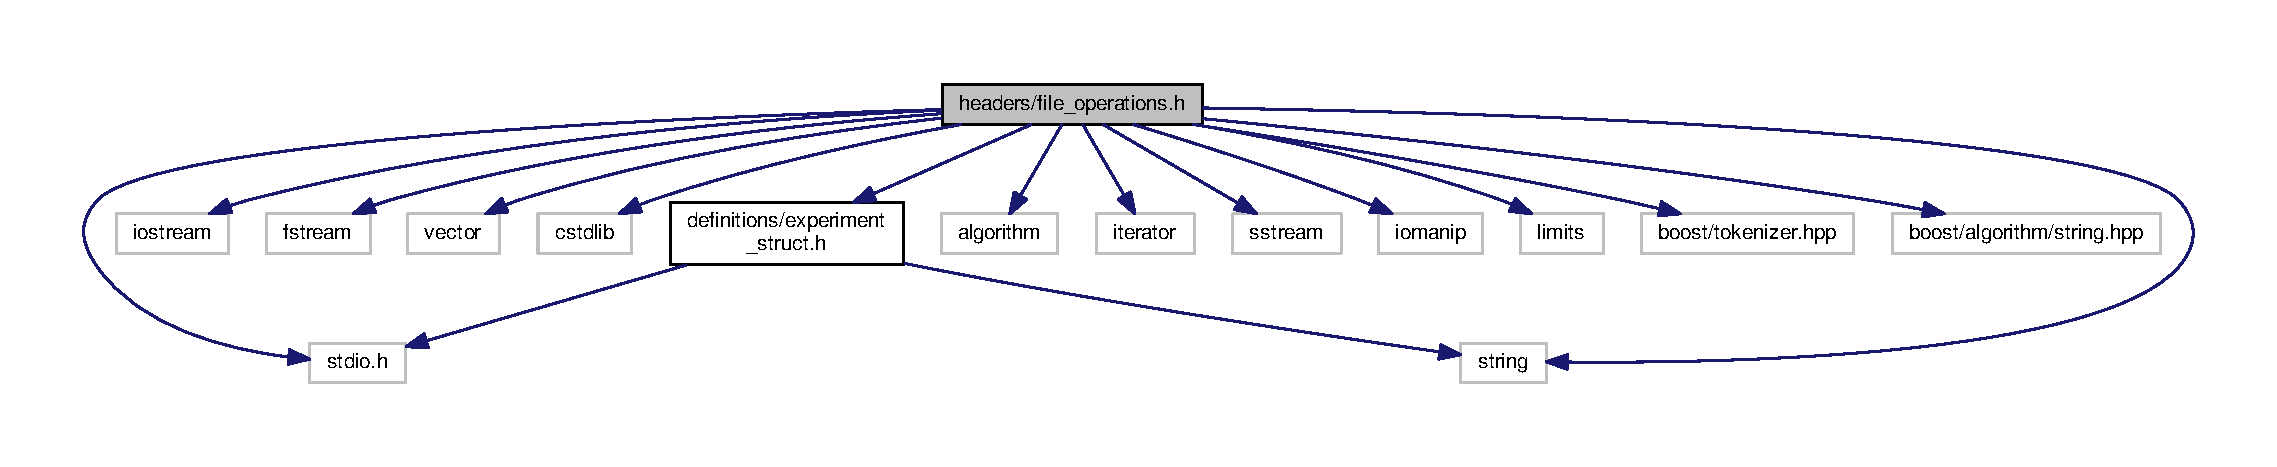
\includegraphics[width=350pt]{file__operations_8h__incl}
\end{center}
\end{figure}
This graph shows which files directly or indirectly include this file\+:\nopagebreak
\begin{figure}[H]
\begin{center}
\leavevmode
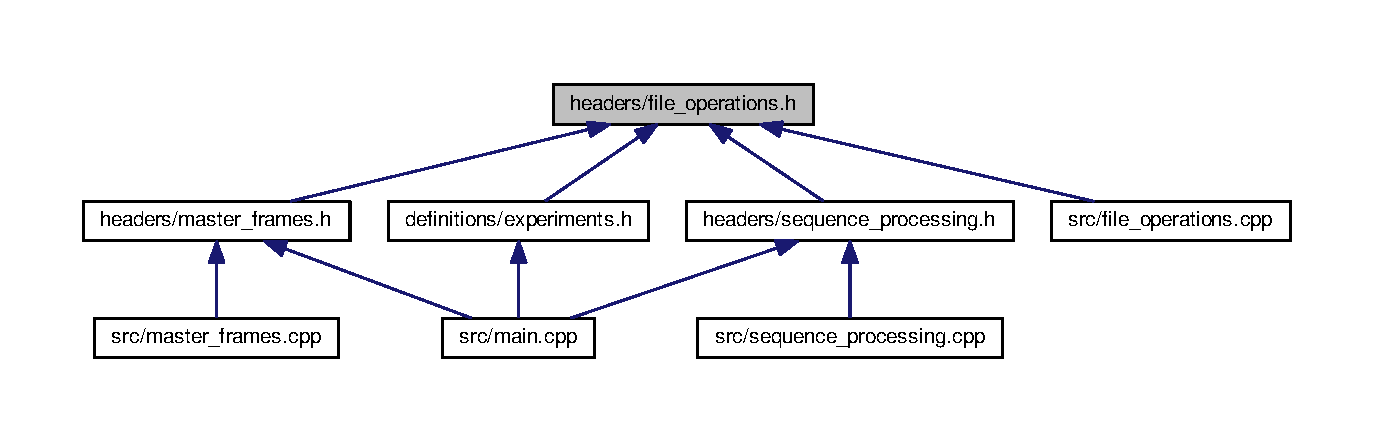
\includegraphics[width=350pt]{file__operations_8h__dep__incl}
\end{center}
\end{figure}
\subsection*{Functions}
\begin{DoxyCompactItemize}
\item 
std\+::vector$<$ int $>$ \hyperlink{file__operations_8h_ad65b52efdd81718726a7c020b2745231}{load\+Master\+Frames\+From\+File} (const \hyperlink{structEXPERIMENT}{E\+X\+P\+E\+R\+I\+M\+E\+NT} \&\hyperlink{main_8cpp_a9f5a81402e170475690f371d55cbe623}{experiment\+\_\+settings})
\begin{DoxyCompactList}\small\item\em Function to load the master frames from a file defined in the field read\+\_\+masterframes\+\_\+filename in the experiment\+\_\+settings. \end{DoxyCompactList}\item 
bool \hyperlink{file__operations_8h_a8ee838aca4ec1d86b6da27d8d0c6c5a6}{save\+Master\+Frames\+To\+File} (const \hyperlink{structEXPERIMENT}{E\+X\+P\+E\+R\+I\+M\+E\+NT} \&\hyperlink{main_8cpp_a9f5a81402e170475690f371d55cbe623}{experiment\+\_\+settings}, const std\+::vector$<$ int $>$ masters\+\_\+frames)
\begin{DoxyCompactList}\small\item\em Function to save the calculated master frames into a file defined in the field save\+\_\+masterframes\+\_\+filename in the experiment\+\_\+settings. \end{DoxyCompactList}\item 
void \hyperlink{file__operations_8h_a65c5cb4d2def7f9475ee950799649709}{read\+Selected\+Frames\+C\+SV} (std\+::string filename, std\+::vector$<$ int $>$ \&selected\+\_\+frames)
\begin{DoxyCompactList}\small\item\em Function to read a C\+SV composed by frames selected by the selection algorithm. \end{DoxyCompactList}\item 
std\+::string \hyperlink{file__operations_8h_add54304682603740491ac7f2fa3e8909}{get\+Experiment\+Id} ()
\begin{DoxyCompactList}\small\item\em Function that manages the experiments ID automatically. \end{DoxyCompactList}\item 
double \hyperlink{file__operations_8h_a4389609d14f1f46754e68ced749e4736}{get\+Semantic\+Cost} (const \hyperlink{structEXPERIMENT}{E\+X\+P\+E\+R\+I\+M\+E\+NT} \&\hyperlink{main_8cpp_a9f5a81402e170475690f371d55cbe623}{experiment\+\_\+settings}, const int frame\+\_\+src, const int frame\+\_\+dst)
\begin{DoxyCompactList}\small\item\em Function that returns the semantic cost of the transiction from the frame\+\_\+src to the frame\+\_\+dst. \end{DoxyCompactList}\item 
std\+::vector$<$ std\+::vector$<$ double $>$ $>$ \hyperlink{file__operations_8h_a2995a8f3930a0b01a4e0ac1bfc5638e3}{load\+Instability\+Costs\+From\+File} (const \hyperlink{structEXPERIMENT}{E\+X\+P\+E\+R\+I\+M\+E\+NT} \&\hyperlink{main_8cpp_a9f5a81402e170475690f371d55cbe623}{experiment\+\_\+settings})
\begin{DoxyCompactList}\small\item\em load\+Instability\+Costs\+From\+File Loads the instability costs from a C\+SV file (matrix format). \end{DoxyCompactList}\item 
std\+::vector$<$ std\+::vector$<$ double $>$ $>$ \hyperlink{file__operations_8h_af95138c7e9d6611e1ace10ec85b633eb}{load\+Optical\+Flow} (const \hyperlink{structEXPERIMENT}{E\+X\+P\+E\+R\+I\+M\+E\+NT} \&\hyperlink{main_8cpp_a9f5a81402e170475690f371d55cbe623}{experiment\+\_\+settings})
\begin{DoxyCompactList}\small\item\em load\+Optical\+Flow Loads the Optical Flow calculated by the Flow\+Net from a C\+SV file. \end{DoxyCompactList}\item 
bool \hyperlink{file__operations_8h_a1e52e743807e450c3bdc8d8a179093ce}{str2bool} (std\+::string str)
\begin{DoxyCompactList}\small\item\em str2bool convert a string to boolean. \end{DoxyCompactList}\item 
std\+::string \hyperlink{file__operations_8h_a6fee1fe59a7b7ffbfff04e8e9b9e6571}{filter\+\_\+string} (std\+::string str)
\begin{DoxyCompactList}\small\item\em filter\+\_\+string filter a string to remove white spaces and line break. \end{DoxyCompactList}\end{DoxyCompactItemize}


\subsection{Detailed Description}
Header functions for the \hyperlink{file__operations_8cpp}{file\+\_\+operations.\+cpp}. 



\subsection{Function Documentation}
\index{file\+\_\+operations.\+h@{file\+\_\+operations.\+h}!filter\+\_\+string@{filter\+\_\+string}}
\index{filter\+\_\+string@{filter\+\_\+string}!file\+\_\+operations.\+h@{file\+\_\+operations.\+h}}
\subsubsection[{\texorpdfstring{filter\+\_\+string(std\+::string str)}{filter\_string(std::string str)}}]{\setlength{\rightskip}{0pt plus 5cm}std\+::string filter\+\_\+string (
\begin{DoxyParamCaption}
\item[{std\+::string}]{str}
\end{DoxyParamCaption}
)}\hypertarget{file__operations_8h_a6fee1fe59a7b7ffbfff04e8e9b9e6571}{}\label{file__operations_8h_a6fee1fe59a7b7ffbfff04e8e9b9e6571}


filter\+\_\+string filter a string to remove white spaces and line break. 


\begin{DoxyParams}{Parameters}
{\em str} & -\/ string to be filtered \\
\hline
\end{DoxyParams}
\begin{DoxyReturn}{Returns}
str -\/ filtered string
\end{DoxyReturn}
\begin{DoxyAuthor}{Author}
Felipe Cadar Chamone 
\end{DoxyAuthor}
\begin{DoxyDate}{Date}
14/07/2017
\end{DoxyDate}

\begin{DoxyParams}{Parameters}
{\em string} & \\
\hline
\end{DoxyParams}
\begin{DoxyReturn}{Returns}
string
\end{DoxyReturn}
\begin{DoxyAuthor}{Author}
Felipe Cadar Chamone 
\end{DoxyAuthor}
\begin{DoxyDate}{Date}
14/07/2017 
\end{DoxyDate}
\index{file\+\_\+operations.\+h@{file\+\_\+operations.\+h}!get\+Experiment\+Id@{get\+Experiment\+Id}}
\index{get\+Experiment\+Id@{get\+Experiment\+Id}!file\+\_\+operations.\+h@{file\+\_\+operations.\+h}}
\subsubsection[{\texorpdfstring{get\+Experiment\+Id()}{getExperimentId()}}]{\setlength{\rightskip}{0pt plus 5cm}std\+::string get\+Experiment\+Id (
\begin{DoxyParamCaption}
{}
\end{DoxyParamCaption}
)}\hypertarget{file__operations_8h_add54304682603740491ac7f2fa3e8909}{}\label{file__operations_8h_add54304682603740491ac7f2fa3e8909}


Function that manages the experiments ID automatically. 

\begin{DoxyReturn}{Returns}
{\ttfamily std\+::string} -\/ The experiment id formatted by 4 digits
\end{DoxyReturn}
\begin{DoxyAuthor}{Author}
Washington Luis de Souza Ramos 
\end{DoxyAuthor}
\begin{DoxyDate}{Date}
19/04/2016 
\end{DoxyDate}
\index{file\+\_\+operations.\+h@{file\+\_\+operations.\+h}!get\+Semantic\+Cost@{get\+Semantic\+Cost}}
\index{get\+Semantic\+Cost@{get\+Semantic\+Cost}!file\+\_\+operations.\+h@{file\+\_\+operations.\+h}}
\subsubsection[{\texorpdfstring{get\+Semantic\+Cost(const E\+X\+P\+E\+R\+I\+M\+E\+N\+T \&experiment\+\_\+settings, const int frame\+\_\+src, const int frame\+\_\+dst)}{getSemanticCost(const EXPERIMENT \&experiment\_settings, const int frame\_src, const int frame\_dst)}}]{\setlength{\rightskip}{0pt plus 5cm}double get\+Semantic\+Cost (
\begin{DoxyParamCaption}
\item[{const {\bf E\+X\+P\+E\+R\+I\+M\+E\+NT} \&}]{experiment\+\_\+settings, }
\item[{const int}]{frame\+\_\+src, }
\item[{const int}]{frame\+\_\+dst}
\end{DoxyParamCaption}
)}\hypertarget{file__operations_8h_a4389609d14f1f46754e68ced749e4736}{}\label{file__operations_8h_a4389609d14f1f46754e68ced749e4736}


Function that returns the semantic cost of the transiction from the frame\+\_\+src to the frame\+\_\+dst. 

The file where the semantic cost will be find is defined in the experiment\+\_\+settings


\begin{DoxyParams}{Parameters}
{\em experiment\+\_\+settings} & -\/ variable with the experiment setting. \\
\hline
{\em frame\+\_\+src} & -\/ first frame of the transition. \\
\hline
{\em frame\+\_\+dst} & -\/ last frame of the transition.\\
\hline
\end{DoxyParams}
\begin{DoxyReturn}{Returns}
{\ttfamily double} -\/ The semantic cost of the transiction of the frame\+\_\+src to the frame\+\_\+dst. Returns the complementary value ( 1 -\/ x ).
\end{DoxyReturn}
\begin{DoxyAuthor}{Author}
Michel Melo da Silva 
\end{DoxyAuthor}
\begin{DoxyDate}{Date}
30/04/2016
\end{DoxyDate}
Function that returns the semantic cost of the transiction from the frame\+\_\+src to the frame\+\_\+dst.

The file where the semantic cost will be find is defined in the experiment\+\_\+settings


\begin{DoxyParams}{Parameters}
{\em experiment\+\_\+settings} & -\/ variable with the experiment setting. \\
\hline
{\em frame\+\_\+src} & -\/ first frame of the transition. \\
\hline
{\em frame\+\_\+dst} & -\/ last frame of the transition.\\
\hline
\end{DoxyParams}
\begin{DoxyReturn}{Returns}
{\ttfamily double} -\/ The semantic cost of the transiction of the frame\+\_\+src to the frame\+\_\+dst. Returns the complementary value ( 1 -\/ x ).
\end{DoxyReturn}
\begin{DoxyAuthor}{Author}
Michel Melo da Silva 
\end{DoxyAuthor}
\begin{DoxyDate}{Date}
30/04/2016 
\end{DoxyDate}
\index{file\+\_\+operations.\+h@{file\+\_\+operations.\+h}!load\+Instability\+Costs\+From\+File@{load\+Instability\+Costs\+From\+File}}
\index{load\+Instability\+Costs\+From\+File@{load\+Instability\+Costs\+From\+File}!file\+\_\+operations.\+h@{file\+\_\+operations.\+h}}
\subsubsection[{\texorpdfstring{load\+Instability\+Costs\+From\+File(const E\+X\+P\+E\+R\+I\+M\+E\+N\+T \&experiment\+\_\+settings)}{loadInstabilityCostsFromFile(const EXPERIMENT \&experiment\_settings)}}]{\setlength{\rightskip}{0pt plus 5cm}std\+::vector$<$ std\+::vector$<$double$>$ $>$ load\+Instability\+Costs\+From\+File (
\begin{DoxyParamCaption}
\item[{const {\bf E\+X\+P\+E\+R\+I\+M\+E\+NT} \&}]{experiment\+\_\+settings}
\end{DoxyParamCaption}
)}\hypertarget{file__operations_8h_a2995a8f3930a0b01a4e0ac1bfc5638e3}{}\label{file__operations_8h_a2995a8f3930a0b01a4e0ac1bfc5638e3}


load\+Instability\+Costs\+From\+File Loads the instability costs from a C\+SV file (matrix format). 


\begin{DoxyParams}{Parameters}
{\em experiment\+\_\+settings} & \\
\hline
\end{DoxyParams}
\begin{DoxyReturn}{Returns}
The matrix of instability costs
\end{DoxyReturn}
\begin{DoxyAuthor}{Author}
Washington Luis de Souza Ramos 
\end{DoxyAuthor}
\begin{DoxyDate}{Date}
12/09/2016 
\end{DoxyDate}
\index{file\+\_\+operations.\+h@{file\+\_\+operations.\+h}!load\+Master\+Frames\+From\+File@{load\+Master\+Frames\+From\+File}}
\index{load\+Master\+Frames\+From\+File@{load\+Master\+Frames\+From\+File}!file\+\_\+operations.\+h@{file\+\_\+operations.\+h}}
\subsubsection[{\texorpdfstring{load\+Master\+Frames\+From\+File(const E\+X\+P\+E\+R\+I\+M\+E\+N\+T \&experiment\+\_\+settings)}{loadMasterFramesFromFile(const EXPERIMENT \&experiment\_settings)}}]{\setlength{\rightskip}{0pt plus 5cm}std\+::vector$<$int$>$ load\+Master\+Frames\+From\+File (
\begin{DoxyParamCaption}
\item[{const {\bf E\+X\+P\+E\+R\+I\+M\+E\+NT} \&}]{experiment\+\_\+settings}
\end{DoxyParamCaption}
)}\hypertarget{file__operations_8h_ad65b52efdd81718726a7c020b2745231}{}\label{file__operations_8h_ad65b52efdd81718726a7c020b2745231}


Function to load the master frames from a file defined in the field read\+\_\+masterframes\+\_\+filename in the experiment\+\_\+settings. 


\begin{DoxyParams}{Parameters}
{\em experiment\+\_\+settings} & -\/ variable with the experiment setting.\\
\hline
\end{DoxyParams}
\begin{DoxyReturn}{Returns}
{\ttfamily std\+::vector} -\/ vector of master frames loaded from file describle in the experiment settings.
\end{DoxyReturn}
\begin{DoxyAuthor}{Author}
Michel Melo da Silva 
\end{DoxyAuthor}
\begin{DoxyDate}{Date}
08/04/2016 
\end{DoxyDate}
\index{file\+\_\+operations.\+h@{file\+\_\+operations.\+h}!load\+Optical\+Flow@{load\+Optical\+Flow}}
\index{load\+Optical\+Flow@{load\+Optical\+Flow}!file\+\_\+operations.\+h@{file\+\_\+operations.\+h}}
\subsubsection[{\texorpdfstring{load\+Optical\+Flow(const E\+X\+P\+E\+R\+I\+M\+E\+N\+T \&experiment\+\_\+settings)}{loadOpticalFlow(const EXPERIMENT \&experiment\_settings)}}]{\setlength{\rightskip}{0pt plus 5cm}std\+::vector$<$ std\+::vector$<$double$>$ $>$ load\+Optical\+Flow (
\begin{DoxyParamCaption}
\item[{const {\bf E\+X\+P\+E\+R\+I\+M\+E\+NT} \&}]{experiment\+\_\+settings}
\end{DoxyParamCaption}
)}\hypertarget{file__operations_8h_af95138c7e9d6611e1ace10ec85b633eb}{}\label{file__operations_8h_af95138c7e9d6611e1ace10ec85b633eb}


load\+Optical\+Flow Loads the Optical Flow calculated by the Flow\+Net from a C\+SV file. 


\begin{DoxyParams}{Parameters}
{\em experiment\+\_\+settings} & \\
\hline
\end{DoxyParams}
\begin{DoxyReturn}{Returns}
Vector\mbox{[}j\mbox{]}\mbox{[}i\mbox{]} with the optical flow from the image j to j+1 (i=0 is dx and i=1 is dy).
\end{DoxyReturn}
\begin{DoxyAuthor}{Author}
Michel Melo da Silva 
\end{DoxyAuthor}
\begin{DoxyDate}{Date}
09/01/2017 
\end{DoxyDate}
\index{file\+\_\+operations.\+h@{file\+\_\+operations.\+h}!read\+Selected\+Frames\+C\+SV@{read\+Selected\+Frames\+C\+SV}}
\index{read\+Selected\+Frames\+C\+SV@{read\+Selected\+Frames\+C\+SV}!file\+\_\+operations.\+h@{file\+\_\+operations.\+h}}
\subsubsection[{\texorpdfstring{read\+Selected\+Frames\+C\+S\+V(std\+::string filename, std\+::vector$<$ int $>$ \&selected\+\_\+frames)}{readSelectedFramesCSV(std::string filename, std::vector< int > \&selected\_frames)}}]{\setlength{\rightskip}{0pt plus 5cm}void read\+Selected\+Frames\+C\+SV (
\begin{DoxyParamCaption}
\item[{std\+::string}]{filename, }
\item[{std\+::vector$<$ int $>$ \&}]{selected\+\_\+frames}
\end{DoxyParamCaption}
)}\hypertarget{file__operations_8h_a65c5cb4d2def7f9475ee950799649709}{}\label{file__operations_8h_a65c5cb4d2def7f9475ee950799649709}


Function to read a C\+SV composed by frames selected by the selection algorithm. 


\begin{DoxyParams}{Parameters}
{\em filename} & -\/ std\+::string with the filename of the C\+SV file that contains the selected frames of the reduced video. \\
\hline
{\em selected\+\_\+frames} & -\/ vector to save the selected frames.\\
\hline
\end{DoxyParams}
\begin{DoxyReturn}{Returns}
{\ttfamily void} 
\end{DoxyReturn}
\begin{DoxyAuthor}{Author}
Washington Luis de Souza Ramos 
\end{DoxyAuthor}
\begin{DoxyDate}{Date}
14/04/2016 
\end{DoxyDate}
\index{file\+\_\+operations.\+h@{file\+\_\+operations.\+h}!save\+Master\+Frames\+To\+File@{save\+Master\+Frames\+To\+File}}
\index{save\+Master\+Frames\+To\+File@{save\+Master\+Frames\+To\+File}!file\+\_\+operations.\+h@{file\+\_\+operations.\+h}}
\subsubsection[{\texorpdfstring{save\+Master\+Frames\+To\+File(const E\+X\+P\+E\+R\+I\+M\+E\+N\+T \&experiment\+\_\+settings, const std\+::vector$<$ int $>$ masters\+\_\+frames)}{saveMasterFramesToFile(const EXPERIMENT \&experiment\_settings, const std::vector< int > masters\_frames)}}]{\setlength{\rightskip}{0pt plus 5cm}bool save\+Master\+Frames\+To\+File (
\begin{DoxyParamCaption}
\item[{const {\bf E\+X\+P\+E\+R\+I\+M\+E\+NT} \&}]{experiment\+\_\+settings, }
\item[{const std\+::vector$<$ int $>$}]{masters\+\_\+frames}
\end{DoxyParamCaption}
)}\hypertarget{file__operations_8h_a8ee838aca4ec1d86b6da27d8d0c6c5a6}{}\label{file__operations_8h_a8ee838aca4ec1d86b6da27d8d0c6c5a6}


Function to save the calculated master frames into a file defined in the field save\+\_\+masterframes\+\_\+filename in the experiment\+\_\+settings. 


\begin{DoxyParams}{Parameters}
{\em experiment\+\_\+settings} & -\/ variable with the experiment setting. \\
\hline
{\em masters\+\_\+frames} & -\/ vector of master frames to be saved in file describle in the experiment settings.\\
\hline
\end{DoxyParams}
\begin{DoxyReturn}{Returns}
{\ttfamily bool} {\bfseries true} -\/ if the writer return sucess while writing the file. ~\newline
 {\ttfamily bool} {\bfseries false} -\/ if the writer return fail while writing the file.
\end{DoxyReturn}
\begin{DoxyAuthor}{Author}
Michel Melo da Silva 
\end{DoxyAuthor}
\begin{DoxyDate}{Date}
08/04/2016 
\end{DoxyDate}
\index{file\+\_\+operations.\+h@{file\+\_\+operations.\+h}!str2bool@{str2bool}}
\index{str2bool@{str2bool}!file\+\_\+operations.\+h@{file\+\_\+operations.\+h}}
\subsubsection[{\texorpdfstring{str2bool(std\+::string str)}{str2bool(std::string str)}}]{\setlength{\rightskip}{0pt plus 5cm}bool str2bool (
\begin{DoxyParamCaption}
\item[{std\+::string}]{str}
\end{DoxyParamCaption}
)}\hypertarget{file__operations_8h_a1e52e743807e450c3bdc8d8a179093ce}{}\label{file__operations_8h_a1e52e743807e450c3bdc8d8a179093ce}


str2bool convert a string to boolean. 


\begin{DoxyParams}{Parameters}
{\em str} & -\/ string to convert \\
\hline
\end{DoxyParams}
\begin{DoxyReturn}{Returns}
boolean
\end{DoxyReturn}
\begin{DoxyAuthor}{Author}
Felipe Cadar Chamone 
\end{DoxyAuthor}
\begin{DoxyDate}{Date}
14/07/2017
\end{DoxyDate}

\begin{DoxyParams}{Parameters}
{\em string} & \\
\hline
\end{DoxyParams}
\begin{DoxyReturn}{Returns}
boolean
\end{DoxyReturn}
\begin{DoxyAuthor}{Author}
Felipe Cadar Chamone 
\end{DoxyAuthor}
\begin{DoxyDate}{Date}
14/07/2017 
\end{DoxyDate}

\hypertarget{homography_8h}{}\section{headers/homography.h File Reference}
\label{homography_8h}\index{headers/homography.\+h@{headers/homography.\+h}}


Header functions for the \hyperlink{homography_8cpp}{homography.\+cpp}.  


{\ttfamily \#include $<$stdio.\+h$>$}\\*
{\ttfamily \#include $<$iostream$>$}\\*
{\ttfamily \#include $<$opencv2/core/core.\+hpp$>$}\\*
{\ttfamily \#include $<$opencv2/features2d/features2d.\+hpp$>$}\\*
{\ttfamily \#include $<$opencv2/highgui/highgui.\+hpp$>$}\\*
{\ttfamily \#include $<$opencv2/nonfree/nonfree.\+hpp$>$}\\*
{\ttfamily \#include $<$opencv2/calib3d/calib3d.\+hpp$>$}\\*
{\ttfamily \#include $<$opencv2/imgproc/imgproc.\+hpp$>$}\\*
{\ttfamily \#include \char`\"{}definitions/define.\+h\char`\"{}}\\*
Include dependency graph for homography.\+h\+:\nopagebreak
\begin{figure}[H]
\begin{center}
\leavevmode
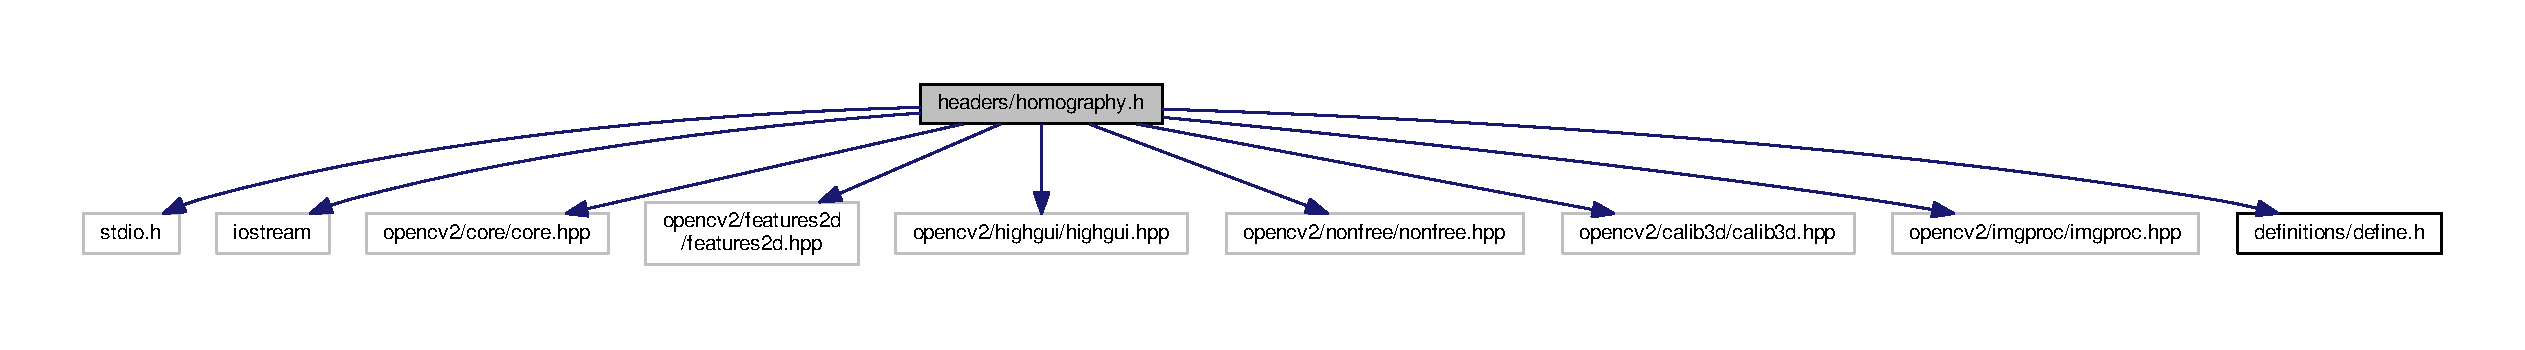
\includegraphics[width=350pt]{homography_8h__incl}
\end{center}
\end{figure}
This graph shows which files directly or indirectly include this file\+:\nopagebreak
\begin{figure}[H]
\begin{center}
\leavevmode
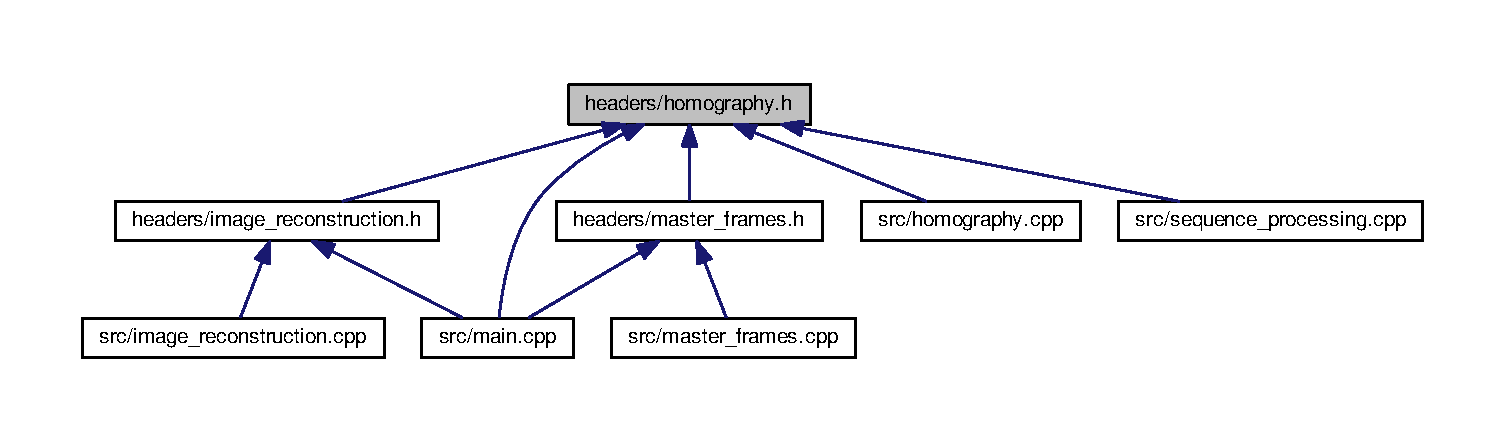
\includegraphics[width=350pt]{homography_8h__dep__incl}
\end{center}
\end{figure}
\subsection*{Enumerations}
\begin{DoxyCompactItemize}
\item 
enum \hyperlink{homography_8h_a340f89166e818e04b9c370262c161789}{Homog\+Coverage} \{ \hyperlink{homography_8h_a340f89166e818e04b9c370262c161789a552c25e928b15d492ee2e030f7645da6}{N\+O\+\_\+\+A\+R\+EA}, 
\hyperlink{homography_8h_a340f89166e818e04b9c370262c161789abe0b247460cf88426ab746417bd8cd3c}{D\+R\+O\+P\+\_\+\+A\+R\+EA}, 
\hyperlink{homography_8h_a340f89166e818e04b9c370262c161789a474302634cad5c69847b64b5f3160fef}{C\+R\+O\+P\+\_\+\+A\+R\+EA}
 \}\begin{DoxyCompactList}\small\item\em The Homog\+Coverage enum. \end{DoxyCompactList}
\end{DoxyCompactItemize}
\subsection*{Functions}
\begin{DoxyCompactItemize}
\item 
bool \hyperlink{homography_8h_a1d3798a81d0d3b5e8b24087a7bc60683}{find\+Homography\+Matrix} (const cv\+::\+Mat \&image\+\_\+src, const cv\+::\+Mat \&image\+\_\+dst, cv\+::\+Mat \&homography\+\_\+matrix, cv\+::\+Mat \&ransac\+\_\+mask)
\begin{DoxyCompactList}\small\item\em Function that find the homography matrix that leave the image\+Src to the plan of the image\+Dst. \end{DoxyCompactList}\item 
bool \hyperlink{homography_8h_a1bf28b8d881beac4a6deee5cbe7ae4da}{find\+Homography\+Matrix} (const cv\+::\+Mat \&image\+\_\+src, const cv\+::\+Mat \&image\+\_\+dst, cv\+::\+Mat \&homography\+\_\+matrix)
\begin{DoxyCompactList}\small\item\em Function that find the homography matrix that leave the image\+Src to the plan of the image\+Dst. \end{DoxyCompactList}\item 
bool \hyperlink{homography_8h_a3800765da624f694682f5f1fab7f4c63}{find\+Homography\+Matrix} (const std\+::vector$<$ cv\+::\+Key\+Point $>$ \&keypoints\+\_\+image\+\_\+src, const std\+::vector$<$ cv\+::\+Key\+Point $>$ \&keypoints\+\_\+image\+\_\+dst, const cv\+::\+Mat \&descriptors\+\_\+image\+\_\+src, const cv\+::\+Mat \&descriptors\+\_\+image\+\_\+dst, cv\+::\+Mat \&homography\+\_\+matrix, cv\+::\+Mat \&ransac\+\_\+mask)
\begin{DoxyCompactList}\small\item\em Function that finds the homography matrix given the keypoints and descriptors. \end{DoxyCompactList}\item 
bool \hyperlink{homography_8h_ae3833c553b4d2ea9817440dfc6f9b441}{find\+Homography\+Matrix} (const std\+::vector$<$ cv\+::\+Key\+Point $>$ \&keypoints\+\_\+image\+\_\+src, const std\+::vector$<$ cv\+::\+Key\+Point $>$ \&keypoints\+\_\+image\+\_\+dst, const cv\+::\+Mat \&descriptors\+\_\+image\+\_\+src, const cv\+::\+Mat \&descriptors\+\_\+image\+\_\+dst, cv\+::\+Mat \&homography\+\_\+matrix)
\begin{DoxyCompactList}\small\item\em Function that find the homography matrix that leaves the image\+Src to the plan of the image\+Dst. \end{DoxyCompactList}\item 
bool \hyperlink{homography_8h_af396adc4b5a19e8194e5ff96640f16de}{apply\+Homography\+Matrix} (const cv\+::\+Mat \&image\+\_\+src, const cv\+::\+Mat \&homography\+\_\+matrix, cv\+::\+Mat \&image\+\_\+result)
\begin{DoxyCompactList}\small\item\em Function that apply homography matrix in a given image. \end{DoxyCompactList}\item 
bool \hyperlink{homography_8h_a67a02c0cff3e126daece706c97c9ba2c}{check\+Homography\+Consistency} (const std\+::vector$<$ cv\+::\+Point2f $>$ img\+\_\+corners, const cv\+::\+Mat \&homography\+\_\+matrix)
\begin{DoxyCompactList}\small\item\em Function that checks if after made the homography transformation the corner consistency is maintained. \end{DoxyCompactList}\item 
bool \hyperlink{homography_8h_a3c17440ceb61568f04b508a4336c3402}{check\+Homography\+Consistency} (const std\+::vector$<$ cv\+::\+Point2f $>$ new\+\_\+img\+\_\+corners)
\begin{DoxyCompactList}\small\item\em Function that checks if after made the homography transformation the corner consistency is maintained. \end{DoxyCompactList}\item 
double \hyperlink{homography_8h_a94196b6d4321a287adf2b3051a5fad83}{get\+Area\+Ratio} (const cv\+::\+Mat \&image\+\_\+src, const cv\+::\+Mat \&homography\+\_\+matrix, const cv\+::\+Rect \&frame\+\_\+limits)
\begin{DoxyCompactList}\small\item\em Function that calculates the loss(\%) of the homography transformation in a R\+OI. \end{DoxyCompactList}\item 
\hyperlink{homography_8h_a340f89166e818e04b9c370262c161789}{Homog\+Coverage} \hyperlink{homography_8h_a8007547c4ef0394a46a61a21b6eab88c}{get\+Homog\+Coverage} (const cv\+::\+Mat \&image\+\_\+src, const cv\+::\+Mat \&homography\+\_\+matrix, const cv\+::\+Rect \&drop\+\_\+area, const cv\+::\+Rect \&crop\+\_\+area)
\begin{DoxyCompactList}\small\item\em Function that calculates the loss(\%) of the homography transformation in a R\+OI. \end{DoxyCompactList}\item 
void \hyperlink{homography_8h_af766393f5eb33e81f7f77f8ddc17cf03}{get\+Keypoints\+And\+Descriptors} (const cv\+::\+Mat \&image, std\+::vector$<$ cv\+::\+Key\+Point $>$ \&keypoints, cv\+::\+Mat \&descriptors)
\begin{DoxyCompactList}\small\item\em Function that gets the keypoints and describe an image in order to avoid unnecessary computations for tasks like finding the homography matrix. \end{DoxyCompactList}\end{DoxyCompactItemize}


\subsection{Detailed Description}
Header functions for the \hyperlink{homography_8cpp}{homography.\+cpp}. 



\subsection{Enumeration Type Documentation}
\index{homography.\+h@{homography.\+h}!Homog\+Coverage@{Homog\+Coverage}}
\index{Homog\+Coverage@{Homog\+Coverage}!homography.\+h@{homography.\+h}}
\subsubsection[{\texorpdfstring{Homog\+Coverage}{HomogCoverage}}]{\setlength{\rightskip}{0pt plus 5cm}enum {\bf Homog\+Coverage}}\hypertarget{homography_8h_a340f89166e818e04b9c370262c161789}{}\label{homography_8h_a340f89166e818e04b9c370262c161789}


The Homog\+Coverage enum. 

\begin{Desc}
\item[Enumerator]\par
\begin{description}
\index{N\+O\+\_\+\+A\+R\+EA@{N\+O\+\_\+\+A\+R\+EA}!homography.\+h@{homography.\+h}}\index{homography.\+h@{homography.\+h}!N\+O\+\_\+\+A\+R\+EA@{N\+O\+\_\+\+A\+R\+EA}}\item[{\em 
N\+O\+\_\+\+A\+R\+EA\hypertarget{homography_8h_a340f89166e818e04b9c370262c161789a552c25e928b15d492ee2e030f7645da6}{}\label{homography_8h_a340f89166e818e04b9c370262c161789a552c25e928b15d492ee2e030f7645da6}
}]\index{D\+R\+O\+P\+\_\+\+A\+R\+EA@{D\+R\+O\+P\+\_\+\+A\+R\+EA}!homography.\+h@{homography.\+h}}\index{homography.\+h@{homography.\+h}!D\+R\+O\+P\+\_\+\+A\+R\+EA@{D\+R\+O\+P\+\_\+\+A\+R\+EA}}\item[{\em 
D\+R\+O\+P\+\_\+\+A\+R\+EA\hypertarget{homography_8h_a340f89166e818e04b9c370262c161789abe0b247460cf88426ab746417bd8cd3c}{}\label{homography_8h_a340f89166e818e04b9c370262c161789abe0b247460cf88426ab746417bd8cd3c}
}]It can\textquotesingle{}t cover neither the drop area nor the crop area. \index{C\+R\+O\+P\+\_\+\+A\+R\+EA@{C\+R\+O\+P\+\_\+\+A\+R\+EA}!homography.\+h@{homography.\+h}}\index{homography.\+h@{homography.\+h}!C\+R\+O\+P\+\_\+\+A\+R\+EA@{C\+R\+O\+P\+\_\+\+A\+R\+EA}}\item[{\em 
C\+R\+O\+P\+\_\+\+A\+R\+EA\hypertarget{homography_8h_a340f89166e818e04b9c370262c161789a474302634cad5c69847b64b5f3160fef}{}\label{homography_8h_a340f89166e818e04b9c370262c161789a474302634cad5c69847b64b5f3160fef}
}]It covers the drop area, but doesn\textquotesingle{}t cover the crop area. It covers both the drop and the crop areas \end{description}
\end{Desc}


\subsection{Function Documentation}
\index{homography.\+h@{homography.\+h}!apply\+Homography\+Matrix@{apply\+Homography\+Matrix}}
\index{apply\+Homography\+Matrix@{apply\+Homography\+Matrix}!homography.\+h@{homography.\+h}}
\subsubsection[{\texorpdfstring{apply\+Homography\+Matrix(const cv\+::\+Mat \&image\+\_\+src, const cv\+::\+Mat \&homography\+\_\+matrix, cv\+::\+Mat \&image\+\_\+result)}{applyHomographyMatrix(const cv::Mat \&image\_src, const cv::Mat \&homography\_matrix, cv::Mat \&image\_result)}}]{\setlength{\rightskip}{0pt plus 5cm}bool apply\+Homography\+Matrix (
\begin{DoxyParamCaption}
\item[{const cv\+::\+Mat \&}]{image\+\_\+src, }
\item[{const cv\+::\+Mat \&}]{homography\+\_\+matrix, }
\item[{cv\+::\+Mat \&}]{image\+\_\+result}
\end{DoxyParamCaption}
)}\hypertarget{homography_8h_af396adc4b5a19e8194e5ff96640f16de}{}\label{homography_8h_af396adc4b5a19e8194e5ff96640f16de}


Function that apply homography matrix in a given image. 


\begin{DoxyParams}{Parameters}
{\em image\+\_\+src} & -\/ image where the homography matrix will be applied. \\
\hline
{\em homography\+\_\+matrix} & -\/ homography matrix. \\
\hline
{\em image\+\_\+result} & -\/ object to save the image after the application of the homography matrix.\\
\hline
\end{DoxyParams}
\begin{DoxyReturn}{Returns}
{\ttfamily bool} {\bfseries true} -\/ if the corner consistency is maintained after application of the homography matrix. ~\newline
 {\ttfamily bool} {\bfseries false} -\/ if the consistency is not maintained after application of the homography matrix. In this case the image\+Result is a simple copy of the image\+Src.
\end{DoxyReturn}
\begin{DoxyAuthor}{Author}
Michel Melo da Silva 
\end{DoxyAuthor}
\begin{DoxyDate}{Date}
25/03/2016 
\end{DoxyDate}
\index{homography.\+h@{homography.\+h}!check\+Homography\+Consistency@{check\+Homography\+Consistency}}
\index{check\+Homography\+Consistency@{check\+Homography\+Consistency}!homography.\+h@{homography.\+h}}
\subsubsection[{\texorpdfstring{check\+Homography\+Consistency(const std\+::vector$<$ cv\+::\+Point2f $>$ img\+\_\+corners, const cv\+::\+Mat \&homography\+\_\+matrix)}{checkHomographyConsistency(const std::vector< cv::Point2f > img\_corners, const cv::Mat \&homography\_matrix)}}]{\setlength{\rightskip}{0pt plus 5cm}bool check\+Homography\+Consistency (
\begin{DoxyParamCaption}
\item[{const std\+::vector$<$ cv\+::\+Point2f $>$}]{img\+\_\+corners, }
\item[{const cv\+::\+Mat \&}]{homography\+\_\+matrix}
\end{DoxyParamCaption}
)}\hypertarget{homography_8h_a67a02c0cff3e126daece706c97c9ba2c}{}\label{homography_8h_a67a02c0cff3e126daece706c97c9ba2c}


Function that checks if after made the homography transformation the corner consistency is maintained. 


\begin{DoxyParams}{Parameters}
{\em img\+\_\+corners} & -\/ image corners in the following order\+: ~\newline
 {\ttfamily img\+\_\+corners}\mbox{[}0\mbox{]} = 0 , 0 ~\newline
 {\ttfamily img\+\_\+corners}\mbox{[}1\mbox{]} = cols , 0 ~\newline
 {\ttfamily img\+\_\+corners}\mbox{[}2\mbox{]} = 0 , rows ~\newline
 {\ttfamily img\+\_\+corners}\mbox{[}3\mbox{]} = cols , rows \\
\hline
{\em homography\+\_\+matrix} & -\/ homography matrix that will be checked the consistency.\\
\hline
\end{DoxyParams}
\begin{DoxyReturn}{Returns}
{\ttfamily bool} {\bfseries true} -\/ if the consistency is maintained. ~\newline
 {\ttfamily bool} {\bfseries false} -\/ if the consistency is not maintained.
\end{DoxyReturn}
\begin{DoxyAuthor}{Author}
Michel Melo da Silva 
\end{DoxyAuthor}
\begin{DoxyDate}{Date}
08/04/2016 
\end{DoxyDate}
\index{homography.\+h@{homography.\+h}!check\+Homography\+Consistency@{check\+Homography\+Consistency}}
\index{check\+Homography\+Consistency@{check\+Homography\+Consistency}!homography.\+h@{homography.\+h}}
\subsubsection[{\texorpdfstring{check\+Homography\+Consistency(const std\+::vector$<$ cv\+::\+Point2f $>$ new\+\_\+img\+\_\+corners)}{checkHomographyConsistency(const std::vector< cv::Point2f > new\_img\_corners)}}]{\setlength{\rightskip}{0pt plus 5cm}bool check\+Homography\+Consistency (
\begin{DoxyParamCaption}
\item[{const std\+::vector$<$ cv\+::\+Point2f $>$}]{new\+\_\+img\+\_\+corners}
\end{DoxyParamCaption}
)}\hypertarget{homography_8h_a3c17440ceb61568f04b508a4336c3402}{}\label{homography_8h_a3c17440ceb61568f04b508a4336c3402}


Function that checks if after made the homography transformation the corner consistency is maintained. 


\begin{DoxyParams}{Parameters}
{\em new\+\_\+img\+\_\+corners} & -\/ image corners in the following order\+: ~\newline
 {\ttfamily img\+\_\+corners}\mbox{[}0\mbox{]} = 0 , 0 ~\newline
 {\ttfamily img\+\_\+corners}\mbox{[}1\mbox{]} = cols , 0 ~\newline
 {\ttfamily img\+\_\+corners}\mbox{[}2\mbox{]} = 0 , rows ~\newline
 {\ttfamily img\+\_\+corners}\mbox{[}3\mbox{]} = cols , rows\\
\hline
\end{DoxyParams}
\begin{DoxyReturn}{Returns}
{\ttfamily bool} {\bfseries true} -\/ if the consistency is maintained. ~\newline
 {\ttfamily bool} {\bfseries false} -\/ if the consistency is not maintained.
\end{DoxyReturn}
\begin{DoxyAuthor}{Author}
Michel Melo da Silva 
\end{DoxyAuthor}
\begin{DoxyDate}{Date}
12/04/2016 
\end{DoxyDate}
\index{homography.\+h@{homography.\+h}!find\+Homography\+Matrix@{find\+Homography\+Matrix}}
\index{find\+Homography\+Matrix@{find\+Homography\+Matrix}!homography.\+h@{homography.\+h}}
\subsubsection[{\texorpdfstring{find\+Homography\+Matrix(const cv\+::\+Mat \&image\+\_\+src, const cv\+::\+Mat \&image\+\_\+dst, cv\+::\+Mat \&homography\+\_\+matrix, cv\+::\+Mat \&ransac\+\_\+mask)}{findHomographyMatrix(const cv::Mat \&image\_src, const cv::Mat \&image\_dst, cv::Mat \&homography\_matrix, cv::Mat \&ransac\_mask)}}]{\setlength{\rightskip}{0pt plus 5cm}bool find\+Homography\+Matrix (
\begin{DoxyParamCaption}
\item[{const cv\+::\+Mat \&}]{image\+\_\+src, }
\item[{const cv\+::\+Mat \&}]{image\+\_\+dst, }
\item[{cv\+::\+Mat \&}]{homography\+\_\+matrix, }
\item[{cv\+::\+Mat \&}]{ransac\+\_\+mask}
\end{DoxyParamCaption}
)}\hypertarget{homography_8h_a1d3798a81d0d3b5e8b24087a7bc60683}{}\label{homography_8h_a1d3798a81d0d3b5e8b24087a7bc60683}


Function that find the homography matrix that leave the image\+Src to the plan of the image\+Dst. 

Returns the Ransak mask after finding the homography matrix.


\begin{DoxyParams}{Parameters}
{\em image\+\_\+src} & -\/ image to where the homography will be calculated. \\
\hline
{\em image\+\_\+dst} & -\/ image of the destination of the homography. \\
\hline
{\em homography\+\_\+matrix} & -\/ object to homography matrix calculated. \\
\hline
{\em ransac\+\_\+mask} & -\/ R\+A\+N\+S\+AC mask of the homography matrix. 1 means inliers and 0 means outliers.\\
\hline
\end{DoxyParams}
\begin{DoxyReturn}{Returns}
{\ttfamily bool} {\bfseries true} -\/ if there is enough points in both images and good matches between them to find a homography matrix. ~\newline
 {\ttfamily bool} {\bfseries false} -\/ if there is not enough points in both images or good matches between them to find a homography matrix.
\end{DoxyReturn}
\begin{DoxyAuthor}{Author}
Michel Melo da Silva 
\end{DoxyAuthor}
\begin{DoxyDate}{Date}
28/03/2016
\end{DoxyDate}
Function that find the homography matrix that leave the image\+Src to the plan of the image\+Dst.

Returns the Ransak mask after finding the homography matrix.


\begin{DoxyParams}{Parameters}
{\em image\+\_\+src} & -\/ image to where the homography will be calculated. \\
\hline
{\em image\+\_\+dst} & -\/ image of the destination of the homography. \\
\hline
{\em homography\+\_\+matrix} & -\/ object to homography matrix calculated. \\
\hline
{\em ransac\+\_\+mask} & -\/ R\+A\+N\+S\+AC mask of the homography matrix. 1 means inliers and 0 means outliers.\\
\hline
\end{DoxyParams}
\begin{DoxyReturn}{Returns}
{\ttfamily bool} {\bfseries true} -\/ if there is enough points in both images and good matches between them to find a homography matrix. ~\newline
 {\ttfamily bool} {\bfseries false} -\/ if there is not enough points in both images or good matches between them to find a homography matrix.
\end{DoxyReturn}
\begin{DoxyAuthor}{Author}
Michel Melo da Silva 
\end{DoxyAuthor}
\begin{DoxyDate}{Date}
28/03/2016 
\end{DoxyDate}
\index{homography.\+h@{homography.\+h}!find\+Homography\+Matrix@{find\+Homography\+Matrix}}
\index{find\+Homography\+Matrix@{find\+Homography\+Matrix}!homography.\+h@{homography.\+h}}
\subsubsection[{\texorpdfstring{find\+Homography\+Matrix(const cv\+::\+Mat \&image\+\_\+src, const cv\+::\+Mat \&image\+\_\+dst, cv\+::\+Mat \&homography\+\_\+matrix)}{findHomographyMatrix(const cv::Mat \&image\_src, const cv::Mat \&image\_dst, cv::Mat \&homography\_matrix)}}]{\setlength{\rightskip}{0pt plus 5cm}bool find\+Homography\+Matrix (
\begin{DoxyParamCaption}
\item[{const cv\+::\+Mat \&}]{image\+\_\+src, }
\item[{const cv\+::\+Mat \&}]{image\+\_\+dst, }
\item[{cv\+::\+Mat \&}]{homography\+\_\+matrix}
\end{DoxyParamCaption}
)}\hypertarget{homography_8h_a1bf28b8d881beac4a6deee5cbe7ae4da}{}\label{homography_8h_a1bf28b8d881beac4a6deee5cbe7ae4da}


Function that find the homography matrix that leave the image\+Src to the plan of the image\+Dst. 


\begin{DoxyParams}{Parameters}
{\em image\+\_\+src} & -\/ image to where the homography will be calculated. \\
\hline
{\em image\+\_\+dst} & -\/ image of the destination of the homography. \\
\hline
{\em homography\+\_\+matrix} & -\/ object to save the homography matrix calculated.\\
\hline
\end{DoxyParams}
\begin{DoxyReturn}{Returns}
{\ttfamily bool} {\bfseries true} -\/ if there is enough points in both images and good matches between them to find a homography matrix. ~\newline
 {\ttfamily bool} {\bfseries false} -\/ if there is not enough points in both images or good matches between them to find a homography matrix.
\end{DoxyReturn}
\begin{DoxyAuthor}{Author}
Michel Melo da Silva 
\end{DoxyAuthor}
\begin{DoxyDate}{Date}
28/03/2016
\end{DoxyDate}
Function that find the homography matrix that leave the image\+Src to the plan of the image\+Dst.


\begin{DoxyParams}{Parameters}
{\em image\+\_\+src} & -\/ image to where the homography will be calculated. \\
\hline
{\em image\+\_\+dst} & -\/ image of the destination of the homography. \\
\hline
{\em homography\+\_\+matrix} & -\/ object to save the homography matrix calculated.\\
\hline
\end{DoxyParams}
\begin{DoxyReturn}{Returns}
{\ttfamily bool} {\bfseries true} -\/ if there is enough points in both images and good matches between them to find a homography matrix. ~\newline
 {\ttfamily bool} {\bfseries false} -\/ if there is not enough points in both images or good matches between them to find a homography matrix.
\end{DoxyReturn}
\begin{DoxyAuthor}{Author}
Michel Melo da Silva 
\end{DoxyAuthor}
\begin{DoxyDate}{Date}
28/03/2016 
\end{DoxyDate}
\index{homography.\+h@{homography.\+h}!find\+Homography\+Matrix@{find\+Homography\+Matrix}}
\index{find\+Homography\+Matrix@{find\+Homography\+Matrix}!homography.\+h@{homography.\+h}}
\subsubsection[{\texorpdfstring{find\+Homography\+Matrix(const std\+::vector$<$ cv\+::\+Key\+Point $>$ \&keypoints\+\_\+image\+\_\+src, const std\+::vector$<$ cv\+::\+Key\+Point $>$ \&keypoints\+\_\+image\+\_\+dst, const cv\+::\+Mat \&descriptors\+\_\+image\+\_\+src, const cv\+::\+Mat \&descriptors\+\_\+image\+\_\+dst, cv\+::\+Mat \&homography\+\_\+matrix, cv\+::\+Mat \&ransac\+\_\+mask)}{findHomographyMatrix(const std::vector< cv::KeyPoint > \&keypoints\_image\_src, const std::vector< cv::KeyPoint > \&keypoints\_image\_dst, const cv::Mat \&descriptors\_image\_src, const cv::Mat \&descriptors\_image\_dst, cv::Mat \&homography\_matrix, cv::Mat \&ransac\_mask)}}]{\setlength{\rightskip}{0pt plus 5cm}bool find\+Homography\+Matrix (
\begin{DoxyParamCaption}
\item[{const std\+::vector$<$ cv\+::\+Key\+Point $>$ \&}]{keypoints\+\_\+image\+\_\+src, }
\item[{const std\+::vector$<$ cv\+::\+Key\+Point $>$ \&}]{keypoints\+\_\+image\+\_\+dst, }
\item[{const cv\+::\+Mat \&}]{descriptors\+\_\+image\+\_\+src, }
\item[{const cv\+::\+Mat \&}]{descriptors\+\_\+image\+\_\+dst, }
\item[{cv\+::\+Mat \&}]{homography\+\_\+matrix, }
\item[{cv\+::\+Mat \&}]{ransac\+\_\+mask}
\end{DoxyParamCaption}
)}\hypertarget{homography_8h_a3800765da624f694682f5f1fab7f4c63}{}\label{homography_8h_a3800765da624f694682f5f1fab7f4c63}


Function that finds the homography matrix given the keypoints and descriptors. 

Returns the Ransak mask after finding the homography matrix.


\begin{DoxyParams}{Parameters}
{\em keypoints\+\_\+image\+\_\+src} & -\/ keypoints of the source image. \\
\hline
{\em keypoints\+\_\+image\+\_\+dst} & -\/ keypoints of the target image. \\
\hline
{\em descriptors\+\_\+image\+\_\+src} & -\/ descriptors of the source image. \\
\hline
{\em descriptors\+\_\+image\+\_\+dst} & -\/ descriptors of the target image. \\
\hline
{\em homography\+\_\+matrix} & -\/ object to homography matrix calculated. \\
\hline
{\em ransac\+\_\+mask} & -\/ R\+A\+N\+S\+AC mask of the homography matrix. 1 means inliers and 0 means outliers.\\
\hline
\end{DoxyParams}
\begin{DoxyReturn}{Returns}
{\ttfamily bool} {\bfseries true} -\/ if there is enough points in both images and good matches between them to find a homography matrix. ~\newline
 {\ttfamily bool} {\bfseries false} -\/ if there is not enough points in both images or good matches between them to find a homography matrix.
\end{DoxyReturn}
\begin{DoxyAuthor}{Author}
Washington Luis de Souza Ramos 
\end{DoxyAuthor}
\begin{DoxyDate}{Date}
30/08/2016 
\end{DoxyDate}
\index{homography.\+h@{homography.\+h}!find\+Homography\+Matrix@{find\+Homography\+Matrix}}
\index{find\+Homography\+Matrix@{find\+Homography\+Matrix}!homography.\+h@{homography.\+h}}
\subsubsection[{\texorpdfstring{find\+Homography\+Matrix(const std\+::vector$<$ cv\+::\+Key\+Point $>$ \&keypoints\+\_\+image\+\_\+src, const std\+::vector$<$ cv\+::\+Key\+Point $>$ \&keypoints\+\_\+image\+\_\+dst, const cv\+::\+Mat \&descriptors\+\_\+image\+\_\+src, const cv\+::\+Mat \&descriptors\+\_\+image\+\_\+dst, cv\+::\+Mat \&homography\+\_\+matrix)}{findHomographyMatrix(const std::vector< cv::KeyPoint > \&keypoints\_image\_src, const std::vector< cv::KeyPoint > \&keypoints\_image\_dst, const cv::Mat \&descriptors\_image\_src, const cv::Mat \&descriptors\_image\_dst, cv::Mat \&homography\_matrix)}}]{\setlength{\rightskip}{0pt plus 5cm}bool find\+Homography\+Matrix (
\begin{DoxyParamCaption}
\item[{const std\+::vector$<$ cv\+::\+Key\+Point $>$ \&}]{keypoints\+\_\+image\+\_\+src, }
\item[{const std\+::vector$<$ cv\+::\+Key\+Point $>$ \&}]{keypoints\+\_\+image\+\_\+dst, }
\item[{const cv\+::\+Mat \&}]{descriptors\+\_\+image\+\_\+src, }
\item[{const cv\+::\+Mat \&}]{descriptors\+\_\+image\+\_\+dst, }
\item[{cv\+::\+Mat \&}]{homography\+\_\+matrix}
\end{DoxyParamCaption}
)}\hypertarget{homography_8h_ae3833c553b4d2ea9817440dfc6f9b441}{}\label{homography_8h_ae3833c553b4d2ea9817440dfc6f9b441}


Function that find the homography matrix that leaves the image\+Src to the plan of the image\+Dst. 


\begin{DoxyParams}{Parameters}
{\em keypoints\+\_\+image\+\_\+src} & -\/ keypoints of the source image. \\
\hline
{\em keypoints\+\_\+image\+\_\+dst} & -\/ keypoints of the target image. \\
\hline
{\em descriptors\+\_\+image\+\_\+src} & -\/ descriptors of the source image. \\
\hline
{\em descriptors\+\_\+image\+\_\+dst} & -\/ descriptors of the target image. \\
\hline
{\em homography\+\_\+matrix} & -\/ object to save the homography matrix calculated.\\
\hline
\end{DoxyParams}
\begin{DoxyReturn}{Returns}
{\ttfamily bool} {\bfseries true} -\/ if there is enough points in both images and good matches between them to find a homography matrix. ~\newline
 {\ttfamily bool} {\bfseries false} -\/ if there is not enough points in both images or good matches between them to find a homography matrix.
\end{DoxyReturn}
\begin{DoxyAuthor}{Author}
Washington Luis de Souza Ramos 
\end{DoxyAuthor}
\begin{DoxyDate}{Date}
09/09/2016 
\end{DoxyDate}
\index{homography.\+h@{homography.\+h}!get\+Area\+Ratio@{get\+Area\+Ratio}}
\index{get\+Area\+Ratio@{get\+Area\+Ratio}!homography.\+h@{homography.\+h}}
\subsubsection[{\texorpdfstring{get\+Area\+Ratio(const cv\+::\+Mat \&image\+\_\+src, const cv\+::\+Mat \&homography\+\_\+matrix, const cv\+::\+Rect \&frame\+\_\+limits)}{getAreaRatio(const cv::Mat \&image\_src, const cv::Mat \&homography\_matrix, const cv::Rect \&frame\_limits)}}]{\setlength{\rightskip}{0pt plus 5cm}double get\+Area\+Ratio (
\begin{DoxyParamCaption}
\item[{const cv\+::\+Mat \&}]{image\+\_\+src, }
\item[{const cv\+::\+Mat \&}]{homography\+\_\+matrix, }
\item[{const cv\+::\+Rect \&}]{frame\+\_\+limits}
\end{DoxyParamCaption}
)}\hypertarget{homography_8h_a94196b6d4321a287adf2b3051a5fad83}{}\label{homography_8h_a94196b6d4321a287adf2b3051a5fad83}


Function that calculates the loss(\%) of the homography transformation in a R\+OI. 

It returns the ratio between the non-\/image area and the frame\+\_\+limits area.


\begin{DoxyParams}{Parameters}
{\em image\+\_\+src} & -\/ The source image. \\
\hline
{\em homography\+\_\+matrix} & -\/ The homography matrix. \\
\hline
{\em frame\+\_\+limits} & -\/ The region of interest (R\+OI).\\
\hline
\end{DoxyParams}
\begin{DoxyReturn}{Returns}
{\ttfamily double} -\/ The ratio between non-\/image area and the whole frame area.
\end{DoxyReturn}
\begin{DoxyAuthor}{Author}
Washington Luis de Souza Ramos 
\end{DoxyAuthor}
\begin{DoxyDate}{Date}
14/04/2016 
\end{DoxyDate}
\index{homography.\+h@{homography.\+h}!get\+Homog\+Coverage@{get\+Homog\+Coverage}}
\index{get\+Homog\+Coverage@{get\+Homog\+Coverage}!homography.\+h@{homography.\+h}}
\subsubsection[{\texorpdfstring{get\+Homog\+Coverage(const cv\+::\+Mat \&image\+\_\+src, const cv\+::\+Mat \&homography\+\_\+matrix, const cv\+::\+Rect \&drop\+\_\+area, const cv\+::\+Rect \&crop\+\_\+area)}{getHomogCoverage(const cv::Mat \&image\_src, const cv::Mat \&homography\_matrix, const cv::Rect \&drop\_area, const cv::Rect \&crop\_area)}}]{\setlength{\rightskip}{0pt plus 5cm}{\bf Homog\+Coverage} get\+Homog\+Coverage (
\begin{DoxyParamCaption}
\item[{const cv\+::\+Mat \&}]{image\+\_\+src, }
\item[{const cv\+::\+Mat \&}]{homography\+\_\+matrix, }
\item[{const cv\+::\+Rect \&}]{drop\+\_\+area, }
\item[{const cv\+::\+Rect \&}]{crop\+\_\+area}
\end{DoxyParamCaption}
)}\hypertarget{homography_8h_a8007547c4ef0394a46a61a21b6eab88c}{}\label{homography_8h_a8007547c4ef0394a46a61a21b6eab88c}


Function that calculates the loss(\%) of the homography transformation in a R\+OI. 

It returns the coverage of a transformation which is N\+O\+NE, D\+R\+O\+P\+\_\+\+A\+R\+EA or C\+R\+O\+P\+\_\+\+A\+R\+EA. 
\begin{DoxyParams}{Parameters}
{\em image\+\_\+src} & -\/ The source image. \\
\hline
{\em homography\+\_\+matrix} & -\/ The homography matrix. \\
\hline
{\em drop\+\_\+area} & -\/ The region of interest (R\+OI) for the drop area. \\
\hline
{\em crop\+\_\+area} & -\/ The region of interest (R\+OI) for the crop area. \\
\hline
\end{DoxyParams}
\begin{DoxyReturn}{Returns}
The Homog\+Coverage enum value
\end{DoxyReturn}
\begin{DoxyAuthor}{Author}
Washington Luis de Souza Ramos 
\end{DoxyAuthor}
\begin{DoxyDate}{Date}
10/09/2016 
\end{DoxyDate}
\index{homography.\+h@{homography.\+h}!get\+Keypoints\+And\+Descriptors@{get\+Keypoints\+And\+Descriptors}}
\index{get\+Keypoints\+And\+Descriptors@{get\+Keypoints\+And\+Descriptors}!homography.\+h@{homography.\+h}}
\subsubsection[{\texorpdfstring{get\+Keypoints\+And\+Descriptors(const cv\+::\+Mat \&image, std\+::vector$<$ cv\+::\+Key\+Point $>$ \&keypoints, cv\+::\+Mat \&descriptors)}{getKeypointsAndDescriptors(const cv::Mat \&image, std::vector< cv::KeyPoint > \&keypoints, cv::Mat \&descriptors)}}]{\setlength{\rightskip}{0pt plus 5cm}void get\+Keypoints\+And\+Descriptors (
\begin{DoxyParamCaption}
\item[{const cv\+::\+Mat \&}]{image, }
\item[{std\+::vector$<$ cv\+::\+Key\+Point $>$ \&}]{keypoints, }
\item[{cv\+::\+Mat \&}]{descriptors}
\end{DoxyParamCaption}
)}\hypertarget{homography_8h_af766393f5eb33e81f7f77f8ddc17cf03}{}\label{homography_8h_af766393f5eb33e81f7f77f8ddc17cf03}


Function that gets the keypoints and describe an image in order to avoid unnecessary computations for tasks like finding the homography matrix. 


\begin{DoxyParams}{Parameters}
{\em image} & -\/ image to where the keypoints and descriptors are to be extracted from. \\
\hline
{\em keypoints} & -\/ the keypoints found in the image. \\
\hline
{\em descriptors} & -\/ the descriptors of the image.\\
\hline
\end{DoxyParams}
\begin{DoxyAuthor}{Author}
Washington Luis de Souza Ramos 
\end{DoxyAuthor}
\begin{DoxyDate}{Date}
30/08/2016 
\end{DoxyDate}

\hypertarget{image__reconstruction_8h}{}\section{headers/image\+\_\+reconstruction.h File Reference}
\label{image__reconstruction_8h}\index{headers/image\+\_\+reconstruction.\+h@{headers/image\+\_\+reconstruction.\+h}}


Header functions for the \hyperlink{image__reconstruction_8cpp}{image\+\_\+reconstruction.\+cpp}.  


{\ttfamily \#include $<$stdio.\+h$>$}\\*
{\ttfamily \#include $<$iostream$>$}\\*
{\ttfamily \#include $<$opencv2/core/core.\+hpp$>$}\\*
{\ttfamily \#include $<$opencv2/features2d/features2d.\+hpp$>$}\\*
{\ttfamily \#include $<$opencv2/highgui/highgui.\+hpp$>$}\\*
{\ttfamily \#include $<$opencv2/nonfree/nonfree.\+hpp$>$}\\*
{\ttfamily \#include $<$opencv2/calib3d/calib3d.\+hpp$>$}\\*
{\ttfamily \#include $<$opencv2/imgproc/imgproc.\+hpp$>$}\\*
{\ttfamily \#include $<$opencv2/photo/photo.\+hpp$>$}\\*
{\ttfamily \#include \char`\"{}definitions/define.\+h\char`\"{}}\\*
{\ttfamily \#include \char`\"{}definitions/experiment\+\_\+struct.\+h\char`\"{}}\\*
{\ttfamily \#include \char`\"{}executables/execute\+\_\+commands.\+h\char`\"{}}\\*
{\ttfamily \#include \char`\"{}homography.\+h\char`\"{}}\\*
Include dependency graph for image\+\_\+reconstruction.\+h\+:\nopagebreak
\begin{figure}[H]
\begin{center}
\leavevmode
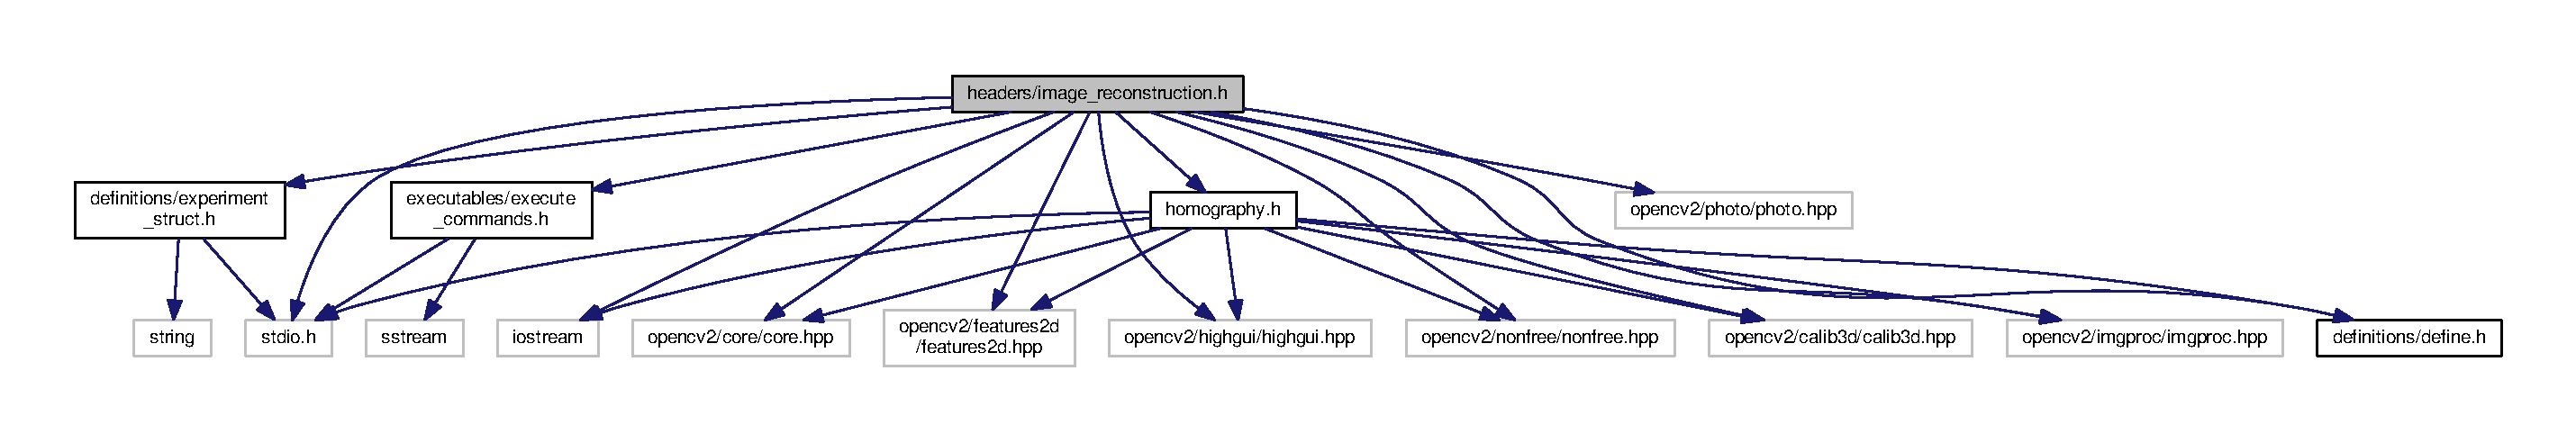
\includegraphics[width=350pt]{image__reconstruction_8h__incl}
\end{center}
\end{figure}
This graph shows which files directly or indirectly include this file\+:\nopagebreak
\begin{figure}[H]
\begin{center}
\leavevmode
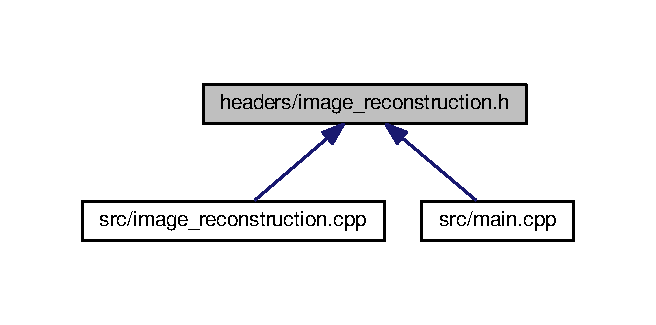
\includegraphics[width=315pt]{image__reconstruction_8h__dep__incl}
\end{center}
\end{figure}
\subsection*{Enumerations}
\begin{DoxyCompactItemize}
\item 
enum \hyperlink{image__reconstruction_8h_ad5c30c75ffcd2ccec3fad8a118addb15}{Reconstruction\+Type} \{ \hyperlink{image__reconstruction_8h_ad5c30c75ffcd2ccec3fad8a118addb15a24c4f661ea927ff88a09e2d2c44cfc0f}{P\+R\+E\+\_\+\+A\+N\+D\+\_\+\+P\+OS}, 
\hyperlink{image__reconstruction_8h_ad5c30c75ffcd2ccec3fad8a118addb15a7b2b01785df1bdd40fec44c53d0011f8}{O\+N\+L\+Y\+\_\+\+P\+RE}, 
\hyperlink{image__reconstruction_8h_ad5c30c75ffcd2ccec3fad8a118addb15a54c8830522aa455e2a777ccd97b0cecc}{O\+N\+L\+Y\+\_\+\+P\+OS}
 \}
\end{DoxyCompactItemize}
\subsection*{Functions}
\begin{DoxyCompactItemize}
\item 
bool \hyperlink{image__reconstruction_8h_aa59aa1053c00066ff2e977650615393d}{image\+Reconstruction} (const cv\+::\+Mat \&image, const int index, const \hyperlink{structEXPERIMENT}{E\+X\+P\+E\+R\+I\+M\+E\+NT} \&\hyperlink{main_8cpp_a9f5a81402e170475690f371d55cbe623}{experiment\+\_\+settings}, const cv\+::\+Rect \&frame\+\_\+boundaries, cv\+::\+Mat \&reconstructed\+Image)
\begin{DoxyCompactList}\small\item\em Function that reconstructs an image using panorama based on homography in a image sequence. \end{DoxyCompactList}\item 
bool \hyperlink{image__reconstruction_8h_ad6b2680d1178aa193da11f5173c40c3c}{reconstruct\+Image} (const cv\+::\+Mat \&image, const cv\+::\+Mat \&homography\+\_\+matrix, const int index, const \hyperlink{structEXPERIMENT}{E\+X\+P\+E\+R\+I\+M\+E\+NT} \&\hyperlink{main_8cpp_a9f5a81402e170475690f371d55cbe623}{experiment\+\_\+settings}, const cv\+::\+Rect \&drop\+\_\+boundaries, const cv\+::\+Rect \&frame\+\_\+boundaries, cv\+::\+Mat \&reconstructed\+\_\+image)
\begin{DoxyCompactList}\small\item\em Function that reconstructs an image using panorama based on homography in a image sequence. \end{DoxyCompactList}\end{DoxyCompactItemize}


\subsection{Detailed Description}
Header functions for the \hyperlink{image__reconstruction_8cpp}{image\+\_\+reconstruction.\+cpp}. 



\subsection{Enumeration Type Documentation}
\index{image\+\_\+reconstruction.\+h@{image\+\_\+reconstruction.\+h}!Reconstruction\+Type@{Reconstruction\+Type}}
\index{Reconstruction\+Type@{Reconstruction\+Type}!image\+\_\+reconstruction.\+h@{image\+\_\+reconstruction.\+h}}
\subsubsection[{\texorpdfstring{Reconstruction\+Type}{ReconstructionType}}]{\setlength{\rightskip}{0pt plus 5cm}enum {\bf Reconstruction\+Type}}\hypertarget{image__reconstruction_8h_ad5c30c75ffcd2ccec3fad8a118addb15}{}\label{image__reconstruction_8h_ad5c30c75ffcd2ccec3fad8a118addb15}
\begin{Desc}
\item[Enumerator]\par
\begin{description}
\index{P\+R\+E\+\_\+\+A\+N\+D\+\_\+\+P\+OS@{P\+R\+E\+\_\+\+A\+N\+D\+\_\+\+P\+OS}!image\+\_\+reconstruction.\+h@{image\+\_\+reconstruction.\+h}}\index{image\+\_\+reconstruction.\+h@{image\+\_\+reconstruction.\+h}!P\+R\+E\+\_\+\+A\+N\+D\+\_\+\+P\+OS@{P\+R\+E\+\_\+\+A\+N\+D\+\_\+\+P\+OS}}\item[{\em 
P\+R\+E\+\_\+\+A\+N\+D\+\_\+\+P\+OS\hypertarget{image__reconstruction_8h_ad5c30c75ffcd2ccec3fad8a118addb15a24c4f661ea927ff88a09e2d2c44cfc0f}{}\label{image__reconstruction_8h_ad5c30c75ffcd2ccec3fad8a118addb15a24c4f661ea927ff88a09e2d2c44cfc0f}
}]\index{O\+N\+L\+Y\+\_\+\+P\+RE@{O\+N\+L\+Y\+\_\+\+P\+RE}!image\+\_\+reconstruction.\+h@{image\+\_\+reconstruction.\+h}}\index{image\+\_\+reconstruction.\+h@{image\+\_\+reconstruction.\+h}!O\+N\+L\+Y\+\_\+\+P\+RE@{O\+N\+L\+Y\+\_\+\+P\+RE}}\item[{\em 
O\+N\+L\+Y\+\_\+\+P\+RE\hypertarget{image__reconstruction_8h_ad5c30c75ffcd2ccec3fad8a118addb15a7b2b01785df1bdd40fec44c53d0011f8}{}\label{image__reconstruction_8h_ad5c30c75ffcd2ccec3fad8a118addb15a7b2b01785df1bdd40fec44c53d0011f8}
}]\index{O\+N\+L\+Y\+\_\+\+P\+OS@{O\+N\+L\+Y\+\_\+\+P\+OS}!image\+\_\+reconstruction.\+h@{image\+\_\+reconstruction.\+h}}\index{image\+\_\+reconstruction.\+h@{image\+\_\+reconstruction.\+h}!O\+N\+L\+Y\+\_\+\+P\+OS@{O\+N\+L\+Y\+\_\+\+P\+OS}}\item[{\em 
O\+N\+L\+Y\+\_\+\+P\+OS\hypertarget{image__reconstruction_8h_ad5c30c75ffcd2ccec3fad8a118addb15a54c8830522aa455e2a777ccd97b0cecc}{}\label{image__reconstruction_8h_ad5c30c75ffcd2ccec3fad8a118addb15a54c8830522aa455e2a777ccd97b0cecc}
}]\end{description}
\end{Desc}


\subsection{Function Documentation}
\index{image\+\_\+reconstruction.\+h@{image\+\_\+reconstruction.\+h}!image\+Reconstruction@{image\+Reconstruction}}
\index{image\+Reconstruction@{image\+Reconstruction}!image\+\_\+reconstruction.\+h@{image\+\_\+reconstruction.\+h}}
\subsubsection[{\texorpdfstring{image\+Reconstruction(const cv\+::\+Mat \&image, const int index, const E\+X\+P\+E\+R\+I\+M\+E\+N\+T \&experiment\+\_\+settings, const cv\+::\+Rect \&frame\+\_\+boundaries, cv\+::\+Mat \&reconstructed\+Image)}{imageReconstruction(const cv::Mat \&image, const int index, const EXPERIMENT \&experiment\_settings, const cv::Rect \&frame\_boundaries, cv::Mat \&reconstructedImage)}}]{\setlength{\rightskip}{0pt plus 5cm}bool image\+Reconstruction (
\begin{DoxyParamCaption}
\item[{const cv\+::\+Mat \&}]{image, }
\item[{const int}]{index, }
\item[{const {\bf E\+X\+P\+E\+R\+I\+M\+E\+NT} \&}]{experiment\+\_\+settings, }
\item[{const cv\+::\+Rect \&}]{frame\+\_\+boundaries, }
\item[{cv\+::\+Mat \&}]{reconstructed\+\_\+image}
\end{DoxyParamCaption}
)}\hypertarget{image__reconstruction_8h_aa59aa1053c00066ff2e977650615393d}{}\label{image__reconstruction_8h_aa59aa1053c00066ff2e977650615393d}


Function that reconstructs an image using panorama based on homography in a image sequence. 


\begin{DoxyParams}{Parameters}
{\em image} & -\/ image initial with homography transformation. \\
\hline
{\em index} & -\/ index of the initial image in the original video. \\
\hline
{\em experiment\+\_\+settings} & -\/ object with the experiment settings. \\
\hline
{\em frame\+\_\+boundaries} & -\/ limits of the frame that needs to be filled by the reconstructed image. \\
\hline
{\em reconstructed\+\_\+image} & -\/ object to save the final reconstructed image.\\
\hline
\end{DoxyParams}
\begin{DoxyReturn}{Returns}
{\ttfamily bool} {\bfseries true} -\/ if the frame was successful reconstructed filling all the frame limit. ~\newline
 {\ttfamily bool} {\bfseries false} -\/ if the frame was not successful reconstructed filling all the frame limit.
\end{DoxyReturn}
\begin{DoxyAuthor}{Author}
Michel Melo da Silva 
\end{DoxyAuthor}
\begin{DoxyDate}{Date}
14/04/2016 
\end{DoxyDate}
\index{image\+\_\+reconstruction.\+h@{image\+\_\+reconstruction.\+h}!reconstruct\+Image@{reconstruct\+Image}}
\index{reconstruct\+Image@{reconstruct\+Image}!image\+\_\+reconstruction.\+h@{image\+\_\+reconstruction.\+h}}
\subsubsection[{\texorpdfstring{reconstruct\+Image(const cv\+::\+Mat \&image, const cv\+::\+Mat \&homography\+\_\+matrix, const int index, const E\+X\+P\+E\+R\+I\+M\+E\+N\+T \&experiment\+\_\+settings, const cv\+::\+Rect \&drop\+\_\+boundaries, const cv\+::\+Rect \&frame\+\_\+boundaries, cv\+::\+Mat \&reconstructed\+\_\+image)}{reconstructImage(const cv::Mat \&image, const cv::Mat \&homography\_matrix, const int index, const EXPERIMENT \&experiment\_settings, const cv::Rect \&drop\_boundaries, const cv::Rect \&frame\_boundaries, cv::Mat \&reconstructed\_image)}}]{\setlength{\rightskip}{0pt plus 5cm}bool reconstruct\+Image (
\begin{DoxyParamCaption}
\item[{const cv\+::\+Mat \&}]{image, }
\item[{const cv\+::\+Mat \&}]{homography\+\_\+matrix, }
\item[{const int}]{index, }
\item[{const {\bf E\+X\+P\+E\+R\+I\+M\+E\+NT} \&}]{experiment\+\_\+settings, }
\item[{const cv\+::\+Rect \&}]{drop\+\_\+boundaries, }
\item[{const cv\+::\+Rect \&}]{frame\+\_\+boundaries, }
\item[{cv\+::\+Mat \&}]{reconstructed\+\_\+image}
\end{DoxyParamCaption}
)}\hypertarget{image__reconstruction_8h_ad6b2680d1178aa193da11f5173c40c3c}{}\label{image__reconstruction_8h_ad6b2680d1178aa193da11f5173c40c3c}


Function that reconstructs an image using panorama based on homography in a image sequence. 


\begin{DoxyParams}{Parameters}
{\em image} & -\/ image initial without homography transformation. \\
\hline
{\em homography\+\_\+matrix} & -\/ homography matrix that will be applied to the original image where the reconstruct will start. \\
\hline
{\em index} & -\/ index of the initial image in the original video. \\
\hline
{\em experiment\+\_\+settings} & -\/ object with the experiment settings. \\
\hline
{\em frame\+\_\+boundaries} & -\/ limits of the frame that needs to be filled by the reconstructed image. \\
\hline
{\em reconstructed\+\_\+image} & -\/ object to save the final reconstructed image.\\
\hline
\end{DoxyParams}
\begin{DoxyReturn}{Returns}
{\ttfamily bool} {\bfseries true} -\/ if the frame was successful reconstructed filling all the frame limit. ~\newline
 {\ttfamily bool} {\bfseries false} -\/ if the frame was not successful reconstructed filling all the frame limit.
\end{DoxyReturn}
\begin{DoxyAuthor}{Author}
Michel Melo da Silva 
\end{DoxyAuthor}
\begin{DoxyDate}{Date}
14/04/2016 
\end{DoxyDate}

\hypertarget{line__and__point__operations_8h}{}\section{headers/line\+\_\+and\+\_\+point\+\_\+operations.h File Reference}
\label{line__and__point__operations_8h}\index{headers/line\+\_\+and\+\_\+point\+\_\+operations.\+h@{headers/line\+\_\+and\+\_\+point\+\_\+operations.\+h}}


Header functions for the \hyperlink{line__and__point__operations_8cpp}{line\+\_\+and\+\_\+point\+\_\+operations.\+cpp}.  


{\ttfamily \#include $<$stdio.\+h$>$}\\*
{\ttfamily \#include $<$iostream$>$}\\*
{\ttfamily \#include $<$opencv2/core/core.\+hpp$>$}\\*
{\ttfamily \#include $<$opencv2/highgui/highgui.\+hpp$>$}\\*
{\ttfamily \#include $<$opencv2/imgproc/imgproc.\+hpp$>$}\\*
Include dependency graph for line\+\_\+and\+\_\+point\+\_\+operations.\+h\+:\nopagebreak
\begin{figure}[H]
\begin{center}
\leavevmode
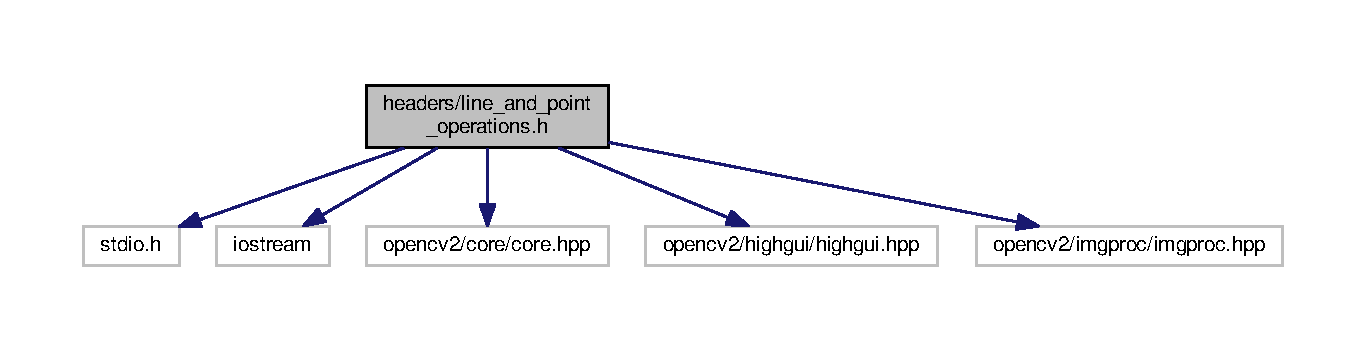
\includegraphics[width=350pt]{line__and__point__operations_8h__incl}
\end{center}
\end{figure}
This graph shows which files directly or indirectly include this file\+:\nopagebreak
\begin{figure}[H]
\begin{center}
\leavevmode
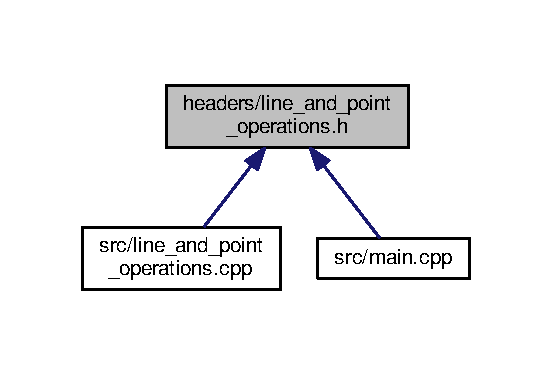
\includegraphics[width=265pt]{line__and__point__operations_8h__dep__incl}
\end{center}
\end{figure}
\subsection*{Macros}
\begin{DoxyCompactItemize}
\item 
\#define \hyperlink{line__and__point__operations_8h_a002b2f4894492820fe708b1b7e7c5e70}{E\+P\+S\+I\+L\+ON}~1\+E-\/5
\begin{DoxyCompactList}\small\item\em Maximum difference to consider two values equals. \end{DoxyCompactList}\end{DoxyCompactItemize}
\subsection*{Functions}
\begin{DoxyCompactItemize}
\item 
bool \hyperlink{line__and__point__operations_8h_a6263aa9bb1b8d1a66ab24e33b3649668}{line\+Segment\+Intersection} (const cv\+::\+Point2f \&a1, const cv\+::\+Point2f \&b1, const cv\+::\+Point2f \&a2, const cv\+::\+Point2f \&b2)
\begin{DoxyCompactList}\small\item\em Function that verify if two line segments have intersection point. \end{DoxyCompactList}\item 
bool \hyperlink{line__and__point__operations_8h_aa6722cd85e8b9ffbbeb447c179fd0bae}{line\+Segment\+Intersection} (const cv\+::\+Point2f \&a1, const cv\+::\+Point2f \&b1, const cv\+::\+Point2f \&a2, const cv\+::\+Point2f \&b2, cv\+::\+Point2f \&intersection)
\begin{DoxyCompactList}\small\item\em Function that calculate the homography matrix that leave the frame\+\_\+i to the intermediate plan between the plans of frame\+\_\+master\+\_\+pre and frame\+\_\+master\+\_\+pre with relation of the distance between them. \end{DoxyCompactList}\item 
void \hyperlink{line__and__point__operations_8h_ae4a4317f4956ee9fa08d3e6445917f4f}{compute\+Angles\+And\+Mags} (const std\+::vector$<$ cv\+::\+Point2f $>$ \&points\+\_\+src, const std\+::vector$<$ cv\+::\+Point2f $>$ \&points\+\_\+dst, std\+::vector$<$ float $>$ \&angles, std\+::vector$<$ float $>$ \&mags)
\begin{DoxyCompactList}\small\item\em Function that compute the angle and magnitude of the optical flow from the points\+\_\+src to points\+\_\+dst. \end{DoxyCompactList}\end{DoxyCompactItemize}


\subsection{Detailed Description}
Header functions for the \hyperlink{line__and__point__operations_8cpp}{line\+\_\+and\+\_\+point\+\_\+operations.\+cpp}. 



\subsection{Macro Definition Documentation}
\index{line\+\_\+and\+\_\+point\+\_\+operations.\+h@{line\+\_\+and\+\_\+point\+\_\+operations.\+h}!E\+P\+S\+I\+L\+ON@{E\+P\+S\+I\+L\+ON}}
\index{E\+P\+S\+I\+L\+ON@{E\+P\+S\+I\+L\+ON}!line\+\_\+and\+\_\+point\+\_\+operations.\+h@{line\+\_\+and\+\_\+point\+\_\+operations.\+h}}
\subsubsection[{\texorpdfstring{E\+P\+S\+I\+L\+ON}{EPSILON}}]{\setlength{\rightskip}{0pt plus 5cm}\#define E\+P\+S\+I\+L\+ON~1\+E-\/5}\hypertarget{line__and__point__operations_8h_a002b2f4894492820fe708b1b7e7c5e70}{}\label{line__and__point__operations_8h_a002b2f4894492820fe708b1b7e7c5e70}


Maximum difference to consider two values equals. 



\subsection{Function Documentation}
\index{line\+\_\+and\+\_\+point\+\_\+operations.\+h@{line\+\_\+and\+\_\+point\+\_\+operations.\+h}!compute\+Angles\+And\+Mags@{compute\+Angles\+And\+Mags}}
\index{compute\+Angles\+And\+Mags@{compute\+Angles\+And\+Mags}!line\+\_\+and\+\_\+point\+\_\+operations.\+h@{line\+\_\+and\+\_\+point\+\_\+operations.\+h}}
\subsubsection[{\texorpdfstring{compute\+Angles\+And\+Mags(const std\+::vector$<$ cv\+::\+Point2f $>$ \&points\+\_\+src, const std\+::vector$<$ cv\+::\+Point2f $>$ \&points\+\_\+dst, std\+::vector$<$ float $>$ \&angles, std\+::vector$<$ float $>$ \&mags)}{computeAnglesAndMags(const std::vector< cv::Point2f > \&points\_src, const std::vector< cv::Point2f > \&points\_dst, std::vector< float > \&angles, std::vector< float > \&mags)}}]{\setlength{\rightskip}{0pt plus 5cm}void compute\+Angles\+And\+Mags (
\begin{DoxyParamCaption}
\item[{const std\+::vector$<$ cv\+::\+Point2f $>$ \&}]{points\+\_\+src, }
\item[{const std\+::vector$<$ cv\+::\+Point2f $>$ \&}]{points\+\_\+dst, }
\item[{std\+::vector$<$ float $>$ \&}]{angles, }
\item[{std\+::vector$<$ float $>$ \&}]{mags}
\end{DoxyParamCaption}
)}\hypertarget{line__and__point__operations_8h_ae4a4317f4956ee9fa08d3e6445917f4f}{}\label{line__and__point__operations_8h_ae4a4317f4956ee9fa08d3e6445917f4f}


Function that compute the angle and magnitude of the optical flow from the points\+\_\+src to points\+\_\+dst. 


\begin{DoxyParams}{Parameters}
{\em points\+\_\+src} & -\/ vector of source points. \\
\hline
{\em points\+\_\+dst} & -\/ vector of destination points. \\
\hline
{\em angles} & -\/ object to save the angle of the vectors. \\
\hline
{\em mags} & -\/ object to save the magnitude of the vectors.\\
\hline
\end{DoxyParams}
\begin{DoxyReturn}{Returns}
{\ttfamily void} 
\end{DoxyReturn}
\begin{DoxyAuthor}{Author}
Washington Luis de Souza Ramos 
\end{DoxyAuthor}
\begin{DoxyDate}{Date}
10/04/2016 
\end{DoxyDate}
\index{line\+\_\+and\+\_\+point\+\_\+operations.\+h@{line\+\_\+and\+\_\+point\+\_\+operations.\+h}!line\+Segment\+Intersection@{line\+Segment\+Intersection}}
\index{line\+Segment\+Intersection@{line\+Segment\+Intersection}!line\+\_\+and\+\_\+point\+\_\+operations.\+h@{line\+\_\+and\+\_\+point\+\_\+operations.\+h}}
\subsubsection[{\texorpdfstring{line\+Segment\+Intersection(const cv\+::\+Point2f \&a1, const cv\+::\+Point2f \&b1, const cv\+::\+Point2f \&a2, const cv\+::\+Point2f \&b2)}{lineSegmentIntersection(const cv::Point2f \&a1, const cv::Point2f \&b1, const cv::Point2f \&a2, const cv::Point2f \&b2)}}]{\setlength{\rightskip}{0pt plus 5cm}bool line\+Segment\+Intersection (
\begin{DoxyParamCaption}
\item[{const cv\+::\+Point2f \&}]{a1, }
\item[{const cv\+::\+Point2f \&}]{b1, }
\item[{const cv\+::\+Point2f \&}]{a2, }
\item[{const cv\+::\+Point2f \&}]{b2}
\end{DoxyParamCaption}
)}\hypertarget{line__and__point__operations_8h_a6263aa9bb1b8d1a66ab24e33b3649668}{}\label{line__and__point__operations_8h_a6263aa9bb1b8d1a66ab24e33b3649668}


Function that verify if two line segments have intersection point. 

\begin{DoxySeeAlso}{See also}
\href{https://github.com/Itseez/opencv/blob/master/modules/imgproc/src/min_enclosing_triangle.cpp}{\tt https\+://github.\+com/\+Itseez/opencv/blob/master/modules/imgproc/src/min\+\_\+enclosing\+\_\+triangle.\+cpp}
\end{DoxySeeAlso}

\begin{DoxyParams}{Parameters}
{\em a1} & -\/ first point of the first line segment. \\
\hline
{\em b1} & -\/ second point of the first line segment. \\
\hline
{\em a2} & -\/ first point of the second line segment. \\
\hline
{\em b2} & -\/ second point of the second line segment.\\
\hline
\end{DoxyParams}
\begin{DoxyReturn}{Returns}
{\ttfamily bool} {\bfseries true} -\/ if there is a intersection point. ~\newline
 {\ttfamily bool} {\bfseries false} -\/ if there is not a intersection point.
\end{DoxyReturn}
\begin{DoxyAuthor}{Author}
Michel Melo da Silva 
\end{DoxyAuthor}
\begin{DoxyDate}{Date}
04/04/2016 
\end{DoxyDate}
\index{line\+\_\+and\+\_\+point\+\_\+operations.\+h@{line\+\_\+and\+\_\+point\+\_\+operations.\+h}!line\+Segment\+Intersection@{line\+Segment\+Intersection}}
\index{line\+Segment\+Intersection@{line\+Segment\+Intersection}!line\+\_\+and\+\_\+point\+\_\+operations.\+h@{line\+\_\+and\+\_\+point\+\_\+operations.\+h}}
\subsubsection[{\texorpdfstring{line\+Segment\+Intersection(const cv\+::\+Point2f \&a1, const cv\+::\+Point2f \&b1, const cv\+::\+Point2f \&a2, const cv\+::\+Point2f \&b2, cv\+::\+Point2f \&intersection)}{lineSegmentIntersection(const cv::Point2f \&a1, const cv::Point2f \&b1, const cv::Point2f \&a2, const cv::Point2f \&b2, cv::Point2f \&intersection)}}]{\setlength{\rightskip}{0pt plus 5cm}bool line\+Segment\+Intersection (
\begin{DoxyParamCaption}
\item[{const cv\+::\+Point2f \&}]{a1, }
\item[{const cv\+::\+Point2f \&}]{b1, }
\item[{const cv\+::\+Point2f \&}]{a2, }
\item[{const cv\+::\+Point2f \&}]{b2, }
\item[{cv\+::\+Point2f \&}]{intersection}
\end{DoxyParamCaption}
)}\hypertarget{line__and__point__operations_8h_aa6722cd85e8b9ffbbeb447c179fd0bae}{}\label{line__and__point__operations_8h_aa6722cd85e8b9ffbbeb447c179fd0bae}


Function that calculate the homography matrix that leave the frame\+\_\+i to the intermediate plan between the plans of frame\+\_\+master\+\_\+pre and frame\+\_\+master\+\_\+pre with relation of the distance between them. 

\begin{DoxySeeAlso}{See also}
\href{https://github.com/Itseez/opencv/blob/master/modules/imgproc/src/min_enclosing_triangle.cpp}{\tt https\+://github.\+com/\+Itseez/opencv/blob/master/modules/imgproc/src/min\+\_\+enclosing\+\_\+triangle.\+cpp}
\end{DoxySeeAlso}

\begin{DoxyParams}{Parameters}
{\em a1} & -\/ first point of the first line segment. \\
\hline
{\em b1} & -\/ second point of the first line segment. \\
\hline
{\em a2} & -\/ first point of the second line segment. \\
\hline
{\em b2} & -\/ second point of the second line segment. \\
\hline
{\em intersection} & -\/ intersection point between the line segments.\\
\hline
\end{DoxyParams}
\begin{DoxyReturn}{Returns}
{\ttfamily bool} {\bfseries true} -\/ if there is a intersection point. ~\newline
 {\ttfamily bool} {\bfseries false} -\/ if there is not a intersection point.
\end{DoxyReturn}
\begin{DoxyAuthor}{Author}
Michel Melo da Silva 
\end{DoxyAuthor}
\begin{DoxyDate}{Date}
04/04/2016 
\end{DoxyDate}

\hypertarget{master__frames_8h}{}\section{headers/master\+\_\+frames.h File Reference}
\label{master__frames_8h}\index{headers/master\+\_\+frames.\+h@{headers/master\+\_\+frames.\+h}}


Header functions for the \hyperlink{master__frames_8cpp}{master\+\_\+frames.\+cpp}.  


{\ttfamily \#include $<$stdio.\+h$>$}\\*
{\ttfamily \#include $<$iostream$>$}\\*
{\ttfamily \#include $<$fstream$>$}\\*
{\ttfamily \#include $<$omp.\+h$>$}\\*
{\ttfamily \#include $<$armadillo$>$}\\*
{\ttfamily \#include $<$opencv2/core/core.\+hpp$>$}\\*
{\ttfamily \#include $<$opencv2/features2d/features2d.\+hpp$>$}\\*
{\ttfamily \#include $<$opencv2/highgui/highgui.\+hpp$>$}\\*
{\ttfamily \#include $<$opencv2/nonfree/nonfree.\+hpp$>$}\\*
{\ttfamily \#include $<$opencv2/calib3d/calib3d.\+hpp$>$}\\*
{\ttfamily \#include $<$opencv2/imgproc/imgproc.\+hpp$>$}\\*
{\ttfamily \#include \char`\"{}definitions/experiment\+\_\+struct.\+h\char`\"{}}\\*
{\ttfamily \#include \char`\"{}homography.\+h\char`\"{}}\\*
{\ttfamily \#include \char`\"{}file\+\_\+operations.\+h\char`\"{}}\\*
Include dependency graph for master\+\_\+frames.\+h\+:\nopagebreak
\begin{figure}[H]
\begin{center}
\leavevmode
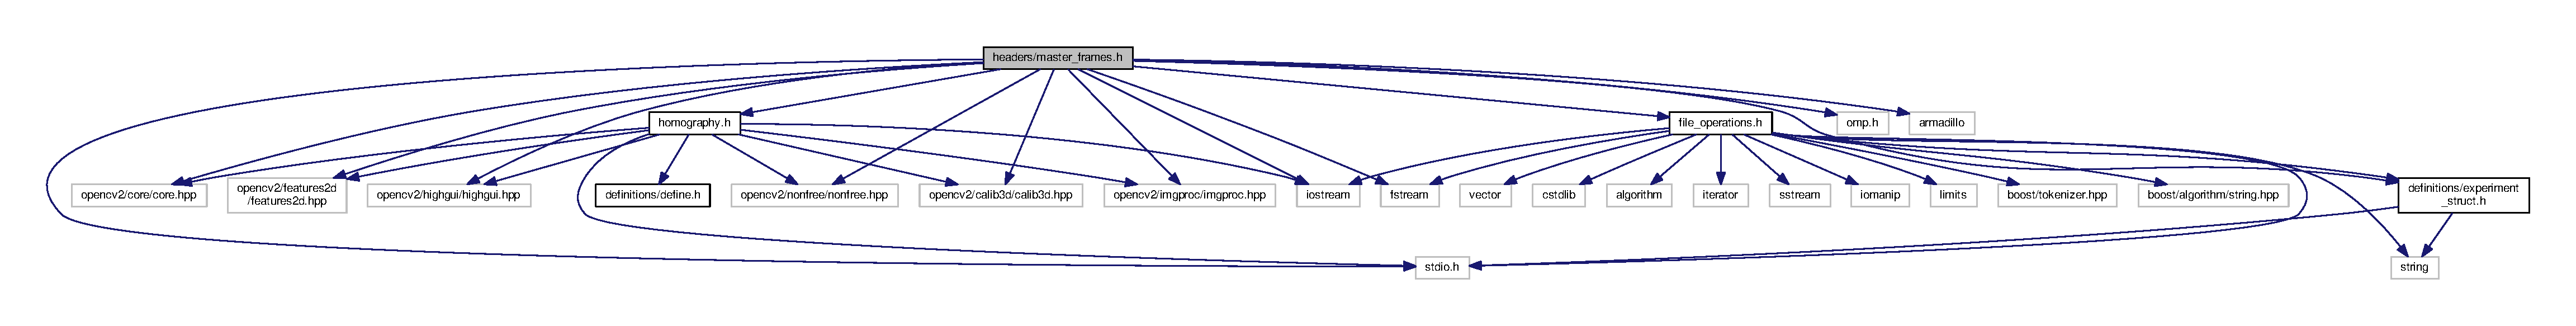
\includegraphics[width=350pt]{master__frames_8h__incl}
\end{center}
\end{figure}
This graph shows which files directly or indirectly include this file\+:\nopagebreak
\begin{figure}[H]
\begin{center}
\leavevmode
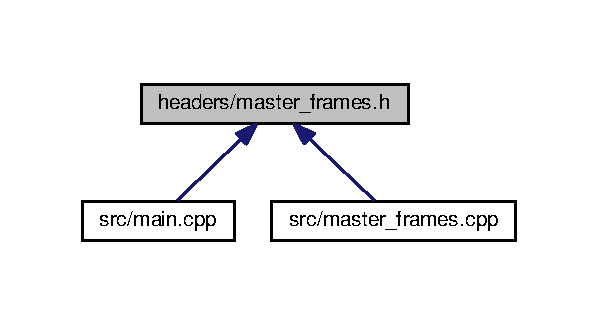
\includegraphics[width=287pt]{master__frames_8h__dep__incl}
\end{center}
\end{figure}
\subsection*{Functions}
\begin{DoxyCompactItemize}
\item 
std\+::vector$<$ int $>$ \hyperlink{master__frames_8h_af399de8fc7e31d60cccdf90efa80541c}{get\+Master\+Frames} (const \hyperlink{structEXPERIMENT}{E\+X\+P\+E\+R\+I\+M\+E\+NT} \hyperlink{main_8cpp_a9f5a81402e170475690f371d55cbe623}{experiment\+\_\+settings}, const int num\+\_\+frames)
\begin{DoxyCompactList}\small\item\em Function that return the master frames in a sequence according with experiment settings, by load from a file or calculating them. \end{DoxyCompactList}\item 
int \hyperlink{master__frames_8h_add63ac6145fd4d298e34df91185136b1}{length} (int number)
\begin{DoxyCompactList}\small\item\em Function that counts the digits of the number. \end{DoxyCompactList}\end{DoxyCompactItemize}


\subsection{Detailed Description}
Header functions for the \hyperlink{master__frames_8cpp}{master\+\_\+frames.\+cpp}. 



\subsection{Function Documentation}
\index{master\+\_\+frames.\+h@{master\+\_\+frames.\+h}!get\+Master\+Frames@{get\+Master\+Frames}}
\index{get\+Master\+Frames@{get\+Master\+Frames}!master\+\_\+frames.\+h@{master\+\_\+frames.\+h}}
\subsubsection[{\texorpdfstring{get\+Master\+Frames(const E\+X\+P\+E\+R\+I\+M\+E\+N\+T experiment\+\_\+settings, const int num\+\_\+frames)}{getMasterFrames(const EXPERIMENT experiment\_settings, const int num\_frames)}}]{\setlength{\rightskip}{0pt plus 5cm}std\+::vector$<$int$>$ get\+Master\+Frames (
\begin{DoxyParamCaption}
\item[{const {\bf E\+X\+P\+E\+R\+I\+M\+E\+NT}}]{experiment\+\_\+settings, }
\item[{const int}]{num\+\_\+frames}
\end{DoxyParamCaption}
)}\hypertarget{master__frames_8h_af399de8fc7e31d60cccdf90efa80541c}{}\label{master__frames_8h_af399de8fc7e31d60cccdf90efa80541c}


Function that return the master frames in a sequence according with experiment settings, by load from a file or calculating them. 


\begin{DoxyParams}{Parameters}
{\em experiment\+\_\+settings} & -\/ object with the experiment settings. \\
\hline
{\em num\+\_\+frames} & -\/ number of frames of the reduced video.\\
\hline
\end{DoxyParams}
\begin{DoxyReturn}{Returns}
{\ttfamily std\+::vector$<$int$>$} -\/ vector with the master frames found in the sequence.
\end{DoxyReturn}
\begin{DoxyAuthor}{Author}
Michel Melo da Silva 
\end{DoxyAuthor}
\begin{DoxyDate}{Date}
04/04/2016 
\end{DoxyDate}
\index{master\+\_\+frames.\+h@{master\+\_\+frames.\+h}!length@{length}}
\index{length@{length}!master\+\_\+frames.\+h@{master\+\_\+frames.\+h}}
\subsubsection[{\texorpdfstring{length(int number)}{length(int number)}}]{\setlength{\rightskip}{0pt plus 5cm}int length (
\begin{DoxyParamCaption}
\item[{int}]{number}
\end{DoxyParamCaption}
)}\hypertarget{master__frames_8h_add63ac6145fd4d298e34df91185136b1}{}\label{master__frames_8h_add63ac6145fd4d298e34df91185136b1}


Function that counts the digits of the number. 


\begin{DoxyParams}{Parameters}
{\em number} & -\/ number to calculate the number of digits.\\
\hline
\end{DoxyParams}
\begin{DoxyReturn}{Returns}
{\ttfamily int} -\/ number of digits of the input number.
\end{DoxyReturn}
\begin{DoxyAuthor}{Author}
Michel Melo da Silva 
\end{DoxyAuthor}
\begin{DoxyDate}{Date}
20/04/2016 
\end{DoxyDate}

\hypertarget{message__handler_8h}{}\section{headers/message\+\_\+handler.h File Reference}
\label{message__handler_8h}\index{headers/message\+\_\+handler.\+h@{headers/message\+\_\+handler.\+h}}
{\ttfamily \#include $<$stdio.\+h$>$}\\*
{\ttfamily \#include $<$iostream$>$}\\*
{\ttfamily \#include $<$fstream$>$}\\*
{\ttfamily \#include \char`\"{}headers/error\+\_\+messages.\+h\char`\"{}}\\*
Include dependency graph for message\+\_\+handler.\+h\+:\nopagebreak
\begin{figure}[H]
\begin{center}
\leavevmode
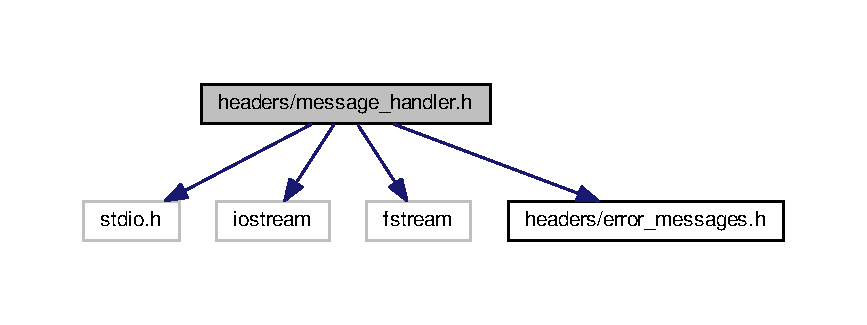
\includegraphics[width=350pt]{message__handler_8h__incl}
\end{center}
\end{figure}
This graph shows which files directly or indirectly include this file\+:\nopagebreak
\begin{figure}[H]
\begin{center}
\leavevmode
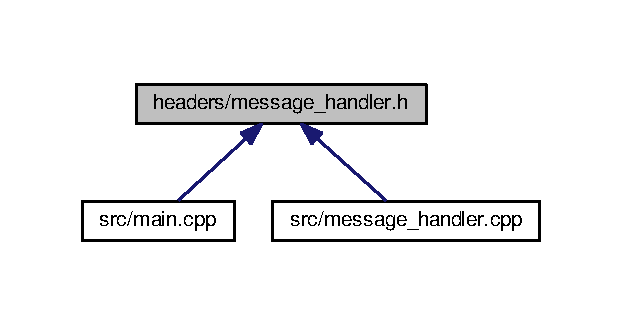
\includegraphics[width=299pt]{message__handler_8h__dep__incl}
\end{center}
\end{figure}
\subsection*{Classes}
\begin{DoxyCompactItemize}
\item 
class \hyperlink{classMessageHandler}{Message\+Handler}
\end{DoxyCompactItemize}
\subsection*{Enumerations}
\begin{DoxyCompactItemize}
\item 
enum \hyperlink{message__handler_8h_a0b8b584f5fb32277059bc4e6b9bcd6f0}{Stream} \{ \hyperlink{message__handler_8h_a0b8b584f5fb32277059bc4e6b9bcd6f0a05a425919d86aebc82762bd79990df56}{L\+O\+G\+\_\+\+F\+I\+LE}, 
\hyperlink{message__handler_8h_a0b8b584f5fb32277059bc4e6b9bcd6f0af2a9da294a4a62d55f04725d7efbb6ac}{S\+C\+R\+E\+EN}, 
\hyperlink{message__handler_8h_a0b8b584f5fb32277059bc4e6b9bcd6f0a627abe5a430420baf29ebe1940a7f2fb}{B\+O\+TH}
 \}
\end{DoxyCompactItemize}


\subsection{Enumeration Type Documentation}
\index{message\+\_\+handler.\+h@{message\+\_\+handler.\+h}!Stream@{Stream}}
\index{Stream@{Stream}!message\+\_\+handler.\+h@{message\+\_\+handler.\+h}}
\subsubsection[{\texorpdfstring{Stream}{Stream}}]{\setlength{\rightskip}{0pt plus 5cm}enum {\bf Stream}}\hypertarget{message__handler_8h_a0b8b584f5fb32277059bc4e6b9bcd6f0}{}\label{message__handler_8h_a0b8b584f5fb32277059bc4e6b9bcd6f0}
\begin{Desc}
\item[Enumerator]\par
\begin{description}
\index{L\+O\+G\+\_\+\+F\+I\+LE@{L\+O\+G\+\_\+\+F\+I\+LE}!message\+\_\+handler.\+h@{message\+\_\+handler.\+h}}\index{message\+\_\+handler.\+h@{message\+\_\+handler.\+h}!L\+O\+G\+\_\+\+F\+I\+LE@{L\+O\+G\+\_\+\+F\+I\+LE}}\item[{\em 
L\+O\+G\+\_\+\+F\+I\+LE\hypertarget{message__handler_8h_a0b8b584f5fb32277059bc4e6b9bcd6f0a05a425919d86aebc82762bd79990df56}{}\label{message__handler_8h_a0b8b584f5fb32277059bc4e6b9bcd6f0a05a425919d86aebc82762bd79990df56}
}]\index{S\+C\+R\+E\+EN@{S\+C\+R\+E\+EN}!message\+\_\+handler.\+h@{message\+\_\+handler.\+h}}\index{message\+\_\+handler.\+h@{message\+\_\+handler.\+h}!S\+C\+R\+E\+EN@{S\+C\+R\+E\+EN}}\item[{\em 
S\+C\+R\+E\+EN\hypertarget{message__handler_8h_a0b8b584f5fb32277059bc4e6b9bcd6f0af2a9da294a4a62d55f04725d7efbb6ac}{}\label{message__handler_8h_a0b8b584f5fb32277059bc4e6b9bcd6f0af2a9da294a4a62d55f04725d7efbb6ac}
}]\index{B\+O\+TH@{B\+O\+TH}!message\+\_\+handler.\+h@{message\+\_\+handler.\+h}}\index{message\+\_\+handler.\+h@{message\+\_\+handler.\+h}!B\+O\+TH@{B\+O\+TH}}\item[{\em 
B\+O\+TH\hypertarget{message__handler_8h_a0b8b584f5fb32277059bc4e6b9bcd6f0a627abe5a430420baf29ebe1940a7f2fb}{}\label{message__handler_8h_a0b8b584f5fb32277059bc4e6b9bcd6f0a627abe5a430420baf29ebe1940a7f2fb}
}]\end{description}
\end{Desc}

\hypertarget{sequence__processing_8h}{}\section{headers/sequence\+\_\+processing.h File Reference}
\label{sequence__processing_8h}\index{headers/sequence\+\_\+processing.\+h@{headers/sequence\+\_\+processing.\+h}}


Header functions for the \hyperlink{sequence__processing_8cpp}{sequence\+\_\+processing.\+cpp}.  


{\ttfamily \#include $<$stdio.\+h$>$}\\*
{\ttfamily \#include $<$iostream$>$}\\*
{\ttfamily \#include $<$fstream$>$}\\*
{\ttfamily \#include $<$omp.\+h$>$}\\*
{\ttfamily \#include $<$armadillo$>$}\\*
{\ttfamily \#include $<$opencv2/core/core.\+hpp$>$}\\*
{\ttfamily \#include $<$opencv2/features2d/features2d.\+hpp$>$}\\*
{\ttfamily \#include $<$opencv2/highgui/highgui.\+hpp$>$}\\*
{\ttfamily \#include $<$opencv2/nonfree/nonfree.\+hpp$>$}\\*
{\ttfamily \#include $<$opencv2/calib3d/calib3d.\+hpp$>$}\\*
{\ttfamily \#include $<$opencv2/imgproc/imgproc.\+hpp$>$}\\*
{\ttfamily \#include \char`\"{}definitions/experiment\+\_\+struct.\+h\char`\"{}}\\*
{\ttfamily \#include \char`\"{}file\+\_\+operations.\+h\char`\"{}}\\*
Include dependency graph for sequence\+\_\+processing.\+h\+:\nopagebreak
\begin{figure}[H]
\begin{center}
\leavevmode
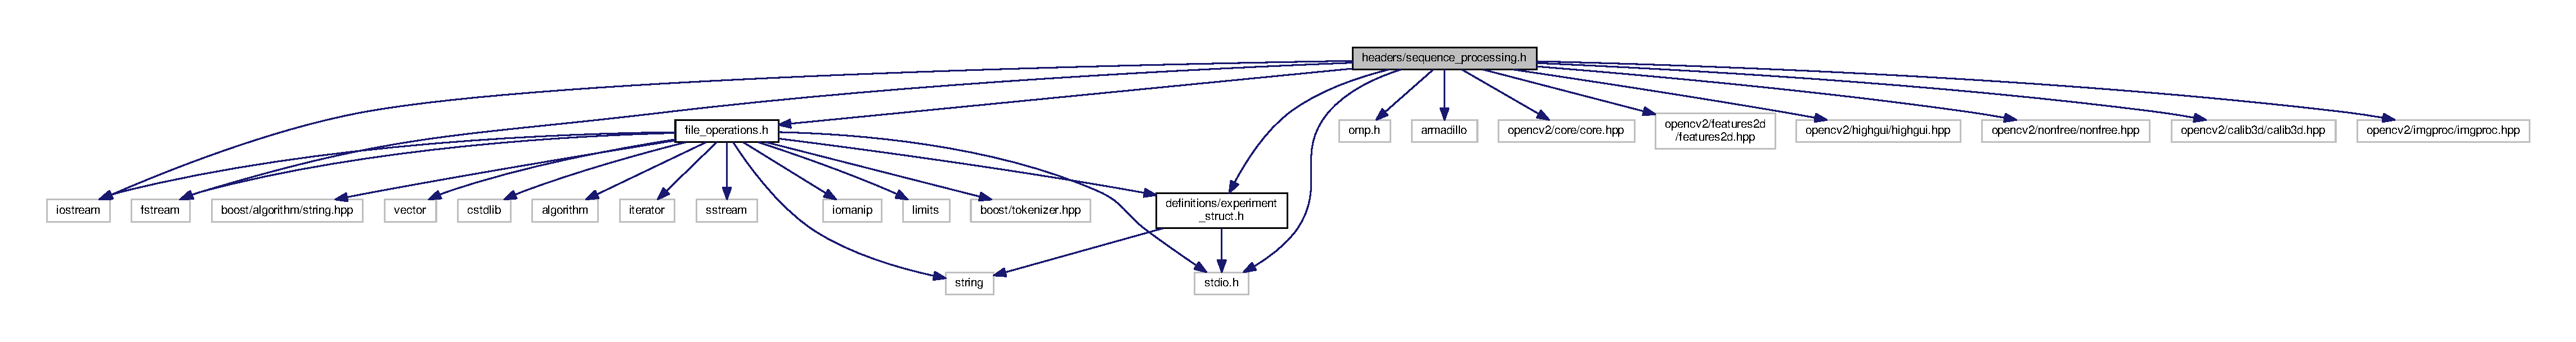
\includegraphics[width=350pt]{sequence__processing_8h__incl}
\end{center}
\end{figure}
This graph shows which files directly or indirectly include this file\+:\nopagebreak
\begin{figure}[H]
\begin{center}
\leavevmode
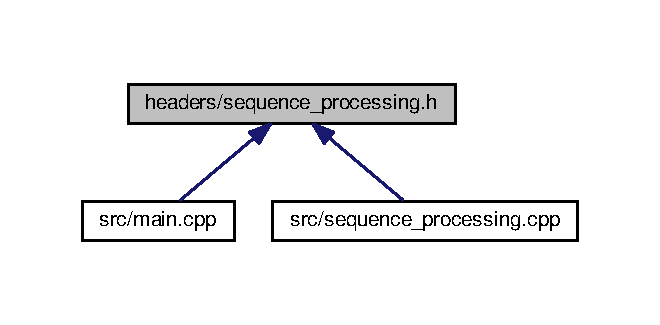
\includegraphics[width=317pt]{sequence__processing_8h__dep__incl}
\end{center}
\end{figure}
\subsection*{Functions}
\begin{DoxyCompactItemize}
\item 
bool \hyperlink{sequence__processing_8h_aad08ac53f56a97ead9e9e2a4e167e4d8}{find\+Intermediate\+Homography\+Matrix} (const int d, const int D, const int N, const cv\+::\+Mat \&frame\+\_\+i, const cv\+::\+Mat \&frame\+\_\+master\+\_\+pre, const cv\+::\+Mat \&frame\+\_\+master\+\_\+pos, cv\+::\+Mat \&homography\+\_\+matrix\+\_\+result)
\begin{DoxyCompactList}\small\item\em Function that calculates the homography matrix that leave the frame\+\_\+i to the intermediate plan between the plans of frame\+\_\+master\+\_\+pre and frame\+\_\+master\+\_\+pre with relation of the distance between them. \end{DoxyCompactList}\item 
bool \hyperlink{sequence__processing_8h_a536d6b62274f62941d6cec32549d2543}{find\+Intermediate\+Homography\+Matrix} (const int d, const int D, const int N, const cv\+::\+Mat \&frame\+\_\+i, const std\+::vector$<$ cv\+::\+Key\+Point $>$ \&keypoints\+\_\+master\+\_\+pre, const std\+::vector$<$ cv\+::\+Key\+Point $>$ \&keypoints\+\_\+master\+\_\+pos, const cv\+::\+Mat \&descriptors\+\_\+master\+\_\+pre, const cv\+::\+Mat \&descriptors\+\_\+master\+\_\+pos, cv\+::\+Mat \&homography\+\_\+matrix\+\_\+result)
\begin{DoxyCompactList}\small\item\em Function that calculates the homography matrix that leave the frame\+\_\+i to the intermediate plan between the frames related to the previous and posterior master, with respect to the distance between them. \end{DoxyCompactList}\item 
bool \hyperlink{sequence__processing_8h_aa692e8a44dcab5dc3c45c35c3f7ae6d2}{find\+Intermediate\+Homography\+Matrix} (const float s, const float S, const cv\+::\+Mat \&frame\+\_\+i, const std\+::vector$<$ cv\+::\+Key\+Point $>$ \&keypoints\+\_\+master\+\_\+pre, const std\+::vector$<$ cv\+::\+Key\+Point $>$ \&keypoints\+\_\+master\+\_\+pos, const cv\+::\+Mat \&descriptors\+\_\+master\+\_\+pre, const cv\+::\+Mat \&descriptors\+\_\+master\+\_\+pos, cv\+::\+Mat \&homography\+\_\+matrix\+\_\+result)
\begin{DoxyCompactList}\small\item\em Function that calculates the homography matrix that leave the frame\+\_\+i to the intermediate plan between the frames related to the previous and posterior master, with respect to the distance between them. \end{DoxyCompactList}\item 
int \hyperlink{sequence__processing_8h_a8374c98e95b78cc5027c494103e35348}{select\+New\+Frame} (const int d, const int D, const int N, const int index, const int index\+\_\+previous, const int index\+\_\+posterior, const std\+::vector$<$ cv\+::\+Key\+Point $>$ \&keypoints\+\_\+master\+\_\+pre, const std\+::vector$<$ cv\+::\+Key\+Point $>$ \&keypoints\+\_\+master\+\_\+pos, const cv\+::\+Mat \&descriptors\+\_\+master\+\_\+pre, const cv\+::\+Mat \&descriptors\+\_\+master\+\_\+pos, const cv\+::\+Rect \&crop\+\_\+area, const \hyperlink{structEXPERIMENT}{E\+X\+P\+E\+R\+I\+M\+E\+NT} \&\hyperlink{main_8cpp_a9f5a81402e170475690f371d55cbe623}{experiment\+\_\+settings}, cv\+::\+Mat \&new\+\_\+frame)
\begin{DoxyCompactList}\small\item\em Function that selects a new frame in the original video using the values of semantic information of the transition from the frame\+\_\+src to the frame\+\_\+dst calculted by M\+A\+T\+L\+AB and saved in a C\+SV file, the area ratio of the iamge after apply the homography transformation and the R\+A\+N\+S\+C\+AC inliers from the previous and posterior frames that compose the reduced video. \end{DoxyCompactList}\item 
int \hyperlink{sequence__processing_8h_a029dc4caa330843be4ee108a5e7bb825}{select\+New\+Frame} (const float s, const float S, const int index, const int index\+\_\+previous, const int index\+\_\+posterior, const std\+::vector$<$ cv\+::\+Key\+Point $>$ \&keypoints\+\_\+master\+\_\+pre, const std\+::vector$<$ cv\+::\+Key\+Point $>$ \&keypoints\+\_\+master\+\_\+pos, const cv\+::\+Mat \&descriptors\+\_\+master\+\_\+pre, const cv\+::\+Mat \&descriptors\+\_\+master\+\_\+pos, const cv\+::\+Rect \&crop\+\_\+area, const \hyperlink{structEXPERIMENT}{E\+X\+P\+E\+R\+I\+M\+E\+NT} \&\hyperlink{main_8cpp_a9f5a81402e170475690f371d55cbe623}{experiment\+\_\+settings}, cv\+::\+Mat \&new\+\_\+frame)
\begin{DoxyCompactList}\small\item\em Function that selects a new frame in the original video using the values of semantic information of the transition from the frame\+\_\+src to the frame\+\_\+dst calculted by M\+A\+T\+L\+AB and saved in a C\+SV file, the area ratio of the iamge after apply the homography transformation and the R\+A\+N\+S\+C\+AC inliers from the previous and posterior frames that compose the reduced video. \end{DoxyCompactList}\end{DoxyCompactItemize}


\subsection{Detailed Description}
Header functions for the \hyperlink{sequence__processing_8cpp}{sequence\+\_\+processing.\+cpp}. 



\subsection{Function Documentation}
\index{sequence\+\_\+processing.\+h@{sequence\+\_\+processing.\+h}!find\+Intermediate\+Homography\+Matrix@{find\+Intermediate\+Homography\+Matrix}}
\index{find\+Intermediate\+Homography\+Matrix@{find\+Intermediate\+Homography\+Matrix}!sequence\+\_\+processing.\+h@{sequence\+\_\+processing.\+h}}
\subsubsection[{\texorpdfstring{find\+Intermediate\+Homography\+Matrix(const int d, const int D, const int N, const cv\+::\+Mat \&frame\+\_\+i, const cv\+::\+Mat \&frame\+\_\+master\+\_\+pre, const cv\+::\+Mat \&frame\+\_\+master\+\_\+pos, cv\+::\+Mat \&homography\+\_\+matrix\+\_\+result)}{findIntermediateHomographyMatrix(const int d, const int D, const int N, const cv::Mat \&frame\_i, const cv::Mat \&frame\_master\_pre, const cv::Mat \&frame\_master\_pos, cv::Mat \&homography\_matrix\_result)}}]{\setlength{\rightskip}{0pt plus 5cm}bool find\+Intermediate\+Homography\+Matrix (
\begin{DoxyParamCaption}
\item[{const int}]{d, }
\item[{const int}]{D, }
\item[{const int}]{N, }
\item[{const cv\+::\+Mat \&}]{frame\+\_\+i, }
\item[{const cv\+::\+Mat \&}]{frame\+\_\+master\+\_\+pre, }
\item[{const cv\+::\+Mat \&}]{frame\+\_\+master\+\_\+pos, }
\item[{cv\+::\+Mat \&}]{homography\+\_\+matrix\+\_\+result}
\end{DoxyParamCaption}
)}\hypertarget{sequence__processing_8h_aad08ac53f56a97ead9e9e2a4e167e4d8}{}\label{sequence__processing_8h_aad08ac53f56a97ead9e9e2a4e167e4d8}


Function that calculates the homography matrix that leave the frame\+\_\+i to the intermediate plan between the plans of frame\+\_\+master\+\_\+pre and frame\+\_\+master\+\_\+pre with relation of the distance between them. 


\begin{DoxyParams}{Parameters}
{\em d} & -\/ distance between the current frame and the previous master frame. \\
\hline
{\em D} & -\/ distance between previous master frame and the posterior master frame. \\
\hline
{\em N} & -\/ size of the segments. \\
\hline
{\em frame\+\_\+i} & -\/ current image. \\
\hline
{\em frame\+\_\+master\+\_\+pre} & -\/ image of the previous master frame. \\
\hline
{\em frame\+\_\+master\+\_\+pos} & -\/ image of the posterior master frame. \\
\hline
{\em homography\+\_\+matrix\+\_\+result} & -\/ object to save the result homography matrix.\\
\hline
\end{DoxyParams}
\begin{DoxyReturn}{Returns}
{\ttfamily bool} {\bfseries true} -\/ if there is enough points in both images and good matches between them to find a homography matrix. ~\newline
 {\ttfamily bool} {\ttfamily false} -\/ if there is not enough points in both images or good matches between them to find a homography matrix.
\end{DoxyReturn}
\begin{DoxyAuthor}{Author}
Michel Melo da Silva 
\end{DoxyAuthor}
\begin{DoxyDate}{Date}
04/04/2016
\end{DoxyDate}

\begin{DoxyParams}{Parameters}
{\em d} & -\/ distance between the current frame and the previous master frame. \\
\hline
{\em D} & -\/ distance between previous master frame and the posterior master frame. \\
\hline
{\em N} & -\/ size of the segments. \\
\hline
{\em frame\+\_\+i} & -\/ current frame. \\
\hline
{\em frame\+\_\+master\+\_\+pre} & -\/ image of the previous master frame. \\
\hline
{\em frame\+\_\+master\+\_\+pos} & -\/ image of the posterior master frame. \\
\hline
{\em homography\+\_\+matrix\+\_\+result} & -\/ object to save the result homography matrix.\\
\hline
\end{DoxyParams}
\begin{DoxyReturn}{Returns}
{\ttfamily bool} {\bfseries true} -\/ if there is enough points in both images and good matches between them to find a homography matrix. ~\newline
 {\ttfamily bool} {\ttfamily false} -\/ if there is not enough points in both images or good matches between them to find a homography matrix.
\end{DoxyReturn}
\begin{DoxyAuthor}{Author}
Michel Melo da Silva 
\end{DoxyAuthor}
\begin{DoxyDate}{Date}
04/04/2016 
\end{DoxyDate}
\index{sequence\+\_\+processing.\+h@{sequence\+\_\+processing.\+h}!find\+Intermediate\+Homography\+Matrix@{find\+Intermediate\+Homography\+Matrix}}
\index{find\+Intermediate\+Homography\+Matrix@{find\+Intermediate\+Homography\+Matrix}!sequence\+\_\+processing.\+h@{sequence\+\_\+processing.\+h}}
\subsubsection[{\texorpdfstring{find\+Intermediate\+Homography\+Matrix(const int d, const int D, const int N, const cv\+::\+Mat \&frame\+\_\+i, const std\+::vector$<$ cv\+::\+Key\+Point $>$ \&keypoints\+\_\+master\+\_\+pre, const std\+::vector$<$ cv\+::\+Key\+Point $>$ \&keypoints\+\_\+master\+\_\+pos, const cv\+::\+Mat \&descriptors\+\_\+master\+\_\+pre, const cv\+::\+Mat \&descriptors\+\_\+master\+\_\+pos, cv\+::\+Mat \&homography\+\_\+matrix\+\_\+result)}{findIntermediateHomographyMatrix(const int d, const int D, const int N, const cv::Mat \&frame\_i, const std::vector< cv::KeyPoint > \&keypoints\_master\_pre, const std::vector< cv::KeyPoint > \&keypoints\_master\_pos, const cv::Mat \&descriptors\_master\_pre, const cv::Mat \&descriptors\_master\_pos, cv::Mat \&homography\_matrix\_result)}}]{\setlength{\rightskip}{0pt plus 5cm}bool find\+Intermediate\+Homography\+Matrix (
\begin{DoxyParamCaption}
\item[{const int}]{d, }
\item[{const int}]{D, }
\item[{const int}]{N, }
\item[{const cv\+::\+Mat \&}]{frame\+\_\+i, }
\item[{const std\+::vector$<$ cv\+::\+Key\+Point $>$ \&}]{keypoints\+\_\+master\+\_\+pre, }
\item[{const std\+::vector$<$ cv\+::\+Key\+Point $>$ \&}]{keypoints\+\_\+master\+\_\+pos, }
\item[{const cv\+::\+Mat \&}]{descriptors\+\_\+master\+\_\+pre, }
\item[{const cv\+::\+Mat \&}]{descriptors\+\_\+master\+\_\+pos, }
\item[{cv\+::\+Mat \&}]{homography\+\_\+matrix\+\_\+result}
\end{DoxyParamCaption}
)}\hypertarget{sequence__processing_8h_a536d6b62274f62941d6cec32549d2543}{}\label{sequence__processing_8h_a536d6b62274f62941d6cec32549d2543}


Function that calculates the homography matrix that leave the frame\+\_\+i to the intermediate plan between the frames related to the previous and posterior master, with respect to the distance between them. 


\begin{DoxyParams}{Parameters}
{\em d} & -\/ distance between the current frame and the previous master frame. \\
\hline
{\em D} & -\/ distance between previous master frame and the posterior master frame. \\
\hline
{\em N} & -\/ size of the segments. \\
\hline
{\em frame\+\_\+i} & -\/ current frame. \\
\hline
{\em keypoints\+\_\+master\+\_\+pre} & -\/ keypoints of the previous master. \\
\hline
{\em keypoints\+\_\+master\+\_\+pos} & -\/ keypoints of the posterior master. \\
\hline
{\em descriptors\+\_\+master\+\_\+pre} & -\/ descriptors of the previous master. \\
\hline
{\em descriptors\+\_\+master\+\_\+pos} & -\/ descriptors of the posterior master. \\
\hline
{\em homography\+\_\+matrix\+\_\+result} & -\/ object to save the result homography matrix.\\
\hline
\end{DoxyParams}
\begin{DoxyReturn}{Returns}
{\ttfamily bool} {\bfseries true} -\/ if there is enough points in both images and good matches between them to find a homography matrix. ~\newline
 {\ttfamily bool} {\ttfamily false} -\/ if there is not enough points in both images or good matches between them to find a homography matrix.
\end{DoxyReturn}
\begin{DoxyAuthor}{Author}
Washington Luis de Souza Ramos 
\end{DoxyAuthor}
\begin{DoxyDate}{Date}
30/08/2016 
\end{DoxyDate}
\index{sequence\+\_\+processing.\+h@{sequence\+\_\+processing.\+h}!find\+Intermediate\+Homography\+Matrix@{find\+Intermediate\+Homography\+Matrix}}
\index{find\+Intermediate\+Homography\+Matrix@{find\+Intermediate\+Homography\+Matrix}!sequence\+\_\+processing.\+h@{sequence\+\_\+processing.\+h}}
\subsubsection[{\texorpdfstring{find\+Intermediate\+Homography\+Matrix(const float s, const float S, const cv\+::\+Mat \&frame\+\_\+i, const std\+::vector$<$ cv\+::\+Key\+Point $>$ \&keypoints\+\_\+master\+\_\+pre, const std\+::vector$<$ cv\+::\+Key\+Point $>$ \&keypoints\+\_\+master\+\_\+pos, const cv\+::\+Mat \&descriptors\+\_\+master\+\_\+pre, const cv\+::\+Mat \&descriptors\+\_\+master\+\_\+pos, cv\+::\+Mat \&homography\+\_\+matrix\+\_\+result)}{findIntermediateHomographyMatrix(const float s, const float S, const cv::Mat \&frame\_i, const std::vector< cv::KeyPoint > \&keypoints\_master\_pre, const std::vector< cv::KeyPoint > \&keypoints\_master\_pos, const cv::Mat \&descriptors\_master\_pre, const cv::Mat \&descriptors\_master\_pos, cv::Mat \&homography\_matrix\_result)}}]{\setlength{\rightskip}{0pt plus 5cm}bool find\+Intermediate\+Homography\+Matrix (
\begin{DoxyParamCaption}
\item[{const float}]{s, }
\item[{const float}]{S, }
\item[{const cv\+::\+Mat \&}]{frame\+\_\+i, }
\item[{const std\+::vector$<$ cv\+::\+Key\+Point $>$ \&}]{keypoints\+\_\+master\+\_\+pre, }
\item[{const std\+::vector$<$ cv\+::\+Key\+Point $>$ \&}]{keypoints\+\_\+master\+\_\+pos, }
\item[{const cv\+::\+Mat \&}]{descriptors\+\_\+master\+\_\+pre, }
\item[{const cv\+::\+Mat \&}]{descriptors\+\_\+master\+\_\+pos, }
\item[{cv\+::\+Mat \&}]{homography\+\_\+matrix\+\_\+result}
\end{DoxyParamCaption}
)}\hypertarget{sequence__processing_8h_aa692e8a44dcab5dc3c45c35c3f7ae6d2}{}\label{sequence__processing_8h_aa692e8a44dcab5dc3c45c35c3f7ae6d2}


Function that calculates the homography matrix that leave the frame\+\_\+i to the intermediate plan between the frames related to the previous and posterior master, with respect to the distance between them. 


\begin{DoxyParams}{Parameters}
{\em d} & -\/ frame shift value between the previous master frame and the current frame. \\
\hline
{\em D} & -\/ frame shift between previous master frame and the posterior master frame. \\
\hline
{\em frame\+\_\+i} & -\/ current frame. \\
\hline
{\em keypoints\+\_\+master\+\_\+pre} & -\/ keypoints of the previous master. \\
\hline
{\em keypoints\+\_\+master\+\_\+pos} & -\/ keypoints of the posterior master. \\
\hline
{\em descriptors\+\_\+master\+\_\+pre} & -\/ descriptors of the previous master. \\
\hline
{\em descriptors\+\_\+master\+\_\+pos} & -\/ descriptors of the posterior master. \\
\hline
{\em homography\+\_\+matrix\+\_\+result} & -\/ object to save the result homography matrix.\\
\hline
\end{DoxyParams}
\begin{DoxyReturn}{Returns}
{\ttfamily bool} {\bfseries true} -\/ if there is enough points in both images and good matches between them to find a homography matrix. ~\newline
 {\ttfamily bool} {\ttfamily false} -\/ if there is not enough points in both images or good matches between them to find a homography matrix.
\end{DoxyReturn}
\begin{DoxyAuthor}{Author}
Washington Luis de Souza Ramos 
\end{DoxyAuthor}
\begin{DoxyDate}{Date}
08/09/2016
\end{DoxyDate}

\begin{DoxyParams}{Parameters}
{\em s} & -\/ frame shift value between the previous master frame and the current frame. \\
\hline
{\em S} & -\/ frame shift between previous master frame and the posterior master frame. \\
\hline
{\em frame\+\_\+i} & -\/ current frame. \\
\hline
{\em keypoints\+\_\+master\+\_\+pre} & -\/ keypoints of the previous master. \\
\hline
{\em keypoints\+\_\+master\+\_\+pos} & -\/ keypoints of the posterior master. \\
\hline
{\em descriptors\+\_\+master\+\_\+pre} & -\/ descriptors of the previous master. \\
\hline
{\em descriptors\+\_\+master\+\_\+pos} & -\/ descriptors of the posterior master. \\
\hline
{\em homography\+\_\+matrix\+\_\+result} & -\/ object to save the result homography matrix.\\
\hline
\end{DoxyParams}
\begin{DoxyReturn}{Returns}
{\ttfamily bool} {\bfseries true} -\/ if there is enough points in both images and good matches between them to find a homography matrix. ~\newline
 {\ttfamily bool} {\ttfamily false} -\/ if there is not enough points in both images or good matches between them to find a homography matrix.
\end{DoxyReturn}
\begin{DoxyAuthor}{Author}
Washington Luis de Souza Ramos 
\end{DoxyAuthor}
\begin{DoxyDate}{Date}
08/09/2016 
\end{DoxyDate}
\index{sequence\+\_\+processing.\+h@{sequence\+\_\+processing.\+h}!select\+New\+Frame@{select\+New\+Frame}}
\index{select\+New\+Frame@{select\+New\+Frame}!sequence\+\_\+processing.\+h@{sequence\+\_\+processing.\+h}}
\subsubsection[{\texorpdfstring{select\+New\+Frame(const int d, const int D, const int N, const int index, const int index\+\_\+previous, const int index\+\_\+posterior, const std\+::vector$<$ cv\+::\+Key\+Point $>$ \&keypoints\+\_\+master\+\_\+pre, const std\+::vector$<$ cv\+::\+Key\+Point $>$ \&keypoints\+\_\+master\+\_\+pos, const cv\+::\+Mat \&descriptors\+\_\+master\+\_\+pre, const cv\+::\+Mat \&descriptors\+\_\+master\+\_\+pos, const cv\+::\+Rect \&crop\+\_\+area, const E\+X\+P\+E\+R\+I\+M\+E\+N\+T \&experiment\+\_\+settings, cv\+::\+Mat \&new\+\_\+frame)}{selectNewFrame(const int d, const int D, const int N, const int index, const int index\_previous, const int index\_posterior, const std::vector< cv::KeyPoint > \&keypoints\_master\_pre, const std::vector< cv::KeyPoint > \&keypoints\_master\_pos, const cv::Mat \&descriptors\_master\_pre, const cv::Mat \&descriptors\_master\_pos, const cv::Rect \&crop\_area, const EXPERIMENT \&experiment\_settings, cv::Mat \&new\_frame)}}]{\setlength{\rightskip}{0pt plus 5cm}int select\+New\+Frame (
\begin{DoxyParamCaption}
\item[{const int}]{d, }
\item[{const int}]{D, }
\item[{const int}]{N, }
\item[{const int}]{index, }
\item[{const int}]{index\+\_\+previous, }
\item[{const int}]{index\+\_\+posterior, }
\item[{const std\+::vector$<$ cv\+::\+Key\+Point $>$ \&}]{keypoints\+\_\+master\+\_\+pre, }
\item[{const std\+::vector$<$ cv\+::\+Key\+Point $>$ \&}]{keypoints\+\_\+master\+\_\+pos, }
\item[{const cv\+::\+Mat \&}]{descriptors\+\_\+master\+\_\+pre, }
\item[{const cv\+::\+Mat \&}]{descriptors\+\_\+master\+\_\+pos, }
\item[{const cv\+::\+Rect \&}]{crop\+\_\+area, }
\item[{const {\bf E\+X\+P\+E\+R\+I\+M\+E\+NT} \&}]{experiment\+\_\+settings, }
\item[{cv\+::\+Mat \&}]{new\+\_\+frame}
\end{DoxyParamCaption}
)}\hypertarget{sequence__processing_8h_a8374c98e95b78cc5027c494103e35348}{}\label{sequence__processing_8h_a8374c98e95b78cc5027c494103e35348}


Function that selects a new frame in the original video using the values of semantic information of the transition from the frame\+\_\+src to the frame\+\_\+dst calculted by M\+A\+T\+L\+AB and saved in a C\+SV file, the area ratio of the iamge after apply the homography transformation and the R\+A\+N\+S\+C\+AC inliers from the previous and posterior frames that compose the reduced video. 


\begin{DoxyParams}{Parameters}
{\em d} & -\/ distance between the current frame and the previous master frame. \\
\hline
{\em D} & -\/ distance between previous master frame and the posterior master frame. \\
\hline
{\em N} & -\/ size of the segments. \\
\hline
{\em index} & -\/ index of the frame that will be replaced. \\
\hline
{\em index\+\_\+previous} & -\/ index of the last frame in the reduced video. \\
\hline
{\em index\+\_\+posterior} & -\/ index of the next frame in the reduced video. \\
\hline
{\em image\+\_\+master\+\_\+previous} & -\/ image with the master previous \\
\hline
{\em image\+\_\+master\+\_\+posterior} & -\/ image with the master posterior \\
\hline
{\em crop\+\_\+area} & -\/ crop area of the video. \\
\hline
{\em experiment\+\_\+settings} & -\/ experiment settings struct. \\
\hline
{\em new\+\_\+frame} & -\/ image that will receive the new selected frame.\\
\hline
\end{DoxyParams}
\begin{DoxyReturn}{Returns}
{\ttfamily int} -\/ returns the index of the new selected frame.
\end{DoxyReturn}
\begin{DoxyAuthor}{Author}
Michel Melo da Silva 
\end{DoxyAuthor}
\begin{DoxyDate}{Date}
30/04/2016 
\end{DoxyDate}
\index{sequence\+\_\+processing.\+h@{sequence\+\_\+processing.\+h}!select\+New\+Frame@{select\+New\+Frame}}
\index{select\+New\+Frame@{select\+New\+Frame}!sequence\+\_\+processing.\+h@{sequence\+\_\+processing.\+h}}
\subsubsection[{\texorpdfstring{select\+New\+Frame(const float s, const float S, const int index, const int index\+\_\+previous, const int index\+\_\+posterior, const std\+::vector$<$ cv\+::\+Key\+Point $>$ \&keypoints\+\_\+master\+\_\+pre, const std\+::vector$<$ cv\+::\+Key\+Point $>$ \&keypoints\+\_\+master\+\_\+pos, const cv\+::\+Mat \&descriptors\+\_\+master\+\_\+pre, const cv\+::\+Mat \&descriptors\+\_\+master\+\_\+pos, const cv\+::\+Rect \&crop\+\_\+area, const E\+X\+P\+E\+R\+I\+M\+E\+N\+T \&experiment\+\_\+settings, cv\+::\+Mat \&new\+\_\+frame)}{selectNewFrame(const float s, const float S, const int index, const int index\_previous, const int index\_posterior, const std::vector< cv::KeyPoint > \&keypoints\_master\_pre, const std::vector< cv::KeyPoint > \&keypoints\_master\_pos, const cv::Mat \&descriptors\_master\_pre, const cv::Mat \&descriptors\_master\_pos, const cv::Rect \&crop\_area, const EXPERIMENT \&experiment\_settings, cv::Mat \&new\_frame)}}]{\setlength{\rightskip}{0pt plus 5cm}int select\+New\+Frame (
\begin{DoxyParamCaption}
\item[{const float}]{s, }
\item[{const float}]{S, }
\item[{const int}]{index, }
\item[{const int}]{index\+\_\+previous, }
\item[{const int}]{index\+\_\+posterior, }
\item[{const std\+::vector$<$ cv\+::\+Key\+Point $>$ \&}]{keypoints\+\_\+master\+\_\+pre, }
\item[{const std\+::vector$<$ cv\+::\+Key\+Point $>$ \&}]{keypoints\+\_\+master\+\_\+pos, }
\item[{const cv\+::\+Mat \&}]{descriptors\+\_\+master\+\_\+pre, }
\item[{const cv\+::\+Mat \&}]{descriptors\+\_\+master\+\_\+pos, }
\item[{const cv\+::\+Rect \&}]{crop\+\_\+area, }
\item[{const {\bf E\+X\+P\+E\+R\+I\+M\+E\+NT} \&}]{experiment\+\_\+settings, }
\item[{cv\+::\+Mat \&}]{new\+\_\+frame}
\end{DoxyParamCaption}
)}\hypertarget{sequence__processing_8h_a029dc4caa330843be4ee108a5e7bb825}{}\label{sequence__processing_8h_a029dc4caa330843be4ee108a5e7bb825}


Function that selects a new frame in the original video using the values of semantic information of the transition from the frame\+\_\+src to the frame\+\_\+dst calculted by M\+A\+T\+L\+AB and saved in a C\+SV file, the area ratio of the iamge after apply the homography transformation and the R\+A\+N\+S\+C\+AC inliers from the previous and posterior frames that compose the reduced video. 


\begin{DoxyParams}{Parameters}
{\em s} & -\/ frame shift value between the previous master frame and the current frame. \\
\hline
{\em S} & -\/ frame shift between previous master frame and the posterior master frame. \\
\hline
{\em index} & -\/ index of the frame that will be replaced. \\
\hline
{\em index\+\_\+previous} & -\/ index of the last frame in the reduced video. \\
\hline
{\em index\+\_\+posterior} & -\/ index of the next frame in the reduced video. \\
\hline
{\em image\+\_\+master\+\_\+previous} & -\/ image with the master previous \\
\hline
{\em image\+\_\+master\+\_\+posterior} & -\/ image with the master posterior \\
\hline
{\em crop\+\_\+area} & -\/ crop area of the video. \\
\hline
{\em experiment\+\_\+settings} & -\/ experiment settings struct. \\
\hline
{\em new\+\_\+frame} & -\/ image that will receive the new selected frame.\\
\hline
\end{DoxyParams}
\begin{DoxyReturn}{Returns}
{\ttfamily int} -\/ returns the index of the new selected frame.
\end{DoxyReturn}
\begin{DoxyAuthor}{Author}
Washington Luis de Souza Ramos 
\end{DoxyAuthor}
\begin{DoxyDate}{Date}
08/09/2016 
\end{DoxyDate}

\hypertarget{README_8md}{}\section{R\+E\+A\+D\+M\+E.\+md File Reference}
\label{README_8md}\index{R\+E\+A\+D\+M\+E.\+md@{R\+E\+A\+D\+M\+E.\+md}}

\hypertarget{file__operations_8cpp}{}\section{src/file\+\_\+operations.cpp File Reference}
\label{file__operations_8cpp}\index{src/file\+\_\+operations.\+cpp@{src/file\+\_\+operations.\+cpp}}


Functions to manipulate files.  


{\ttfamily \#include \char`\"{}headers/file\+\_\+operations.\+h\char`\"{}}\\*
Include dependency graph for file\+\_\+operations.\+cpp\+:\nopagebreak
\begin{figure}[H]
\begin{center}
\leavevmode
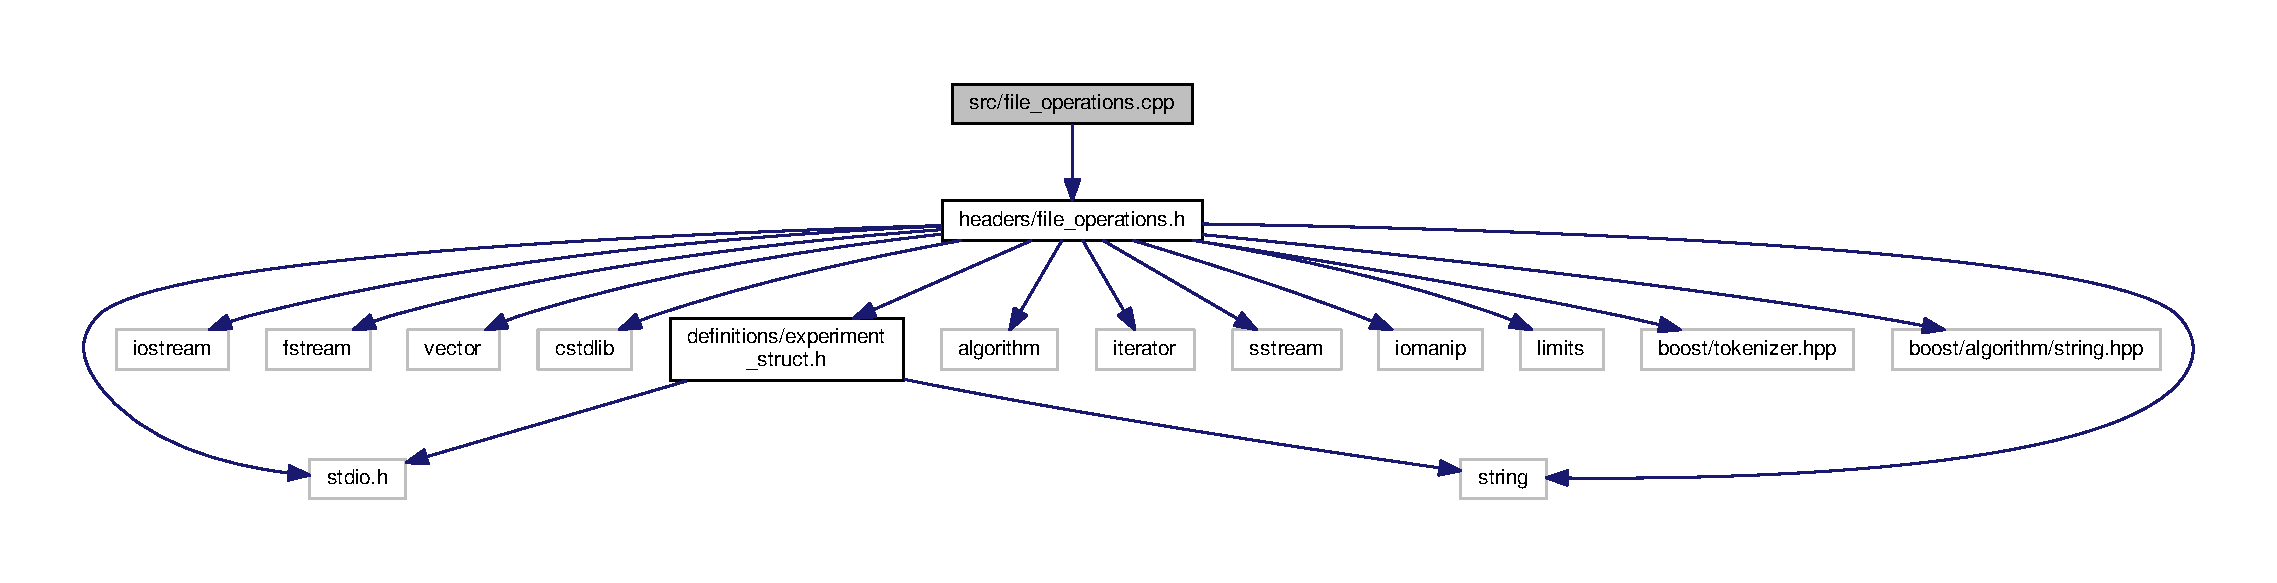
\includegraphics[width=350pt]{file__operations_8cpp__incl}
\end{center}
\end{figure}
\subsection*{Functions}
\begin{DoxyCompactItemize}
\item 
std\+::vector$<$ int $>$ \hyperlink{file__operations_8cpp_ad65b52efdd81718726a7c020b2745231}{load\+Master\+Frames\+From\+File} (const \hyperlink{structEXPERIMENT}{E\+X\+P\+E\+R\+I\+M\+E\+NT} \&\hyperlink{main_8cpp_a9f5a81402e170475690f371d55cbe623}{experiment\+\_\+settings})
\begin{DoxyCompactList}\small\item\em Function to load the master frames from a file defined in the field read\+\_\+masterframes\+\_\+filename in the experiment\+\_\+settings. \end{DoxyCompactList}\item 
bool \hyperlink{file__operations_8cpp_a8ee838aca4ec1d86b6da27d8d0c6c5a6}{save\+Master\+Frames\+To\+File} (const \hyperlink{structEXPERIMENT}{E\+X\+P\+E\+R\+I\+M\+E\+NT} \&\hyperlink{main_8cpp_a9f5a81402e170475690f371d55cbe623}{experiment\+\_\+settings}, const std\+::vector$<$ int $>$ masters\+\_\+frames)
\begin{DoxyCompactList}\small\item\em Function to save the calculated master frames into a file defined in the field save\+\_\+masterframes\+\_\+filename in the experiment\+\_\+settings. \end{DoxyCompactList}\item 
void \hyperlink{file__operations_8cpp_a65c5cb4d2def7f9475ee950799649709}{read\+Selected\+Frames\+C\+SV} (std\+::string filename, std\+::vector$<$ int $>$ \&selected\+\_\+frames)
\begin{DoxyCompactList}\small\item\em Function to read a C\+SV composed by frames selected by the selection algorithm. \end{DoxyCompactList}\item 
std\+::string \hyperlink{file__operations_8cpp_add54304682603740491ac7f2fa3e8909}{get\+Experiment\+Id} ()
\begin{DoxyCompactList}\small\item\em Function that manages the experiments ID automatically. \end{DoxyCompactList}\item 
std\+::istream \& \hyperlink{file__operations_8cpp_a67b6429613828d45a354bdbe54c98492}{go\+To\+Line} (std\+::istream \&file, const unsigned int line)
\begin{DoxyCompactList}\small\item\em Function that set the file pointer to the desired line, if it is smaller than the file number of lines. \end{DoxyCompactList}\item 
double \hyperlink{file__operations_8cpp_a4389609d14f1f46754e68ced749e4736}{get\+Semantic\+Cost} (const \hyperlink{structEXPERIMENT}{E\+X\+P\+E\+R\+I\+M\+E\+NT} \&\hyperlink{main_8cpp_a9f5a81402e170475690f371d55cbe623}{experiment\+\_\+settings}, const int frame\+\_\+src, const int frame\+\_\+dst)
\begin{DoxyCompactList}\small\item\em Function that returns the semantic cost of the transition from the frame\+\_\+src to the frame\+\_\+dst. \end{DoxyCompactList}\item 
std\+::vector$<$ std\+::vector$<$ double $>$ $>$ \hyperlink{file__operations_8cpp_a2995a8f3930a0b01a4e0ac1bfc5638e3}{load\+Instability\+Costs\+From\+File} (const \hyperlink{structEXPERIMENT}{E\+X\+P\+E\+R\+I\+M\+E\+NT} \&\hyperlink{main_8cpp_a9f5a81402e170475690f371d55cbe623}{experiment\+\_\+settings})
\begin{DoxyCompactList}\small\item\em load\+Instability\+Costs\+From\+File Loads the instability costs from a C\+SV file (matrix format). \end{DoxyCompactList}\item 
std\+::vector$<$ std\+::vector$<$ double $>$ $>$ \hyperlink{file__operations_8cpp_af95138c7e9d6611e1ace10ec85b633eb}{load\+Optical\+Flow} (const \hyperlink{structEXPERIMENT}{E\+X\+P\+E\+R\+I\+M\+E\+NT} \&\hyperlink{main_8cpp_a9f5a81402e170475690f371d55cbe623}{experiment\+\_\+settings})
\begin{DoxyCompactList}\small\item\em load\+Optical\+Flow Loads the Optical Flow calculated by the Flow\+Net from a C\+SV file. \end{DoxyCompactList}\item 
bool \hyperlink{file__operations_8cpp_a1e52e743807e450c3bdc8d8a179093ce}{str2bool} (std\+::string str)
\begin{DoxyCompactList}\small\item\em str2bool convert a string to boolean. \end{DoxyCompactList}\item 
std\+::string \hyperlink{file__operations_8cpp_a6fee1fe59a7b7ffbfff04e8e9b9e6571}{filter\+\_\+string} (std\+::string str)
\begin{DoxyCompactList}\small\item\em filter\+\_\+string filter a string to remove white spaces and line break. \end{DoxyCompactList}\end{DoxyCompactItemize}


\subsection{Detailed Description}
Functions to manipulate files. 

Functions to read from T\+XT and C\+SV files, write data on files. 

\subsection{Function Documentation}
\index{file\+\_\+operations.\+cpp@{file\+\_\+operations.\+cpp}!filter\+\_\+string@{filter\+\_\+string}}
\index{filter\+\_\+string@{filter\+\_\+string}!file\+\_\+operations.\+cpp@{file\+\_\+operations.\+cpp}}
\subsubsection[{\texorpdfstring{filter\+\_\+string(std\+::string str)}{filter\_string(std::string str)}}]{\setlength{\rightskip}{0pt plus 5cm}std\+::string filter\+\_\+string (
\begin{DoxyParamCaption}
\item[{std\+::string}]{str}
\end{DoxyParamCaption}
)}\hypertarget{file__operations_8cpp_a6fee1fe59a7b7ffbfff04e8e9b9e6571}{}\label{file__operations_8cpp_a6fee1fe59a7b7ffbfff04e8e9b9e6571}


filter\+\_\+string filter a string to remove white spaces and line break. 


\begin{DoxyParams}{Parameters}
{\em string} & \\
\hline
\end{DoxyParams}
\begin{DoxyReturn}{Returns}
string
\end{DoxyReturn}
\begin{DoxyAuthor}{Author}
Felipe Cadar Chamone 
\end{DoxyAuthor}
\begin{DoxyDate}{Date}
14/07/2017 
\end{DoxyDate}
\index{file\+\_\+operations.\+cpp@{file\+\_\+operations.\+cpp}!get\+Experiment\+Id@{get\+Experiment\+Id}}
\index{get\+Experiment\+Id@{get\+Experiment\+Id}!file\+\_\+operations.\+cpp@{file\+\_\+operations.\+cpp}}
\subsubsection[{\texorpdfstring{get\+Experiment\+Id()}{getExperimentId()}}]{\setlength{\rightskip}{0pt plus 5cm}std\+::string get\+Experiment\+Id (
\begin{DoxyParamCaption}
{}
\end{DoxyParamCaption}
)}\hypertarget{file__operations_8cpp_add54304682603740491ac7f2fa3e8909}{}\label{file__operations_8cpp_add54304682603740491ac7f2fa3e8909}


Function that manages the experiments ID automatically. 

\begin{DoxyReturn}{Returns}
{\ttfamily std\+::string} -\/ The experiment id formatted by 4 digits
\end{DoxyReturn}
\begin{DoxyAuthor}{Author}
Washington Luis de Souza Ramos 
\end{DoxyAuthor}
\begin{DoxyDate}{Date}
19/04/2016 
\end{DoxyDate}
\index{file\+\_\+operations.\+cpp@{file\+\_\+operations.\+cpp}!get\+Semantic\+Cost@{get\+Semantic\+Cost}}
\index{get\+Semantic\+Cost@{get\+Semantic\+Cost}!file\+\_\+operations.\+cpp@{file\+\_\+operations.\+cpp}}
\subsubsection[{\texorpdfstring{get\+Semantic\+Cost(const E\+X\+P\+E\+R\+I\+M\+E\+N\+T \&experiment\+\_\+settings, const int frame\+\_\+src, const int frame\+\_\+dst)}{getSemanticCost(const EXPERIMENT \&experiment\_settings, const int frame\_src, const int frame\_dst)}}]{\setlength{\rightskip}{0pt plus 5cm}double get\+Semantic\+Cost (
\begin{DoxyParamCaption}
\item[{const {\bf E\+X\+P\+E\+R\+I\+M\+E\+NT} \&}]{experiment\+\_\+settings, }
\item[{const int}]{frame\+\_\+src, }
\item[{const int}]{frame\+\_\+dst}
\end{DoxyParamCaption}
)}\hypertarget{file__operations_8cpp_a4389609d14f1f46754e68ced749e4736}{}\label{file__operations_8cpp_a4389609d14f1f46754e68ced749e4736}


Function that returns the semantic cost of the transition from the frame\+\_\+src to the frame\+\_\+dst. 

Function that returns the semantic cost of the transiction from the frame\+\_\+src to the frame\+\_\+dst.

The file where the semantic cost will be find is defined in the experiment\+\_\+settings


\begin{DoxyParams}{Parameters}
{\em experiment\+\_\+settings} & -\/ variable with the experiment setting. \\
\hline
{\em frame\+\_\+src} & -\/ first frame of the transition. \\
\hline
{\em frame\+\_\+dst} & -\/ last frame of the transition.\\
\hline
\end{DoxyParams}
\begin{DoxyReturn}{Returns}
{\ttfamily double} -\/ The semantic cost of the transiction of the frame\+\_\+src to the frame\+\_\+dst. Returns the complementary value ( 1 -\/ x ).
\end{DoxyReturn}
\begin{DoxyAuthor}{Author}
Michel Melo da Silva 
\end{DoxyAuthor}
\begin{DoxyDate}{Date}
30/04/2016 
\end{DoxyDate}
\index{file\+\_\+operations.\+cpp@{file\+\_\+operations.\+cpp}!go\+To\+Line@{go\+To\+Line}}
\index{go\+To\+Line@{go\+To\+Line}!file\+\_\+operations.\+cpp@{file\+\_\+operations.\+cpp}}
\subsubsection[{\texorpdfstring{go\+To\+Line(std\+::istream \&file, const unsigned int line)}{goToLine(std::istream \&file, const unsigned int line)}}]{\setlength{\rightskip}{0pt plus 5cm}std\+::istream\& go\+To\+Line (
\begin{DoxyParamCaption}
\item[{std\+::istream \&}]{file, }
\item[{const unsigned int}]{line}
\end{DoxyParamCaption}
)}\hypertarget{file__operations_8cpp_a67b6429613828d45a354bdbe54c98492}{}\label{file__operations_8cpp_a67b6429613828d45a354bdbe54c98492}


Function that set the file pointer to the desired line, if it is smaller than the file number of lines. 


\begin{DoxyParams}{Parameters}
{\em file} & -\/ std\+::ifstream object where the file is read. \\
\hline
{\em line} & -\/ line where the header read will be set.\\
\hline
\end{DoxyParams}
\begin{DoxyReturn}{Returns}
{\ttfamily std\+::istream} -\/ Reference to the file in the selected line.
\end{DoxyReturn}
\begin{DoxyAuthor}{Author}
Michel Melo da Silva 
\end{DoxyAuthor}
\begin{DoxyDate}{Date}
30/04/2016 
\end{DoxyDate}
\index{file\+\_\+operations.\+cpp@{file\+\_\+operations.\+cpp}!load\+Instability\+Costs\+From\+File@{load\+Instability\+Costs\+From\+File}}
\index{load\+Instability\+Costs\+From\+File@{load\+Instability\+Costs\+From\+File}!file\+\_\+operations.\+cpp@{file\+\_\+operations.\+cpp}}
\subsubsection[{\texorpdfstring{load\+Instability\+Costs\+From\+File(const E\+X\+P\+E\+R\+I\+M\+E\+N\+T \&experiment\+\_\+settings)}{loadInstabilityCostsFromFile(const EXPERIMENT \&experiment\_settings)}}]{\setlength{\rightskip}{0pt plus 5cm}std\+::vector$<$ std\+::vector$<$double$>$ $>$ load\+Instability\+Costs\+From\+File (
\begin{DoxyParamCaption}
\item[{const {\bf E\+X\+P\+E\+R\+I\+M\+E\+NT} \&}]{experiment\+\_\+settings}
\end{DoxyParamCaption}
)}\hypertarget{file__operations_8cpp_a2995a8f3930a0b01a4e0ac1bfc5638e3}{}\label{file__operations_8cpp_a2995a8f3930a0b01a4e0ac1bfc5638e3}


load\+Instability\+Costs\+From\+File Loads the instability costs from a C\+SV file (matrix format). 


\begin{DoxyParams}{Parameters}
{\em experiment\+\_\+settings} & \\
\hline
\end{DoxyParams}
\begin{DoxyReturn}{Returns}
The matrix of instability costs
\end{DoxyReturn}
\begin{DoxyAuthor}{Author}
Washington Luis de Souza Ramos 
\end{DoxyAuthor}
\begin{DoxyDate}{Date}
12/09/2016 
\end{DoxyDate}
\index{file\+\_\+operations.\+cpp@{file\+\_\+operations.\+cpp}!load\+Master\+Frames\+From\+File@{load\+Master\+Frames\+From\+File}}
\index{load\+Master\+Frames\+From\+File@{load\+Master\+Frames\+From\+File}!file\+\_\+operations.\+cpp@{file\+\_\+operations.\+cpp}}
\subsubsection[{\texorpdfstring{load\+Master\+Frames\+From\+File(const E\+X\+P\+E\+R\+I\+M\+E\+N\+T \&experiment\+\_\+settings)}{loadMasterFramesFromFile(const EXPERIMENT \&experiment\_settings)}}]{\setlength{\rightskip}{0pt plus 5cm}std\+::vector$<$int$>$ load\+Master\+Frames\+From\+File (
\begin{DoxyParamCaption}
\item[{const {\bf E\+X\+P\+E\+R\+I\+M\+E\+NT} \&}]{experiment\+\_\+settings}
\end{DoxyParamCaption}
)}\hypertarget{file__operations_8cpp_ad65b52efdd81718726a7c020b2745231}{}\label{file__operations_8cpp_ad65b52efdd81718726a7c020b2745231}


Function to load the master frames from a file defined in the field read\+\_\+masterframes\+\_\+filename in the experiment\+\_\+settings. 


\begin{DoxyParams}{Parameters}
{\em experiment\+\_\+settings} & -\/ variable with the experiment setting.\\
\hline
\end{DoxyParams}
\begin{DoxyReturn}{Returns}
{\ttfamily std\+::vector} -\/ vector of master frames loaded from file describle in the experiment settings.
\end{DoxyReturn}
\begin{DoxyAuthor}{Author}
Michel Melo da Silva 
\end{DoxyAuthor}
\begin{DoxyDate}{Date}
08/04/2016 
\end{DoxyDate}
\index{file\+\_\+operations.\+cpp@{file\+\_\+operations.\+cpp}!load\+Optical\+Flow@{load\+Optical\+Flow}}
\index{load\+Optical\+Flow@{load\+Optical\+Flow}!file\+\_\+operations.\+cpp@{file\+\_\+operations.\+cpp}}
\subsubsection[{\texorpdfstring{load\+Optical\+Flow(const E\+X\+P\+E\+R\+I\+M\+E\+N\+T \&experiment\+\_\+settings)}{loadOpticalFlow(const EXPERIMENT \&experiment\_settings)}}]{\setlength{\rightskip}{0pt plus 5cm}std\+::vector$<$ std\+::vector$<$double$>$ $>$ load\+Optical\+Flow (
\begin{DoxyParamCaption}
\item[{const {\bf E\+X\+P\+E\+R\+I\+M\+E\+NT} \&}]{experiment\+\_\+settings}
\end{DoxyParamCaption}
)}\hypertarget{file__operations_8cpp_af95138c7e9d6611e1ace10ec85b633eb}{}\label{file__operations_8cpp_af95138c7e9d6611e1ace10ec85b633eb}


load\+Optical\+Flow Loads the Optical Flow calculated by the Flow\+Net from a C\+SV file. 


\begin{DoxyParams}{Parameters}
{\em experiment\+\_\+settings} & \\
\hline
\end{DoxyParams}
\begin{DoxyReturn}{Returns}
Vector\mbox{[}j\mbox{]}\mbox{[}i\mbox{]} with the optical flow from the image j to j+1 (i=0 is dx and i=1 is dy).
\end{DoxyReturn}
\begin{DoxyAuthor}{Author}
Michel Melo da Silva 
\end{DoxyAuthor}
\begin{DoxyDate}{Date}
09/01/2017 
\end{DoxyDate}
\index{file\+\_\+operations.\+cpp@{file\+\_\+operations.\+cpp}!read\+Selected\+Frames\+C\+SV@{read\+Selected\+Frames\+C\+SV}}
\index{read\+Selected\+Frames\+C\+SV@{read\+Selected\+Frames\+C\+SV}!file\+\_\+operations.\+cpp@{file\+\_\+operations.\+cpp}}
\subsubsection[{\texorpdfstring{read\+Selected\+Frames\+C\+S\+V(std\+::string filename, std\+::vector$<$ int $>$ \&selected\+\_\+frames)}{readSelectedFramesCSV(std::string filename, std::vector< int > \&selected\_frames)}}]{\setlength{\rightskip}{0pt plus 5cm}void read\+Selected\+Frames\+C\+SV (
\begin{DoxyParamCaption}
\item[{std\+::string}]{filename, }
\item[{std\+::vector$<$ int $>$ \&}]{selected\+\_\+frames}
\end{DoxyParamCaption}
)}\hypertarget{file__operations_8cpp_a65c5cb4d2def7f9475ee950799649709}{}\label{file__operations_8cpp_a65c5cb4d2def7f9475ee950799649709}


Function to read a C\+SV composed by frames selected by the selection algorithm. 


\begin{DoxyParams}{Parameters}
{\em filename} & -\/ std\+::string with the filename of the C\+SV file that contains the selected frames of the reduced video. \\
\hline
{\em selected\+\_\+frames} & -\/ vector to save the selected frames.\\
\hline
\end{DoxyParams}
\begin{DoxyReturn}{Returns}
{\ttfamily void} 
\end{DoxyReturn}
\begin{DoxyAuthor}{Author}
Washington Luis de Souza Ramos 
\end{DoxyAuthor}
\begin{DoxyDate}{Date}
14/04/2016 
\end{DoxyDate}
\index{file\+\_\+operations.\+cpp@{file\+\_\+operations.\+cpp}!save\+Master\+Frames\+To\+File@{save\+Master\+Frames\+To\+File}}
\index{save\+Master\+Frames\+To\+File@{save\+Master\+Frames\+To\+File}!file\+\_\+operations.\+cpp@{file\+\_\+operations.\+cpp}}
\subsubsection[{\texorpdfstring{save\+Master\+Frames\+To\+File(const E\+X\+P\+E\+R\+I\+M\+E\+N\+T \&experiment\+\_\+settings, const std\+::vector$<$ int $>$ masters\+\_\+frames)}{saveMasterFramesToFile(const EXPERIMENT \&experiment\_settings, const std::vector< int > masters\_frames)}}]{\setlength{\rightskip}{0pt plus 5cm}bool save\+Master\+Frames\+To\+File (
\begin{DoxyParamCaption}
\item[{const {\bf E\+X\+P\+E\+R\+I\+M\+E\+NT} \&}]{experiment\+\_\+settings, }
\item[{const std\+::vector$<$ int $>$}]{masters\+\_\+frames}
\end{DoxyParamCaption}
)}\hypertarget{file__operations_8cpp_a8ee838aca4ec1d86b6da27d8d0c6c5a6}{}\label{file__operations_8cpp_a8ee838aca4ec1d86b6da27d8d0c6c5a6}


Function to save the calculated master frames into a file defined in the field save\+\_\+masterframes\+\_\+filename in the experiment\+\_\+settings. 


\begin{DoxyParams}{Parameters}
{\em experiment\+\_\+settings} & -\/ variable with the experiment setting. \\
\hline
{\em masters\+\_\+frames} & -\/ vector of master frames to be saved in file describle in the experiment settings.\\
\hline
\end{DoxyParams}
\begin{DoxyReturn}{Returns}
{\ttfamily bool} {\bfseries true} -\/ if the writer return sucess while writing the file. ~\newline
 {\ttfamily bool} {\bfseries false} -\/ if the writer return fail while writing the file.
\end{DoxyReturn}
\begin{DoxyAuthor}{Author}
Michel Melo da Silva 
\end{DoxyAuthor}
\begin{DoxyDate}{Date}
08/04/2016 
\end{DoxyDate}
\index{file\+\_\+operations.\+cpp@{file\+\_\+operations.\+cpp}!str2bool@{str2bool}}
\index{str2bool@{str2bool}!file\+\_\+operations.\+cpp@{file\+\_\+operations.\+cpp}}
\subsubsection[{\texorpdfstring{str2bool(std\+::string str)}{str2bool(std::string str)}}]{\setlength{\rightskip}{0pt plus 5cm}bool str2bool (
\begin{DoxyParamCaption}
\item[{std\+::string}]{str}
\end{DoxyParamCaption}
)}\hypertarget{file__operations_8cpp_a1e52e743807e450c3bdc8d8a179093ce}{}\label{file__operations_8cpp_a1e52e743807e450c3bdc8d8a179093ce}


str2bool convert a string to boolean. 


\begin{DoxyParams}{Parameters}
{\em string} & \\
\hline
\end{DoxyParams}
\begin{DoxyReturn}{Returns}
boolean
\end{DoxyReturn}
\begin{DoxyAuthor}{Author}
Felipe Cadar Chamone 
\end{DoxyAuthor}
\begin{DoxyDate}{Date}
14/07/2017 
\end{DoxyDate}

\hypertarget{homography_8cpp}{}\section{src/homography.cpp File Reference}
\label{homography_8cpp}\index{src/homography.\+cpp@{src/homography.\+cpp}}


Functions related with homography transformation.  


{\ttfamily \#include \char`\"{}definitions/define.\+h\char`\"{}}\\*
{\ttfamily \#include \char`\"{}headers/homography.\+h\char`\"{}}\\*
Include dependency graph for homography.\+cpp\+:\nopagebreak
\begin{figure}[H]
\begin{center}
\leavevmode
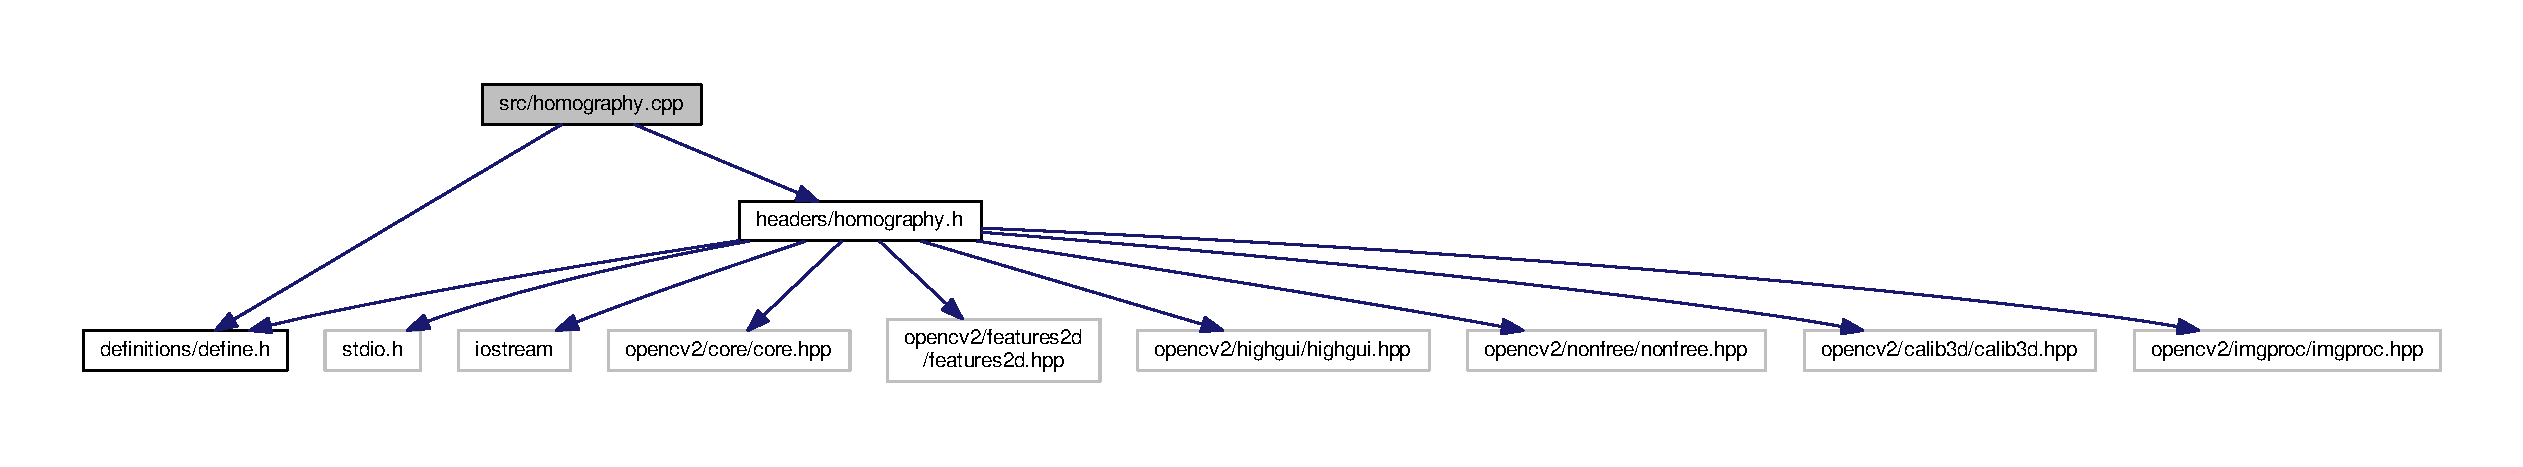
\includegraphics[width=350pt]{homography_8cpp__incl}
\end{center}
\end{figure}
\subsection*{Functions}
\begin{DoxyCompactItemize}
\item 
bool \hyperlink{homography_8cpp_a1d3798a81d0d3b5e8b24087a7bc60683}{find\+Homography\+Matrix} (const cv\+::\+Mat \&image\+\_\+src, const cv\+::\+Mat \&image\+\_\+dst, cv\+::\+Mat \&homography\+\_\+matrix, cv\+::\+Mat \&ransac\+\_\+mask)
\begin{DoxyCompactList}\small\item\em Function that find the homography matrix that leaves the image\+Src to the plan of the image\+Dst. \end{DoxyCompactList}\item 
bool \hyperlink{homography_8cpp_a1bf28b8d881beac4a6deee5cbe7ae4da}{find\+Homography\+Matrix} (const cv\+::\+Mat \&image\+\_\+src, const cv\+::\+Mat \&image\+\_\+dst, cv\+::\+Mat \&homography\+\_\+matrix)
\begin{DoxyCompactList}\small\item\em Function that find the homography matrix that leaves the image\+Src to the plan of the image\+Dst. \end{DoxyCompactList}\item 
bool \hyperlink{homography_8cpp_a3800765da624f694682f5f1fab7f4c63}{find\+Homography\+Matrix} (const std\+::vector$<$ cv\+::\+Key\+Point $>$ \&keypoints\+\_\+image\+\_\+src, const std\+::vector$<$ cv\+::\+Key\+Point $>$ \&keypoints\+\_\+image\+\_\+dst, const cv\+::\+Mat \&descriptors\+\_\+image\+\_\+src, const cv\+::\+Mat \&descriptors\+\_\+image\+\_\+dst, cv\+::\+Mat \&homography\+\_\+matrix, cv\+::\+Mat \&ransac\+\_\+mask)
\begin{DoxyCompactList}\small\item\em Function that finds the homography matrix given the keypoints and descriptors. \end{DoxyCompactList}\item 
bool \hyperlink{homography_8cpp_ae3833c553b4d2ea9817440dfc6f9b441}{find\+Homography\+Matrix} (const std\+::vector$<$ cv\+::\+Key\+Point $>$ \&keypoints\+\_\+image\+\_\+src, const std\+::vector$<$ cv\+::\+Key\+Point $>$ \&keypoints\+\_\+image\+\_\+dst, const cv\+::\+Mat \&descriptors\+\_\+image\+\_\+src, const cv\+::\+Mat \&descriptors\+\_\+image\+\_\+dst, cv\+::\+Mat \&homography\+\_\+matrix)
\begin{DoxyCompactList}\small\item\em Function that find the homography matrix that leaves the image\+Src to the plan of the image\+Dst. \end{DoxyCompactList}\item 
bool \hyperlink{homography_8cpp_af396adc4b5a19e8194e5ff96640f16de}{apply\+Homography\+Matrix} (const cv\+::\+Mat \&image\+\_\+src, const cv\+::\+Mat \&homography\+\_\+matrix, cv\+::\+Mat \&image\+\_\+result)
\begin{DoxyCompactList}\small\item\em Function that apply homography matrix in a given image. \end{DoxyCompactList}\item 
bool \hyperlink{homography_8cpp_a67a02c0cff3e126daece706c97c9ba2c}{check\+Homography\+Consistency} (const std\+::vector$<$ cv\+::\+Point2f $>$ img\+\_\+corners, const cv\+::\+Mat \&homography\+\_\+matrix)
\begin{DoxyCompactList}\small\item\em Function that checks if after made the homography transformation the corner consistency is maintained. \end{DoxyCompactList}\item 
bool \hyperlink{homography_8cpp_a3c17440ceb61568f04b508a4336c3402}{check\+Homography\+Consistency} (const std\+::vector$<$ cv\+::\+Point2f $>$ new\+\_\+img\+\_\+corners)
\begin{DoxyCompactList}\small\item\em Function that checks if after made the homography transformation the corner consistency is maintained. \end{DoxyCompactList}\item 
double \hyperlink{homography_8cpp_a94196b6d4321a287adf2b3051a5fad83}{get\+Area\+Ratio} (const cv\+::\+Mat \&image\+\_\+src, const cv\+::\+Mat \&homography\+\_\+matrix, const cv\+::\+Rect \&frame\+\_\+limits)
\begin{DoxyCompactList}\small\item\em Function that calculates the loss(\%) of the homography transformation in a R\+OI. \end{DoxyCompactList}\item 
\hyperlink{homography_8h_a340f89166e818e04b9c370262c161789}{Homog\+Coverage} \hyperlink{homography_8cpp_a8007547c4ef0394a46a61a21b6eab88c}{get\+Homog\+Coverage} (const cv\+::\+Mat \&image\+\_\+src, const cv\+::\+Mat \&homography\+\_\+matrix, const cv\+::\+Rect \&drop\+\_\+area, const cv\+::\+Rect \&crop\+\_\+area)
\begin{DoxyCompactList}\small\item\em Function that calculates the loss(\%) of the homography transformation in a R\+OI. \end{DoxyCompactList}\item 
void \hyperlink{homography_8cpp_af766393f5eb33e81f7f77f8ddc17cf03}{get\+Keypoints\+And\+Descriptors} (const cv\+::\+Mat \&image, std\+::vector$<$ cv\+::\+Key\+Point $>$ \&keypoints, cv\+::\+Mat \&descriptors)
\begin{DoxyCompactList}\small\item\em Function that gets the keypoints and describe an image in order to avoid unnecessary computations for tasks like finding the homography matrix. \end{DoxyCompactList}\end{DoxyCompactItemize}


\subsection{Detailed Description}
Functions related with homography transformation. 

Functions find homography matrix between two images. Apply homography matrix. Check if the image corner consistency is held after application of the homography matrix. Check the area ratio between the image after the homography matrix application and the frame boundaries. 

\subsection{Function Documentation}
\index{homography.\+cpp@{homography.\+cpp}!apply\+Homography\+Matrix@{apply\+Homography\+Matrix}}
\index{apply\+Homography\+Matrix@{apply\+Homography\+Matrix}!homography.\+cpp@{homography.\+cpp}}
\subsubsection[{\texorpdfstring{apply\+Homography\+Matrix(const cv\+::\+Mat \&image\+\_\+src, const cv\+::\+Mat \&homography\+\_\+matrix, cv\+::\+Mat \&image\+\_\+result)}{applyHomographyMatrix(const cv::Mat \&image\_src, const cv::Mat \&homography\_matrix, cv::Mat \&image\_result)}}]{\setlength{\rightskip}{0pt plus 5cm}bool apply\+Homography\+Matrix (
\begin{DoxyParamCaption}
\item[{const cv\+::\+Mat \&}]{image\+\_\+src, }
\item[{const cv\+::\+Mat \&}]{homography\+\_\+matrix, }
\item[{cv\+::\+Mat \&}]{image\+\_\+result}
\end{DoxyParamCaption}
)}\hypertarget{homography_8cpp_af396adc4b5a19e8194e5ff96640f16de}{}\label{homography_8cpp_af396adc4b5a19e8194e5ff96640f16de}


Function that apply homography matrix in a given image. 


\begin{DoxyParams}{Parameters}
{\em image\+\_\+src} & -\/ image where the homography matrix will be applied. \\
\hline
{\em homography\+\_\+matrix} & -\/ homography matrix. \\
\hline
{\em image\+\_\+result} & -\/ object to save the image after the application of the homography matrix.\\
\hline
\end{DoxyParams}
\begin{DoxyReturn}{Returns}
{\ttfamily bool} {\bfseries true} -\/ if the corner consistency is maintained after application of the homography matrix. ~\newline
 {\ttfamily bool} {\bfseries false} -\/ if the consistency is not maintained after application of the homography matrix. In this case the image\+Result is a simple copy of the image\+Src.
\end{DoxyReturn}
\begin{DoxyAuthor}{Author}
Michel Melo da Silva 
\end{DoxyAuthor}
\begin{DoxyDate}{Date}
25/03/2016 
\end{DoxyDate}
\index{homography.\+cpp@{homography.\+cpp}!check\+Homography\+Consistency@{check\+Homography\+Consistency}}
\index{check\+Homography\+Consistency@{check\+Homography\+Consistency}!homography.\+cpp@{homography.\+cpp}}
\subsubsection[{\texorpdfstring{check\+Homography\+Consistency(const std\+::vector$<$ cv\+::\+Point2f $>$ img\+\_\+corners, const cv\+::\+Mat \&homography\+\_\+matrix)}{checkHomographyConsistency(const std::vector< cv::Point2f > img\_corners, const cv::Mat \&homography\_matrix)}}]{\setlength{\rightskip}{0pt plus 5cm}bool check\+Homography\+Consistency (
\begin{DoxyParamCaption}
\item[{const std\+::vector$<$ cv\+::\+Point2f $>$}]{img\+\_\+corners, }
\item[{const cv\+::\+Mat \&}]{homography\+\_\+matrix}
\end{DoxyParamCaption}
)}\hypertarget{homography_8cpp_a67a02c0cff3e126daece706c97c9ba2c}{}\label{homography_8cpp_a67a02c0cff3e126daece706c97c9ba2c}


Function that checks if after made the homography transformation the corner consistency is maintained. 


\begin{DoxyParams}{Parameters}
{\em img\+\_\+corners} & -\/ image corners in the following order\+: ~\newline
 {\ttfamily img\+\_\+corners}\mbox{[}0\mbox{]} = 0 , 0 ~\newline
 {\ttfamily img\+\_\+corners}\mbox{[}1\mbox{]} = cols , 0 ~\newline
 {\ttfamily img\+\_\+corners}\mbox{[}2\mbox{]} = 0 , rows ~\newline
 {\ttfamily img\+\_\+corners}\mbox{[}3\mbox{]} = cols , rows \\
\hline
{\em homography\+\_\+matrix} & -\/ homography matrix that will be checked the consistency.\\
\hline
\end{DoxyParams}
\begin{DoxyReturn}{Returns}
{\ttfamily bool} {\bfseries true} -\/ if the consistency is maintained. ~\newline
 {\ttfamily bool} {\bfseries false} -\/ if the consistency is not maintained.
\end{DoxyReturn}
\begin{DoxyAuthor}{Author}
Michel Melo da Silva 
\end{DoxyAuthor}
\begin{DoxyDate}{Date}
08/04/2016 
\end{DoxyDate}
\index{homography.\+cpp@{homography.\+cpp}!check\+Homography\+Consistency@{check\+Homography\+Consistency}}
\index{check\+Homography\+Consistency@{check\+Homography\+Consistency}!homography.\+cpp@{homography.\+cpp}}
\subsubsection[{\texorpdfstring{check\+Homography\+Consistency(const std\+::vector$<$ cv\+::\+Point2f $>$ new\+\_\+img\+\_\+corners)}{checkHomographyConsistency(const std::vector< cv::Point2f > new\_img\_corners)}}]{\setlength{\rightskip}{0pt plus 5cm}bool check\+Homography\+Consistency (
\begin{DoxyParamCaption}
\item[{const std\+::vector$<$ cv\+::\+Point2f $>$}]{new\+\_\+img\+\_\+corners}
\end{DoxyParamCaption}
)}\hypertarget{homography_8cpp_a3c17440ceb61568f04b508a4336c3402}{}\label{homography_8cpp_a3c17440ceb61568f04b508a4336c3402}


Function that checks if after made the homography transformation the corner consistency is maintained. 


\begin{DoxyParams}{Parameters}
{\em new\+\_\+img\+\_\+corners} & -\/ image corners in the following order\+: ~\newline
 {\ttfamily img\+\_\+corners}\mbox{[}0\mbox{]} = 0 , 0 ~\newline
 {\ttfamily img\+\_\+corners}\mbox{[}1\mbox{]} = cols , 0 ~\newline
 {\ttfamily img\+\_\+corners}\mbox{[}2\mbox{]} = 0 , rows ~\newline
 {\ttfamily img\+\_\+corners}\mbox{[}3\mbox{]} = cols , rows\\
\hline
\end{DoxyParams}
\begin{DoxyReturn}{Returns}
{\ttfamily bool} {\bfseries true} -\/ if the consistency is maintained. ~\newline
 {\ttfamily bool} {\bfseries false} -\/ if the consistency is not maintained.
\end{DoxyReturn}
\begin{DoxyAuthor}{Author}
Michel Melo da Silva 
\end{DoxyAuthor}
\begin{DoxyDate}{Date}
12/04/2016 
\end{DoxyDate}
\index{homography.\+cpp@{homography.\+cpp}!find\+Homography\+Matrix@{find\+Homography\+Matrix}}
\index{find\+Homography\+Matrix@{find\+Homography\+Matrix}!homography.\+cpp@{homography.\+cpp}}
\subsubsection[{\texorpdfstring{find\+Homography\+Matrix(const cv\+::\+Mat \&image\+\_\+src, const cv\+::\+Mat \&image\+\_\+dst, cv\+::\+Mat \&homography\+\_\+matrix, cv\+::\+Mat \&ransac\+\_\+mask)}{findHomographyMatrix(const cv::Mat \&image\_src, const cv::Mat \&image\_dst, cv::Mat \&homography\_matrix, cv::Mat \&ransac\_mask)}}]{\setlength{\rightskip}{0pt plus 5cm}bool find\+Homography\+Matrix (
\begin{DoxyParamCaption}
\item[{const cv\+::\+Mat \&}]{image\+\_\+src, }
\item[{const cv\+::\+Mat \&}]{image\+\_\+dst, }
\item[{cv\+::\+Mat \&}]{homography\+\_\+matrix, }
\item[{cv\+::\+Mat \&}]{ransac\+\_\+mask}
\end{DoxyParamCaption}
)}\hypertarget{homography_8cpp_a1d3798a81d0d3b5e8b24087a7bc60683}{}\label{homography_8cpp_a1d3798a81d0d3b5e8b24087a7bc60683}


Function that find the homography matrix that leaves the image\+Src to the plan of the image\+Dst. 

Function that find the homography matrix that leave the image\+Src to the plan of the image\+Dst.

Returns the Ransak mask after finding the homography matrix.


\begin{DoxyParams}{Parameters}
{\em image\+\_\+src} & -\/ image to where the homography will be calculated. \\
\hline
{\em image\+\_\+dst} & -\/ image of the destination of the homography. \\
\hline
{\em homography\+\_\+matrix} & -\/ object to homography matrix calculated. \\
\hline
{\em ransac\+\_\+mask} & -\/ R\+A\+N\+S\+AC mask of the homography matrix. 1 means inliers and 0 means outliers.\\
\hline
\end{DoxyParams}
\begin{DoxyReturn}{Returns}
{\ttfamily bool} {\bfseries true} -\/ if there is enough points in both images and good matches between them to find a homography matrix. ~\newline
 {\ttfamily bool} {\bfseries false} -\/ if there is not enough points in both images or good matches between them to find a homography matrix.
\end{DoxyReturn}
\begin{DoxyAuthor}{Author}
Michel Melo da Silva 
\end{DoxyAuthor}
\begin{DoxyDate}{Date}
28/03/2016 
\end{DoxyDate}
\index{homography.\+cpp@{homography.\+cpp}!find\+Homography\+Matrix@{find\+Homography\+Matrix}}
\index{find\+Homography\+Matrix@{find\+Homography\+Matrix}!homography.\+cpp@{homography.\+cpp}}
\subsubsection[{\texorpdfstring{find\+Homography\+Matrix(const cv\+::\+Mat \&image\+\_\+src, const cv\+::\+Mat \&image\+\_\+dst, cv\+::\+Mat \&homography\+\_\+matrix)}{findHomographyMatrix(const cv::Mat \&image\_src, const cv::Mat \&image\_dst, cv::Mat \&homography\_matrix)}}]{\setlength{\rightskip}{0pt plus 5cm}bool find\+Homography\+Matrix (
\begin{DoxyParamCaption}
\item[{const cv\+::\+Mat \&}]{image\+\_\+src, }
\item[{const cv\+::\+Mat \&}]{image\+\_\+dst, }
\item[{cv\+::\+Mat \&}]{homography\+\_\+matrix}
\end{DoxyParamCaption}
)}\hypertarget{homography_8cpp_a1bf28b8d881beac4a6deee5cbe7ae4da}{}\label{homography_8cpp_a1bf28b8d881beac4a6deee5cbe7ae4da}


Function that find the homography matrix that leaves the image\+Src to the plan of the image\+Dst. 

Function that find the homography matrix that leave the image\+Src to the plan of the image\+Dst.


\begin{DoxyParams}{Parameters}
{\em image\+\_\+src} & -\/ image to where the homography will be calculated. \\
\hline
{\em image\+\_\+dst} & -\/ image of the destination of the homography. \\
\hline
{\em homography\+\_\+matrix} & -\/ object to save the homography matrix calculated.\\
\hline
\end{DoxyParams}
\begin{DoxyReturn}{Returns}
{\ttfamily bool} {\bfseries true} -\/ if there is enough points in both images and good matches between them to find a homography matrix. ~\newline
 {\ttfamily bool} {\bfseries false} -\/ if there is not enough points in both images or good matches between them to find a homography matrix.
\end{DoxyReturn}
\begin{DoxyAuthor}{Author}
Michel Melo da Silva 
\end{DoxyAuthor}
\begin{DoxyDate}{Date}
28/03/2016 
\end{DoxyDate}
\index{homography.\+cpp@{homography.\+cpp}!find\+Homography\+Matrix@{find\+Homography\+Matrix}}
\index{find\+Homography\+Matrix@{find\+Homography\+Matrix}!homography.\+cpp@{homography.\+cpp}}
\subsubsection[{\texorpdfstring{find\+Homography\+Matrix(const std\+::vector$<$ cv\+::\+Key\+Point $>$ \&keypoints\+\_\+image\+\_\+src, const std\+::vector$<$ cv\+::\+Key\+Point $>$ \&keypoints\+\_\+image\+\_\+dst, const cv\+::\+Mat \&descriptors\+\_\+image\+\_\+src, const cv\+::\+Mat \&descriptors\+\_\+image\+\_\+dst, cv\+::\+Mat \&homography\+\_\+matrix, cv\+::\+Mat \&ransac\+\_\+mask)}{findHomographyMatrix(const std::vector< cv::KeyPoint > \&keypoints\_image\_src, const std::vector< cv::KeyPoint > \&keypoints\_image\_dst, const cv::Mat \&descriptors\_image\_src, const cv::Mat \&descriptors\_image\_dst, cv::Mat \&homography\_matrix, cv::Mat \&ransac\_mask)}}]{\setlength{\rightskip}{0pt plus 5cm}bool find\+Homography\+Matrix (
\begin{DoxyParamCaption}
\item[{const std\+::vector$<$ cv\+::\+Key\+Point $>$ \&}]{keypoints\+\_\+image\+\_\+src, }
\item[{const std\+::vector$<$ cv\+::\+Key\+Point $>$ \&}]{keypoints\+\_\+image\+\_\+dst, }
\item[{const cv\+::\+Mat \&}]{descriptors\+\_\+image\+\_\+src, }
\item[{const cv\+::\+Mat \&}]{descriptors\+\_\+image\+\_\+dst, }
\item[{cv\+::\+Mat \&}]{homography\+\_\+matrix, }
\item[{cv\+::\+Mat \&}]{ransac\+\_\+mask}
\end{DoxyParamCaption}
)}\hypertarget{homography_8cpp_a3800765da624f694682f5f1fab7f4c63}{}\label{homography_8cpp_a3800765da624f694682f5f1fab7f4c63}


Function that finds the homography matrix given the keypoints and descriptors. 

Returns the Ransak mask after finding the homography matrix.


\begin{DoxyParams}{Parameters}
{\em keypoints\+\_\+image\+\_\+src} & -\/ keypoints of the source image. \\
\hline
{\em keypoints\+\_\+image\+\_\+dst} & -\/ keypoints of the target image. \\
\hline
{\em descriptors\+\_\+image\+\_\+src} & -\/ descriptors of the source image. \\
\hline
{\em descriptors\+\_\+image\+\_\+dst} & -\/ descriptors of the target image. \\
\hline
{\em homography\+\_\+matrix} & -\/ object to homography matrix calculated. \\
\hline
{\em ransac\+\_\+mask} & -\/ R\+A\+N\+S\+AC mask of the homography matrix. 1 means inliers and 0 means outliers.\\
\hline
\end{DoxyParams}
\begin{DoxyReturn}{Returns}
{\ttfamily bool} {\bfseries true} -\/ if there is enough points in both images and good matches between them to find a homography matrix. ~\newline
 {\ttfamily bool} {\bfseries false} -\/ if there is not enough points in both images or good matches between them to find a homography matrix.
\end{DoxyReturn}
\begin{DoxyAuthor}{Author}
Washington Luis de Souza Ramos 
\end{DoxyAuthor}
\begin{DoxyDate}{Date}
30/08/2016 
\end{DoxyDate}
\index{homography.\+cpp@{homography.\+cpp}!find\+Homography\+Matrix@{find\+Homography\+Matrix}}
\index{find\+Homography\+Matrix@{find\+Homography\+Matrix}!homography.\+cpp@{homography.\+cpp}}
\subsubsection[{\texorpdfstring{find\+Homography\+Matrix(const std\+::vector$<$ cv\+::\+Key\+Point $>$ \&keypoints\+\_\+image\+\_\+src, const std\+::vector$<$ cv\+::\+Key\+Point $>$ \&keypoints\+\_\+image\+\_\+dst, const cv\+::\+Mat \&descriptors\+\_\+image\+\_\+src, const cv\+::\+Mat \&descriptors\+\_\+image\+\_\+dst, cv\+::\+Mat \&homography\+\_\+matrix)}{findHomographyMatrix(const std::vector< cv::KeyPoint > \&keypoints\_image\_src, const std::vector< cv::KeyPoint > \&keypoints\_image\_dst, const cv::Mat \&descriptors\_image\_src, const cv::Mat \&descriptors\_image\_dst, cv::Mat \&homography\_matrix)}}]{\setlength{\rightskip}{0pt plus 5cm}bool find\+Homography\+Matrix (
\begin{DoxyParamCaption}
\item[{const std\+::vector$<$ cv\+::\+Key\+Point $>$ \&}]{keypoints\+\_\+image\+\_\+src, }
\item[{const std\+::vector$<$ cv\+::\+Key\+Point $>$ \&}]{keypoints\+\_\+image\+\_\+dst, }
\item[{const cv\+::\+Mat \&}]{descriptors\+\_\+image\+\_\+src, }
\item[{const cv\+::\+Mat \&}]{descriptors\+\_\+image\+\_\+dst, }
\item[{cv\+::\+Mat \&}]{homography\+\_\+matrix}
\end{DoxyParamCaption}
)}\hypertarget{homography_8cpp_ae3833c553b4d2ea9817440dfc6f9b441}{}\label{homography_8cpp_ae3833c553b4d2ea9817440dfc6f9b441}


Function that find the homography matrix that leaves the image\+Src to the plan of the image\+Dst. 


\begin{DoxyParams}{Parameters}
{\em keypoints\+\_\+image\+\_\+src} & -\/ keypoints of the source image. \\
\hline
{\em keypoints\+\_\+image\+\_\+dst} & -\/ keypoints of the target image. \\
\hline
{\em descriptors\+\_\+image\+\_\+src} & -\/ descriptors of the source image. \\
\hline
{\em descriptors\+\_\+image\+\_\+dst} & -\/ descriptors of the target image. \\
\hline
{\em homography\+\_\+matrix} & -\/ object to save the homography matrix calculated.\\
\hline
\end{DoxyParams}
\begin{DoxyReturn}{Returns}
{\ttfamily bool} {\bfseries true} -\/ if there is enough points in both images and good matches between them to find a homography matrix. ~\newline
 {\ttfamily bool} {\bfseries false} -\/ if there is not enough points in both images or good matches between them to find a homography matrix.
\end{DoxyReturn}
\begin{DoxyAuthor}{Author}
Washington Luis de Souza Ramos 
\end{DoxyAuthor}
\begin{DoxyDate}{Date}
09/09/2016 
\end{DoxyDate}
\index{homography.\+cpp@{homography.\+cpp}!get\+Area\+Ratio@{get\+Area\+Ratio}}
\index{get\+Area\+Ratio@{get\+Area\+Ratio}!homography.\+cpp@{homography.\+cpp}}
\subsubsection[{\texorpdfstring{get\+Area\+Ratio(const cv\+::\+Mat \&image\+\_\+src, const cv\+::\+Mat \&homography\+\_\+matrix, const cv\+::\+Rect \&frame\+\_\+limits)}{getAreaRatio(const cv::Mat \&image\_src, const cv::Mat \&homography\_matrix, const cv::Rect \&frame\_limits)}}]{\setlength{\rightskip}{0pt plus 5cm}double get\+Area\+Ratio (
\begin{DoxyParamCaption}
\item[{const cv\+::\+Mat \&}]{image\+\_\+src, }
\item[{const cv\+::\+Mat \&}]{homography\+\_\+matrix, }
\item[{const cv\+::\+Rect \&}]{frame\+\_\+limits}
\end{DoxyParamCaption}
)}\hypertarget{homography_8cpp_a94196b6d4321a287adf2b3051a5fad83}{}\label{homography_8cpp_a94196b6d4321a287adf2b3051a5fad83}


Function that calculates the loss(\%) of the homography transformation in a R\+OI. 

It returns the ratio between the non-\/image area and the frame\+\_\+limits area.


\begin{DoxyParams}{Parameters}
{\em image\+\_\+src} & -\/ The source image. \\
\hline
{\em homography\+\_\+matrix} & -\/ The homography matrix. \\
\hline
{\em frame\+\_\+limits} & -\/ The region of interest (R\+OI).\\
\hline
\end{DoxyParams}
\begin{DoxyReturn}{Returns}
{\ttfamily double} -\/ The ratio between non-\/image area and the whole frame area.
\end{DoxyReturn}
\begin{DoxyAuthor}{Author}
Washington Luis de Souza Ramos 
\end{DoxyAuthor}
\begin{DoxyDate}{Date}
14/04/2016 
\end{DoxyDate}
\index{homography.\+cpp@{homography.\+cpp}!get\+Homog\+Coverage@{get\+Homog\+Coverage}}
\index{get\+Homog\+Coverage@{get\+Homog\+Coverage}!homography.\+cpp@{homography.\+cpp}}
\subsubsection[{\texorpdfstring{get\+Homog\+Coverage(const cv\+::\+Mat \&image\+\_\+src, const cv\+::\+Mat \&homography\+\_\+matrix, const cv\+::\+Rect \&drop\+\_\+area, const cv\+::\+Rect \&crop\+\_\+area)}{getHomogCoverage(const cv::Mat \&image\_src, const cv::Mat \&homography\_matrix, const cv::Rect \&drop\_area, const cv::Rect \&crop\_area)}}]{\setlength{\rightskip}{0pt plus 5cm}{\bf Homog\+Coverage} get\+Homog\+Coverage (
\begin{DoxyParamCaption}
\item[{const cv\+::\+Mat \&}]{image\+\_\+src, }
\item[{const cv\+::\+Mat \&}]{homography\+\_\+matrix, }
\item[{const cv\+::\+Rect \&}]{drop\+\_\+area, }
\item[{const cv\+::\+Rect \&}]{crop\+\_\+area}
\end{DoxyParamCaption}
)}\hypertarget{homography_8cpp_a8007547c4ef0394a46a61a21b6eab88c}{}\label{homography_8cpp_a8007547c4ef0394a46a61a21b6eab88c}


Function that calculates the loss(\%) of the homography transformation in a R\+OI. 

It returns the coverage of a transformation which is N\+O\+NE, D\+R\+O\+P\+\_\+\+A\+R\+EA or C\+R\+O\+P\+\_\+\+A\+R\+EA. 
\begin{DoxyParams}{Parameters}
{\em image\+\_\+src} & -\/ The source image. \\
\hline
{\em homography\+\_\+matrix} & -\/ The homography matrix. \\
\hline
{\em drop\+\_\+area} & -\/ The region of interest (R\+OI) for the drop area. \\
\hline
{\em crop\+\_\+area} & -\/ The region of interest (R\+OI) for the crop area. \\
\hline
\end{DoxyParams}
\begin{DoxyReturn}{Returns}
The Homog\+Coverage enum value
\end{DoxyReturn}
\begin{DoxyAuthor}{Author}
Washington Luis de Souza Ramos 
\end{DoxyAuthor}
\begin{DoxyDate}{Date}
10/09/2016 
\end{DoxyDate}
\index{homography.\+cpp@{homography.\+cpp}!get\+Keypoints\+And\+Descriptors@{get\+Keypoints\+And\+Descriptors}}
\index{get\+Keypoints\+And\+Descriptors@{get\+Keypoints\+And\+Descriptors}!homography.\+cpp@{homography.\+cpp}}
\subsubsection[{\texorpdfstring{get\+Keypoints\+And\+Descriptors(const cv\+::\+Mat \&image, std\+::vector$<$ cv\+::\+Key\+Point $>$ \&keypoints, cv\+::\+Mat \&descriptors)}{getKeypointsAndDescriptors(const cv::Mat \&image, std::vector< cv::KeyPoint > \&keypoints, cv::Mat \&descriptors)}}]{\setlength{\rightskip}{0pt plus 5cm}void get\+Keypoints\+And\+Descriptors (
\begin{DoxyParamCaption}
\item[{const cv\+::\+Mat \&}]{image, }
\item[{std\+::vector$<$ cv\+::\+Key\+Point $>$ \&}]{keypoints, }
\item[{cv\+::\+Mat \&}]{descriptors}
\end{DoxyParamCaption}
)}\hypertarget{homography_8cpp_af766393f5eb33e81f7f77f8ddc17cf03}{}\label{homography_8cpp_af766393f5eb33e81f7f77f8ddc17cf03}


Function that gets the keypoints and describe an image in order to avoid unnecessary computations for tasks like finding the homography matrix. 


\begin{DoxyParams}{Parameters}
{\em image} & -\/ image to where the keypoints and descriptors are to be extracted from. \\
\hline
{\em keypoints} & -\/ the keypoints found in the image. \\
\hline
{\em descriptors} & -\/ the descriptors of the image.\\
\hline
\end{DoxyParams}
\begin{DoxyAuthor}{Author}
Washington Luis de Souza Ramos 
\end{DoxyAuthor}
\begin{DoxyDate}{Date}
30/08/2016 
\end{DoxyDate}

\hypertarget{image__reconstruction_8cpp}{}\section{src/image\+\_\+reconstruction.cpp File Reference}
\label{image__reconstruction_8cpp}\index{src/image\+\_\+reconstruction.\+cpp@{src/image\+\_\+reconstruction.\+cpp}}


Functions related with reconstruction of the image after application of the homography matrix to fill the whole frame boundaries.  


{\ttfamily \#include \char`\"{}headers/image\+\_\+reconstruction.\+h\char`\"{}}\\*
Include dependency graph for image\+\_\+reconstruction.\+cpp\+:\nopagebreak
\begin{figure}[H]
\begin{center}
\leavevmode
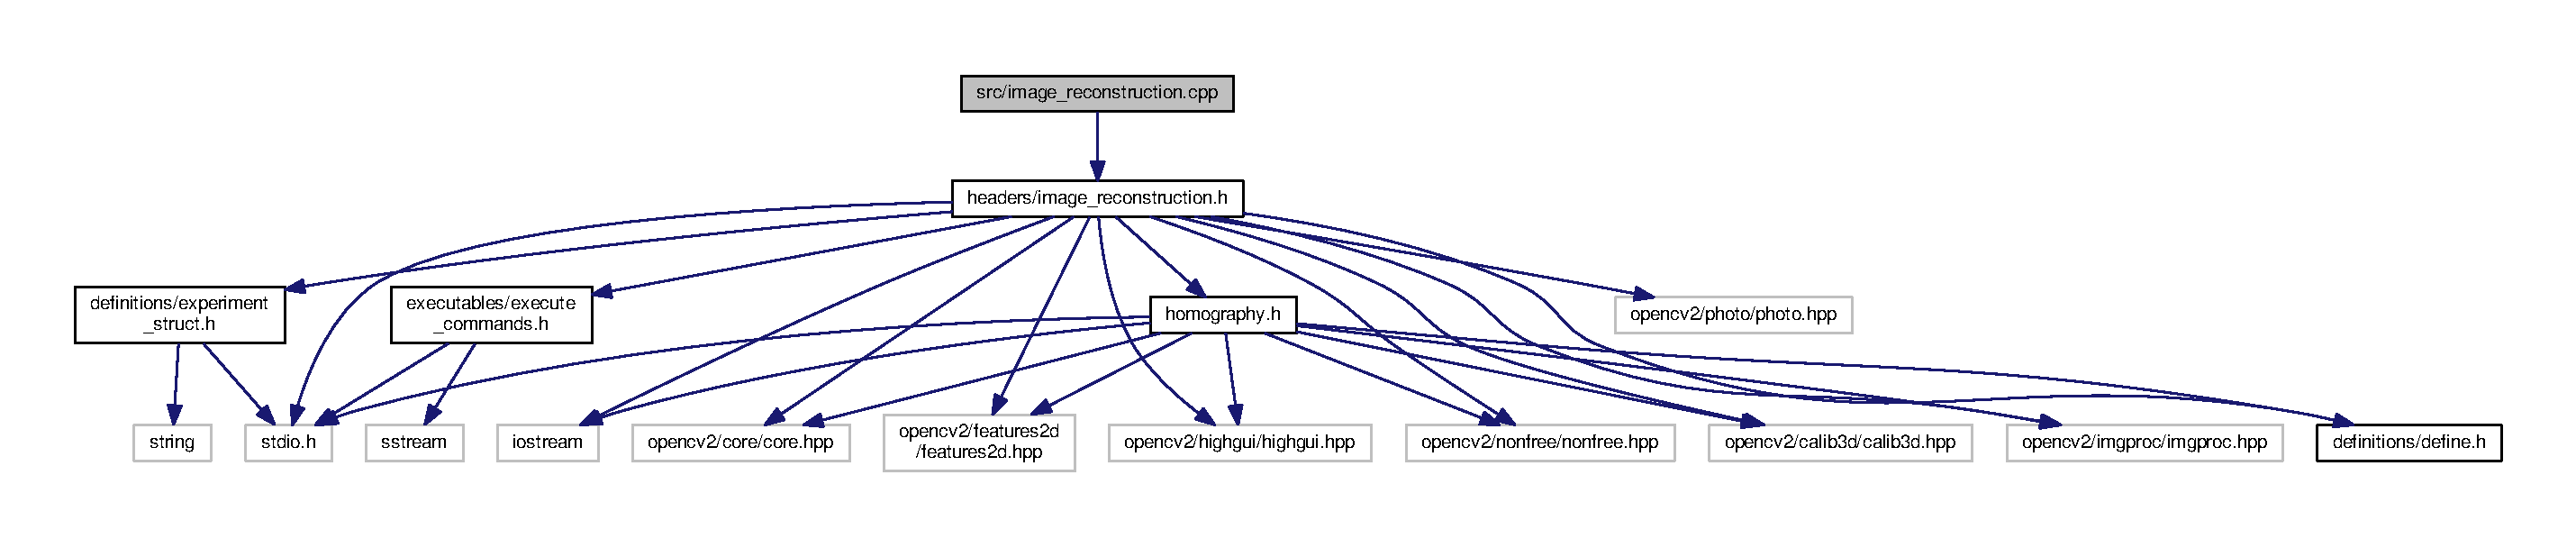
\includegraphics[width=350pt]{image__reconstruction_8cpp__incl}
\end{center}
\end{figure}
\subsection*{Functions}
\begin{DoxyCompactItemize}
\item 
bool \hyperlink{image__reconstruction_8cpp_a2fc13976a9f1af8bb9040db7de417721}{check\+Image\+Boundaries} (const cv\+::\+Mat \&image, const cv\+::\+Rect \&frame\+\_\+boundaries)
\begin{DoxyCompactList}\small\item\em Function that verify if the image fill all the frame limite given by the rect boundaries. \end{DoxyCompactList}\item 
bool \hyperlink{image__reconstruction_8cpp_a95b3fdabdd4482acec2a7f72e82eb58f}{check\+Image\+Boundaries\+Mask} (const cv\+::\+Mat \&image\+\_\+mask, const cv\+::\+Rect \&frame\+\_\+boundaries)
\begin{DoxyCompactList}\small\item\em Function that verify if the image\+\_\+mask fill all the frame limite given by the rect boundaries. \end{DoxyCompactList}\item 
bool \hyperlink{image__reconstruction_8cpp_a3808c00f0f1deb7c9669f0d30ffd63ac}{warp\+Mask\+Crop} (const cv\+::\+Mat \&image\+\_\+to\+\_\+warp, const cv\+::\+Mat \&image\+\_\+fixed, const cv\+::\+Mat \&image\+\_\+fixed\+\_\+mask, cv\+::\+Mat \&image\+\_\+result, cv\+::\+Mat \&image\+\_\+result\+\_\+mask)
\begin{DoxyCompactList}\small\item\em Function that warps the image\+\_\+to\+\_\+warp with the image image\+\_\+fixed and save the result into de image\+\_\+result and then the resut is cropped into the original image area. \end{DoxyCompactList}\item 
bool \hyperlink{image__reconstruction_8cpp_a81ebac71847f40916c2bb033ad2069be}{warp\+Mask} (const cv\+::\+Mat \&image\+\_\+to\+\_\+warp, const cv\+::\+Mat \&image\+\_\+fixed, const cv\+::\+Mat \&image\+\_\+fixed\+\_\+mask, cv\+::\+Mat \&image\+\_\+result, cv\+::\+Mat \&image\+\_\+result\+\_\+mask)
\begin{DoxyCompactList}\small\item\em Function that warps the image\+\_\+to\+\_\+warp with the image image\+\_\+fixed and save the result into de image\+\_\+result. \end{DoxyCompactList}\item 
bool \hyperlink{image__reconstruction_8cpp_a5ac0e0833abd3cb52b702e15ec99a9c2}{warp} (const cv\+::\+Mat \&image\+\_\+to\+\_\+warp, const cv\+::\+Mat \&image\+\_\+fixed, cv\+::\+Mat \&image\+\_\+result)
\begin{DoxyCompactList}\small\item\em Function that warps the image\+\_\+to\+\_\+warp with the image image\+\_\+fixed and save the result into de image\+\_\+result. \end{DoxyCompactList}\item 
bool \hyperlink{image__reconstruction_8cpp_a9e97c5996e454dcb23c2c4be119cbe31}{image\+Reconstruction} (const cv\+::\+Mat \&image, const int index, const \hyperlink{structEXPERIMENT}{E\+X\+P\+E\+R\+I\+M\+E\+NT} \&\hyperlink{main_8cpp_a9f5a81402e170475690f371d55cbe623}{experiment\+\_\+settings}, const cv\+::\+Rect \&frame\+\_\+boundaries, cv\+::\+Mat \&reconstructed\+\_\+image)
\begin{DoxyCompactList}\small\item\em Function that reconstructs an image using panorama based on homography in a image sequence. \end{DoxyCompactList}\item 
bool \hyperlink{image__reconstruction_8cpp_ad6b2680d1178aa193da11f5173c40c3c}{reconstruct\+Image} (const cv\+::\+Mat \&image, const cv\+::\+Mat \&homography\+\_\+matrix, const int index, const \hyperlink{structEXPERIMENT}{E\+X\+P\+E\+R\+I\+M\+E\+NT} \&\hyperlink{main_8cpp_a9f5a81402e170475690f371d55cbe623}{experiment\+\_\+settings}, const cv\+::\+Rect \&drop\+\_\+boundaries, const cv\+::\+Rect \&frame\+\_\+boundaries, cv\+::\+Mat \&reconstructed\+\_\+image)
\begin{DoxyCompactList}\small\item\em Function that reconstructs an image using panorama based on homography in a image sequence. \end{DoxyCompactList}\end{DoxyCompactItemize}


\subsection{Detailed Description}
Functions related with reconstruction of the image after application of the homography matrix to fill the whole frame boundaries. 

Functions to check the frame boundaries. Warp images to increase the image area. Reconstruction the image using frame from the original video. 

\subsection{Function Documentation}
\index{image\+\_\+reconstruction.\+cpp@{image\+\_\+reconstruction.\+cpp}!check\+Image\+Boundaries@{check\+Image\+Boundaries}}
\index{check\+Image\+Boundaries@{check\+Image\+Boundaries}!image\+\_\+reconstruction.\+cpp@{image\+\_\+reconstruction.\+cpp}}
\subsubsection[{\texorpdfstring{check\+Image\+Boundaries(const cv\+::\+Mat \&image, const cv\+::\+Rect \&frame\+\_\+boundaries)}{checkImageBoundaries(const cv::Mat \&image, const cv::Rect \&frame\_boundaries)}}]{\setlength{\rightskip}{0pt plus 5cm}bool check\+Image\+Boundaries (
\begin{DoxyParamCaption}
\item[{const cv\+::\+Mat \&}]{image, }
\item[{const cv\+::\+Rect \&}]{frame\+\_\+boundaries}
\end{DoxyParamCaption}
)}\hypertarget{image__reconstruction_8cpp_a2fc13976a9f1af8bb9040db7de417721}{}\label{image__reconstruction_8cpp_a2fc13976a9f1af8bb9040db7de417721}


Function that verify if the image fill all the frame limite given by the rect boundaries. 


\begin{DoxyParams}{Parameters}
{\em image} & -\/ image that will be checked. \\
\hline
{\em frame\+\_\+boundaries} & -\/ area where the image should fill.\\
\hline
\end{DoxyParams}
\begin{DoxyReturn}{Returns}
{\ttfamily bool} {\bfseries true} -\/ if the image fill all the frame limit. ~\newline
 {\ttfamily bool} {\bfseries false} -\/ if the image does not fill all the frame limit.
\end{DoxyReturn}
\begin{DoxyAuthor}{Author}
Michel Melo da Silva 
\end{DoxyAuthor}
\begin{DoxyDate}{Date}
14/04/2016 
\end{DoxyDate}
\index{image\+\_\+reconstruction.\+cpp@{image\+\_\+reconstruction.\+cpp}!check\+Image\+Boundaries\+Mask@{check\+Image\+Boundaries\+Mask}}
\index{check\+Image\+Boundaries\+Mask@{check\+Image\+Boundaries\+Mask}!image\+\_\+reconstruction.\+cpp@{image\+\_\+reconstruction.\+cpp}}
\subsubsection[{\texorpdfstring{check\+Image\+Boundaries\+Mask(const cv\+::\+Mat \&image\+\_\+mask, const cv\+::\+Rect \&frame\+\_\+boundaries)}{checkImageBoundariesMask(const cv::Mat \&image\_mask, const cv::Rect \&frame\_boundaries)}}]{\setlength{\rightskip}{0pt plus 5cm}bool check\+Image\+Boundaries\+Mask (
\begin{DoxyParamCaption}
\item[{const cv\+::\+Mat \&}]{image\+\_\+mask, }
\item[{const cv\+::\+Rect \&}]{frame\+\_\+boundaries}
\end{DoxyParamCaption}
)}\hypertarget{image__reconstruction_8cpp_a95b3fdabdd4482acec2a7f72e82eb58f}{}\label{image__reconstruction_8cpp_a95b3fdabdd4482acec2a7f72e82eb58f}


Function that verify if the image\+\_\+mask fill all the frame limite given by the rect boundaries. 


\begin{DoxyParams}{Parameters}
{\em image\+\_\+mask} & -\/ mask of the image to be checked. \\
\hline
{\em frame\+\_\+boundaries} & -\/ area where the image should fill.\\
\hline
\end{DoxyParams}
\begin{DoxyReturn}{Returns}
{\ttfamily bool} {\bfseries true} -\/ if the image fill all the frame limit. ~\newline
 {\ttfamily bool} {\bfseries false} -\/ if the image does not fill all the frame limit.
\end{DoxyReturn}
\begin{DoxyAuthor}{Author}
Michel Melo da Silva 
\end{DoxyAuthor}
\begin{DoxyDate}{Date}
03/05/2016 
\end{DoxyDate}
\index{image\+\_\+reconstruction.\+cpp@{image\+\_\+reconstruction.\+cpp}!image\+Reconstruction@{image\+Reconstruction}}
\index{image\+Reconstruction@{image\+Reconstruction}!image\+\_\+reconstruction.\+cpp@{image\+\_\+reconstruction.\+cpp}}
\subsubsection[{\texorpdfstring{image\+Reconstruction(const cv\+::\+Mat \&image, const int index, const E\+X\+P\+E\+R\+I\+M\+E\+N\+T \&experiment\+\_\+settings, const cv\+::\+Rect \&frame\+\_\+boundaries, cv\+::\+Mat \&reconstructed\+\_\+image)}{imageReconstruction(const cv::Mat \&image, const int index, const EXPERIMENT \&experiment\_settings, const cv::Rect \&frame\_boundaries, cv::Mat \&reconstructed\_image)}}]{\setlength{\rightskip}{0pt plus 5cm}bool image\+Reconstruction (
\begin{DoxyParamCaption}
\item[{const cv\+::\+Mat \&}]{image, }
\item[{const int}]{index, }
\item[{const {\bf E\+X\+P\+E\+R\+I\+M\+E\+NT} \&}]{experiment\+\_\+settings, }
\item[{const cv\+::\+Rect \&}]{frame\+\_\+boundaries, }
\item[{cv\+::\+Mat \&}]{reconstructed\+\_\+image}
\end{DoxyParamCaption}
)}\hypertarget{image__reconstruction_8cpp_a9e97c5996e454dcb23c2c4be119cbe31}{}\label{image__reconstruction_8cpp_a9e97c5996e454dcb23c2c4be119cbe31}


Function that reconstructs an image using panorama based on homography in a image sequence. 


\begin{DoxyParams}{Parameters}
{\em image} & -\/ image initial with homography transformation. \\
\hline
{\em index} & -\/ index of the initial image in the original video. \\
\hline
{\em experiment\+\_\+settings} & -\/ object with the experiment settings. \\
\hline
{\em frame\+\_\+boundaries} & -\/ limits of the frame that needs to be filled by the reconstructed image. \\
\hline
{\em reconstructed\+\_\+image} & -\/ object to save the final reconstructed image.\\
\hline
\end{DoxyParams}
\begin{DoxyReturn}{Returns}
{\ttfamily bool} {\bfseries true} -\/ if the frame was successful reconstructed filling all the frame limit. ~\newline
 {\ttfamily bool} {\bfseries false} -\/ if the frame was not successful reconstructed filling all the frame limit.
\end{DoxyReturn}
\begin{DoxyAuthor}{Author}
Michel Melo da Silva 
\end{DoxyAuthor}
\begin{DoxyDate}{Date}
14/04/2016 
\end{DoxyDate}
\index{image\+\_\+reconstruction.\+cpp@{image\+\_\+reconstruction.\+cpp}!reconstruct\+Image@{reconstruct\+Image}}
\index{reconstruct\+Image@{reconstruct\+Image}!image\+\_\+reconstruction.\+cpp@{image\+\_\+reconstruction.\+cpp}}
\subsubsection[{\texorpdfstring{reconstruct\+Image(const cv\+::\+Mat \&image, const cv\+::\+Mat \&homography\+\_\+matrix, const int index, const E\+X\+P\+E\+R\+I\+M\+E\+N\+T \&experiment\+\_\+settings, const cv\+::\+Rect \&drop\+\_\+boundaries, const cv\+::\+Rect \&frame\+\_\+boundaries, cv\+::\+Mat \&reconstructed\+\_\+image)}{reconstructImage(const cv::Mat \&image, const cv::Mat \&homography\_matrix, const int index, const EXPERIMENT \&experiment\_settings, const cv::Rect \&drop\_boundaries, const cv::Rect \&frame\_boundaries, cv::Mat \&reconstructed\_image)}}]{\setlength{\rightskip}{0pt plus 5cm}bool reconstruct\+Image (
\begin{DoxyParamCaption}
\item[{const cv\+::\+Mat \&}]{image, }
\item[{const cv\+::\+Mat \&}]{homography\+\_\+matrix, }
\item[{const int}]{index, }
\item[{const {\bf E\+X\+P\+E\+R\+I\+M\+E\+NT} \&}]{experiment\+\_\+settings, }
\item[{const cv\+::\+Rect \&}]{drop\+\_\+boundaries, }
\item[{const cv\+::\+Rect \&}]{frame\+\_\+boundaries, }
\item[{cv\+::\+Mat \&}]{reconstructed\+\_\+image}
\end{DoxyParamCaption}
)}\hypertarget{image__reconstruction_8cpp_ad6b2680d1178aa193da11f5173c40c3c}{}\label{image__reconstruction_8cpp_ad6b2680d1178aa193da11f5173c40c3c}


Function that reconstructs an image using panorama based on homography in a image sequence. 


\begin{DoxyParams}{Parameters}
{\em image} & -\/ image initial without homography transformation. \\
\hline
{\em homography\+\_\+matrix} & -\/ homography matrix that will be applied to the original image where the reconstruct will start. \\
\hline
{\em index} & -\/ index of the initial image in the original video. \\
\hline
{\em experiment\+\_\+settings} & -\/ object with the experiment settings. \\
\hline
{\em frame\+\_\+boundaries} & -\/ limits of the frame that needs to be filled by the reconstructed image. \\
\hline
{\em reconstructed\+\_\+image} & -\/ object to save the final reconstructed image.\\
\hline
\end{DoxyParams}
\begin{DoxyReturn}{Returns}
{\ttfamily bool} {\bfseries true} -\/ if the frame was successful reconstructed filling all the frame limit. ~\newline
 {\ttfamily bool} {\bfseries false} -\/ if the frame was not successful reconstructed filling all the frame limit.
\end{DoxyReturn}
\begin{DoxyAuthor}{Author}
Michel Melo da Silva 
\end{DoxyAuthor}
\begin{DoxyDate}{Date}
14/04/2016 
\end{DoxyDate}
\index{image\+\_\+reconstruction.\+cpp@{image\+\_\+reconstruction.\+cpp}!warp@{warp}}
\index{warp@{warp}!image\+\_\+reconstruction.\+cpp@{image\+\_\+reconstruction.\+cpp}}
\subsubsection[{\texorpdfstring{warp(const cv\+::\+Mat \&image\+\_\+to\+\_\+warp, const cv\+::\+Mat \&image\+\_\+fixed, cv\+::\+Mat \&image\+\_\+result)}{warp(const cv::Mat \&image\_to\_warp, const cv::Mat \&image\_fixed, cv::Mat \&image\_result)}}]{\setlength{\rightskip}{0pt plus 5cm}bool warp (
\begin{DoxyParamCaption}
\item[{const cv\+::\+Mat \&}]{image\+\_\+to\+\_\+warp, }
\item[{const cv\+::\+Mat \&}]{image\+\_\+fixed, }
\item[{cv\+::\+Mat \&}]{image\+\_\+result}
\end{DoxyParamCaption}
)}\hypertarget{image__reconstruction_8cpp_a5ac0e0833abd3cb52b702e15ec99a9c2}{}\label{image__reconstruction_8cpp_a5ac0e0833abd3cb52b702e15ec99a9c2}


Function that warps the image\+\_\+to\+\_\+warp with the image image\+\_\+fixed and save the result into de image\+\_\+result. 


\begin{DoxyParams}{Parameters}
{\em image\+\_\+to\+\_\+warp} & -\/ image to warp. \\
\hline
{\em image\+\_\+fixed} & -\/ image fixed that will be in the first plane. \\
\hline
{\em image\+\_\+result} & -\/ object to save the result image.\\
\hline
\end{DoxyParams}
\begin{DoxyReturn}{Returns}
{\ttfamily bool} {\bfseries true} -\/ if the corner consistency is maintained after application of the homography matrix found to warp the image. It also returns false if is not found a homography matrix between the images. ~\newline
 {\ttfamily bool} {\bfseries false} -\/ if the consistency is not maintained after application of the homography matrix found to warp the image. In this case the image\+Result is a simple copy of the image\+Fixed.
\end{DoxyReturn}
\begin{DoxyAuthor}{Author}
Michel Melo da Silva 
\end{DoxyAuthor}
\begin{DoxyDate}{Date}
14/11/2015 
\end{DoxyDate}
\index{image\+\_\+reconstruction.\+cpp@{image\+\_\+reconstruction.\+cpp}!warp\+Mask@{warp\+Mask}}
\index{warp\+Mask@{warp\+Mask}!image\+\_\+reconstruction.\+cpp@{image\+\_\+reconstruction.\+cpp}}
\subsubsection[{\texorpdfstring{warp\+Mask(const cv\+::\+Mat \&image\+\_\+to\+\_\+warp, const cv\+::\+Mat \&image\+\_\+fixed, const cv\+::\+Mat \&image\+\_\+fixed\+\_\+mask, cv\+::\+Mat \&image\+\_\+result, cv\+::\+Mat \&image\+\_\+result\+\_\+mask)}{warpMask(const cv::Mat \&image\_to\_warp, const cv::Mat \&image\_fixed, const cv::Mat \&image\_fixed\_mask, cv::Mat \&image\_result, cv::Mat \&image\_result\_mask)}}]{\setlength{\rightskip}{0pt plus 5cm}bool warp\+Mask (
\begin{DoxyParamCaption}
\item[{const cv\+::\+Mat \&}]{image\+\_\+to\+\_\+warp, }
\item[{const cv\+::\+Mat \&}]{image\+\_\+fixed, }
\item[{const cv\+::\+Mat \&}]{image\+\_\+fixed\+\_\+mask, }
\item[{cv\+::\+Mat \&}]{image\+\_\+result, }
\item[{cv\+::\+Mat \&}]{image\+\_\+result\+\_\+mask}
\end{DoxyParamCaption}
)}\hypertarget{image__reconstruction_8cpp_a81ebac71847f40916c2bb033ad2069be}{}\label{image__reconstruction_8cpp_a81ebac71847f40916c2bb033ad2069be}


Function that warps the image\+\_\+to\+\_\+warp with the image image\+\_\+fixed and save the result into de image\+\_\+result. 


\begin{DoxyParams}{Parameters}
{\em image\+\_\+to\+\_\+warp} & -\/ image to warp. \\
\hline
{\em image\+\_\+fixed} & -\/ image fixed that will be in the first plane. \\
\hline
{\em image\+\_\+fixed\+\_\+mask} & -\/ mask of the fixed mask. \\
\hline
{\em image\+\_\+result} & -\/ object to save the result image. \\
\hline
{\em image\+\_\+result\+\_\+mask} & -\/ objecto to save the mask of the result image.\\
\hline
\end{DoxyParams}
\begin{DoxyReturn}{Returns}
{\ttfamily bool} {\bfseries true} -\/ if the corner consistency is maintained after application of the homography matrix found to warp the image. It also returns false if is not found a homography matrix between the images. ~\newline
 {\ttfamily bool} {\bfseries false} -\/ if the consistency is not maintained after application of the homography matrix found to warp the image. In this case the image\+Result is a simple copy of the image\+Fixed. 
\end{DoxyReturn}
\begin{DoxyAuthor}{Author}
Michel Melo da Silva 
\end{DoxyAuthor}
\begin{DoxyDate}{Date}
20/04/2016 
\end{DoxyDate}
\index{image\+\_\+reconstruction.\+cpp@{image\+\_\+reconstruction.\+cpp}!warp\+Mask\+Crop@{warp\+Mask\+Crop}}
\index{warp\+Mask\+Crop@{warp\+Mask\+Crop}!image\+\_\+reconstruction.\+cpp@{image\+\_\+reconstruction.\+cpp}}
\subsubsection[{\texorpdfstring{warp\+Mask\+Crop(const cv\+::\+Mat \&image\+\_\+to\+\_\+warp, const cv\+::\+Mat \&image\+\_\+fixed, const cv\+::\+Mat \&image\+\_\+fixed\+\_\+mask, cv\+::\+Mat \&image\+\_\+result, cv\+::\+Mat \&image\+\_\+result\+\_\+mask)}{warpMaskCrop(const cv::Mat \&image\_to\_warp, const cv::Mat \&image\_fixed, const cv::Mat \&image\_fixed\_mask, cv::Mat \&image\_result, cv::Mat \&image\_result\_mask)}}]{\setlength{\rightskip}{0pt plus 5cm}bool warp\+Mask\+Crop (
\begin{DoxyParamCaption}
\item[{const cv\+::\+Mat \&}]{image\+\_\+to\+\_\+warp, }
\item[{const cv\+::\+Mat \&}]{image\+\_\+fixed, }
\item[{const cv\+::\+Mat \&}]{image\+\_\+fixed\+\_\+mask, }
\item[{cv\+::\+Mat \&}]{image\+\_\+result, }
\item[{cv\+::\+Mat \&}]{image\+\_\+result\+\_\+mask}
\end{DoxyParamCaption}
)}\hypertarget{image__reconstruction_8cpp_a3808c00f0f1deb7c9669f0d30ffd63ac}{}\label{image__reconstruction_8cpp_a3808c00f0f1deb7c9669f0d30ffd63ac}


Function that warps the image\+\_\+to\+\_\+warp with the image image\+\_\+fixed and save the result into de image\+\_\+result and then the resut is cropped into the original image area. 


\begin{DoxyParams}{Parameters}
{\em image\+\_\+to\+\_\+warp} & -\/ image to warp. \\
\hline
{\em image\+\_\+fixed} & -\/ image fixed that will be in the first plane. \\
\hline
{\em image\+\_\+fixed\+\_\+mask} & -\/ mask of the fixed mask. \\
\hline
{\em image\+\_\+result} & -\/ object to save the result image. \\
\hline
{\em image\+\_\+result\+\_\+mask} & -\/ objecto to save the mask of the result image.\\
\hline
\end{DoxyParams}
\begin{DoxyReturn}{Returns}
{\ttfamily bool} {\bfseries true} -\/ if the corner consistency is maintained after application of the homography matrix found to warp the image. It also returns false if is not found a homography matrix between the images. ~\newline
 {\ttfamily bool} {\bfseries false} -\/ if the consistency is not maintained after application of the homography matrix found to warp the image. In this case the image\+Result is a simple copy of the image\+Fixed.
\end{DoxyReturn}
\begin{DoxyAuthor}{Author}
Michel Melo da Silva 
\end{DoxyAuthor}
\begin{DoxyDate}{Date}
03/05/2016 
\end{DoxyDate}

\hypertarget{line__and__point__operations_8cpp}{}\section{src/line\+\_\+and\+\_\+point\+\_\+operations.cpp File Reference}
\label{line__and__point__operations_8cpp}\index{src/line\+\_\+and\+\_\+point\+\_\+operations.\+cpp@{src/line\+\_\+and\+\_\+point\+\_\+operations.\+cpp}}


Functions to handle line and point functions.  


{\ttfamily \#include \char`\"{}headers/line\+\_\+and\+\_\+point\+\_\+operations.\+h\char`\"{}}\\*
Include dependency graph for line\+\_\+and\+\_\+point\+\_\+operations.\+cpp\+:\nopagebreak
\begin{figure}[H]
\begin{center}
\leavevmode
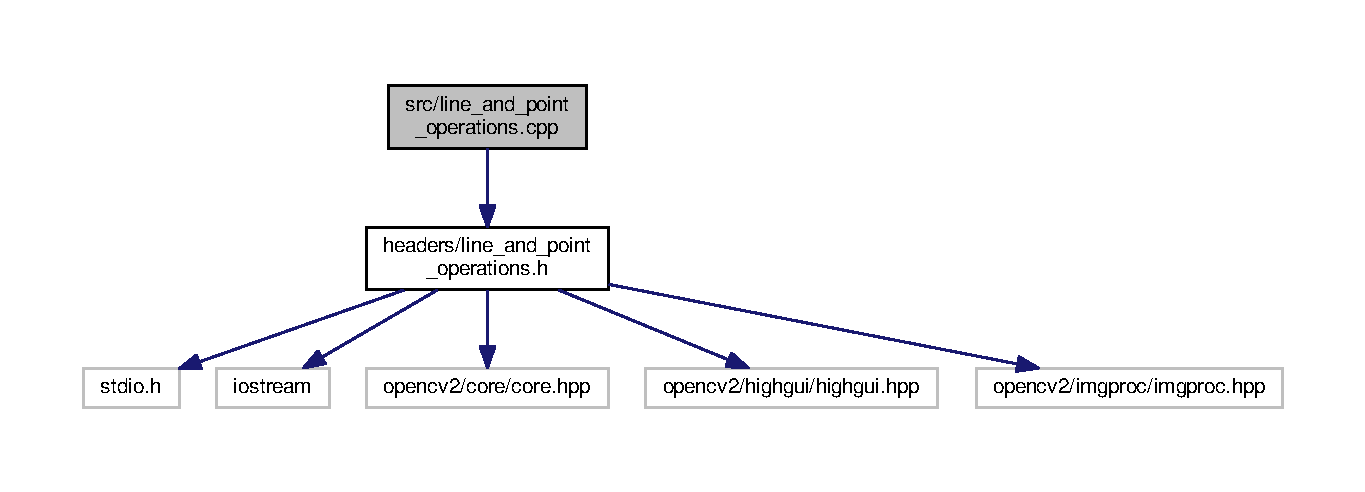
\includegraphics[width=350pt]{line__and__point__operations_8cpp__incl}
\end{center}
\end{figure}
\subsection*{Functions}
\begin{DoxyCompactItemize}
\item 
bool \hyperlink{line__and__point__operations_8cpp_a6263aa9bb1b8d1a66ab24e33b3649668}{line\+Segment\+Intersection} (const cv\+::\+Point2f \&a1, const cv\+::\+Point2f \&b1, const cv\+::\+Point2f \&a2, const cv\+::\+Point2f \&b2)
\begin{DoxyCompactList}\small\item\em Function that verify if two line segments have intersection point. \end{DoxyCompactList}\item 
bool \hyperlink{line__and__point__operations_8cpp_aa6722cd85e8b9ffbbeb447c179fd0bae}{line\+Segment\+Intersection} (const cv\+::\+Point2f \&a1, const cv\+::\+Point2f \&b1, const cv\+::\+Point2f \&a2, const cv\+::\+Point2f \&b2, cv\+::\+Point2f \&intersection)
\begin{DoxyCompactList}\small\item\em Function that calculate the homography matrix that leave the frame\+\_\+i to the intermediate plan between the plans of frame\+\_\+master\+\_\+pre and frame\+\_\+master\+\_\+pre with relation of the distance between them. \end{DoxyCompactList}\item 
void \hyperlink{line__and__point__operations_8cpp_ae4a4317f4956ee9fa08d3e6445917f4f}{compute\+Angles\+And\+Mags} (const std\+::vector$<$ cv\+::\+Point2f $>$ \&points\+\_\+src, const std\+::vector$<$ cv\+::\+Point2f $>$ \&points\+\_\+dst, std\+::vector$<$ float $>$ \&angles, std\+::vector$<$ float $>$ \&mags)
\begin{DoxyCompactList}\small\item\em Function that compute the angle and magnitude of the optical flow from the points\+\_\+src to points\+\_\+dst. \end{DoxyCompactList}\end{DoxyCompactItemize}


\subsection{Detailed Description}
Functions to handle line and point functions. 

Functions to find lines and segment line intersection. Compute angle and magnitude of vectors. 

\subsection{Function Documentation}
\index{line\+\_\+and\+\_\+point\+\_\+operations.\+cpp@{line\+\_\+and\+\_\+point\+\_\+operations.\+cpp}!compute\+Angles\+And\+Mags@{compute\+Angles\+And\+Mags}}
\index{compute\+Angles\+And\+Mags@{compute\+Angles\+And\+Mags}!line\+\_\+and\+\_\+point\+\_\+operations.\+cpp@{line\+\_\+and\+\_\+point\+\_\+operations.\+cpp}}
\subsubsection[{\texorpdfstring{compute\+Angles\+And\+Mags(const std\+::vector$<$ cv\+::\+Point2f $>$ \&points\+\_\+src, const std\+::vector$<$ cv\+::\+Point2f $>$ \&points\+\_\+dst, std\+::vector$<$ float $>$ \&angles, std\+::vector$<$ float $>$ \&mags)}{computeAnglesAndMags(const std::vector< cv::Point2f > \&points\_src, const std::vector< cv::Point2f > \&points\_dst, std::vector< float > \&angles, std::vector< float > \&mags)}}]{\setlength{\rightskip}{0pt plus 5cm}void compute\+Angles\+And\+Mags (
\begin{DoxyParamCaption}
\item[{const std\+::vector$<$ cv\+::\+Point2f $>$ \&}]{points\+\_\+src, }
\item[{const std\+::vector$<$ cv\+::\+Point2f $>$ \&}]{points\+\_\+dst, }
\item[{std\+::vector$<$ float $>$ \&}]{angles, }
\item[{std\+::vector$<$ float $>$ \&}]{mags}
\end{DoxyParamCaption}
)}\hypertarget{line__and__point__operations_8cpp_ae4a4317f4956ee9fa08d3e6445917f4f}{}\label{line__and__point__operations_8cpp_ae4a4317f4956ee9fa08d3e6445917f4f}


Function that compute the angle and magnitude of the optical flow from the points\+\_\+src to points\+\_\+dst. 


\begin{DoxyParams}{Parameters}
{\em points\+\_\+src} & -\/ vector of source points. \\
\hline
{\em points\+\_\+dst} & -\/ vector of destination points. \\
\hline
{\em angles} & -\/ object to save the angle of the vectors. \\
\hline
{\em mags} & -\/ object to save the magnitude of the vectors.\\
\hline
\end{DoxyParams}
\begin{DoxyReturn}{Returns}
{\ttfamily void} 
\end{DoxyReturn}
\begin{DoxyAuthor}{Author}
Washington Luis de Souza Ramos 
\end{DoxyAuthor}
\begin{DoxyDate}{Date}
10/04/2016 
\end{DoxyDate}
\index{line\+\_\+and\+\_\+point\+\_\+operations.\+cpp@{line\+\_\+and\+\_\+point\+\_\+operations.\+cpp}!line\+Segment\+Intersection@{line\+Segment\+Intersection}}
\index{line\+Segment\+Intersection@{line\+Segment\+Intersection}!line\+\_\+and\+\_\+point\+\_\+operations.\+cpp@{line\+\_\+and\+\_\+point\+\_\+operations.\+cpp}}
\subsubsection[{\texorpdfstring{line\+Segment\+Intersection(const cv\+::\+Point2f \&a1, const cv\+::\+Point2f \&b1, const cv\+::\+Point2f \&a2, const cv\+::\+Point2f \&b2)}{lineSegmentIntersection(const cv::Point2f \&a1, const cv::Point2f \&b1, const cv::Point2f \&a2, const cv::Point2f \&b2)}}]{\setlength{\rightskip}{0pt plus 5cm}bool line\+Segment\+Intersection (
\begin{DoxyParamCaption}
\item[{const cv\+::\+Point2f \&}]{a1, }
\item[{const cv\+::\+Point2f \&}]{b1, }
\item[{const cv\+::\+Point2f \&}]{a2, }
\item[{const cv\+::\+Point2f \&}]{b2}
\end{DoxyParamCaption}
)}\hypertarget{line__and__point__operations_8cpp_a6263aa9bb1b8d1a66ab24e33b3649668}{}\label{line__and__point__operations_8cpp_a6263aa9bb1b8d1a66ab24e33b3649668}


Function that verify if two line segments have intersection point. 

\begin{DoxySeeAlso}{See also}
\href{https://github.com/Itseez/opencv/blob/master/modules/imgproc/src/min_enclosing_triangle.cpp}{\tt https\+://github.\+com/\+Itseez/opencv/blob/master/modules/imgproc/src/min\+\_\+enclosing\+\_\+triangle.\+cpp}
\end{DoxySeeAlso}

\begin{DoxyParams}{Parameters}
{\em a1} & -\/ first point of the first line segment. \\
\hline
{\em b1} & -\/ second point of the first line segment. \\
\hline
{\em a2} & -\/ first point of the second line segment. \\
\hline
{\em b2} & -\/ second point of the second line segment.\\
\hline
\end{DoxyParams}
\begin{DoxyReturn}{Returns}
{\ttfamily bool} {\bfseries true} -\/ if there is a intersection point. ~\newline
 {\ttfamily bool} {\bfseries false} -\/ if there is not a intersection point.
\end{DoxyReturn}
\begin{DoxyAuthor}{Author}
Michel Melo da Silva 
\end{DoxyAuthor}
\begin{DoxyDate}{Date}
04/04/2016 
\end{DoxyDate}
\index{line\+\_\+and\+\_\+point\+\_\+operations.\+cpp@{line\+\_\+and\+\_\+point\+\_\+operations.\+cpp}!line\+Segment\+Intersection@{line\+Segment\+Intersection}}
\index{line\+Segment\+Intersection@{line\+Segment\+Intersection}!line\+\_\+and\+\_\+point\+\_\+operations.\+cpp@{line\+\_\+and\+\_\+point\+\_\+operations.\+cpp}}
\subsubsection[{\texorpdfstring{line\+Segment\+Intersection(const cv\+::\+Point2f \&a1, const cv\+::\+Point2f \&b1, const cv\+::\+Point2f \&a2, const cv\+::\+Point2f \&b2, cv\+::\+Point2f \&intersection)}{lineSegmentIntersection(const cv::Point2f \&a1, const cv::Point2f \&b1, const cv::Point2f \&a2, const cv::Point2f \&b2, cv::Point2f \&intersection)}}]{\setlength{\rightskip}{0pt plus 5cm}bool line\+Segment\+Intersection (
\begin{DoxyParamCaption}
\item[{const cv\+::\+Point2f \&}]{a1, }
\item[{const cv\+::\+Point2f \&}]{b1, }
\item[{const cv\+::\+Point2f \&}]{a2, }
\item[{const cv\+::\+Point2f \&}]{b2, }
\item[{cv\+::\+Point2f \&}]{intersection}
\end{DoxyParamCaption}
)}\hypertarget{line__and__point__operations_8cpp_aa6722cd85e8b9ffbbeb447c179fd0bae}{}\label{line__and__point__operations_8cpp_aa6722cd85e8b9ffbbeb447c179fd0bae}


Function that calculate the homography matrix that leave the frame\+\_\+i to the intermediate plan between the plans of frame\+\_\+master\+\_\+pre and frame\+\_\+master\+\_\+pre with relation of the distance between them. 

\begin{DoxySeeAlso}{See also}
\href{https://github.com/Itseez/opencv/blob/master/modules/imgproc/src/min_enclosing_triangle.cpp}{\tt https\+://github.\+com/\+Itseez/opencv/blob/master/modules/imgproc/src/min\+\_\+enclosing\+\_\+triangle.\+cpp}
\end{DoxySeeAlso}

\begin{DoxyParams}{Parameters}
{\em a1} & -\/ first point of the first line segment. \\
\hline
{\em b1} & -\/ second point of the first line segment. \\
\hline
{\em a2} & -\/ first point of the second line segment. \\
\hline
{\em b2} & -\/ second point of the second line segment. \\
\hline
{\em intersection} & -\/ intersection point between the line segments.\\
\hline
\end{DoxyParams}
\begin{DoxyReturn}{Returns}
{\ttfamily bool} {\bfseries true} -\/ if there is a intersection point. ~\newline
 {\ttfamily bool} {\bfseries false} -\/ if there is not a intersection point.
\end{DoxyReturn}
\begin{DoxyAuthor}{Author}
Michel Melo da Silva 
\end{DoxyAuthor}
\begin{DoxyDate}{Date}
04/04/2016 
\end{DoxyDate}

\hypertarget{line__and__points__operations_8cpp}{}\section{src/line\+\_\+and\+\_\+points\+\_\+operations.cpp File Reference}
\label{line__and__points__operations_8cpp}\index{src/line\+\_\+and\+\_\+points\+\_\+operations.\+cpp@{src/line\+\_\+and\+\_\+points\+\_\+operations.\+cpp}}
{\ttfamily \#include \char`\"{}headers/line\+\_\+and\+\_\+points\+\_\+operations.\+h\char`\"{}}\\*
Include dependency graph for line\+\_\+and\+\_\+points\+\_\+operations.\+cpp\+:\nopagebreak
\begin{figure}[H]
\begin{center}
\leavevmode
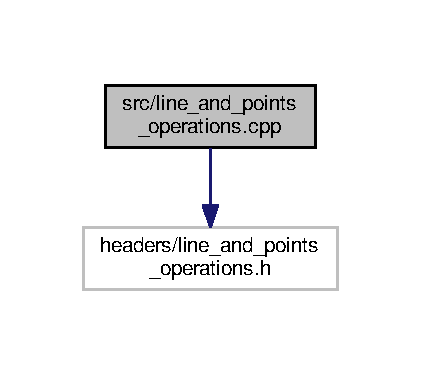
\includegraphics[width=202pt]{line__and__points__operations_8cpp__incl}
\end{center}
\end{figure}
\subsection*{Functions}
\begin{Indent}{\bf find\+Intermediate\+Homography\+Matrix}\par
{\em Function that returns the maximum of the three provided numbers.

https\+://github.com/\+Itseez/opencv/blob/master/modules/imgproc/src/min\+\_\+enclosing\+\_\+triangle.\+cpp


\begin{DoxyParams}{Parameters}
{\em double} & number1 \\
\hline
{\em double} & number2 \\
\hline
{\em double} & number3\\
\hline
\end{DoxyParams}
\begin{DoxyReturn}{Returns}
double maximum
\end{DoxyReturn}
\begin{DoxyAuthor}{Author}
Itseez 
\end{DoxyAuthor}
\begin{DoxyDate}{Date}
08/04/2016 
\end{DoxyDate}
}\end{Indent}
\begin{Indent}{\bf line\+Segment\+Intersection}\par
{\em Function that calculate the homography matrix that leave the frame\+\_\+i to the intermediate plan between the plans of frame\+\_\+master\+\_\+pre and frame\+\_\+master\+\_\+pre with relation of the distance between them.

https\+://github.com/\+Itseez/opencv/blob/master/modules/imgproc/src/min\+\_\+enclosing\+\_\+triangle.\+cpp


\begin{DoxyParams}{Parameters}
{\em const} & cv\+::\+Point2f a1 -\/ first point of the first line segment \\
\hline
{\em const} & cv\+::\+Point2f b1 -\/ second point of the first line segment \\
\hline
{\em const} & cv\+::\+Point2f a2 -\/ first point of the second line segment \\
\hline
{\em const} & cv\+::\+Point2f b2 -\/ second point of the second line segment \\
\hline
{\em const} & cv\+::\+Point2f intersection -\/ intersection point between the line segments\\
\hline
\end{DoxyParams}
\begin{DoxyReturn}{Returns}
bool true -\/ if there is a intersection point. false -\/ if there is not a intersection point.
\end{DoxyReturn}
\begin{DoxyAuthor}{Author}
Michel Melo da Silva 
\end{DoxyAuthor}
\begin{DoxyDate}{Date}
04/04/2016 
\end{DoxyDate}
}\begin{DoxyCompactItemize}
\item 
bool \hyperlink{line__and__points__operations_8cpp_a6263aa9bb1b8d1a66ab24e33b3649668}{line\+Segment\+Intersection} (const cv\+::\+Point2f \&a1, const cv\+::\+Point2f \&b1, const cv\+::\+Point2f \&a2, const cv\+::\+Point2f \&b2)
\begin{DoxyCompactList}\small\item\em Function that verify if two line segments have intersection point. \end{DoxyCompactList}\item 
bool \hyperlink{line__and__points__operations_8cpp_aa6722cd85e8b9ffbbeb447c179fd0bae}{line\+Segment\+Intersection} (const cv\+::\+Point2f \&a1, const cv\+::\+Point2f \&b1, const cv\+::\+Point2f \&a2, const cv\+::\+Point2f \&b2, cv\+::\+Point2f \&intersection)
\begin{DoxyCompactList}\small\item\em Function that calculate the homography matrix that leave the frame\+\_\+i to the intermediate plan between the plans of frame\+\_\+master\+\_\+pre and frame\+\_\+master\+\_\+pre with relation of the distance between them. \end{DoxyCompactList}\end{DoxyCompactItemize}
\end{Indent}
\begin{Indent}{\bf compute\+Angles\+And\+Mags}\par
{\em Function that compute the angle and magnitude of the optical flow from the points\+\_\+src to points\+\_\+dst.


\begin{DoxyParams}{Parameters}
{\em std\+::vector$<$cv\+::\+Point2f$>$\&} & points\+\_\+src \\
\hline
{\em std\+::vector$<$cv\+::\+Point2f$>$\&} & points\+\_\+dst \\
\hline
{\em std\+::vector$<$float$>$\&} & angles \\
\hline
{\em std\+::vector$<$float$>$\&} & mags\\
\hline
\end{DoxyParams}
\begin{DoxyReturn}{Returns}
void
\end{DoxyReturn}
\begin{DoxyAuthor}{Author}
Washington Luis de Souza Ramos 
\end{DoxyAuthor}
\begin{DoxyDate}{Date}
10/04/2016 
\end{DoxyDate}
}\begin{DoxyCompactItemize}
\item 
void \hyperlink{line__and__points__operations_8cpp_ae4a4317f4956ee9fa08d3e6445917f4f}{compute\+Angles\+And\+Mags} (const std\+::vector$<$ cv\+::\+Point2f $>$ \&points\+\_\+src, const std\+::vector$<$ cv\+::\+Point2f $>$ \&points\+\_\+dst, std\+::vector$<$ float $>$ \&angles, std\+::vector$<$ float $>$ \&mags)
\begin{DoxyCompactList}\small\item\em Function that compute the angle and magnitude of the optical flow from the points\+\_\+src to points\+\_\+dst. \end{DoxyCompactList}\end{DoxyCompactItemize}
\end{Indent}


\subsection{Function Documentation}
\index{line\+\_\+and\+\_\+points\+\_\+operations.\+cpp@{line\+\_\+and\+\_\+points\+\_\+operations.\+cpp}!compute\+Angles\+And\+Mags@{compute\+Angles\+And\+Mags}}
\index{compute\+Angles\+And\+Mags@{compute\+Angles\+And\+Mags}!line\+\_\+and\+\_\+points\+\_\+operations.\+cpp@{line\+\_\+and\+\_\+points\+\_\+operations.\+cpp}}
\subsubsection[{\texorpdfstring{compute\+Angles\+And\+Mags(const std\+::vector$<$ cv\+::\+Point2f $>$ \&points\+\_\+src, const std\+::vector$<$ cv\+::\+Point2f $>$ \&points\+\_\+dst, std\+::vector$<$ float $>$ \&angles, std\+::vector$<$ float $>$ \&mags)}{computeAnglesAndMags(const std::vector< cv::Point2f > \&points\_src, const std::vector< cv::Point2f > \&points\_dst, std::vector< float > \&angles, std::vector< float > \&mags)}}]{\setlength{\rightskip}{0pt plus 5cm}void compute\+Angles\+And\+Mags (
\begin{DoxyParamCaption}
\item[{const std\+::vector$<$ cv\+::\+Point2f $>$ \&}]{points\+\_\+src, }
\item[{const std\+::vector$<$ cv\+::\+Point2f $>$ \&}]{points\+\_\+dst, }
\item[{std\+::vector$<$ float $>$ \&}]{angles, }
\item[{std\+::vector$<$ float $>$ \&}]{mags}
\end{DoxyParamCaption}
)}\hypertarget{line__and__points__operations_8cpp_ae4a4317f4956ee9fa08d3e6445917f4f}{}\label{line__and__points__operations_8cpp_ae4a4317f4956ee9fa08d3e6445917f4f}


Function that compute the angle and magnitude of the optical flow from the points\+\_\+src to points\+\_\+dst. 


\begin{DoxyParams}{Parameters}
{\em points\+\_\+src} & -\/ vector of source points. \\
\hline
{\em points\+\_\+dst} & -\/ vector of destination points. \\
\hline
{\em angles} & -\/ object to save the angle of the vectors. \\
\hline
{\em mags} & -\/ object to save the magnitude of the vectors.\\
\hline
\end{DoxyParams}
\begin{DoxyReturn}{Returns}
{\ttfamily void} 
\end{DoxyReturn}
\begin{DoxyAuthor}{Author}
Washington Luis de Souza Ramos 
\end{DoxyAuthor}
\begin{DoxyDate}{Date}
10/04/2016 
\end{DoxyDate}
\index{line\+\_\+and\+\_\+points\+\_\+operations.\+cpp@{line\+\_\+and\+\_\+points\+\_\+operations.\+cpp}!line\+Segment\+Intersection@{line\+Segment\+Intersection}}
\index{line\+Segment\+Intersection@{line\+Segment\+Intersection}!line\+\_\+and\+\_\+points\+\_\+operations.\+cpp@{line\+\_\+and\+\_\+points\+\_\+operations.\+cpp}}
\subsubsection[{\texorpdfstring{line\+Segment\+Intersection(const cv\+::\+Point2f \&a1, const cv\+::\+Point2f \&b1, const cv\+::\+Point2f \&a2, const cv\+::\+Point2f \&b2)}{lineSegmentIntersection(const cv::Point2f \&a1, const cv::Point2f \&b1, const cv::Point2f \&a2, const cv::Point2f \&b2)}}]{\setlength{\rightskip}{0pt plus 5cm}bool line\+Segment\+Intersection (
\begin{DoxyParamCaption}
\item[{const cv\+::\+Point2f \&}]{a1, }
\item[{const cv\+::\+Point2f \&}]{b1, }
\item[{const cv\+::\+Point2f \&}]{a2, }
\item[{const cv\+::\+Point2f \&}]{b2}
\end{DoxyParamCaption}
)}\hypertarget{line__and__points__operations_8cpp_a6263aa9bb1b8d1a66ab24e33b3649668}{}\label{line__and__points__operations_8cpp_a6263aa9bb1b8d1a66ab24e33b3649668}


Function that verify if two line segments have intersection point. 

\begin{DoxySeeAlso}{See also}
\href{https://github.com/Itseez/opencv/blob/master/modules/imgproc/src/min_enclosing_triangle.cpp}{\tt https\+://github.\+com/\+Itseez/opencv/blob/master/modules/imgproc/src/min\+\_\+enclosing\+\_\+triangle.\+cpp}
\end{DoxySeeAlso}

\begin{DoxyParams}{Parameters}
{\em a1} & -\/ first point of the first line segment. \\
\hline
{\em b1} & -\/ second point of the first line segment. \\
\hline
{\em a2} & -\/ first point of the second line segment. \\
\hline
{\em b2} & -\/ second point of the second line segment.\\
\hline
\end{DoxyParams}
\begin{DoxyReturn}{Returns}
{\ttfamily bool} {\bfseries true} -\/ if there is a intersection point. ~\newline
 {\ttfamily bool} {\bfseries false} -\/ if there is not a intersection point.
\end{DoxyReturn}
\begin{DoxyAuthor}{Author}
Michel Melo da Silva 
\end{DoxyAuthor}
\begin{DoxyDate}{Date}
04/04/2016 
\end{DoxyDate}
\index{line\+\_\+and\+\_\+points\+\_\+operations.\+cpp@{line\+\_\+and\+\_\+points\+\_\+operations.\+cpp}!line\+Segment\+Intersection@{line\+Segment\+Intersection}}
\index{line\+Segment\+Intersection@{line\+Segment\+Intersection}!line\+\_\+and\+\_\+points\+\_\+operations.\+cpp@{line\+\_\+and\+\_\+points\+\_\+operations.\+cpp}}
\subsubsection[{\texorpdfstring{line\+Segment\+Intersection(const cv\+::\+Point2f \&a1, const cv\+::\+Point2f \&b1, const cv\+::\+Point2f \&a2, const cv\+::\+Point2f \&b2, cv\+::\+Point2f \&intersection)}{lineSegmentIntersection(const cv::Point2f \&a1, const cv::Point2f \&b1, const cv::Point2f \&a2, const cv::Point2f \&b2, cv::Point2f \&intersection)}}]{\setlength{\rightskip}{0pt plus 5cm}bool line\+Segment\+Intersection (
\begin{DoxyParamCaption}
\item[{const cv\+::\+Point2f \&}]{a1, }
\item[{const cv\+::\+Point2f \&}]{b1, }
\item[{const cv\+::\+Point2f \&}]{a2, }
\item[{const cv\+::\+Point2f \&}]{b2, }
\item[{cv\+::\+Point2f \&}]{intersection}
\end{DoxyParamCaption}
)}\hypertarget{line__and__points__operations_8cpp_aa6722cd85e8b9ffbbeb447c179fd0bae}{}\label{line__and__points__operations_8cpp_aa6722cd85e8b9ffbbeb447c179fd0bae}


Function that calculate the homography matrix that leave the frame\+\_\+i to the intermediate plan between the plans of frame\+\_\+master\+\_\+pre and frame\+\_\+master\+\_\+pre with relation of the distance between them. 

\begin{DoxySeeAlso}{See also}
\href{https://github.com/Itseez/opencv/blob/master/modules/imgproc/src/min_enclosing_triangle.cpp}{\tt https\+://github.\+com/\+Itseez/opencv/blob/master/modules/imgproc/src/min\+\_\+enclosing\+\_\+triangle.\+cpp}
\end{DoxySeeAlso}

\begin{DoxyParams}{Parameters}
{\em a1} & -\/ first point of the first line segment. \\
\hline
{\em b1} & -\/ second point of the first line segment. \\
\hline
{\em a2} & -\/ first point of the second line segment. \\
\hline
{\em b2} & -\/ second point of the second line segment. \\
\hline
{\em intersection} & -\/ intersection point between the line segments.\\
\hline
\end{DoxyParams}
\begin{DoxyReturn}{Returns}
{\ttfamily bool} {\bfseries true} -\/ if there is a intersection point. ~\newline
 {\ttfamily bool} {\bfseries false} -\/ if there is not a intersection point.
\end{DoxyReturn}
\begin{DoxyAuthor}{Author}
Michel Melo da Silva 
\end{DoxyAuthor}
\begin{DoxyDate}{Date}
04/04/2016 
\end{DoxyDate}

\hypertarget{main_8cpp}{}\section{src/main.cpp File Reference}
\label{main_8cpp}\index{src/main.\+cpp@{src/main.\+cpp}}


Main file that contains the \hyperlink{main_8cpp}{main.\+cpp}.  


{\ttfamily \#include $<$stdio.\+h$>$}\\*
{\ttfamily \#include $<$iomanip$>$}\\*
{\ttfamily \#include $<$time.\+h$>$}\\*
{\ttfamily \#include $<$armadillo$>$}\\*
{\ttfamily \#include $<$boost/filesystem.\+hpp$>$}\\*
{\ttfamily \#include $<$cv.\+h$>$}\\*
{\ttfamily \#include $<$opencv2/core/core.\+hpp$>$}\\*
{\ttfamily \#include $<$opencv2/highgui/highgui.\+hpp$>$}\\*
{\ttfamily \#include $<$opencv2/opencv.\+hpp$>$}\\*
{\ttfamily \#include $<$opencv2/stitching/stitcher.\+hpp$>$}\\*
{\ttfamily \#include \char`\"{}definitions/experiments.\+h\char`\"{}}\\*
{\ttfamily \#include \char`\"{}definitions/define.\+h\char`\"{}}\\*
{\ttfamily \#include \char`\"{}executables/execute\+\_\+commands.\+h\char`\"{}}\\*
{\ttfamily \#include \char`\"{}headers/homography.\+h\char`\"{}}\\*
{\ttfamily \#include \char`\"{}headers/sequence\+\_\+processing.\+h\char`\"{}}\\*
{\ttfamily \#include \char`\"{}headers/master\+\_\+frames.\+h\char`\"{}}\\*
{\ttfamily \#include \char`\"{}headers/line\+\_\+and\+\_\+point\+\_\+operations.\+h\char`\"{}}\\*
{\ttfamily \#include \char`\"{}headers/image\+\_\+reconstruction.\+h\char`\"{}}\\*
{\ttfamily \#include \char`\"{}headers/message\+\_\+handler.\+h\char`\"{}}\\*
Include dependency graph for main.\+cpp\+:\nopagebreak
\begin{figure}[H]
\begin{center}
\leavevmode
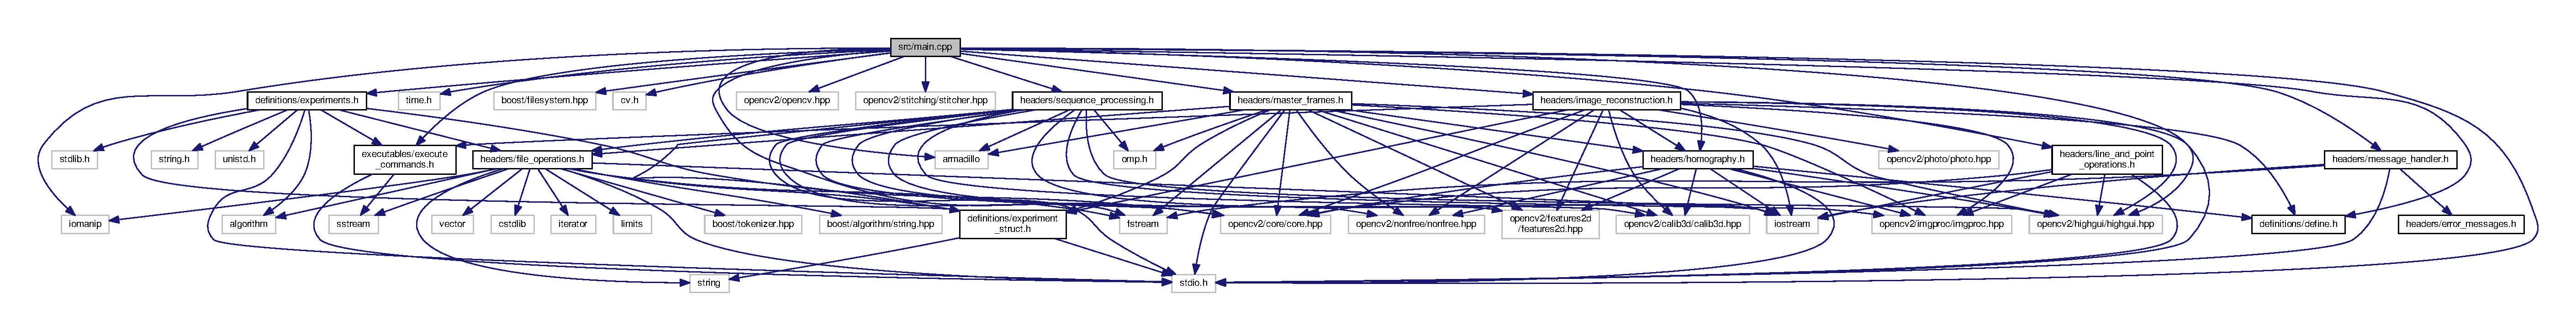
\includegraphics[width=350pt]{main_8cpp__incl}
\end{center}
\end{figure}
\subsection*{Functions}
\begin{DoxyCompactItemize}
\item 
std\+::string \hyperlink{main_8cpp_a96093b0a34cef38f0f27b7a636e637b0}{get\+It\+Formatted} (int frame\+\_\+number)
\begin{DoxyCompactList}\small\item\em get\+It\+Formatted -\/ Formats the number with padding. \end{DoxyCompactList}\item 
void \hyperlink{main_8cpp_aa20feaa0f15d8966a051a6e4754234ab}{write\+To\+Output} (cv\+::\+Video\+Writer \&save\+\_\+video, cv\+::\+Mat \&image, uint frame\+\_\+number)
\begin{DoxyCompactList}\small\item\em write\+To\+Output -\/ Writes the given image to the output (save\+\_\+video and/or screen) \end{DoxyCompactList}\item 
void \hyperlink{main_8cpp_ac701177e76d26612e87cbab9a0ee5218}{get\+Stable\+Frame\+Temporally} (cv\+::\+Mat \&input\+\_\+frame, cv\+::\+Mat \&homography\+\_\+matrix, const cv\+::\+Rect \&drop\+\_\+area, const cv\+::\+Rect \&crop\+\_\+area, int frame\+\_\+number, int d, int D, cv\+::vector$<$ int $>$ \&selected\+\_\+frames, const std\+::vector$<$ cv\+::\+Key\+Point $>$ \&keypoints\+\_\+master\+\_\+pre, const std\+::vector$<$ cv\+::\+Key\+Point $>$ \&keypoints\+\_\+master\+\_\+pos, const cv\+::\+Mat \&descriptors\+\_\+master\+\_\+pre, const cv\+::\+Mat \&descriptors\+\_\+master\+\_\+pos, int attempt, \hyperlink{classMessageHandler}{Message\+Handler} \&msg\+\_\+handler, cv\+::\+Mat \&stable\+\_\+frame)
\begin{DoxyCompactList}\small\item\em get\+Stable\+Frame -\/ Returns a frame stabilized given the parameters. \end{DoxyCompactList}\item 
void \hyperlink{main_8cpp_a12d6b6af5ae5297df5b19bb00f173df3}{get\+Stable\+Frame\+Spatially} (cv\+::\+Mat \&input\+\_\+frame, cv\+::\+Mat \&homography\+\_\+matrix, const cv\+::\+Rect \&drop\+\_\+area, const cv\+::\+Rect \&crop\+\_\+area, int frame\+\_\+number, float s, float S, cv\+::vector$<$ int $>$ \&selected\+\_\+frames, const std\+::vector$<$ cv\+::\+Key\+Point $>$ \&keypoints\+\_\+master\+\_\+pre, const std\+::vector$<$ cv\+::\+Key\+Point $>$ \&keypoints\+\_\+master\+\_\+pos, const cv\+::\+Mat \&descriptors\+\_\+master\+\_\+pre, const cv\+::\+Mat \&descriptors\+\_\+master\+\_\+pos, int attempt, \hyperlink{classMessageHandler}{Message\+Handler} \&msg\+\_\+handler, cv\+::\+Mat \&stable\+\_\+frame)
\begin{DoxyCompactList}\small\item\em get\+Stable\+Frame\+Temporally -\/ Returns a frame stabilized given the parameters. \end{DoxyCompactList}\item 
const std\+::string \hyperlink{main_8cpp_aa46369f3c8adbff876c82270346fffa2}{current\+Date\+Time} ()
\item 
int \hyperlink{main_8cpp_a0ddf1224851353fc92bfbff6f499fa97}{main} (int argc, char $\ast$argv\mbox{[}$\,$\mbox{]})
\begin{DoxyCompactList}\small\item\em \hyperlink{main_8cpp}{main.\+cpp} \end{DoxyCompactList}\end{DoxyCompactItemize}
\subsection*{Variables}
\begin{DoxyCompactItemize}
\item 
int \hyperlink{main_8cpp_a6725a70b6f47b0c88de524c592b70856}{log\+\_\+number\+\_\+length}
\item 
int \hyperlink{main_8cpp_a856a15ce171c3df67abaecb8cee8b78e}{num\+\_\+of\+\_\+reconstructed\+\_\+frames} = 0
\item 
int \hyperlink{main_8cpp_a40076974a0da2dbd3504b79979865d26}{num\+\_\+of\+\_\+dropped\+\_\+frames} = 0
\item 
int \hyperlink{main_8cpp_a2daaa9229b3fb806f774d4bcd6a08af5}{num\+\_\+of\+\_\+good\+\_\+frames} = 0
\item 
int \hyperlink{main_8cpp_a99a2ec99e6407a223577226b9715b73b}{num\+\_\+of\+\_\+fails\+\_\+in\+\_\+homography} = 0
\item 
int \hyperlink{main_8cpp_aad35f04e5303062bc8efbfdcc53cd604}{saved\+\_\+frames} = 0
\item 
\hyperlink{structEXPERIMENT}{E\+X\+P\+E\+R\+I\+M\+E\+NT} \hyperlink{main_8cpp_a9f5a81402e170475690f371d55cbe623}{experiment\+\_\+settings}
\end{DoxyCompactItemize}


\subsection{Detailed Description}
Main file that contains the \hyperlink{main_8cpp}{main.\+cpp}. 



\subsection{Function Documentation}
\index{main.\+cpp@{main.\+cpp}!current\+Date\+Time@{current\+Date\+Time}}
\index{current\+Date\+Time@{current\+Date\+Time}!main.\+cpp@{main.\+cpp}}
\subsubsection[{\texorpdfstring{current\+Date\+Time()}{currentDateTime()}}]{\setlength{\rightskip}{0pt plus 5cm}const std\+::string current\+Date\+Time (
\begin{DoxyParamCaption}
{}
\end{DoxyParamCaption}
)}\hypertarget{main_8cpp_aa46369f3c8adbff876c82270346fffa2}{}\label{main_8cpp_aa46369f3c8adbff876c82270346fffa2}
\index{main.\+cpp@{main.\+cpp}!get\+It\+Formatted@{get\+It\+Formatted}}
\index{get\+It\+Formatted@{get\+It\+Formatted}!main.\+cpp@{main.\+cpp}}
\subsubsection[{\texorpdfstring{get\+It\+Formatted(int frame\+\_\+number)}{getItFormatted(int frame\_number)}}]{\setlength{\rightskip}{0pt plus 5cm}std\+::string get\+It\+Formatted (
\begin{DoxyParamCaption}
\item[{int}]{frame\+\_\+number}
\end{DoxyParamCaption}
)}\hypertarget{main_8cpp_a96093b0a34cef38f0f27b7a636e637b0}{}\label{main_8cpp_a96093b0a34cef38f0f27b7a636e637b0}


get\+It\+Formatted -\/ Formats the number with padding. 


\begin{DoxyParams}{Parameters}
{\em frame\+\_\+number} & \\
\hline
\end{DoxyParams}
\begin{DoxyReturn}{Returns}

\end{DoxyReturn}
\begin{DoxyAuthor}{Author}
Washington Luis de Souza Ramos 
\end{DoxyAuthor}
\begin{DoxyDate}{Date}
10/09/2016 
\end{DoxyDate}
\index{main.\+cpp@{main.\+cpp}!get\+Stable\+Frame\+Spatially@{get\+Stable\+Frame\+Spatially}}
\index{get\+Stable\+Frame\+Spatially@{get\+Stable\+Frame\+Spatially}!main.\+cpp@{main.\+cpp}}
\subsubsection[{\texorpdfstring{get\+Stable\+Frame\+Spatially(cv\+::\+Mat \&input\+\_\+frame, cv\+::\+Mat \&homography\+\_\+matrix, const cv\+::\+Rect \&drop\+\_\+area, const cv\+::\+Rect \&crop\+\_\+area, int frame\+\_\+number, float s, float S, cv\+::vector$<$ int $>$ \&selected\+\_\+frames, const std\+::vector$<$ cv\+::\+Key\+Point $>$ \&keypoints\+\_\+master\+\_\+pre, const std\+::vector$<$ cv\+::\+Key\+Point $>$ \&keypoints\+\_\+master\+\_\+pos, const cv\+::\+Mat \&descriptors\+\_\+master\+\_\+pre, const cv\+::\+Mat \&descriptors\+\_\+master\+\_\+pos, int attempt, Message\+Handler \&msg\+\_\+handler, cv\+::\+Mat \&stable\+\_\+frame)}{getStableFrameSpatially(cv::Mat \&input\_frame, cv::Mat \&homography\_matrix, const cv::Rect \&drop\_area, const cv::Rect \&crop\_area, int frame\_number, float s, float S, cv::vector< int > \&selected\_frames, const std::vector< cv::KeyPoint > \&keypoints\_master\_pre, const std::vector< cv::KeyPoint > \&keypoints\_master\_pos, const cv::Mat \&descriptors\_master\_pre, const cv::Mat \&descriptors\_master\_pos, int attempt, MessageHandler \&msg\_handler, cv::Mat \&stable\_frame)}}]{\setlength{\rightskip}{0pt plus 5cm}void get\+Stable\+Frame\+Spatially (
\begin{DoxyParamCaption}
\item[{cv\+::\+Mat \&}]{input\+\_\+frame, }
\item[{cv\+::\+Mat \&}]{homography\+\_\+matrix, }
\item[{const cv\+::\+Rect \&}]{drop\+\_\+area, }
\item[{const cv\+::\+Rect \&}]{crop\+\_\+area, }
\item[{int}]{frame\+\_\+number, }
\item[{float}]{s, }
\item[{float}]{S, }
\item[{cv\+::vector$<$ int $>$ \&}]{selected\+\_\+frames, }
\item[{const std\+::vector$<$ cv\+::\+Key\+Point $>$ \&}]{keypoints\+\_\+master\+\_\+pre, }
\item[{const std\+::vector$<$ cv\+::\+Key\+Point $>$ \&}]{keypoints\+\_\+master\+\_\+pos, }
\item[{const cv\+::\+Mat \&}]{descriptors\+\_\+master\+\_\+pre, }
\item[{const cv\+::\+Mat \&}]{descriptors\+\_\+master\+\_\+pos, }
\item[{int}]{attempt, }
\item[{{\bf Message\+Handler} \&}]{msg\+\_\+handler, }
\item[{cv\+::\+Mat \&}]{stable\+\_\+frame}
\end{DoxyParamCaption}
)}\hypertarget{main_8cpp_a12d6b6af5ae5297df5b19bb00f173df3}{}\label{main_8cpp_a12d6b6af5ae5297df5b19bb00f173df3}


get\+Stable\+Frame\+Temporally -\/ Returns a frame stabilized given the parameters. 

get\+Stable\+Frame\+Spatially -\/ Returns a frame stabilized given the parameters.


\begin{DoxyParams}{Parameters}
{\em input\+\_\+frame} & \\
\hline
{\em homography\+\_\+matrix} & \\
\hline
{\em drop\+\_\+area} & \\
\hline
{\em crop\+\_\+area} & \\
\hline
{\em frame\+\_\+number} & \\
\hline
{\em s} & -\/ Spatial distance to the previous master (using the instability costs) \\
\hline
{\em S} & -\/ Spatial distance between the masters (using the instability costs) \\
\hline
{\em selected\+\_\+frames} & \\
\hline
{\em image\+\_\+master\+\_\+pre} & \\
\hline
{\em image\+\_\+master\+\_\+pos} & \\
\hline
{\em trial} & -\/ The number of the current attempt \\
\hline
{\em msg\+\_\+handler} & -\/ The message handler \\
\hline
{\em stable\+\_\+frame} & \\
\hline
\end{DoxyParams}
\begin{DoxyAuthor}{Author}
Washington Luis de Souza Ramos 
\end{DoxyAuthor}
\begin{DoxyDate}{Date}
10/09/2016 
\end{DoxyDate}
C\+A\+SE 1\+: Homography makes it good, frame is kept.

C\+A\+SE 2\+: Homography makes it regular, frame needs to be reconstructed

C\+A\+SE 2.\+1\+: Homography makes it awful, a new frame needs to be selected

C\+A\+SE 3\+: Homography makes it awful, a new frame needs to be selected \index{main.\+cpp@{main.\+cpp}!get\+Stable\+Frame\+Temporally@{get\+Stable\+Frame\+Temporally}}
\index{get\+Stable\+Frame\+Temporally@{get\+Stable\+Frame\+Temporally}!main.\+cpp@{main.\+cpp}}
\subsubsection[{\texorpdfstring{get\+Stable\+Frame\+Temporally(cv\+::\+Mat \&input\+\_\+frame, cv\+::\+Mat \&homography\+\_\+matrix, const cv\+::\+Rect \&drop\+\_\+area, const cv\+::\+Rect \&crop\+\_\+area, int frame\+\_\+number, int d, int D, cv\+::vector$<$ int $>$ \&selected\+\_\+frames, const std\+::vector$<$ cv\+::\+Key\+Point $>$ \&keypoints\+\_\+master\+\_\+pre, const std\+::vector$<$ cv\+::\+Key\+Point $>$ \&keypoints\+\_\+master\+\_\+pos, const cv\+::\+Mat \&descriptors\+\_\+master\+\_\+pre, const cv\+::\+Mat \&descriptors\+\_\+master\+\_\+pos, int attempt, Message\+Handler \&msg\+\_\+handler, cv\+::\+Mat \&stable\+\_\+frame)}{getStableFrameTemporally(cv::Mat \&input\_frame, cv::Mat \&homography\_matrix, const cv::Rect \&drop\_area, const cv::Rect \&crop\_area, int frame\_number, int d, int D, cv::vector< int > \&selected\_frames, const std::vector< cv::KeyPoint > \&keypoints\_master\_pre, const std::vector< cv::KeyPoint > \&keypoints\_master\_pos, const cv::Mat \&descriptors\_master\_pre, const cv::Mat \&descriptors\_master\_pos, int attempt, MessageHandler \&msg\_handler, cv::Mat \&stable\_frame)}}]{\setlength{\rightskip}{0pt plus 5cm}void get\+Stable\+Frame\+Temporally (
\begin{DoxyParamCaption}
\item[{cv\+::\+Mat \&}]{input\+\_\+frame, }
\item[{cv\+::\+Mat \&}]{homography\+\_\+matrix, }
\item[{const cv\+::\+Rect \&}]{drop\+\_\+area, }
\item[{const cv\+::\+Rect \&}]{crop\+\_\+area, }
\item[{int}]{frame\+\_\+number, }
\item[{int}]{d, }
\item[{int}]{D, }
\item[{cv\+::vector$<$ int $>$ \&}]{selected\+\_\+frames, }
\item[{const std\+::vector$<$ cv\+::\+Key\+Point $>$ \&}]{keypoints\+\_\+master\+\_\+pre, }
\item[{const std\+::vector$<$ cv\+::\+Key\+Point $>$ \&}]{keypoints\+\_\+master\+\_\+pos, }
\item[{const cv\+::\+Mat \&}]{descriptors\+\_\+master\+\_\+pre, }
\item[{const cv\+::\+Mat \&}]{descriptors\+\_\+master\+\_\+pos, }
\item[{int}]{attempt, }
\item[{{\bf Message\+Handler} \&}]{msg\+\_\+handler, }
\item[{cv\+::\+Mat \&}]{stable\+\_\+frame}
\end{DoxyParamCaption}
)}\hypertarget{main_8cpp_ac701177e76d26612e87cbab9a0ee5218}{}\label{main_8cpp_ac701177e76d26612e87cbab9a0ee5218}


get\+Stable\+Frame -\/ Returns a frame stabilized given the parameters. 

get\+Stable\+Frame\+Temporally -\/ Returns a frame stabilized given the parameters.


\begin{DoxyParams}{Parameters}
{\em input\+\_\+frame} & \\
\hline
{\em homography\+\_\+matrix} & \\
\hline
{\em drop\+\_\+area} & \\
\hline
{\em crop\+\_\+area} & \\
\hline
{\em frame\+\_\+number} & \\
\hline
{\em d} & \\
\hline
{\em D} & \\
\hline
{\em selected\+\_\+frames} & \\
\hline
{\em image\+\_\+master\+\_\+pre} & \\
\hline
{\em image\+\_\+master\+\_\+pos} & \\
\hline
{\em trial} & -\/ The number of the current attempt \\
\hline
{\em stable\+\_\+frame} & \\
\hline
\end{DoxyParams}
\begin{DoxyAuthor}{Author}
Washington Luis de Souza Ramos 
\end{DoxyAuthor}
\begin{DoxyDate}{Date}
10/09/2016
\end{DoxyDate}

\begin{DoxyParams}{Parameters}
{\em input\+\_\+frame} & \\
\hline
{\em homography\+\_\+matrix} & \\
\hline
{\em drop\+\_\+area} & \\
\hline
{\em crop\+\_\+area} & \\
\hline
{\em frame\+\_\+number} & \\
\hline
{\em d} & -\/ Temporal distance to the previous master \\
\hline
{\em D} & -\/ Temporal distance between the masters \\
\hline
{\em selected\+\_\+frames} & \\
\hline
{\em image\+\_\+master\+\_\+pre} & \\
\hline
{\em image\+\_\+master\+\_\+pos} & \\
\hline
{\em trial} & -\/ The number of the current attempt \\
\hline
{\em msg\+\_\+handler} & -\/ The message handler \\
\hline
{\em stable\+\_\+frame} & \\
\hline
\end{DoxyParams}
\begin{DoxyAuthor}{Author}
Washington Luis de Souza Ramos 
\end{DoxyAuthor}
\begin{DoxyDate}{Date}
10/09/2016 
\end{DoxyDate}
C\+A\+SE 1\+: Homography makes it good, frame is kept.

C\+A\+SE 2\+: Homography makes it regular, frame needs to be reconstructed

C\+A\+SE 2.\+1\+: Homography makes it awful, a new frame needs to be selected

C\+A\+SE 3\+: Homography makes it awful, a new frame needs to be selected \index{main.\+cpp@{main.\+cpp}!main@{main}}
\index{main@{main}!main.\+cpp@{main.\+cpp}}
\subsubsection[{\texorpdfstring{main(int argc, char $\ast$argv[])}{main(int argc, char *argv[])}}]{\setlength{\rightskip}{0pt plus 5cm}int main (
\begin{DoxyParamCaption}
\item[{int}]{argc, }
\item[{char $\ast$}]{argv\mbox{[}$\,$\mbox{]}}
\end{DoxyParamCaption}
)}\hypertarget{main_8cpp_a0ddf1224851353fc92bfbff6f499fa97}{}\label{main_8cpp_a0ddf1224851353fc92bfbff6f499fa97}


\hyperlink{main_8cpp}{main.\+cpp} 

{\bfseries Usage\+:} ~\newline
$<$ Program\+\_\+name $>$ $<$ Settings\+\_\+file $>$ \mbox{[} Range\+\_\+min = 0 \mbox{]} \mbox{[} Range\+\_\+max = num\+\_\+frames \mbox{]} ~\newline
~\newline
Example 1\+: Run Video\+Stabilization in the Experiment\+\_\+1 processing the whole video. ~\newline
-\/$>$ Video\+Stabilization Experiment\+\_\+1.\+xml ~\newline
Example 2\+: Run Video\+Stabilization in the Experiment\+\_\+1 processing from the 150 frame until the last one. ~\newline
-\/$>$ Video\+Stabilization Experiment\+\_\+1.\+xml 150 ~\newline
Example 2\+: Run Video\+Stabilization in the Experiment\+\_\+1 processing from the 150 frame until the frame 490. ~\newline
-\/$>$ Video\+Stabilization Experiment\+\_\+1.\+xml 150 490 ~\newline
~\newline
 The program can {\bfseries exit} with following codes\+: ~\newline
{\bfseries -\/1} -\/ Wrong number of input parameters. ~\newline
{\bfseries -\/2} -\/ Experiment id does not exist. ~\newline
{\bfseries -\/3} -\/ Can not open the accelerated video. ~\newline
{\bfseries -\/4} -\/ Can not create file to save the output video. ~\newline
{\bfseries -\/5} -\/ Can not open the video original video. ~\newline
{\bfseries -\/6} -\/ Can not open the C\+SV file with the selected frame numbers of the accelerated video. ~\newline
{\bfseries -\/7} -\/ Can not create directory to save the output data. ~\newline
{\bfseries -\/8} -\/ Can not create log text file. ~\newline
{\bfseries -\/9} -\/ Range limits is not well defined. ~\newline
{\bfseries -\/10} -\/ Can not open the C\+SV file with the semantic costs of the original video. ~\newline
{\bfseries -\/11} -\/ transition from frame\+\_\+src to frame\+\_\+dst larger than number of transitions describle int the file the semantic costs


\begin{DoxyParams}{Parameters}
{\em argc} & -\/ number of parameters in argv. \\
\hline
{\em argv} & -\/ $<$ Settings\+\_\+file $>$ \mbox{[} Range\+\_\+min = 0 \mbox{]} \mbox{[} Range\+\_\+max = num\+\_\+frames \mbox{]} \\
\hline
\end{DoxyParams}
W\+R\+I\+T\+I\+NG T\+HE R\+E\+S\+U\+LT TO T\+HE O\+U\+T\+P\+UT ///

W\+R\+I\+T\+I\+NG T\+HE R\+E\+S\+U\+LT TO T\+HE O\+U\+T\+P\+UT ///

T\+H\+IS IS N\+OT A M\+A\+S\+T\+ER F\+R\+A\+ME ///

T\+H\+IS IS A M\+A\+S\+T\+ER F\+R\+A\+ME ///

W\+R\+I\+T\+I\+NG T\+HE R\+E\+S\+U\+LT TO T\+HE O\+U\+T\+P\+UT ///

W\+R\+I\+T\+I\+NG T\+HE R\+E\+S\+U\+LT TO T\+HE O\+U\+T\+P\+UT ///

W\+R\+I\+T\+I\+NG T\+HE R\+E\+S\+U\+LT TO T\+HE O\+U\+T\+P\+UT ///\index{main.\+cpp@{main.\+cpp}!write\+To\+Output@{write\+To\+Output}}
\index{write\+To\+Output@{write\+To\+Output}!main.\+cpp@{main.\+cpp}}
\subsubsection[{\texorpdfstring{write\+To\+Output(cv\+::\+Video\+Writer \&save\+\_\+video, cv\+::\+Mat \&image, uint frame\+\_\+number)}{writeToOutput(cv::VideoWriter \&save\_video, cv::Mat \&image, uint frame\_number)}}]{\setlength{\rightskip}{0pt plus 5cm}void write\+To\+Output (
\begin{DoxyParamCaption}
\item[{cv\+::\+Video\+Writer \&}]{save\+\_\+video, }
\item[{cv\+::\+Mat \&}]{image, }
\item[{uint}]{frame\+\_\+number}
\end{DoxyParamCaption}
)}\hypertarget{main_8cpp_aa20feaa0f15d8966a051a6e4754234ab}{}\label{main_8cpp_aa20feaa0f15d8966a051a6e4754234ab}


write\+To\+Output -\/ Writes the given image to the output (save\+\_\+video and/or screen) 


\begin{DoxyParams}{Parameters}
{\em save\+\_\+video} & \\
\hline
{\em image} & \\
\hline
{\em frame\+\_\+number} & \\
\hline
\end{DoxyParams}
\begin{DoxyAuthor}{Author}
Washington Luis de Souza Ramos 
\end{DoxyAuthor}
\begin{DoxyDate}{Date}
10/09/2016 
\end{DoxyDate}


\subsection{Variable Documentation}
\index{main.\+cpp@{main.\+cpp}!experiment\+\_\+settings@{experiment\+\_\+settings}}
\index{experiment\+\_\+settings@{experiment\+\_\+settings}!main.\+cpp@{main.\+cpp}}
\subsubsection[{\texorpdfstring{experiment\+\_\+settings}{experiment\_settings}}]{\setlength{\rightskip}{0pt plus 5cm}{\bf E\+X\+P\+E\+R\+I\+M\+E\+NT} experiment\+\_\+settings}\hypertarget{main_8cpp_a9f5a81402e170475690f371d55cbe623}{}\label{main_8cpp_a9f5a81402e170475690f371d55cbe623}
\index{main.\+cpp@{main.\+cpp}!log\+\_\+number\+\_\+length@{log\+\_\+number\+\_\+length}}
\index{log\+\_\+number\+\_\+length@{log\+\_\+number\+\_\+length}!main.\+cpp@{main.\+cpp}}
\subsubsection[{\texorpdfstring{log\+\_\+number\+\_\+length}{log\_number\_length}}]{\setlength{\rightskip}{0pt plus 5cm}int log\+\_\+number\+\_\+length}\hypertarget{main_8cpp_a6725a70b6f47b0c88de524c592b70856}{}\label{main_8cpp_a6725a70b6f47b0c88de524c592b70856}
\index{main.\+cpp@{main.\+cpp}!num\+\_\+of\+\_\+dropped\+\_\+frames@{num\+\_\+of\+\_\+dropped\+\_\+frames}}
\index{num\+\_\+of\+\_\+dropped\+\_\+frames@{num\+\_\+of\+\_\+dropped\+\_\+frames}!main.\+cpp@{main.\+cpp}}
\subsubsection[{\texorpdfstring{num\+\_\+of\+\_\+dropped\+\_\+frames}{num\_of\_dropped\_frames}}]{\setlength{\rightskip}{0pt plus 5cm}int num\+\_\+of\+\_\+dropped\+\_\+frames = 0}\hypertarget{main_8cpp_a40076974a0da2dbd3504b79979865d26}{}\label{main_8cpp_a40076974a0da2dbd3504b79979865d26}
\index{main.\+cpp@{main.\+cpp}!num\+\_\+of\+\_\+fails\+\_\+in\+\_\+homography@{num\+\_\+of\+\_\+fails\+\_\+in\+\_\+homography}}
\index{num\+\_\+of\+\_\+fails\+\_\+in\+\_\+homography@{num\+\_\+of\+\_\+fails\+\_\+in\+\_\+homography}!main.\+cpp@{main.\+cpp}}
\subsubsection[{\texorpdfstring{num\+\_\+of\+\_\+fails\+\_\+in\+\_\+homography}{num\_of\_fails\_in\_homography}}]{\setlength{\rightskip}{0pt plus 5cm}int num\+\_\+of\+\_\+fails\+\_\+in\+\_\+homography = 0}\hypertarget{main_8cpp_a99a2ec99e6407a223577226b9715b73b}{}\label{main_8cpp_a99a2ec99e6407a223577226b9715b73b}
\index{main.\+cpp@{main.\+cpp}!num\+\_\+of\+\_\+good\+\_\+frames@{num\+\_\+of\+\_\+good\+\_\+frames}}
\index{num\+\_\+of\+\_\+good\+\_\+frames@{num\+\_\+of\+\_\+good\+\_\+frames}!main.\+cpp@{main.\+cpp}}
\subsubsection[{\texorpdfstring{num\+\_\+of\+\_\+good\+\_\+frames}{num\_of\_good\_frames}}]{\setlength{\rightskip}{0pt plus 5cm}int num\+\_\+of\+\_\+good\+\_\+frames = 0}\hypertarget{main_8cpp_a2daaa9229b3fb806f774d4bcd6a08af5}{}\label{main_8cpp_a2daaa9229b3fb806f774d4bcd6a08af5}
\index{main.\+cpp@{main.\+cpp}!num\+\_\+of\+\_\+reconstructed\+\_\+frames@{num\+\_\+of\+\_\+reconstructed\+\_\+frames}}
\index{num\+\_\+of\+\_\+reconstructed\+\_\+frames@{num\+\_\+of\+\_\+reconstructed\+\_\+frames}!main.\+cpp@{main.\+cpp}}
\subsubsection[{\texorpdfstring{num\+\_\+of\+\_\+reconstructed\+\_\+frames}{num\_of\_reconstructed\_frames}}]{\setlength{\rightskip}{0pt plus 5cm}int num\+\_\+of\+\_\+reconstructed\+\_\+frames = 0}\hypertarget{main_8cpp_a856a15ce171c3df67abaecb8cee8b78e}{}\label{main_8cpp_a856a15ce171c3df67abaecb8cee8b78e}
\index{main.\+cpp@{main.\+cpp}!saved\+\_\+frames@{saved\+\_\+frames}}
\index{saved\+\_\+frames@{saved\+\_\+frames}!main.\+cpp@{main.\+cpp}}
\subsubsection[{\texorpdfstring{saved\+\_\+frames}{saved\_frames}}]{\setlength{\rightskip}{0pt plus 5cm}int saved\+\_\+frames = 0}\hypertarget{main_8cpp_aad35f04e5303062bc8efbfdcc53cd604}{}\label{main_8cpp_aad35f04e5303062bc8efbfdcc53cd604}

\hypertarget{master__frames_8cpp}{}\section{src/master\+\_\+frames.cpp File Reference}
\label{master__frames_8cpp}\index{src/master\+\_\+frames.\+cpp@{src/master\+\_\+frames.\+cpp}}


Functions to get the master frames from file or calculating it.  


{\ttfamily \#include \char`\"{}executables/execute\+\_\+commands.\+h\char`\"{}}\\*
{\ttfamily \#include \char`\"{}headers/master\+\_\+frames.\+h\char`\"{}}\\*
Include dependency graph for master\+\_\+frames.\+cpp\+:\nopagebreak
\begin{figure}[H]
\begin{center}
\leavevmode
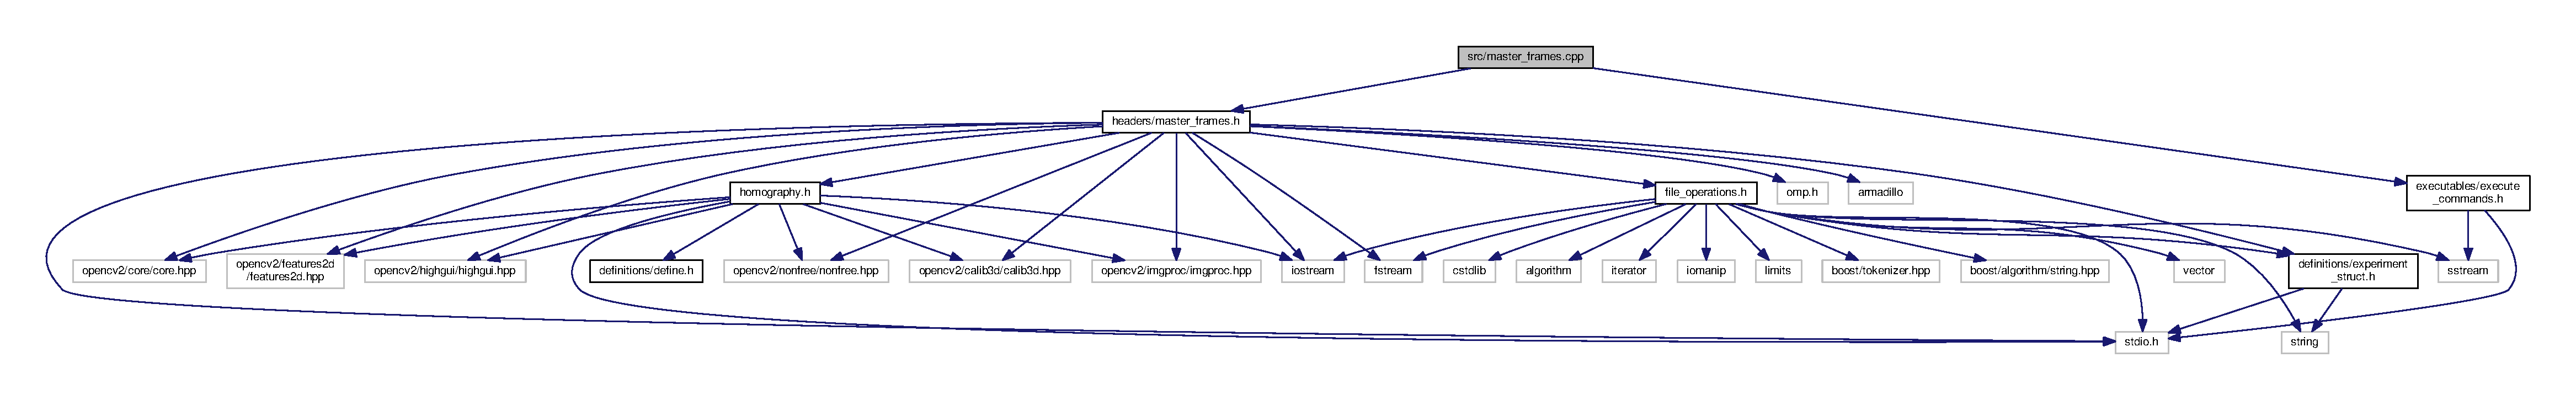
\includegraphics[width=350pt]{master__frames_8cpp__incl}
\end{center}
\end{figure}
\subsection*{Functions}
\begin{DoxyCompactItemize}
\item 
int \hyperlink{master__frames_8cpp_add63ac6145fd4d298e34df91185136b1}{length} (int number)
\begin{DoxyCompactList}\small\item\em Function that counts the digits of the number. \end{DoxyCompactList}\item 
std\+::vector$<$ int $>$ \hyperlink{master__frames_8cpp_a28e2c72651b4fe01415691078fd3061c}{find\+Master\+Frames} (const \hyperlink{structEXPERIMENT}{E\+X\+P\+E\+R\+I\+M\+E\+NT} \&\hyperlink{main_8cpp_a9f5a81402e170475690f371d55cbe623}{experiment\+\_\+settings})
\begin{DoxyCompactList}\small\item\em Function that calculates the master frames in a sequence given a N in the field segment\+Size in the experiment\+\_\+settings in a non-\/parallel (sequential) way. \end{DoxyCompactList}\item 
std\+::vector$<$ int $>$ \hyperlink{master__frames_8cpp_a30ead0e7bdbe71513f65101a29913d70}{find\+Master\+Frames\+Parallel} (const \hyperlink{structEXPERIMENT}{E\+X\+P\+E\+R\+I\+M\+E\+NT} \&\hyperlink{main_8cpp_a9f5a81402e170475690f371d55cbe623}{experiment\+\_\+settings})
\begin{DoxyCompactList}\small\item\em Function that calculates the master frames in a sequence given a N in the field segment\+Size in the experiment\+\_\+settings in a parallel way. \end{DoxyCompactList}\item 
std\+::vector$<$ int $>$ \hyperlink{master__frames_8cpp_af399de8fc7e31d60cccdf90efa80541c}{get\+Master\+Frames} (const \hyperlink{structEXPERIMENT}{E\+X\+P\+E\+R\+I\+M\+E\+NT} \hyperlink{main_8cpp_a9f5a81402e170475690f371d55cbe623}{experiment\+\_\+settings}, const int num\+\_\+frames)
\begin{DoxyCompactList}\small\item\em Function that return the master frames in a sequence according with experiment settings, by load from a file or calculating them. \end{DoxyCompactList}\end{DoxyCompactItemize}


\subsection{Detailed Description}
Functions to get the master frames from file or calculating it. 

Calculate master frames. Calculate master frames in a parallel way. Call \hyperlink{file__operations_8cpp}{file\+\_\+operations.\+cpp} methods to get read master frames from file. 

\subsection{Function Documentation}
\index{master\+\_\+frames.\+cpp@{master\+\_\+frames.\+cpp}!find\+Master\+Frames@{find\+Master\+Frames}}
\index{find\+Master\+Frames@{find\+Master\+Frames}!master\+\_\+frames.\+cpp@{master\+\_\+frames.\+cpp}}
\subsubsection[{\texorpdfstring{find\+Master\+Frames(const E\+X\+P\+E\+R\+I\+M\+E\+N\+T \&experiment\+\_\+settings)}{findMasterFrames(const EXPERIMENT \&experiment\_settings)}}]{\setlength{\rightskip}{0pt plus 5cm}std\+::vector$<$int$>$ find\+Master\+Frames (
\begin{DoxyParamCaption}
\item[{const {\bf E\+X\+P\+E\+R\+I\+M\+E\+NT} \&}]{experiment\+\_\+settings}
\end{DoxyParamCaption}
)}\hypertarget{master__frames_8cpp_a28e2c72651b4fe01415691078fd3061c}{}\label{master__frames_8cpp_a28e2c72651b4fe01415691078fd3061c}


Function that calculates the master frames in a sequence given a N in the field segment\+Size in the experiment\+\_\+settings in a non-\/parallel (sequential) way. 


\begin{DoxyParams}{Parameters}
{\em experiment\+\_\+settings} & -\/ object with the experiment settings.\\
\hline
\end{DoxyParams}
\begin{DoxyReturn}{Returns}
{\ttfamily std\+::vector$<$int$>$} -\/ vector with the master frames found in the sequence.
\end{DoxyReturn}
\begin{DoxyAuthor}{Author}
Michel Melo da Silva 
\end{DoxyAuthor}
\begin{DoxyDate}{Date}
02/04/2016 
\end{DoxyDate}
\index{master\+\_\+frames.\+cpp@{master\+\_\+frames.\+cpp}!find\+Master\+Frames\+Parallel@{find\+Master\+Frames\+Parallel}}
\index{find\+Master\+Frames\+Parallel@{find\+Master\+Frames\+Parallel}!master\+\_\+frames.\+cpp@{master\+\_\+frames.\+cpp}}
\subsubsection[{\texorpdfstring{find\+Master\+Frames\+Parallel(const E\+X\+P\+E\+R\+I\+M\+E\+N\+T \&experiment\+\_\+settings)}{findMasterFramesParallel(const EXPERIMENT \&experiment\_settings)}}]{\setlength{\rightskip}{0pt plus 5cm}std\+::vector$<$int$>$ find\+Master\+Frames\+Parallel (
\begin{DoxyParamCaption}
\item[{const {\bf E\+X\+P\+E\+R\+I\+M\+E\+NT} \&}]{experiment\+\_\+settings}
\end{DoxyParamCaption}
)}\hypertarget{master__frames_8cpp_a30ead0e7bdbe71513f65101a29913d70}{}\label{master__frames_8cpp_a30ead0e7bdbe71513f65101a29913d70}


Function that calculates the master frames in a sequence given a N in the field segment\+Size in the experiment\+\_\+settings in a parallel way. 


\begin{DoxyParams}{Parameters}
{\em experiment\+\_\+settings} & -\/ object with the experiment settings.\\
\hline
\end{DoxyParams}
\begin{DoxyReturn}{Returns}
{\ttfamily std\+::vector$<$int$>$} -\/ vector with the master frames found in the sequence.
\end{DoxyReturn}
\begin{DoxyAuthor}{Author}
Michel Melo da Silva 
\end{DoxyAuthor}
\begin{DoxyDate}{Date}
03/04/2016 
\end{DoxyDate}
\index{master\+\_\+frames.\+cpp@{master\+\_\+frames.\+cpp}!get\+Master\+Frames@{get\+Master\+Frames}}
\index{get\+Master\+Frames@{get\+Master\+Frames}!master\+\_\+frames.\+cpp@{master\+\_\+frames.\+cpp}}
\subsubsection[{\texorpdfstring{get\+Master\+Frames(const E\+X\+P\+E\+R\+I\+M\+E\+N\+T experiment\+\_\+settings, const int num\+\_\+frames)}{getMasterFrames(const EXPERIMENT experiment\_settings, const int num\_frames)}}]{\setlength{\rightskip}{0pt plus 5cm}std\+::vector$<$int$>$ get\+Master\+Frames (
\begin{DoxyParamCaption}
\item[{const {\bf E\+X\+P\+E\+R\+I\+M\+E\+NT}}]{experiment\+\_\+settings, }
\item[{const int}]{num\+\_\+frames}
\end{DoxyParamCaption}
)}\hypertarget{master__frames_8cpp_af399de8fc7e31d60cccdf90efa80541c}{}\label{master__frames_8cpp_af399de8fc7e31d60cccdf90efa80541c}


Function that return the master frames in a sequence according with experiment settings, by load from a file or calculating them. 


\begin{DoxyParams}{Parameters}
{\em experiment\+\_\+settings} & -\/ object with the experiment settings. \\
\hline
{\em num\+\_\+frames} & -\/ number of frames of the reduced video.\\
\hline
\end{DoxyParams}
\begin{DoxyReturn}{Returns}
{\ttfamily std\+::vector$<$int$>$} -\/ vector with the master frames found in the sequence.
\end{DoxyReturn}
\begin{DoxyAuthor}{Author}
Michel Melo da Silva 
\end{DoxyAuthor}
\begin{DoxyDate}{Date}
04/04/2016 
\end{DoxyDate}
\index{master\+\_\+frames.\+cpp@{master\+\_\+frames.\+cpp}!length@{length}}
\index{length@{length}!master\+\_\+frames.\+cpp@{master\+\_\+frames.\+cpp}}
\subsubsection[{\texorpdfstring{length(int number)}{length(int number)}}]{\setlength{\rightskip}{0pt plus 5cm}int length (
\begin{DoxyParamCaption}
\item[{int}]{number}
\end{DoxyParamCaption}
)}\hypertarget{master__frames_8cpp_add63ac6145fd4d298e34df91185136b1}{}\label{master__frames_8cpp_add63ac6145fd4d298e34df91185136b1}


Function that counts the digits of the number. 


\begin{DoxyParams}{Parameters}
{\em number} & -\/ number to calculate the number of digits.\\
\hline
\end{DoxyParams}
\begin{DoxyReturn}{Returns}
{\ttfamily int} -\/ number of digits of the input number.
\end{DoxyReturn}
\begin{DoxyAuthor}{Author}
Michel Melo da Silva 
\end{DoxyAuthor}
\begin{DoxyDate}{Date}
20/04/2016 
\end{DoxyDate}

\hypertarget{message__handler_8cpp}{}\section{src/message\+\_\+handler.cpp File Reference}
\label{message__handler_8cpp}\index{src/message\+\_\+handler.\+cpp@{src/message\+\_\+handler.\+cpp}}
{\ttfamily \#include \char`\"{}headers/message\+\_\+handler.\+h\char`\"{}}\\*
{\ttfamily \#include \char`\"{}definitions/define.\+h\char`\"{}}\\*
Include dependency graph for message\+\_\+handler.\+cpp\+:\nopagebreak
\begin{figure}[H]
\begin{center}
\leavevmode
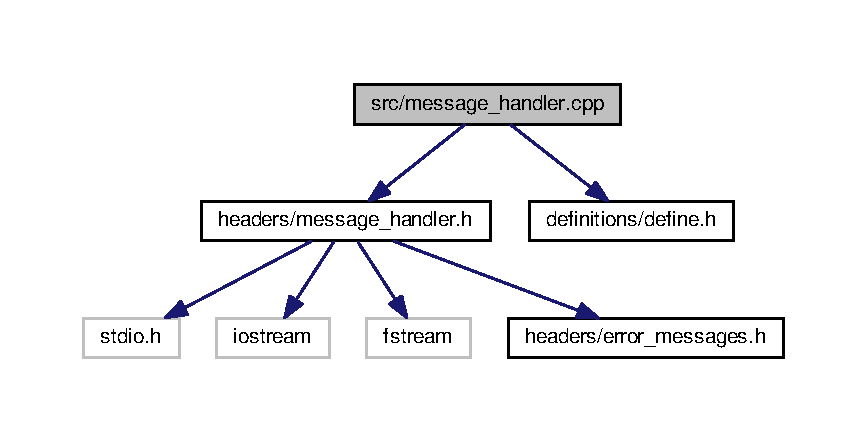
\includegraphics[width=350pt]{message__handler_8cpp__incl}
\end{center}
\end{figure}

\hypertarget{sequence__processing_8cpp}{}\section{src/sequence\+\_\+processing.cpp File Reference}
\label{sequence__processing_8cpp}\index{src/sequence\+\_\+processing.\+cpp@{src/sequence\+\_\+processing.\+cpp}}


Functions related with sequence processing, such as find intermediate homography, get transition weight, select new frame.  


{\ttfamily \#include \char`\"{}definitions/experiment\+\_\+struct.\+h\char`\"{}}\\*
{\ttfamily \#include \char`\"{}headers/sequence\+\_\+processing.\+h\char`\"{}}\\*
{\ttfamily \#include \char`\"{}headers/homography.\+h\char`\"{}}\\*
Include dependency graph for sequence\+\_\+processing.\+cpp\+:\nopagebreak
\begin{figure}[H]
\begin{center}
\leavevmode
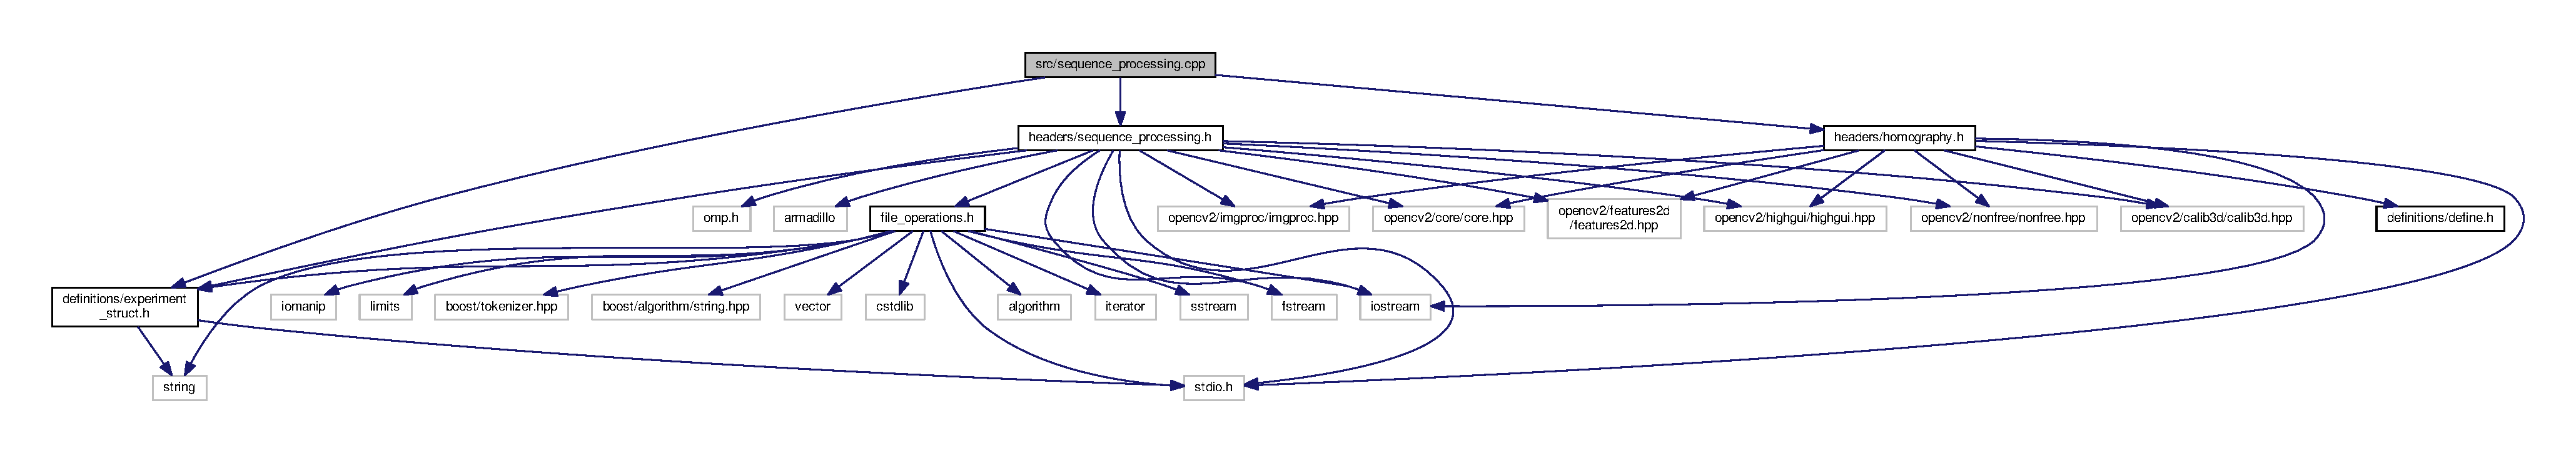
\includegraphics[width=350pt]{sequence__processing_8cpp__incl}
\end{center}
\end{figure}
\subsection*{Functions}
\begin{DoxyCompactItemize}
\item 
bool \hyperlink{sequence__processing_8cpp_a31c3927c6071e5c6543de6934dac2731}{matrix\+Root} (cv\+::\+Mat \&matrix, int root, cv\+::\+Mat \&matrix\+\_\+result)
\begin{DoxyCompactList}\small\item\em Function that calculates the n-\/ith root of a matrix. \end{DoxyCompactList}\item 
void \hyperlink{sequence__processing_8cpp_ad83b7c4de86f1a2ed3a79b37ea347890}{matrix\+Pow} (cv\+::\+Mat \&matrix, int pow, cv\+::\+Mat \&matrix\+\_\+result)
\begin{DoxyCompactList}\small\item\em Function that calculates the n-\/ith pow of a matrix. \end{DoxyCompactList}\item 
bool \hyperlink{sequence__processing_8cpp_aad08ac53f56a97ead9e9e2a4e167e4d8}{find\+Intermediate\+Homography\+Matrix} (const int d, const int D, const int N, const cv\+::\+Mat \&frame\+\_\+i, const cv\+::\+Mat \&frame\+\_\+master\+\_\+pre, const cv\+::\+Mat \&frame\+\_\+master\+\_\+pos, cv\+::\+Mat \&homography\+\_\+matrix\+\_\+result)
\begin{DoxyCompactList}\small\item\em Function that calculates the homography matrix that leave the frame\+\_\+i to the intermediate plan between the plans of frame\+\_\+master\+\_\+pre and frame\+\_\+master\+\_\+pre with relation of the distance between them. \end{DoxyCompactList}\item 
bool \hyperlink{sequence__processing_8cpp_a536d6b62274f62941d6cec32549d2543}{find\+Intermediate\+Homography\+Matrix} (const int d, const int D, const int N, const cv\+::\+Mat \&frame\+\_\+i, const std\+::vector$<$ cv\+::\+Key\+Point $>$ \&keypoints\+\_\+master\+\_\+pre, const std\+::vector$<$ cv\+::\+Key\+Point $>$ \&keypoints\+\_\+master\+\_\+pos, const cv\+::\+Mat \&descriptors\+\_\+master\+\_\+pre, const cv\+::\+Mat \&descriptors\+\_\+master\+\_\+pos, cv\+::\+Mat \&homography\+\_\+matrix\+\_\+result)
\begin{DoxyCompactList}\small\item\em Function that calculates the homography matrix that leave the frame\+\_\+i to the intermediate plan between the frames related to the previous and posterior master, with respect to the distance between them. \end{DoxyCompactList}\item 
bool \hyperlink{sequence__processing_8cpp_aa692e8a44dcab5dc3c45c35c3f7ae6d2}{find\+Intermediate\+Homography\+Matrix} (const float s, const float S, const cv\+::\+Mat \&frame\+\_\+i, const std\+::vector$<$ cv\+::\+Key\+Point $>$ \&keypoints\+\_\+master\+\_\+pre, const std\+::vector$<$ cv\+::\+Key\+Point $>$ \&keypoints\+\_\+master\+\_\+pos, const cv\+::\+Mat \&descriptors\+\_\+master\+\_\+pre, const cv\+::\+Mat \&descriptors\+\_\+master\+\_\+pos, cv\+::\+Mat \&homography\+\_\+matrix\+\_\+result)
\begin{DoxyCompactList}\small\item\em Function that calculates the homography matrix that leave the frame\+\_\+i to the intermediate plan between the frames related to the previous and posterior master, with respect to the distance between them. \end{DoxyCompactList}\item 
double \hyperlink{sequence__processing_8cpp_a23162fd5114a89b24c3c7da9abb3915b}{gaussian\+Value} (double index)
\begin{DoxyCompactList}\small\item\em Function that calculates Gaussian value in the position index. \end{DoxyCompactList}\item 
float \hyperlink{sequence__processing_8cpp_ab65613bc69028dc0a72f09caa37d37ee}{frame\+Weight} (const int ransac\+\_\+inliers\+\_\+previous, const int ransac\+\_\+inliers\+\_\+posterior, const double area\+\_\+ratio, const double \hyperlink{sequence__processing_8cpp_a8d56592b555a0cbab5ace1db16a3b29b}{semantic\+\_\+weight})
\begin{DoxyCompactList}\small\item\em Function that calculates the frame weigth used to chose a new frame to compose the video. \end{DoxyCompactList}\item 
double \hyperlink{sequence__processing_8cpp_a8d56592b555a0cbab5ace1db16a3b29b}{semantic\+\_\+weight} (const int index\+\_\+previous, const int index\+\_\+current, const int index\+\_\+posterior, const \hyperlink{structEXPERIMENT}{E\+X\+P\+E\+R\+I\+M\+E\+NT} \&\hyperlink{main_8cpp_a9f5a81402e170475690f371d55cbe623}{experiment\+\_\+settings})
\begin{DoxyCompactList}\small\item\em Function that get the semantic information of the transition from the frame\+\_\+src to the frame\+\_\+dst calculted by M\+A\+T\+L\+AB and saved in a C\+SV file. \end{DoxyCompactList}\item 
int \hyperlink{sequence__processing_8cpp_a8374c98e95b78cc5027c494103e35348}{select\+New\+Frame} (const int d, const int D, const int N, const int index, const int index\+\_\+previous, const int index\+\_\+posterior, const std\+::vector$<$ cv\+::\+Key\+Point $>$ \&keypoints\+\_\+master\+\_\+pre, const std\+::vector$<$ cv\+::\+Key\+Point $>$ \&keypoints\+\_\+master\+\_\+pos, const cv\+::\+Mat \&descriptors\+\_\+master\+\_\+pre, const cv\+::\+Mat \&descriptors\+\_\+master\+\_\+pos, const cv\+::\+Rect \&crop\+\_\+area, const \hyperlink{structEXPERIMENT}{E\+X\+P\+E\+R\+I\+M\+E\+NT} \&\hyperlink{main_8cpp_a9f5a81402e170475690f371d55cbe623}{experiment\+\_\+settings}, cv\+::\+Mat \&new\+\_\+frame)
\begin{DoxyCompactList}\small\item\em Function that selects a new frame in the original video using the values of semantic information of the transition from the frame\+\_\+src to the frame\+\_\+dst calculted by M\+A\+T\+L\+AB and saved in a C\+SV file, the area ratio of the iamge after apply the homography transformation and the R\+A\+N\+S\+C\+AC inliers from the previous and posterior frames that compose the reduced video. \end{DoxyCompactList}\item 
int \hyperlink{sequence__processing_8cpp_a029dc4caa330843be4ee108a5e7bb825}{select\+New\+Frame} (const float s, const float S, const int index, const int index\+\_\+previous, const int index\+\_\+posterior, const std\+::vector$<$ cv\+::\+Key\+Point $>$ \&keypoints\+\_\+master\+\_\+pre, const std\+::vector$<$ cv\+::\+Key\+Point $>$ \&keypoints\+\_\+master\+\_\+pos, const cv\+::\+Mat \&descriptors\+\_\+master\+\_\+pre, const cv\+::\+Mat \&descriptors\+\_\+master\+\_\+pos, const cv\+::\+Rect \&crop\+\_\+area, const \hyperlink{structEXPERIMENT}{E\+X\+P\+E\+R\+I\+M\+E\+NT} \&\hyperlink{main_8cpp_a9f5a81402e170475690f371d55cbe623}{experiment\+\_\+settings}, cv\+::\+Mat \&new\+\_\+frame)
\begin{DoxyCompactList}\small\item\em Function that selects a new frame in the original video using the values of semantic information of the transition from the frame\+\_\+src to the frame\+\_\+dst calculted by M\+A\+T\+L\+AB and saved in a C\+SV file, the area ratio of the iamge after apply the homography transformation and the R\+A\+N\+S\+C\+AC inliers from the previous and posterior frames that compose the reduced video. \end{DoxyCompactList}\end{DoxyCompactItemize}


\subsection{Detailed Description}
Functions related with sequence processing, such as find intermediate homography, get transition weight, select new frame. 

Calculate intermediate homography matrix. Calculate matrix operations root and pow. Calculate frame weight. Get transition weight. Select new frame from original video. 

\subsection{Function Documentation}
\index{sequence\+\_\+processing.\+cpp@{sequence\+\_\+processing.\+cpp}!find\+Intermediate\+Homography\+Matrix@{find\+Intermediate\+Homography\+Matrix}}
\index{find\+Intermediate\+Homography\+Matrix@{find\+Intermediate\+Homography\+Matrix}!sequence\+\_\+processing.\+cpp@{sequence\+\_\+processing.\+cpp}}
\subsubsection[{\texorpdfstring{find\+Intermediate\+Homography\+Matrix(const int d, const int D, const int N, const cv\+::\+Mat \&frame\+\_\+i, const cv\+::\+Mat \&frame\+\_\+master\+\_\+pre, const cv\+::\+Mat \&frame\+\_\+master\+\_\+pos, cv\+::\+Mat \&homography\+\_\+matrix\+\_\+result)}{findIntermediateHomographyMatrix(const int d, const int D, const int N, const cv::Mat \&frame\_i, const cv::Mat \&frame\_master\_pre, const cv::Mat \&frame\_master\_pos, cv::Mat \&homography\_matrix\_result)}}]{\setlength{\rightskip}{0pt plus 5cm}bool find\+Intermediate\+Homography\+Matrix (
\begin{DoxyParamCaption}
\item[{const int}]{d, }
\item[{const int}]{D, }
\item[{const int}]{N, }
\item[{const cv\+::\+Mat \&}]{frame\+\_\+i, }
\item[{const cv\+::\+Mat \&}]{frame\+\_\+master\+\_\+pre, }
\item[{const cv\+::\+Mat \&}]{frame\+\_\+master\+\_\+pos, }
\item[{cv\+::\+Mat \&}]{homography\+\_\+matrix\+\_\+result}
\end{DoxyParamCaption}
)}\hypertarget{sequence__processing_8cpp_aad08ac53f56a97ead9e9e2a4e167e4d8}{}\label{sequence__processing_8cpp_aad08ac53f56a97ead9e9e2a4e167e4d8}


Function that calculates the homography matrix that leave the frame\+\_\+i to the intermediate plan between the plans of frame\+\_\+master\+\_\+pre and frame\+\_\+master\+\_\+pre with relation of the distance between them. 


\begin{DoxyParams}{Parameters}
{\em d} & -\/ distance between the current frame and the previous master frame. \\
\hline
{\em D} & -\/ distance between previous master frame and the posterior master frame. \\
\hline
{\em N} & -\/ size of the segments. \\
\hline
{\em frame\+\_\+i} & -\/ current frame. \\
\hline
{\em frame\+\_\+master\+\_\+pre} & -\/ image of the previous master frame. \\
\hline
{\em frame\+\_\+master\+\_\+pos} & -\/ image of the posterior master frame. \\
\hline
{\em homography\+\_\+matrix\+\_\+result} & -\/ object to save the result homography matrix.\\
\hline
\end{DoxyParams}
\begin{DoxyReturn}{Returns}
{\ttfamily bool} {\bfseries true} -\/ if there is enough points in both images and good matches between them to find a homography matrix. ~\newline
 {\ttfamily bool} {\ttfamily false} -\/ if there is not enough points in both images or good matches between them to find a homography matrix.
\end{DoxyReturn}
\begin{DoxyAuthor}{Author}
Michel Melo da Silva 
\end{DoxyAuthor}
\begin{DoxyDate}{Date}
04/04/2016 
\end{DoxyDate}
\index{sequence\+\_\+processing.\+cpp@{sequence\+\_\+processing.\+cpp}!find\+Intermediate\+Homography\+Matrix@{find\+Intermediate\+Homography\+Matrix}}
\index{find\+Intermediate\+Homography\+Matrix@{find\+Intermediate\+Homography\+Matrix}!sequence\+\_\+processing.\+cpp@{sequence\+\_\+processing.\+cpp}}
\subsubsection[{\texorpdfstring{find\+Intermediate\+Homography\+Matrix(const int d, const int D, const int N, const cv\+::\+Mat \&frame\+\_\+i, const std\+::vector$<$ cv\+::\+Key\+Point $>$ \&keypoints\+\_\+master\+\_\+pre, const std\+::vector$<$ cv\+::\+Key\+Point $>$ \&keypoints\+\_\+master\+\_\+pos, const cv\+::\+Mat \&descriptors\+\_\+master\+\_\+pre, const cv\+::\+Mat \&descriptors\+\_\+master\+\_\+pos, cv\+::\+Mat \&homography\+\_\+matrix\+\_\+result)}{findIntermediateHomographyMatrix(const int d, const int D, const int N, const cv::Mat \&frame\_i, const std::vector< cv::KeyPoint > \&keypoints\_master\_pre, const std::vector< cv::KeyPoint > \&keypoints\_master\_pos, const cv::Mat \&descriptors\_master\_pre, const cv::Mat \&descriptors\_master\_pos, cv::Mat \&homography\_matrix\_result)}}]{\setlength{\rightskip}{0pt plus 5cm}bool find\+Intermediate\+Homography\+Matrix (
\begin{DoxyParamCaption}
\item[{const int}]{d, }
\item[{const int}]{D, }
\item[{const int}]{N, }
\item[{const cv\+::\+Mat \&}]{frame\+\_\+i, }
\item[{const std\+::vector$<$ cv\+::\+Key\+Point $>$ \&}]{keypoints\+\_\+master\+\_\+pre, }
\item[{const std\+::vector$<$ cv\+::\+Key\+Point $>$ \&}]{keypoints\+\_\+master\+\_\+pos, }
\item[{const cv\+::\+Mat \&}]{descriptors\+\_\+master\+\_\+pre, }
\item[{const cv\+::\+Mat \&}]{descriptors\+\_\+master\+\_\+pos, }
\item[{cv\+::\+Mat \&}]{homography\+\_\+matrix\+\_\+result}
\end{DoxyParamCaption}
)}\hypertarget{sequence__processing_8cpp_a536d6b62274f62941d6cec32549d2543}{}\label{sequence__processing_8cpp_a536d6b62274f62941d6cec32549d2543}


Function that calculates the homography matrix that leave the frame\+\_\+i to the intermediate plan between the frames related to the previous and posterior master, with respect to the distance between them. 


\begin{DoxyParams}{Parameters}
{\em d} & -\/ distance between the current frame and the previous master frame. \\
\hline
{\em D} & -\/ distance between previous master frame and the posterior master frame. \\
\hline
{\em N} & -\/ size of the segments. \\
\hline
{\em frame\+\_\+i} & -\/ current frame. \\
\hline
{\em keypoints\+\_\+master\+\_\+pre} & -\/ keypoints of the previous master. \\
\hline
{\em keypoints\+\_\+master\+\_\+pos} & -\/ keypoints of the posterior master. \\
\hline
{\em descriptors\+\_\+master\+\_\+pre} & -\/ descriptors of the previous master. \\
\hline
{\em descriptors\+\_\+master\+\_\+pos} & -\/ descriptors of the posterior master. \\
\hline
{\em homography\+\_\+matrix\+\_\+result} & -\/ object to save the result homography matrix.\\
\hline
\end{DoxyParams}
\begin{DoxyReturn}{Returns}
{\ttfamily bool} {\bfseries true} -\/ if there is enough points in both images and good matches between them to find a homography matrix. ~\newline
 {\ttfamily bool} {\ttfamily false} -\/ if there is not enough points in both images or good matches between them to find a homography matrix.
\end{DoxyReturn}
\begin{DoxyAuthor}{Author}
Washington Luis de Souza Ramos 
\end{DoxyAuthor}
\begin{DoxyDate}{Date}
30/08/2016 
\end{DoxyDate}
\index{sequence\+\_\+processing.\+cpp@{sequence\+\_\+processing.\+cpp}!find\+Intermediate\+Homography\+Matrix@{find\+Intermediate\+Homography\+Matrix}}
\index{find\+Intermediate\+Homography\+Matrix@{find\+Intermediate\+Homography\+Matrix}!sequence\+\_\+processing.\+cpp@{sequence\+\_\+processing.\+cpp}}
\subsubsection[{\texorpdfstring{find\+Intermediate\+Homography\+Matrix(const float s, const float S, const cv\+::\+Mat \&frame\+\_\+i, const std\+::vector$<$ cv\+::\+Key\+Point $>$ \&keypoints\+\_\+master\+\_\+pre, const std\+::vector$<$ cv\+::\+Key\+Point $>$ \&keypoints\+\_\+master\+\_\+pos, const cv\+::\+Mat \&descriptors\+\_\+master\+\_\+pre, const cv\+::\+Mat \&descriptors\+\_\+master\+\_\+pos, cv\+::\+Mat \&homography\+\_\+matrix\+\_\+result)}{findIntermediateHomographyMatrix(const float s, const float S, const cv::Mat \&frame\_i, const std::vector< cv::KeyPoint > \&keypoints\_master\_pre, const std::vector< cv::KeyPoint > \&keypoints\_master\_pos, const cv::Mat \&descriptors\_master\_pre, const cv::Mat \&descriptors\_master\_pos, cv::Mat \&homography\_matrix\_result)}}]{\setlength{\rightskip}{0pt plus 5cm}bool find\+Intermediate\+Homography\+Matrix (
\begin{DoxyParamCaption}
\item[{const float}]{s, }
\item[{const float}]{S, }
\item[{const cv\+::\+Mat \&}]{frame\+\_\+i, }
\item[{const std\+::vector$<$ cv\+::\+Key\+Point $>$ \&}]{keypoints\+\_\+master\+\_\+pre, }
\item[{const std\+::vector$<$ cv\+::\+Key\+Point $>$ \&}]{keypoints\+\_\+master\+\_\+pos, }
\item[{const cv\+::\+Mat \&}]{descriptors\+\_\+master\+\_\+pre, }
\item[{const cv\+::\+Mat \&}]{descriptors\+\_\+master\+\_\+pos, }
\item[{cv\+::\+Mat \&}]{homography\+\_\+matrix\+\_\+result}
\end{DoxyParamCaption}
)}\hypertarget{sequence__processing_8cpp_aa692e8a44dcab5dc3c45c35c3f7ae6d2}{}\label{sequence__processing_8cpp_aa692e8a44dcab5dc3c45c35c3f7ae6d2}


Function that calculates the homography matrix that leave the frame\+\_\+i to the intermediate plan between the frames related to the previous and posterior master, with respect to the distance between them. 


\begin{DoxyParams}{Parameters}
{\em s} & -\/ frame shift value between the previous master frame and the current frame. \\
\hline
{\em S} & -\/ frame shift between previous master frame and the posterior master frame. \\
\hline
{\em frame\+\_\+i} & -\/ current frame. \\
\hline
{\em keypoints\+\_\+master\+\_\+pre} & -\/ keypoints of the previous master. \\
\hline
{\em keypoints\+\_\+master\+\_\+pos} & -\/ keypoints of the posterior master. \\
\hline
{\em descriptors\+\_\+master\+\_\+pre} & -\/ descriptors of the previous master. \\
\hline
{\em descriptors\+\_\+master\+\_\+pos} & -\/ descriptors of the posterior master. \\
\hline
{\em homography\+\_\+matrix\+\_\+result} & -\/ object to save the result homography matrix.\\
\hline
\end{DoxyParams}
\begin{DoxyReturn}{Returns}
{\ttfamily bool} {\bfseries true} -\/ if there is enough points in both images and good matches between them to find a homography matrix. ~\newline
 {\ttfamily bool} {\ttfamily false} -\/ if there is not enough points in both images or good matches between them to find a homography matrix.
\end{DoxyReturn}
\begin{DoxyAuthor}{Author}
Washington Luis de Souza Ramos 
\end{DoxyAuthor}
\begin{DoxyDate}{Date}
08/09/2016 
\end{DoxyDate}
\index{sequence\+\_\+processing.\+cpp@{sequence\+\_\+processing.\+cpp}!frame\+Weight@{frame\+Weight}}
\index{frame\+Weight@{frame\+Weight}!sequence\+\_\+processing.\+cpp@{sequence\+\_\+processing.\+cpp}}
\subsubsection[{\texorpdfstring{frame\+Weight(const int ransac\+\_\+inliers\+\_\+previous, const int ransac\+\_\+inliers\+\_\+posterior, const double area\+\_\+ratio, const double semantic\+\_\+weight)}{frameWeight(const int ransac\_inliers\_previous, const int ransac\_inliers\_posterior, const double area\_ratio, const double semantic\_weight)}}]{\setlength{\rightskip}{0pt plus 5cm}float frame\+Weight (
\begin{DoxyParamCaption}
\item[{const int}]{ransac\+\_\+inliers\+\_\+previous, }
\item[{const int}]{ransac\+\_\+inliers\+\_\+posterior, }
\item[{const double}]{area\+\_\+ratio, }
\item[{const double}]{semantic\+\_\+weight}
\end{DoxyParamCaption}
)}\hypertarget{sequence__processing_8cpp_ab65613bc69028dc0a72f09caa37d37ee}{}\label{sequence__processing_8cpp_ab65613bc69028dc0a72f09caa37d37ee}


Function that calculates the frame weigth used to chose a new frame to compose the video. 


\begin{DoxyParams}{Parameters}
{\em ransac\+\_\+inliers\+\_\+previous} & -\/ R\+A\+N\+S\+AC inliers between the frame and the previous frame used. \\
\hline
{\em ransac\+\_\+inliers\+\_\+posterior} & -\/ R\+A\+N\+S\+AC inliers between the frame and the posterior frame used. \\
\hline
{\em area\+\_\+ratio} & -\/ percentage of area into the crop area that the frame occupy after apply the intermediate homography matrix. \\
\hline
{\em semantic\+\_\+weight} & -\/ semantic information contained in the transition from previous index, passing by index, up to posterior index.\\
\hline
\end{DoxyParams}
\begin{DoxyReturn}{Returns}
{\ttfamily double} -\/ value of the frame weight.
\end{DoxyReturn}
\begin{DoxyAuthor}{Author}
Michel Melo da Silva 
\end{DoxyAuthor}
\begin{DoxyDate}{Date}
20/04/2016 
\end{DoxyDate}
\index{sequence\+\_\+processing.\+cpp@{sequence\+\_\+processing.\+cpp}!gaussian\+Value@{gaussian\+Value}}
\index{gaussian\+Value@{gaussian\+Value}!sequence\+\_\+processing.\+cpp@{sequence\+\_\+processing.\+cpp}}
\subsubsection[{\texorpdfstring{gaussian\+Value(double index)}{gaussianValue(double index)}}]{\setlength{\rightskip}{0pt plus 5cm}double gaussian\+Value (
\begin{DoxyParamCaption}
\item[{double}]{index}
\end{DoxyParamCaption}
)}\hypertarget{sequence__processing_8cpp_a23162fd5114a89b24c3c7da9abb3915b}{}\label{sequence__processing_8cpp_a23162fd5114a89b24c3c7da9abb3915b}


Function that calculates Gaussian value in the position index. 


\begin{DoxyParams}{Parameters}
{\em index} & -\/ index in the Gaussian function.\\
\hline
\end{DoxyParams}
\begin{DoxyReturn}{Returns}
{\ttfamily double} -\/ value of the Gaussian function int the position index.
\end{DoxyReturn}
\begin{DoxyAuthor}{Author}
Michel Melo da Silva 
\end{DoxyAuthor}
\begin{DoxyDate}{Date}
20/04/2016 
\end{DoxyDate}
\index{sequence\+\_\+processing.\+cpp@{sequence\+\_\+processing.\+cpp}!matrix\+Pow@{matrix\+Pow}}
\index{matrix\+Pow@{matrix\+Pow}!sequence\+\_\+processing.\+cpp@{sequence\+\_\+processing.\+cpp}}
\subsubsection[{\texorpdfstring{matrix\+Pow(cv\+::\+Mat \&matrix, int pow, cv\+::\+Mat \&matrix\+\_\+result)}{matrixPow(cv::Mat \&matrix, int pow, cv::Mat \&matrix\_result)}}]{\setlength{\rightskip}{0pt plus 5cm}void matrix\+Pow (
\begin{DoxyParamCaption}
\item[{cv\+::\+Mat \&}]{matrix, }
\item[{int}]{pow, }
\item[{cv\+::\+Mat \&}]{matrix\+\_\+result}
\end{DoxyParamCaption}
)}\hypertarget{sequence__processing_8cpp_ad83b7c4de86f1a2ed3a79b37ea347890}{}\label{sequence__processing_8cpp_ad83b7c4de86f1a2ed3a79b37ea347890}


Function that calculates the n-\/ith pow of a matrix. 

Uses the Armadillo lib.

\begin{DoxySeeAlso}{See also}
\href{http://arma.sourceforge.net/}{\tt http\+://arma.\+sourceforge.\+net/}
\end{DoxySeeAlso}

\begin{DoxyParams}{Parameters}
{\em matrix} & -\/ matrix to calculate the {\ttfamily pow-\/th} pow. \\
\hline
{\em pow} & -\/ pow index. \\
\hline
{\em matrix\+\_\+result} & -\/ object to save the result of the matrix pow.\\
\hline
\end{DoxyParams}
\begin{DoxyReturn}{Returns}
{\ttfamily void} 
\end{DoxyReturn}
\begin{DoxyAuthor}{Author}
Washington Luis de Souza Ramos 
\end{DoxyAuthor}
\begin{DoxyDate}{Date}
06/04/2016 
\end{DoxyDate}
\index{sequence\+\_\+processing.\+cpp@{sequence\+\_\+processing.\+cpp}!matrix\+Root@{matrix\+Root}}
\index{matrix\+Root@{matrix\+Root}!sequence\+\_\+processing.\+cpp@{sequence\+\_\+processing.\+cpp}}
\subsubsection[{\texorpdfstring{matrix\+Root(cv\+::\+Mat \&matrix, int root, cv\+::\+Mat \&matrix\+\_\+result)}{matrixRoot(cv::Mat \&matrix, int root, cv::Mat \&matrix\_result)}}]{\setlength{\rightskip}{0pt plus 5cm}bool matrix\+Root (
\begin{DoxyParamCaption}
\item[{cv\+::\+Mat \&}]{matrix, }
\item[{int}]{root, }
\item[{cv\+::\+Mat \&}]{matrix\+\_\+result}
\end{DoxyParamCaption}
)}\hypertarget{sequence__processing_8cpp_a31c3927c6071e5c6543de6934dac2731}{}\label{sequence__processing_8cpp_a31c3927c6071e5c6543de6934dac2731}


Function that calculates the n-\/ith root of a matrix. 

Uses the Armadillo lib.

\begin{DoxySeeAlso}{See also}
\href{http://arma.sourceforge.net/}{\tt http\+://arma.\+sourceforge.\+net/}
\end{DoxySeeAlso}

\begin{DoxyParams}{Parameters}
{\em matrix} & -\/ matrix to calculate the {\ttfamily root-\/th} root. \\
\hline
{\em root} & -\/ root index. \\
\hline
{\em matrix\+\_\+result} & -\/ object to save the result of the matrix root.\\
\hline
\end{DoxyParams}
\begin{DoxyReturn}{Returns}
{\ttfamily bool} {\bfseries true} -\/ if the root can be found. ~\newline
 {\ttfamily bool} {\bfseries false} -\/ if the root can not be found.
\end{DoxyReturn}
\begin{DoxyAuthor}{Author}
Michel Melo da Silva 
\end{DoxyAuthor}
\begin{DoxyDate}{Date}
05/05/2016 
\end{DoxyDate}
\index{sequence\+\_\+processing.\+cpp@{sequence\+\_\+processing.\+cpp}!select\+New\+Frame@{select\+New\+Frame}}
\index{select\+New\+Frame@{select\+New\+Frame}!sequence\+\_\+processing.\+cpp@{sequence\+\_\+processing.\+cpp}}
\subsubsection[{\texorpdfstring{select\+New\+Frame(const int d, const int D, const int N, const int index, const int index\+\_\+previous, const int index\+\_\+posterior, const std\+::vector$<$ cv\+::\+Key\+Point $>$ \&keypoints\+\_\+master\+\_\+pre, const std\+::vector$<$ cv\+::\+Key\+Point $>$ \&keypoints\+\_\+master\+\_\+pos, const cv\+::\+Mat \&descriptors\+\_\+master\+\_\+pre, const cv\+::\+Mat \&descriptors\+\_\+master\+\_\+pos, const cv\+::\+Rect \&crop\+\_\+area, const E\+X\+P\+E\+R\+I\+M\+E\+N\+T \&experiment\+\_\+settings, cv\+::\+Mat \&new\+\_\+frame)}{selectNewFrame(const int d, const int D, const int N, const int index, const int index\_previous, const int index\_posterior, const std::vector< cv::KeyPoint > \&keypoints\_master\_pre, const std::vector< cv::KeyPoint > \&keypoints\_master\_pos, const cv::Mat \&descriptors\_master\_pre, const cv::Mat \&descriptors\_master\_pos, const cv::Rect \&crop\_area, const EXPERIMENT \&experiment\_settings, cv::Mat \&new\_frame)}}]{\setlength{\rightskip}{0pt plus 5cm}int select\+New\+Frame (
\begin{DoxyParamCaption}
\item[{const int}]{d, }
\item[{const int}]{D, }
\item[{const int}]{N, }
\item[{const int}]{index, }
\item[{const int}]{index\+\_\+previous, }
\item[{const int}]{index\+\_\+posterior, }
\item[{const std\+::vector$<$ cv\+::\+Key\+Point $>$ \&}]{keypoints\+\_\+master\+\_\+pre, }
\item[{const std\+::vector$<$ cv\+::\+Key\+Point $>$ \&}]{keypoints\+\_\+master\+\_\+pos, }
\item[{const cv\+::\+Mat \&}]{descriptors\+\_\+master\+\_\+pre, }
\item[{const cv\+::\+Mat \&}]{descriptors\+\_\+master\+\_\+pos, }
\item[{const cv\+::\+Rect \&}]{crop\+\_\+area, }
\item[{const {\bf E\+X\+P\+E\+R\+I\+M\+E\+NT} \&}]{experiment\+\_\+settings, }
\item[{cv\+::\+Mat \&}]{new\+\_\+frame}
\end{DoxyParamCaption}
)}\hypertarget{sequence__processing_8cpp_a8374c98e95b78cc5027c494103e35348}{}\label{sequence__processing_8cpp_a8374c98e95b78cc5027c494103e35348}


Function that selects a new frame in the original video using the values of semantic information of the transition from the frame\+\_\+src to the frame\+\_\+dst calculted by M\+A\+T\+L\+AB and saved in a C\+SV file, the area ratio of the iamge after apply the homography transformation and the R\+A\+N\+S\+C\+AC inliers from the previous and posterior frames that compose the reduced video. 


\begin{DoxyParams}{Parameters}
{\em d} & -\/ distance between the current frame and the previous master frame. \\
\hline
{\em D} & -\/ distance between previous master frame and the posterior master frame. \\
\hline
{\em N} & -\/ size of the segments. \\
\hline
{\em index} & -\/ index of the frame that will be replaced. \\
\hline
{\em index\+\_\+previous} & -\/ index of the last frame in the reduced video. \\
\hline
{\em index\+\_\+posterior} & -\/ index of the next frame in the reduced video. \\
\hline
{\em image\+\_\+master\+\_\+previous} & -\/ image with the master previous \\
\hline
{\em image\+\_\+master\+\_\+posterior} & -\/ image with the master posterior \\
\hline
{\em crop\+\_\+area} & -\/ crop area of the video. \\
\hline
{\em experiment\+\_\+settings} & -\/ experiment settings struct. \\
\hline
{\em new\+\_\+frame} & -\/ image that will receive the new selected frame.\\
\hline
\end{DoxyParams}
\begin{DoxyReturn}{Returns}
{\ttfamily int} -\/ returns the index of the new selected frame.
\end{DoxyReturn}
\begin{DoxyAuthor}{Author}
Michel Melo da Silva 
\end{DoxyAuthor}
\begin{DoxyDate}{Date}
30/04/2016 
\end{DoxyDate}
\index{sequence\+\_\+processing.\+cpp@{sequence\+\_\+processing.\+cpp}!select\+New\+Frame@{select\+New\+Frame}}
\index{select\+New\+Frame@{select\+New\+Frame}!sequence\+\_\+processing.\+cpp@{sequence\+\_\+processing.\+cpp}}
\subsubsection[{\texorpdfstring{select\+New\+Frame(const float s, const float S, const int index, const int index\+\_\+previous, const int index\+\_\+posterior, const std\+::vector$<$ cv\+::\+Key\+Point $>$ \&keypoints\+\_\+master\+\_\+pre, const std\+::vector$<$ cv\+::\+Key\+Point $>$ \&keypoints\+\_\+master\+\_\+pos, const cv\+::\+Mat \&descriptors\+\_\+master\+\_\+pre, const cv\+::\+Mat \&descriptors\+\_\+master\+\_\+pos, const cv\+::\+Rect \&crop\+\_\+area, const E\+X\+P\+E\+R\+I\+M\+E\+N\+T \&experiment\+\_\+settings, cv\+::\+Mat \&new\+\_\+frame)}{selectNewFrame(const float s, const float S, const int index, const int index\_previous, const int index\_posterior, const std::vector< cv::KeyPoint > \&keypoints\_master\_pre, const std::vector< cv::KeyPoint > \&keypoints\_master\_pos, const cv::Mat \&descriptors\_master\_pre, const cv::Mat \&descriptors\_master\_pos, const cv::Rect \&crop\_area, const EXPERIMENT \&experiment\_settings, cv::Mat \&new\_frame)}}]{\setlength{\rightskip}{0pt plus 5cm}int select\+New\+Frame (
\begin{DoxyParamCaption}
\item[{const float}]{s, }
\item[{const float}]{S, }
\item[{const int}]{index, }
\item[{const int}]{index\+\_\+previous, }
\item[{const int}]{index\+\_\+posterior, }
\item[{const std\+::vector$<$ cv\+::\+Key\+Point $>$ \&}]{keypoints\+\_\+master\+\_\+pre, }
\item[{const std\+::vector$<$ cv\+::\+Key\+Point $>$ \&}]{keypoints\+\_\+master\+\_\+pos, }
\item[{const cv\+::\+Mat \&}]{descriptors\+\_\+master\+\_\+pre, }
\item[{const cv\+::\+Mat \&}]{descriptors\+\_\+master\+\_\+pos, }
\item[{const cv\+::\+Rect \&}]{crop\+\_\+area, }
\item[{const {\bf E\+X\+P\+E\+R\+I\+M\+E\+NT} \&}]{experiment\+\_\+settings, }
\item[{cv\+::\+Mat \&}]{new\+\_\+frame}
\end{DoxyParamCaption}
)}\hypertarget{sequence__processing_8cpp_a029dc4caa330843be4ee108a5e7bb825}{}\label{sequence__processing_8cpp_a029dc4caa330843be4ee108a5e7bb825}


Function that selects a new frame in the original video using the values of semantic information of the transition from the frame\+\_\+src to the frame\+\_\+dst calculted by M\+A\+T\+L\+AB and saved in a C\+SV file, the area ratio of the iamge after apply the homography transformation and the R\+A\+N\+S\+C\+AC inliers from the previous and posterior frames that compose the reduced video. 


\begin{DoxyParams}{Parameters}
{\em s} & -\/ frame shift value between the previous master frame and the current frame. \\
\hline
{\em S} & -\/ frame shift between previous master frame and the posterior master frame. \\
\hline
{\em index} & -\/ index of the frame that will be replaced. \\
\hline
{\em index\+\_\+previous} & -\/ index of the last frame in the reduced video. \\
\hline
{\em index\+\_\+posterior} & -\/ index of the next frame in the reduced video. \\
\hline
{\em image\+\_\+master\+\_\+previous} & -\/ image with the master previous \\
\hline
{\em image\+\_\+master\+\_\+posterior} & -\/ image with the master posterior \\
\hline
{\em crop\+\_\+area} & -\/ crop area of the video. \\
\hline
{\em experiment\+\_\+settings} & -\/ experiment settings struct. \\
\hline
{\em new\+\_\+frame} & -\/ image that will receive the new selected frame.\\
\hline
\end{DoxyParams}
\begin{DoxyReturn}{Returns}
{\ttfamily int} -\/ returns the index of the new selected frame.
\end{DoxyReturn}
\begin{DoxyAuthor}{Author}
Washington Luis de Souza Ramos 
\end{DoxyAuthor}
\begin{DoxyDate}{Date}
08/09/2016 
\end{DoxyDate}
\index{sequence\+\_\+processing.\+cpp@{sequence\+\_\+processing.\+cpp}!semantic\+\_\+weight@{semantic\+\_\+weight}}
\index{semantic\+\_\+weight@{semantic\+\_\+weight}!sequence\+\_\+processing.\+cpp@{sequence\+\_\+processing.\+cpp}}
\subsubsection[{\texorpdfstring{semantic\+\_\+weight(const int index\+\_\+previous, const int index\+\_\+current, const int index\+\_\+posterior, const E\+X\+P\+E\+R\+I\+M\+E\+N\+T \&experiment\+\_\+settings)}{semantic\_weight(const int index\_previous, const int index\_current, const int index\_posterior, const EXPERIMENT \&experiment\_settings)}}]{\setlength{\rightskip}{0pt plus 5cm}double semantic\+\_\+weight (
\begin{DoxyParamCaption}
\item[{const int}]{index\+\_\+previous, }
\item[{const int}]{index\+\_\+current, }
\item[{const int}]{index\+\_\+posterior, }
\item[{const {\bf E\+X\+P\+E\+R\+I\+M\+E\+NT} \&}]{experiment\+\_\+settings}
\end{DoxyParamCaption}
)}\hypertarget{sequence__processing_8cpp_a8d56592b555a0cbab5ace1db16a3b29b}{}\label{sequence__processing_8cpp_a8d56592b555a0cbab5ace1db16a3b29b}


Function that get the semantic information of the transition from the frame\+\_\+src to the frame\+\_\+dst calculted by M\+A\+T\+L\+AB and saved in a C\+SV file. 


\begin{DoxyParams}{Parameters}
{\em index\+\_\+previous} & -\/ index of the first frame of the first transition. \\
\hline
{\em index\+\_\+current} & -\/ index of the last frame of the first transition and first frame of the second transition. \\
\hline
{\em index\+\_\+posterior} & -\/ index of the second frame of the second transition. \\
\hline
{\em experiment\+\_\+settings} & -\/ struct with the experiment settings used to open the C\+SV file.\\
\hline
\end{DoxyParams}
\begin{DoxyReturn}{Returns}
{\ttfamily double} -\/ value of the semantic information about the transition.
\end{DoxyReturn}
\begin{DoxyAuthor}{Author}
Michel Melo da Silva 
\end{DoxyAuthor}
\begin{DoxyDate}{Date}
30/04/2016 
\end{DoxyDate}

%--- End generated contents ---

% Index
\backmatter
\newpage
\phantomsection
\clearemptydoublepage
\addcontentsline{toc}{chapter}{Index}
\printindex

\end{document}
